\documentclass[b5paper, 11pt, twoside, onecolumn, openany]{memoir}

%%% PACKAGES 
%%%------------------------------------------------------------------------

\usepackage[utf8]{inputenc}
\usepackage[T2A]{fontenc}
\usepackage[greek,english,main=russian]{babel}
\usepackage[final]{microtype} % Less badboxes
\usepackage{bookmark}
\usepackage{footnotehyper}
\usepackage{multicol}

% \usepackage{kpfonts} %Font

\usepackage{amsmath,amssymb,mathtools} % Math

% \usepackage{tikz} % Figures
\usepackage{graphicx} % Include figures

%%% PAGE LAYOUT 
%%%------------------------------------------------------------------------

\setlrmarginsandblock{0.15\paperwidth}{*}{1} % Left and right margin
\setulmarginsandblock{0.2\paperwidth}{*}{1}  % Upper and lower margin
\checkandfixthelayout

%%% SECTIONAL DIVISIONS
%%%------------------------------------------------------------------------

\maxsecnumdepth{section} % Subsections (and higher) are numbered
\setsecnumdepth{section}

\makeatletter %
\makechapterstyle{standard}{
  \setlength{\beforechapskip}{0\baselineskip}
  \setlength{\midchapskip}{1\baselineskip}
  \setlength{\afterchapskip}{2\baselineskip}
  \renewcommand{\chapterheadstart}{\vspace*{\beforechapskip}}
  \renewcommand{\chapnamefont}{\centering\normalfont\Large}
  \renewcommand{\printchaptername}{\chapnamefont \@chapapp}
  \renewcommand{\chapternamenum}{\space}
  \renewcommand{\chapnumfont}{\normalfont\Large}
  \renewcommand{\printchapternum}{\chapnumfont \thechapter}
  \renewcommand{\afterchapternum}{\par\nobreak\vskip \midchapskip}
  \renewcommand{\printchapternonum}{\vspace*{\midchapskip}\vspace*{5mm}}
  \renewcommand{\chaptitlefont}{\centering\bfseries\LARGE}
  \renewcommand{\printchaptertitle}[1]{\chaptitlefont ##1}
  \renewcommand{\afterchaptertitle}{\par\nobreak\vskip \afterchapskip}

  % Part titles
  \renewcommand{\beforepartskip}{}
  \renewcommand{\afterpartskip}{\bigskip}

  \renewcommand{\clearforchapter}{}
}
\makeatother

\chapterstyle{standard}

\setsecheadstyle{\normalfont\large\bfseries}
\setsubsecheadstyle{\normalfont\normalsize\bfseries}
\setparaheadstyle{\normalfont\normalsize\bfseries}
\setparaindent{0pt}\setafterparaskip{0pt}

%%% FLOATS AND CAPTIONS
%%%------------------------------------------------------------------------

\makeatletter % You do not need to write [htpb] all the time
\renewcommand\fps@figure{htbp}
\renewcommand\fps@table{htbp}
\makeatother

\captiondelim{\space } % A space between caption name and text
\captionnamefont{\small\bfseries} % Font of the caption name
\captiontitlefont{\small\normalfont} % Font of the caption text

\changecaptionwidth          % Change the width of the caption
\captionwidth{1\textwidth} %

%%% ABSTRACT
%%%------------------------------------------------------------------------

\renewcommand{\abstractnamefont}{\normalfont\small\bfseries} % Font of abstract title
\setlength{\absleftindent}{0.1\textwidth} % Width of abstract
\setlength{\absrightindent}{\absleftindent}

%%% HEADER AND FOOTER 
%%%------------------------------------------------------------------------

\makepagestyle{standard} % Make standard pagestyle

\makeatletter                 % Define standard pagestyle
\makeevenfoot{standard}{}{}{} %
\makeoddfoot{standard}{}{}{}  %
\makeevenhead{standard}{\bfseries\thepage\normalfont\qquad\small\leftmark}{}{}
\makeoddhead{standard}{}{}{\small\rightmark\qquad\bfseries\thepage}
% \makeheadrule{standard}{\textwidth}{\normalrulethickness}
\makeatother                  %

\makeatletter
\makepsmarks{standard}{
\createmark{chapter}{both}{nonumber}{\@chapapp\ }{ \quad }
\createmark{chapter}{right}{nonumber}{}{ \quad }
\createmark{section}{right}{nonumber}{}{ \quad }
\createmark{subsection}{right}{nonumber}{}{ \quad }
\createplainmark{toc}{both}{\contentsname}
\createplainmark{lof}{both}{\listfigurename}
\createplainmark{lot}{both}{\listtablename}
\createplainmark{bib}{both}{\bibname}
\createplainmark{index}{both}{\indexname}
\createplainmark{glossary}{both}{\glossaryname}
}
\makeatother                               %

\makepagestyle{chap} % Make new chapter pagestyle

\makeatletter
\makeevenfoot{chap}{}{}{} % Define new chapter pagestyle
\makeoddfoot{chap}{}{}{}  %
\makeevenhead{chap}{}{}{}   %
\makeoddhead{chap}{}{}{}    %
% \makeheadrule{chap}{\textwidth}{\normalrulethickness}
\makeatother

\nouppercaseheads
\pagestyle{standard}               % Choosing pagestyle and chapter pagestyle
\aliaspagestyle{chapter}{chap} %

%%% END NOTES
%%%------------------------------------------------------------------------
\makepagenote
\continuousnotenums
\notepageref

\let\oldpagenote\pagenote%
  \renewcommand{\pagenote}[1]{%
  \textsuperscript{(}\oldpagenote{#1}\textsuperscript{)}}

\renewcommand{\noteidinnotes}[2]{%
  \textsuperscript{#1}~~}
\renewcommand{\pageinnotes}[1]{%
  К~\hyperref[#1]{стр.~\pageref*{#1}.} ---}

%%% NEW COMMANDS
%%%------------------------------------------------------------------------

\maxtocdepth{subsubsection} % ToC depth
\settocdepth{subsubsection}

\AtEndDocument{\addtocontents{toc}{\par}} % Add a \par to the end of the TOC

\usepackage{hyperref}   % Internal hyperlinks
\hypersetup{
  pdfborder={0 0 0},      % No borders around internal hyperlinks
  pdfauthor={ФРА} % author
}
\usepackage{memhfixc}   %

\author{Г.~В.~Ф.~Гегель}
\title{Наука логики}
\date{}

\renewcommand{\partnumberline}[1]{} % Remove part number in ToC
\renewcommand{\cftpartdotsep}{\cftdotsep} % Part dots in ToC
\renewcommand{\chapternumberline}[1]{} % Remove chapter number in ToC
\renewcommand{\cftchapterdotsep}{\cftdotsep} % Chapter dots in ToC

\renewcommand{\printpartname}{}
\renewcommand{\thepart}{}

\renewcommand{\printchaptername}{}
\renewcommand{\thechapter}{}

\makeatletter
\renewcommand{\@seccntformat}[1]{}
\makeatother

% Remove section numbers in ToC
\let\oldcftsf\cftsectionfont% save definition of \cftsectionfont
\let\oldcftspn\cftsectionafterpnum% and of \cftsectionafterpnum
\renewcommand*{\cftsectionfont}{%
\let\oldnl\numberline% save definition of \numberline
\renewcommand*{\numberline}[1]{}% change it
\oldcftsf} % use original \cftsectionfont
\renewcommand*{\cftsectionafterpnum}{%
\let\numberline\oldnl% % restore orginal \numberline
\oldcftspn} % use original \cftsectionafterpnum

\begin{document}

\frontmatter

{\centering
  {\Large Г.~В.~Ф.~ГЕГЕЛЬ} \\
  \vspace{130pt}
  \textbf{\Huge НАУКА ЛОГИКИ} \\
  \vspace{12pt}
  {\Large Том~I. Объективная логика} \\
  \vspace{8pt}
  {\large Книга~II. Учение о сущности} \\
  \vspace{45pt}
  \textit{перевод} \\
  \textit{Б.~Г.~СТОЛПНЕРА} \\
  \vspace{10pt}
  \textit{под редакцией} \\
  \textit{М.~Б.~МИТИНА}
\par}

\clearpage

\mainmatter
\part[Вторая книга \newline УЧЕНИЕ О СУЩНОСТИ]{Первая книга Учение о сущности}
\part[{\em Первый отдел} СУЩНОСТЬ КАК РЕФЛЕКСИЯ В СЕБЕ САМОЙ]{Первый отдел. Сущность как рефлексия в себе самой.}
\chapter*{Первая глава. Видимость.}
\clearpage\section{Вторая Книга. Учение о сущности}
\clearpage\clearpage
{\em Истина бытия} есть
{\em сущность}.

Бытие есть непосредственное. Так как знание хочет познать истину, познать,
что такое бытие {\em в себе и для себя}, то оно не
останавливается на непосредственном и его определениях, а пробирается
сквозь него дальше, исходя из предположения, что
{\em за} этим бытием есть еще нечто другое, чем само
бытие, и что этот задний план составляет истину бытия. Это познание есть
опосредствованное знание, ибо оно не находится непосредственно при и в
сущности, а начинает с некоторого другого, с бытия, и должно пройти
предварительный путь, путь выхождения за пределы бытия или, вернее,
вхождения внутрь его. Только тогда, когда знание, выходя из
непосредственного бытия, углубляется вовнутрь, оно через это
опосредствование находит сущность. — Язык (немецкий.— {\em Перев}.)
сохранил в глаголе «быть» (sein) сущность (das Wesen) в прошедшем времени
(gewesen —~был); ибо сущность есть прошедшее, но вневременно прошедшее
бытие.

Когда мы представляем это шествие, как путь, который проходится знанием, то
это начинание с бытия и дальнейшее движение, снимающее это последнее и
приходящее к сущности как к некоторому опосредствованному, кажутся нам
деятельностью познания, внешней бытию и не имеющей никакого касательства к
его собственной природе.

Но это шествие есть движение самого бытия. В самом бытии обнаружилось, что
оно благодаря своей природе углубляется вовнутрь и через это ухождение в
себя становится сущностью.

Стало быть, если абсолютное было сначала определено как
{\em бытие}, то теперь оно определено как
{\em сущность}. Познание не может вообще остановиться
на многообразном {\em наличном бытии}, но оно не может
также остановиться и на {\em бытии}, на
{\em чистом бытии}; здесь нам непосредственно
напрашивается соображение, что это {\em чистое бытие},
{\em отрицание} всякого конечного, предполагает
{\em углубление вовнутрь} и движение, очистившее
непосредственное наличное бытие путем превращения его в чистое бытие. Бытие
согласно этому определяется как сущность, как такое бытие, в котором
подвергнуто отрицанию все определенное и конечное. Таким образом, оно есть
{\em не имеющее определений}, простое единство, из
которого {\em внешним образом} удалили определенное.
Этому единству само определенное было чем-то внешним, и указанное
определенное еще продолжает стоять наряду с единством также и после этого
удаления; ибо оно было снято не в себе, а лишь относительно, лишь по
отношению к этому единству. —
Выше~\pagenote{См. «Учение о бытии», стр. \pageref{bkm:bm73a}—\pageref{bkm:bm73b}.}
уже было указано, что если определяют чистую сущность, как
{\em совокупность всех реальностей}, то эти реальности
равным образом покоряются природе определенности и абстрагирующей рефлексии
и эта совокупность сводится к пустой простоте. Сущность, таким образом,
есть лишь продукт, нечто сделанное. {\em Внешнее
отрицание}, которое есть абстракция, лишь
{\em устраняет} определенности бытия из того, что
остается как сущность;
оно~\pagenote{В немецком тексте
вместо sie (т.~е. Negation) стоит es. По-видимому, это опечатка.}
всегда как бы ставит их лишь в другое место, и как до, так и после этого
устранения оставляет их как сущие. Но взятая таким образом сущность не есть
ни {\em в себе} ни {\em для себя
самой}; она есть {\em через некоторое другое}, через
внешнюю, абстрагирующую рефлексию, и есть {\em для
некоторого другого}, а именно, для абстракции и вообще для продолжающего
противостоять ей сущего. Она поэтому в своем определении есть мертвенное
внутри себя, пустое отсутствие определений.

Но сущность, каковой она стала здесь, есть то, что она есть, не через чуждую
ей отрицательность, а через свое собственное, бесконечное движение бытия.
Она есть {\em в-себе-и-для-себя-бытие} —~абсолютное
{\em в-себе-бытие}, так как она безразлична ко всякой
определенности бытия и так как инобытие и соотношение с другим
безоговорочно были сняты. Но она есть не только это в-себе-бытие: как голое
{\em в-себе-бытие}, она была бы лишь абстракцией чистой
сущности. Она столь же существенно есть и
{\em для-себя-бытие}; она сама есть эта
отрицательность, самоснятие инобытия и определенности.

Сущность как полное возвращение бытия внутрь себя есть, таким образом,
прежде всего неопределенная сущность; определенности бытия в ней сняты: она
содержит их {\em в себе}, но не так, как они
{\em в ней} положены. Абсолютная сущность в этом
простом единстве с собой {\em не обладает наличным
бытием}. Но она должна перейти к наличному бытию; ибо она есть
{\em в-себе-и-для-себя-бытие}, т.~е. она
{\em различает} определения, которые содержатся в ней
{\em в себе}; так как она есть отталкивание себя от
себя самой или, иначе говоря, безразличие в себе,
{\em отрицательное} соотношение с собою, то она тем
самым противополагает себя себе самой и есть лишь постольку бесконечное
для-себя-бытие, поскольку она есть единство с собой в этом своем отличии от
себя. — Этот процесс определения имеет, значит, другую природу, чем процесс
определения в сфере бытия, и определения сущности имеют другой характер,
чем определенности бытия. Сущность есть абсолютное единство в-себе-бытия и
для-себя-бытия; ее процесс определения остается поэтому внутри этого
единства и не есть ни становление, ни переход, равно как самые определения
не суть ни некоторое {\em другое} как другое, ни
соотношения {\em с другим}. Они суть самостоятельные,
но вместе с тем лишь такие самостоятельные, которые находятся в единстве
друг с другом. — Так как сущность есть сначала
{\em простая} отрицательность, то ей приходится теперь
положить {\em в своей} сфере ту определенность, которую
она содержит лишь {\em в себе}, чтобы сообщать себе
наличное бытие, а затем —~свое для-себя-бытие.

Сущность есть в {\em целом} то, чем было
{\em количество} в сфере бытия: абсолютное безразличие
в границе. Но количество есть это безразличие в
{\em непосредственном} определении, и граница в нем
есть непосредственно внешняя определенность, оно
{\em переходит} в определенное количество; внешняя
граница для него необходима и имеет в нем {\em бытие}.
Напротив, в сущности определенность не имеет
{\em бытия}: она только
{\em положена} самой сущностью,
{\em положена} ею не как свободная, а лишь в
{\em соотношении} с ее единством. — Отрицательность
сущности есть {\em рефлексия}, и определения суть
{\em рефлектированные}, положенные самой сущностью и
остающиеся в ней как снятые.

Сущность занимает место между {\em бытием} и
{\em понятием} и составляет их середину, а ее движение
—~{\em переход} от бытия в понятие. Сущность есть
{\em в-себе-и-для-себя-бытие}, но составляет таковое в
определении в-себе-бытия; ибо ее всеобщее определение заключается в том,
что она происходит из бытия или, иначе говоря, есть
{\em первое отрицание бытия}. Ее движение состоит в
том, что она полагает в ней [в самой себе] отрицание или определение,
сообщает себе этим {\em наличное бытие} и становится
как бесконечное для-себя-бытие тем, что она есть в себе. Таким образом, она
сообщает себе свое {\em наличное бытие},
{\em равное} ее в-себе-бытию, и становится
{\em понятием}. Ибо понятие есть абсолютное, как оно
абсолютно в своем наличном бытии, или, иначе говоря, как оно есть в себе и
для себя. Но то наличное бытие, которое сущность сообщает себе, еще не есть
наличное бытие, как оно есть в себе и для себя, а наличное бытие, как его
{\em сообщает} себе сущность, или, иначе говоря, как
его {\em полагают}, и оно поэтому еще отлично от
наличного бытия понятия.

Сущность, во-первых, сначала {\em светится внутри себя
самой}, или, иначе говоря, есть {\em рефлексия};
во-вторых, она {\em является}; в-третьих, она
{\em открывается}. Она полагает себя в своем движении в
следующих определениях:

I. как {\em простую}, в-себе-сущую сущность в ее
определениях внутри себя;

II. как выступающую в наличное бытие, или, иначе говоря, по ее существованию
и {\em явлению};

III. как сущность, которая едина со своим явлением, как
{\em действительность}.

\clearpage\subsection{Первый отдел. Сущность Как Рефлексия В Себе Самой}
Сущность происходит из бытия; она постольку не
есть непосредственно в себе и для себя, а есть некоторый
{\em результат} указанного движения. Или, если возьмем
предварительно сущность как некое непосредственное, то она есть
определенное наличное бытие, которому противостоит другое наличное бытие:
она есть лишь {\em существенное} наличное бытие,
противостоящее {\em несущественному}. Но сущность есть
в себе и для себя снятое бытие; то, что ей противостоит, есть только
{\em видимость}. Но видимость есть собственное
полагание сущности.

Сущность есть, {\em во-первых},
{\em рефлексия}. Рефлексия определяет себя; ее
определения суть некая положенность, которая вместе с тем есть рефлексия в
себя;

{\em во-вторых}, надлежит рассмотреть эти
{\em рефлективные определения} или
{\em определенные сущности} (die Wesenheiten);

{\em в-третьих}, сущность как рефлексия процесса
определения в себя самого делает себя {\em основанием}
и переходит в {\em существование} и
{\em явление}.

\subsubsection{Первая главаВидимость}
Сущность, происходя из бытия, кажется
противостоящей последнему; это непосредственное бытие есть
{\em ближайшим образом несущественное}.

Однако оно, {\em во-вторых}, есть нечто большее, чем
только несущественное, оно есть бытие, лишенное сущности, —
{\em видимость}.

{\em В-третьих}, эта видимость не есть некоторое
внешнее, другое по отношению к сущности, а она есть собственная видимость
сущности. Свечение сущности видимостью (das Scheinen des Wesens) внутри ее
самой есть {\em рефлексия}.

\paragraph[А. \ Существенное и несущественное]{А. \ Существенное и
несущественное}
Сущность есть {\em снятое
бытие}. Она есть простое равенство с самой собой, но постольку, поскольку
она есть отрицание сферы бытия вообще. Таким образом, сущности противостоит
непосредственность, как нечто такое, из чего она возникла и что сохранилось
и удержалось в этом снятии. Сама сущность есть в этом определении
{\em сущая}, непосредственная сущность, и бытие есть
некоторое отрицательное лишь {\em по отношению} к
сущности, а не само по себе; сущность есть, следовательно, некоторое
{\em определенное} отрицание. Бытие и сущность, таким
образом, снова относятся между собою, как {\em другие}
вообще, ибо {\em и то и другая обладают некоторым
бытием}, {\em некоторой непосредственностью},
безразличными друг к другу, и имеют одинаковую ценность cо стороны этого
бытия.

Но вместе с тем бытие противоположно сущности, есть
{\em несущественное}; по отношению, к ней оно имеет
определение снятого. Однако поскольку оно относится к сущности лишь вообще
как некоторое другое, то сущность есть, собственно говоря, не сущность, а
лишь некоторое другим образом определенное наличное бытие,
{\em существенное}.

Различие между существенным и несущественным заставило сущность впасть снова
в сферу {\em наличного бытия}, ибо сущность, какова она
ближайшим образом определена относительно бытия как непосредственное сущее,
и тем самым лишь как {\em другое} по отношению к бытию.
Сфера наличного бытия тем самым положена в основание, и то обстоятельство,
что то, что есть бытие в этом наличном бытии, есть в-себе-и-для-себя-бытие,
— это обстоятельство представляет собою дальнейшее, самому наличному бытию
внешнее определение; равно как и наоборот, сущность есть, правда,
в-себе-и-для-себя-бытие, но лишь по отношению к другому, в
{\em определенном} смысле. — Поэтому, поскольку мы
проводим в некотором наличном бытии различие между
{\em существенным} и
{\em несущественным}, это различие есть внешнее
полагание, не затрагивающее самого наличного бытия отделение одной его
части от другой, отделение, имеющее место в некотором
{\em третьем}. При этом оказывается неопределенным, что
принадлежит к существенному и что к несущественному. Это различие создается
каким-либо внешним соображением и рассуждением, и потому одно и то же
содержание может быть рассматриваемо то как существенное, то как
несущественное.

При более точном рассмотрении оказывается, что сущность становится некоторым
исключительно только существенным, противостоящим некоторому
несущественному, благодаря тому, что сущность берется лить как снятое бытие
или наличное бытие. Сущность есть, таким образом, лишь
{\em первое} отрицание, или, иначе говоря, отрицание,
представляющее собой {\em определенность}, через
которую бытие становится лишь наличным бытием, или наличное бытие —~лишь
некоторым {\em другим}. Но сущность есть абсолютная
отрицательность бытия; она есть само бытие, но не только определенное как
некоторое {\em другое}, а бытие, которое сняло себя и
как непосредственное бытие и как непосредственное отрицание (как отрицание,
обремененное некоторым инобытием). Бытие или наличное бытие тем самым
сохранилось не как другое, чем сущность, и то непосредственное, которое еще
отличается от сущности, есть не просто некоторое несущественное наличное
бытие, но и {\em само по себе} ничтожное
непосредственное; оно есть лишь некоторая
{\em не-сущность} (Unwesen),
{\em видимость}. 

\paragraph[B. \ Видимость]{B. \ Видимость}
1. {\em Бытие есть
видимость}. Бытие видимости состоит единственно только в снятости бытия, в
его ничтожности; эту свою ничтожность оно имеет в сущности и вне своей
ничтожности, вне сущности ее нет. Она есть отрицательное, положенное как
отрицательное.

Видимость есть весь остаток, еще сохранившийся от сферы бытия. Но она
кажется еще обладающей независимой от сущности непосредственной стороной и
представляющей собой вообще некоторое ее (сущности)
{\em другое}. В {\em другом}
содержатся вообще два момента, момент наличного бытия и момент неимения
наличного бытия. Так как несущественное уже больше не обладает бытием, то
ему остается от инобытия лишь {\em чистый момент
неимения наличного бытия}; видимость есть это
{\em непосредственное} неимение наличного бытия,
находящееся в определенности бытия таким образом, что оно обладает наличным
бытием лишь в соотношении с другим, лишь в своем неимении наличного бытия;
она есть несамостоятельное, имеющее бытие лишь в своем отрицании. На долю
несущественного остается, следовательно, только чистая определенность
{\em непосредственности}; оно дано (ist) как
{\em рефлектированная} непосредственность, т.~е. такая
непосредственность, которая имеет бытие лишь {\em через
посредство} своего отрицания и которая по отношению к своему
{\em опосредствованию} есть не что иное, как пустое
определение непосредственности неимения наличного бытия.

Таким образом, {\em видимость} есть феномен
{\em скептицизма} или также явление идеализма, — такая
{\em непосредственность}, которая не есть некое нечто
или некая вещь и вообще не есть такое безразличное бытие, которое
существовало бы вне своей определенности и соотношения с субъектом.
«{\em Есть}» —~этого скептицизм не позволял себе
сказать; новейший же идеализм не позволял себе рассматривать познание, как
некоторое знание о вещи-в-себе; эта видимость, по их воззрению, не имеет
вообще основой некоторое бытие, в эти познания не вступает вещь-в-себе. Но
вместе с тем скептицизм допускал многообразные определения своей видимости,
или, вернее, его видимость имела своим содержанием все многообразное
богатство мира. И точно так же явление идеализма охватывает собою весь
объем этих многообразных определенностей. Видимость скептиков и явление
новейших идеалистов {\em непосредственно} определены
так многообразно. Пусть, стало быть, не лежит в основании этого содержания
никакое бытие, никакая вещь или вещь-в-себе; это содержание само по себе
остается таким, каково оно есть; оно лишь перемещено из бытия в видимость,
так что видимость обладает внутри самой себя теми многообразными
определенностями, которые суть непосредственные, сущие, взаимно другие.
Видимость, следовательно, сама есть некое
{\em непосредственно} определенное. Она может иметь то
или другое содержание; но какое бы содержание она ни имела, оно все равно
положено не ею самой, а она имеет его непосредственно. Лейбницевский или
кантовский, фихтевский идеализм, равно как и другие формы последнего, так
же мало, как и скептицизм, вышли за пределы бытия как определенности, за
пределы этой непосредственности. Для {\em скептицизма}
содержание его видимости ему {\em дано}; для него
является чем-то {\em непосредственным} характер того
содержания, которым обладает его видимость.
{\em Лейбницевская монада} развивает из самой себя свои
представления; но она не есть порождающая и соединяющая сила, а они
возникают в ней, как мыльные пузыри; они безразличны, непосредственны по
отношению друг к другу, а также и по отношению к самой монаде. Точно так же
и {\em кантовское} явление есть некоторое
{\em данное} содержание восприятия; оно (содержание)
предполагает воздействия, определения субъекта, которые по отношению к
самим себе и по отношению к последнему суть непосредственные. Бесконечный
толчок~\pagenote{См. примечание \ref{anstoss}.}
{\em фихтевского} идеализма не имел, правда, в своем
основании никакой вещи-в-себе, так что он становится исключительно
некоторой определенностью в «я». Но эта определенность есть вместе с тем
для «я», делающего ее своей и снимающего ее внешний характер,
{\em непосредственная} определенность,
{\em предел} «я», за который «я» может выйти, но
который, однако, имеет в себе сторону безразличия, согласно которой он,
хотя сам и есть в «я», все же содержит в себе
{\em непосредственное} небытие последнего. —

2. Видимость, следовательно, содержит в себе некоторую непосредственную
предпосылку, сторону, независимую по отношению к сущности. Но поскольку
видимость отлична от последней, нельзя показать относительно ее, что она
снимает себя и возвращается опять в сущность; ибо бытие целиком
возвратилось в сущность; видимость есть ничтожное в себе; следует только
показать, что определения, отличающие ее от сущности, суть определения
самой сущности, и далее, что та {\em определенность
сущности}, которую представляет собой видимость, снята в самой сущности.

Непосредственность {\em небытия} есть как раз то, что
составляет видимость; но это небытие есть не что иное, как отрицательность
сущности в ней самой. Бытие есть небытие в сущности. Его
{\em ничтожность} в себе есть
{\em отрицательная природа самой сущности}.
Непосредственность же или безразличие, которое содержится в этом небытии,
есть собственное абсолютное в-себе-бытие сущности. Отрицательность сущности
есть равенство последней с самой собой, или, иначе говоря, ее простая
непосредственность и безразличие. Бытие сохранилось в сущности, поскольку
последняя в лице своей бесконечной отрицательности обладает этим равенством
с самой собой; благодаря этому, сущность сама есть бытие.
Непосредственность, которой определенность обладает в видимости по
отношению к сущности, есть поэтому не что иное, как собственная
непосредственность сущности, но не сущая непосредственность, а
безоговорочно опосредствованная, или, иначе говоря, рефлектированная
непосредственность, которую представляет собой видимость, — бытие не как
бытие, а лишь как определенность бытия в противоположность к
опосредствованию:\ \ бытие, как момент.

Эти два момента, ничтожность, но как устойчивое наличие, и бытие, но как
момент, или, иначе говоря, в себе сущая отрицательность и рефлектированная
непосредственность, составляющие {\em моменты
видимости}, суть, стало быть, {\em моменты самой
сущности}; нет видимости бытия в сущности или видимости сущности в бытии;
видимость внутри сущности не есть видимость некоторого другого, а она есть
{\em видимость в себе},
{\em видимость самой сущности}.

Видимость есть сама сущность в определенности бытия. То, вследствие чего
сущность имеет некоторую видимость, состоит в том, что сущность
{\em определена} внутри себя и вследствие этого
отличается от своего абсолютного единства. Но эта определенность вместе с
тем безоговорочно снята в ней самой. Ибо сущность есть самостоятельное,
т.~е. опосредствующее себя с собою через свое отрицание, которое есть она
же сама; она есть, следовательно, тождественное единство абсолютной
отрицательности и непосредственности. — Отрицательность есть
отрицательность в себе; она есть свое соотношение с собой; таким образом,
она есть в себе непосредственность. Но она есть отрицательное соотношение с
собой, отталкивающее отрицание себя самой; таким образом, в-себе-сущая
непосредственность есть отрицательное или
{\em определенное} по отношению к ней. Но эта
определенность сама есть абсолютная отрицательность и тот процесс
определения, который непосредственно как процесс определения, есть снятие
самого себя, возвращение в себя.

Видимость есть отрицательное, обладающее бытием, но в некотором другом, в
своем отрицании; она есть та несамостоятельность, которая в самой себе
снята и ничтожна. Таким образом, она есть возвращающееся в себя
отрицательное, несамостоятельное, как в себе самом несамостоятельное. Это
{\em соотношение} отрицательного или
несамостоятельности {\em с собой} есть его
{\em непосредственность}; это соотношение есть некое
{\em другое}, чем само это отрицательное; оно есть
определенность последнего по отношению к себе; или, иначе говоря, оно есть
отрицание по отношению к отрицательному. Но отрицание по отношению к
отрицательному есть соотносящаяся лишь с собой отрицательность, абсолютное
снятие самой определенности.

Стало быть, та {\em определенность}, которую
представляет собою видимость внутри сущности, есть бесконечная
определенность; она есть лишь сливающееся {\em с собой}
отрицательное; она есть, таким образом, та определенность, которая, как
таковая, есть самостоятельность и не определена. — Обратно,
самостоятельность, как соотносящаяся с собой{\em 
непосредственность}, есть столь же безоговорочно определенность и момент и
дана (ist) лишь как соотносящаяся с собой отрицательность. — Эта
отрицательность, которая тождественна с непосредственностью и, таким
образом, и непосредственность, тождественная с отрицательностью, есть
{\em сущность}. Видимость есть, стало быть, сама
сущность, но сущность в некоторой определенности, однако таким образом, что
эта определенность есть лишь ее момент, и сущность есть излучение своей
видимости внутри самой себя.

В сфере бытия {\em возникает} в противоположность бытию,
как {\em непосредственному}, небытие равным образом,
как {\em непосредственное}, и их истиной служит
становление. В сфере сущности оказываются сначала противопоставленными
сущность и несущественное, а затем —~сущность и видимость, — несущественное
и видимость, как остатки бытия. Но и то, и другая, равно как и отличие
сущности от них, состоят не в чем дальше, как в том, что сущность сначала
берется как некоторое {\em непосредственное}, не так,
как она есть в себе, а именно, не как такая непосредственность, которая
есть непосредственность как чистое опосредствование или, иначе говоря, как
абсолютная отрицательность. Та первая непосредственность есть,
следовательно, лишь {\em определенность}
непосредственности. Снятие этой определенности сущности состоит поэтому не
в чем дальше, как в вскрытии того обстоятельства, что несущественное есть
лишь видимость и что сущность содержит в самой себе видимость как
бесконечное движение внутри себя, которое определяет ее непосредственность
как отрицательность, а ее отрицательность как непосредственность, и, таким
образом, есть излучение своей видимости внутри самой себя. Сущность в этом
своем самодвижении есть {\em рефлексия}.

\paragraph[С. \ Рефлексия]{С. \ Рефлексия}
Видимость есть то же самое, что
{\em рефлексия}; но она есть рефлексия как
{\em непосредственная}; для видимости, ушедшей в себя
и, следовательно, отчудившейся от своей непосредственности, мы имеем
иностранное слово «рефлексия».

Сущность есть рефлексия, движение становления и перехода, остающегося внутри
себя самого, движение, в котором различенное определено безоговорочно лишь
как в себе отрицательное, как видимость.

В становлении бытия лежит в основании определенности бытие, и она есть
соотношение с {\em другим}. Напротив, рефлектирующее
движение есть другое как {\em отрицание в себе},
обладающее бытием лишь {\em как} соотносящееся с собою
отрицание. Или, иначе говоря, так как это соотношение с собой есть как раз
указанное подвергание отрицания отрицанию, то перед нами
{\em отрицание как отрицание}, как нечто такое, что
имеет свое бытие в своей отрицаемости, имеет свое бытие как видимость.
Другое есть здесь, следовательно, не {\em бытие с
отрицанием} или границей, а {\em отрицание с
отрицанием}. Но {\em первое} по отношению к этому
другому, непосредственное или бытие, есть лишь само это равенство отрицания
с собою, подвергшееся отрицанию отрицание, абсолютная отрицательность. Это
равенство с собою или {\em непосредственность} не есть
поэтому некоторое {\em первое}, с которого начинают и
которое затем перешло бы в свое отрицание; равным образом оно не есть и
некоторый сущий субстрат, который двигался бы через рефлексию, проходя
сквозь нее, а непосредственность есть лишь само это движение.

Становление в сущности, ее рефлектирующее движение, есть поэтому
{\em движение от ничто к ничто и вследствие этого
движение назад к самой себе}. Переход или становление снимает себя в своем
переходе; другое, становящееся в этом переходе, не есть небытие некоторого
бытия, а ничто некоторого ничто, и это, т.~е. то обстоятельство, что оно
есть отрицание некоторого ничто, и составляет здесь бытие. — Бытие дано
здесь лишь как движение ничто (des Nichts) к ничто; таким образом, оно есть
сущность; и последняя не {\em имеет} этого движения
{\em внутри себя}, а есть это движение как сама
абсолютная видимость, чистая отрицательность, не имеющая вне себя ничего
такого, что она отрицала бы, а лишь отрицающая само свое отрицательное,
которое имеет бытие только в этом отрицании.

Эта чистая абсолютная рефлексия, которая есть движение от ничто к ничто,
сама определяет себя далее.

Она есть, {\em во-первых},
{\em полагающая рефлексия};

она, {\em во-вторых}, {\em начинает
с предположенного непосредственного} и есть, таким образом,
{\em внешняя} рефлексия;

но, {\em в-третьих}, она снимает это предположение, и
так как она в этом снятии предположения {\em вместе с
тем} сама оказывается предполагающей, то она есть
{\em определяющая} рефлексия.

\subparagraph[1. \ Полагающая рефлексия]{1. \ Полагающая рефлексия}
Видимость есть ничтожное или лишенное сущности;
но ничтожное или лишенное сущности не имеет своего бытия в некотором
{\em другом}, в котором оно светится видимостью, а его
бытие есть его собственное равенство с собой; это чередование
отрицательного с самим собой определилось как абсолютная рефлексия
сущности.

Эта соотносящаяся с собой отрицательность есть, следовательно, подвергание
отрицанию себя самой. Она тем самым есть вообще
{\em настолько же снятая} отрицательность, насколько
она есть отрицательность. Или, иначе говоря, она сама есть и отрицательное
и простое равенство с собой или непосредственность. Она, следовательно,
состоит в том, что она есть {\em она сама и не она
сама} и притом в едином единстве.

Рефлексия есть ближайшим образом движение ничто к ничто и тем самым
сливающееся с собой самим отрицание. Это слияние с собой есть вообще
простое равенство с собой, непосредственность. Но это совпадение не есть
переход отрицания в равенство с собой как переход в свое
{\em инобытие}, а рефлексия есть переход как снятие
перехода; ибо она есть непосредственное совпадение отрицательного
{\em с самим собой}. Таким образом, это слияние есть,
{\em во-первых}, равенство с собой или
непосредственность; но, {\em во-вторых}, эта
непосредственность есть равенство {\em отрицательного}
с собой и тем самым отрицающее само себя равенство; это —~такая
непосредственность, которая есть в себе отрицательное, отрицательное самой
себя, состоящее в том, что она есть то, что она не есть.

Соотношение отрицательного с самим собой есть, следовательно, его
возвращение в себя; оно есть непосредственность как снятие отрицательного,
но представляет собою непосредственность безоговорочно лишь как это
соотношение или как {\em возвращение из чего-либо} (aus
Einem) и тем самым как снимающую саму себя непосредственность. — Это есть
{\em положенность}, непосредственность исключительно
лишь как {\em определенность} или как рефлектирующая
себя. Эта непосредственность, имеющая бытие лишь как
{\em возвращение} отрицательного в себя, есть та
непосредственность, которая составляет определенность видимости и с
которой, как казалось раньше, рефлектирующее движение начинается. Но на
самом деле невозможно начинать с этой непосредственности, и она, наоборот,
имеет бытие лишь как возвращение или как сама рефлексия. Рефлексия есть,
стало быть, такое движение, которое, будучи возвращением, впервые лишь в
этом возвращении есть то, что начинается, или то, что возвращается.

Она есть {\em полагание}, поскольку она есть
непосредственность как возвращение; а именно, здесь нет никакого другого,
ни такого, из которого она возвращалась бы, ни такого, в которое она
возвращалась бы; она, следовательно, имеет бытие лишь как возвращение или
как отрицательное самой себя. Но, далее, эта непосредственность есть снятое
отрицание и снятое возвращение в себя. Как снятие отрицательного рефлексия
есть снятие {\em своего другого}, непосредственности.
Следовательно, так как она есть непосредственность как возвращение, слияние
отрицательного с самим собой, то она есть также и отрицание отрицательного
как отрицательного. Таким образом, она есть
{\em предполагание}. — Или, скажем иначе,
непосредственность как возвращение есть лишь отрицательное ее самой,
состоит лишь в том, что она не есть непосредственность; но рефлексия есть
снятие отрицания самого себя, она есть слияние с собой; она, следовательно,
снимает свое полагание, и, будучи в своем полагании снятием полагания, она
есть предполагание. В предполагании рефлексия определяет возвращение в себя
как отрицательное ее самой, как то, снятие чего есть сущность. Оно есть
свое отношение к самому себе, но к себе как к отрицательному себя; лишь
таким образом оно есть остающаяся внутри себя, соотносящаяся с собой
отрицательность. Непосредственность выступает вообще лишь как возвращение и
есть то отрицательное, которое есть видимость того начала, которое
подвергается отрицанию через возвращение. Возвращение сущности есть, стало
быть, ее отталкивание себя от самой себя. Или, иначе говоря, рефлексия в
себя есть по существу предполагание того, возвращение из чего она
представляет собой.

Именно через снятие своего равенства с собой сущность впервые есть равенство
с собой. Она предполагает самоё себя, и снятие этого предположения есть
сама же она, и, наоборот, это снятие ее предположения есть само же
предположение. — Рефлексия, стало быть,
{\em преднаходит} некоторое непосредственное, за
которое она переходит и возвращение из чего она представляет собой. Но это
возвращение впервые и есть предполагание преднайденного. Это преднайденное
{\em становится} лишь в силу того, что оно
{\em покидается}; его непосредственность есть снятая
непосредственность. — Снятая непосредственность есть, обратно, возвращение
в себя, {\em прибытие} сущности к себе, простое, равное
самому себе бытие. Тем самым это прибытие к себе, есть снятие себя и
отталкивающая от самой себя, предполагающая рефлексия, а ее отталкивание от
себя есть прибытие к самой себе.

Рефлектирующее движение, стало быть, следует понимать как
{\em абсолютный обратный толчок} внутрь самого себя.
Ибо предполагание возвращения в себя —~то, из чего
{\em происходит} сущность, представляющая собою лишь
это возвращение в себя, — имеет бытие лишь в самом возвращении. Выхождение
же за непосредственное, которым начинает рефлексия, имеет бытие впервые
лишь через это выхождение; и выхождение за непосредственное есть прибытие к
нему. Движение как поступательное шествие оборачивается непосредственно в
самом себе, и лишь таким образом оно есть самодвижение, движение, исходящее
из себя, поскольку {\em полагающая} рефлексия есть
{\em предполагающая}, но как
{\em предполагающая} рефлексия есть безоговорочно
{\em полагающая}.

Таким образом, рефлексия есть и она сама и ее небытие, и она есть она сама,
лишь будучи отрицательным себя, ибо только таким образом снятие
отрицательного есть вместе с тем слияние с собою.

То непосредственное, которое она, как снятие, предполагает себе (sich
voraussetzt), имеет бытие безоговорочно лишь как
{\em положенность}, как снятое
{\em в себе}, которое не разнится от возвращения в себя
и само есть только это возвращение. Но оно вместе с тем определено как
{\em отрицательное}, как непосредственно
{\em противостоящее} чему-либо (gegen eines) и,
следовательно, как противостоящее некоторому другому. Таким образом,
рефлексия {\em определена}; поскольку она по этой
определенности {\em имеет} некоторое предположение и
начинает с непосредственного, как с ее другого, постольку она есть
{\em внешняя рефлексия}.

\subparagraph[2. \ Внешняя рефлексия]{2. \ Внешняя рефлексия}
Рефлексия как абсолютная рефлексия есть
сущность, светящаяся видимостью в себе самой, и предполагает себе только
видимость, положенность; она, как пред-полагающая, есть непосредственно
лишь полагающая рефлексия. Но внешняя или реальная рефлексия предполагает
себя как снятую, как отрицательное себя. Она в этом определении двояка:
во-первых, как предполагаемое или, иначе говоря, как рефлексия в себя,
которая есть непосредственное; во-вторых, как отрицательно соотносящаяся с
собой рефлексия; она соотносится с собой, как с тем своим небытием.

Внешняя рефлексия, следовательно, {\em предполагает}
некоторое бытие, {\em во-первых}, не в том смысле, что
его непосредственность есть только положенность или момент, а вернее в том
смысле, что эта непосредственность есть соотношение с собой, и
определенность имеет бытие лишь как момент. Она соотносится со своим
пред-положением таким образом, что последнее есть отрицательное рефлексии,
но таким образом, что это отрицательное, {\em как}
отрицательное, снято. — Рефлексия в своем полагании непосредственно снимает
свое полагание; таким образом, она имеет некоторое
{\em непосредственное предположение}. Она,
следовательно, {\em преднаходит} это полагание как
нечто такое, с чего она начинает, и, лишь исходя из него, она есть
возвращение в себя, отрицание этого своего отрицательного. Но то
обстоятельство, что это предположенное есть отрицательное или полагаемое,
не касается предположенного; эта определенность принадлежит только
полагающей рефлексии, но в предполагании положенность имеет бытие лишь как
снятая. Постольку то, что внешняя рефлексия определяет и полагает в
непосредственном, представляет собой внешние последнему определения. — Она
была в сфере бытия бесконечным, — конечное признается первым, реальным, с
чего, как с лежащего и продолжающего лежать в основании, начинают, а
бесконечное есть противостоящая рефлексия в себя.

Эта внешняя рефлексия есть силлогизм, в котором двумя крайними терминами
служат непосредственное и рефлексия в себя; его средним термином служит
соотношение этих двух крайних терминов, определенное непосредственное, так
что одна часть этого определенного непосредственного, непосредственность,
присуща лишь одному крайнему термину, а другая, определенность или
отрицание, лишь другому.

Но при ближайшем рассмотрении того, что делает внешняя рефлексия,
оказывается, что она есть, {\em во-вторых}, полагание
непосредственного, которое (непосредственное) постольку становится
отрицательным или определенным; но она есть непосредственно также и снятие
этого своего полагания; ибо она {\em предполагает}
непосредственное; она есть в подвергании отрицанию подвергание отрицанию
этого своего подвергания отрицанию. Но тем самым она есть непосредственно
также и {\em полагание}, снятие отрицательного по
отношению к ней непосредственного, и это последнее, с которого, казалось,
она начинала, как с некоторого чуждого, имеет бытие впервые только в этом
ее начинании. Непосредственное есть, таким образом, то же самое, что
рефлексия, не только в себе (что означало бы для нас или во внешней
рефлексии), но и {\em положено}, что оно есть то же
самое. А именно, оно определено рефлексией как ее отрицательное, или, иначе
говоря, как ее другое, но она же сама и подвергает отрицанию этот процесс
определения. — Тем самым внешность рефлексии по отношению к
непосредственному снята, ее отрицающее само себя полагание есть слияние ее
с ее отрицательным, с непосредственным, и это слияние есть сама же
существенная непосредственность. — Выходит, следовательно, что внешняя
рефлексия есть не внешняя, а в такой же степени и имманентная рефлексия
самой непосредственности, или, что то, что имеет бытие через полагающую
рефлексию, есть в-себе-и-для-себя-сущая сущность. Таким образом, она есть
{\em определяющая рефлексия}.

{\centering
Примечание
\par}

Рефлексия обычно понимается в субъективном смысле, а именно, как движение
силы суждения, выходящей за пределы некоторого данного определенного
представления и ищущей для него или сравнивающей с ним всеобщие
определения. Кант противополагает {\em рефлектирующую
силу суждения определяющей} («Kritik der Urteilskraft», Введение, стр.
XXIII и
сл.)~\pagenote{См. {\em Кант}, Критика способности суждения, пер. Н. Соколова, Спб. 1898,
стр. 16—17.}.
Он определяет силу суждения вообще, как способность
{\em мыслить особенное как содержащееся под всеобщим}.
Если всеобщее (правило, принцип, закон) дано, то сила суждения, подводящая
под него особенное, есть {\em определяющая}. Если же
дано лишь особенное, {\em к которому она должна
подыскивать всеобщее}, то сила суждения есть лишь
{\em рефлектирующая}~\pagenote{Здесь кончается
выписка из «Критики способности суждения» (стр. XXVI немецкого издания 1799
г., стр.~16 русского перевода).}.
— Рефлексия, стало быть, есть здесь равным образом выхождение за пределы
некоторого непосредственного к всеобщему. Непосредственное определяется,
как особенное, отчасти только благодаря этому своему соотношению со своим
всеобщим; само же по себе оно есть лишь некоторое единичное или некоторое
непосредственное сущее. Отчасти же то, с чем его соотносят, есть
{\em его} всеобщее, {\em его}
правило, принцип, закон —~вообще рефлектированное в себя, соотносящееся с
самим собой, сущность или существенное.

Но здесь не идет речь ни о рефлексии сознания, ни о более определенной
рефлексии рассудка, имеющей своими определениями особенное и всеобщее, а
говорится о рефлексии вообще. Та рефлексия, которой Кант приписывает
подыскивание всеобщего для данного особенного, есть, как явствует, равным
образом только {\em внешняя} рефлексия, соотносящаяся с
непосредственным, как с некоторым данным. — Но в ней заключается также и
понятие абсолютной рефлексии; ибо всеобщее, принцип или правило и закон, к
которому она далее переходит в своем процессе определения, признается
сущностью того непосредственного, с которого начинают, а тем самым
последнее признается ничтожным, и только возвращение из него, процесс
определения, совершаемый рефлексией, признается полаганием
непосредственного по его истинному бытию; следовательно, то, что рефлексия
делает с ним, и определения, которые исходят от нее, признаются не чем-то
внешним этому непосредственному, а его настоящим бытием.

Внешняя рефлексия имелась также в виду, когда рефлексии, как это некоторое
время было хорошим тоном в новейшей философии, приписывалось вообще все
дурное, и она с ее приемом определения (ihrem Bestimmen) рассматривалась,
как антипод и вечный враг абсолютного способа
рассмотрения~\pagenote{Гегель имеет в
виду Шеллинга и его последователей. Шеллинг начиная с 1800 г., когда он
выпустил свою «Систему трансцендентального идеализма», выдвигает в качестве
«органа всякого трансцендентального мышления» «интеллектуальную интуицию»,
как непосредственное созерцание абсолютного, целиком противоположное
рассудочному познанию и совершенно оторванное от него. Против шеллинговой
«интеллектуальной интуиции» Гегель впервые выступил в начале 1807 г в
предисловии к «Феноменологии духа». В своих «Лекциях по истории философии»
Гегель дает более развернутую критику Шеллинга и его поклонников. Особенно
резко он отзывается об этих последних. «Вся эта тенденция, — говорит он об
антинаучном характере философских упражнений шеллингианцев, —
противопоставляет себя прежде всего {\em рефлективному мышлению}, или,
иначе сказать, такому движению рассуждения, которое держится фиксированных,
прочных, неподвижных понятий. Но вместо того чтобы оставаться в области
понятия и познать его как беспокойное «я», они впали в противоположную
крайность покоящегося созерцания, непосредственного бытия, неподвижного «в
себе» и полагают, что этот недостаток, эта неподвижность, исправляется
глядением и что это глядение они превращают в интеллектуальное, определяя
его в свою очередь посредством какого-нибудь фиксированного понятия»
({\em Гегель}, Лекции по истории философии, кн.~III. М.—Л. 1936, стр.~511).

Самое слово «рефлексия» Гегель употребляет в различных значениях, притом
так, что одно значение незаметно переходит у него в другое или даже
совмещается с другим. Латинское слово «reflexio» означает «загибание назад,
отклонение назад, отражение» (света, звуковой волны, брошенного во
что-нибудь предмета). В новых языках это слово наряду с этим значением
«отражения» приобрело еще значение «размышления, обдумывания, рассуждения,
соображения, рассудительности» (мысль как бы оборачивается на самоё себя,
отражается в себя самоё). У Гегеля рефлексия берется то в объективном, то в
субъективном смысле. При этом Гегель, как объективный и абсолютный
{\em идеалист}, понимает объективную рефлексию не в смысле взаимного
отражения сторон или моментов материального предмета друг другом или друг в
друге и не в смысле обратного их отражения в себя самих, а в смысле
взаимного отражения между определениями понятия как такового или в смысле
обратного отражения какого-нибудь понятийного определения внутрь себя
самого («рефлексия в себя»). Субъективную же рефлексию Гегель, как
идеалист, берет не в смысле гносеологического отражения объективно-реальной
материальной действительности в человеческом или животном сознании, а в
смысле рассудочного оперирования абстрактными категориями чистой мысли.
Рефлексия рассудка подвергается у Гегеля уничтожающей критике в том случае,
если она выступает с претензией на полное, завершенное, абсолютное
познание. Но вместе с тем Гегель решительно защищает эту рефлексию рассудка
как необходимый момент в диалектическом развитии познания (против Шеллинга
и шеллингианцев, против Якоби и против романтиков). Рефлексия в себя и
рефлексия в другое (притом не в другое вообще, а в «{\em свое} другое»)
составляют, по Гегелю, характерную черту категорий сущности (которая ведь
представляет собою «абсолютное опосредствование с собою»), точно так же как
переход от одного к другому был характерной чертой категорий бытия (где
господствует непосредственность), а развитие или развертывание
(Entwickelung) будет характерной чертой категорий понятия (где имеет место
единство непосредственного и опосредствованного).

В теснейшей связи с выражением «рефлексия» Гегель употребляет выражение
«Scheinen», имеющее у него опять-таки специфически-метафорическое значение.
«Das Scheinen» означает у Гегеля «свечение, мерцание, отблеск» (например,
Гегель говорит, что положительное «светится» в отрицательном, а
отрицательное —~в положительном; см. в тексте стр. \pageref{scheinen}).
Иногда Гегель приводит выражение «Scheinen» в прямою связь с термином
«Schein» (видимость, кажимость), и тогда «das Scheinen» приходится
переводить словами «свечение видимостью» (в себе самом или в своем другом),
или «излучение видимости» (в себя самого или в свое другое).}.
И в самом деле, и мыслительная рефлексия, поскольку она ведет себя как
внешняя, равным образом безоговорочно исходит из некоторого данного,
чуждого ей непосредственного и рассматривает себя как лишь формальное
действие, которое получает содержание и материю извне, а само по себе есть
лишь обусловленное последней движение. — Далее, как мы в этом тотчас
убедимся ближе при рассмотрении определяющей рефлексии,
{\em рефлектированные определения} суть другого рода,
чем чисто непосредственные определения бытия. Относительно последних легче
соглашаются рассматривать их как преходящие, только относительные,
находящиеся в соотношении с другим; рефлектированные же определения имеют
форму в-себе-и-для-себя-бытия; они поэтому притязают на то, что они суть
{\em существенное}, и вместо того чтобы быть
переходящими в свою противоположность, они представляются, наоборот,
абсолютными, свободными и безразличными друг к другу. Они поэтому упорно
сопротивляются своему движению; их {\em бытие} есть их
тождество с собой в их определенности, по которой они хотя и взаимно
предполагают друг друга, сохраняются в этом соотношении безоговорочно
раздельными.

\subparagraph[3. \ Определяющая рефлексия]{3. \ Определяющая рефлексия}
Определяющая рефлексия есть вообще единство
{\em полагающей} и {\em внешней}
рефлексии. Мы должны это рассмотреть ближе.

1. Внешняя рефлексия начинает с непосредственного бытия,
{\em полагающая} же —~с ничто. Внешняя рефлексия,
становящаяся определяющей, полагает некоторое другое, но это другое есть
сущность, которую рефлексия полагает на место снятого бытия; полагание
полагает свое определение не вместо другого определения, оно не имеет
никакого предположения. Но это не означает, что оно есть завершенная,
определяющая рефлексия; определение, которое оно полагает, есть поэтому
{\em только} некоторое положенное; оно есть
непосредственное, но не как равное самому себе, а как отрицающее себя; оно
находится в абсолютном соотношении с возвращением в себя; оно имеет бытие
только в рефлексии внутрь себя, но оно не есть сама эта рефлексия.

{\em Положенное} есть поэтому некоторое
{\em другое}, но таким образом, что равенство рефлексии
с собой безоговорочно сохраняется; ибо положенное имеет бытие лишь как
снятое, как соотношение с возвращением в себя само. —
{\em В сфере бытия наличное бытие }было бытием, имевшим
отрицание в себе самом, и бытие было непосредственной почвой и стихией
этого отрицания, которое поэтому само было непосредственным.
{\em В сфере сущности} наличному бытию соответствует
{\em положенность}. Она также есть некоторое наличное
бытие, но ее почвой служит бытие как сущность, как чистая отрицательность;
она есть некоторая определенность или отрицание не как сущая, а
непосредственно как снятая. {\em Наличное бытие есть
лишь положенность}, таково суждение (der Satz) сущности о наличном бытии.
Положенность противостоит, с одной стороны, наличному бытию, а, с другой
—~сущности и должна быть рассматриваема как средний термин, смыкающий
наличное бытие с сущностью и обратно —~сущность с наличным бытием. —
Поэтому, когда говорят, что то или другое определение есть
{\em только} некоторая положенность, то это может иметь
двоякий смысл; оно таково или в противоположность наличному бытию или в
противоположность сущности. В первом смысле наличное бытие принимается за
нечто более высокое, чем положенность, и последняя приписывается внешней
рефлексии, субъективному. На самом же деле положенность выше, ибо как
положенность наличное бытие (как то, что оно есть в себе, как
отрицательное) есть нечто всецело соотнесенное только с возвращением в
себя. Поэтому положенность является положенностью
{\em только} по отношению в сущности, как отрицание
возвращенности в себя самое.

2. Положенность еще не есть определение рефлексии; она есть лишь
определенность как отрицание вообще. Но полагание достигло теперь единства
с внешней рефлексией; последняя есть в этом единстве абсолютное
предполагание, т.~е. отталкивание рефлексии от себя самой или, иначе
говоря, полагание определенности как {\em ее самой}.
Положенность есть поэтому как таковая отрицание; но как предположенное оно
(отрицание) есть рефлектированное в себя. Таким образом, положенность есть
{\em определение рефлексии}.

Определение рефлексии отлично от определенности бытия, от качества;
последнее есть непосредственное соотношение с другим вообще; равным
образом, и положенность есть соотношение с другим, но с рефлектированностью
в себя. Отрицание как качество есть отрицание как
{\em сущее}; бытие составляет его основание и стихию.
Напротив, определение рефлексии имеет этим основанием рефлектированность в
себя само. Положенность фиксируется в определение именно потому, что
рефлексия есть равенство с самой собой в своей отрицаемости; ее
отрицаемость поэтому сама есть рефлексия в себя. Определение устойчиво
налично здесь не через бытие, а через свое равенство с собой. Так как
бытие, носящее качество, есть неравное отрицанию, то качество неравно в
самом себе и поэтому представляет собою преходящий, исчезающий в другом
момент. Напротив, определение рефлексии есть положенность
{\em как} отрицание, отрицание, имеющее своим
основанием подвергнутость отрицанию и, следовательно, не неравное себе в
самом себе, а тем самым оно есть {\em существенная}, а
не преходящая определенность. {\em Саморавенство
рефлексии}, в которой отрицательное содержится только как отрицательное,
как снятое или положенное, именно и есть то, что сообщает этому,
отрицательному устойчивое наличие.

{\em В силу этой рефлексии в себя} определения рефлексии
представляются свободными, витающими в пустоте, не притягивающими и не
отталкивающими друг друга {\em определенными
сущностями} (Wesenheiten). В них определенность укрепилась и бесконечно
фиксировалась через соотношение с собой. Это —~определенное, подчинившее
себе свой переход и свою голую положенность, или, иначе говоря, обернувшее
свою рефлексию в другое так, что она стала рефлексией в себя. Указанные
определения образуют вследствие этого определенную видимость, как она имеет
бытие в сущности, — существенную видимость. Поэтому
{\em определяющая рефлексия} есть рефлексия, перешедшая
вовне себя; равенство сущности с самой собой исчезло в отрицание, которое
теперь господствует.

В определении рефлексии имеются, следовательно, две стороны, которые вначале
различаются между собой. {\em Во-первых}, оно есть
положенность, отрицание как таковое; {\em во-вторых},
оно есть рефлексия в себя. Со стороны положенности оно есть отрицание как
отрицание; это, стало быть, уже есть его единство с собой самим. Но оно
таково пока что лишь {\em в себе}; или, иначе говоря,
оно есть непосредственное, как снимающее себя в себе самом, как другое себя
самого. — Постольку рефлексия есть остающийся внутри себя процесс
определения. В ней сущность не выходит вне себя; различия безоговорочно
{\em положены}, вобраны обратно в сущность. Но, с
другой стороны, они суть не положенные, а рефлектированные в себя самих;
отрицание {\em как} отрицание рефлектировало в свое
равенство с самим собой, а не в свое другое, не в свое небытие.

3. Если определение рефлексии есть как соотношение рефлектированное в себя
само, так и положенность, то отсюда непосредственно уясняется ближе его
природа. А именно, как положенность оно есть отрицание, как таковое,
некоторое небытие, противостоящее некоторому другому, а именно
противостоящее абсолютной рефлексии в себя или сущности. Но как соотношение
с собой оно рефлектировано в себя.— Эта его рефлексия и та его положенность
разны; его положенность есть, наоборот, его снятость; его же
рефлектированность в себя есть его устойчивое наличие. Следовательно,
поскольку именно положенность и есть вместе с тем рефлексия в себя самое,
постольку определенность рефлексии есть
{\em соотношение со своим инобытием в себе самой}. —
Она имеет бытие не как некоторая сущая, покоящаяся определенность, которую
соотносили бы с некоторым другим, так что соотнесенное и его соотношение
оказались бы отличными друг от друга, причем первое было бы некоторым
внутри-себя-сущим, некоторым нечто, исключающим из себя свое другое и свое
соотношение с этим другим. Дело обстоит не так, а так, что определение
рефлексии есть в себе самом {\em определенная сторона}
и {\em соотношение} этой определенной стороны, как
определенной, т.~е. соотношение с ее отрицанием. — Вследствие своего
соотношения качество переходит в другое; в его соотношении начинается его
изменение. Напротив, определение рефлексии вобрало в себя обратно свое
инобытие. Оно есть {\em положенность}, отрицание,
которое, однако, поворачивает соотношение с другим обратно внутрь себя,
такое отрицание, которое равно самому себе, представляет собою единство
самого себя и своего другого, и только через это есть
{\em определенная сущность} (Wesenheit). Оно есть,
следовательно, положенность, отрицание, но как рефлексия в себя оно есть
вместе с тем снятость этой положенности, бесконечное соотношение с собой.



\chapter*{Вторая глава. Определённые сущности или определения рефлексии.}
\subsubsection{Вторая глава. Определенные Сущности или Определения Рефлексии}
Рефлексия есть определенная рефлексия; тем самым
сущность есть определенная сущность —~Wesenheit.

Рефлексия есть {\em свечение сущности в себе самой}.
Сущность как бесконечное возвращение в себя есть не непосредственная, а
отрицательная простота; она есть движение через различенные моменты,
абсолютное опосредствование с собой. Но она светит в эти свои моменты; они
поэтому сами суть рефлектированные в себя определения.

Сущность есть, {\em во-первых}, простое соотношение с
собой самой, чистое {\em тождество}. Это есть то ее
определение, со стороны которого она скорее есть отсутствие определений.

{\em Во-вторых}, подлинным определением служит
{\em различие}, и притом отчасти как внешнее или
безразличное различие, {\em разность} вообще, отчасти
же как противоположная разность или как
{\em противоположность}.

{\em В-третьих}, как
{\em противоречие}, противоположность рефлектируется в
самое себя и переходит обратно в свое {\em основание}.

{\centering
Примечание
[Определения рефлексии в форме предложений]
\par}

{\em Определения рефлексии} обыкновенно брались ранее в
{\em форме предложений}, в которых о них высказывалось,
что они {\em значимы относительно всего}. Эти
предложения считались {\em всеобщими законами
мышления}, которые, дескать, лежат в основании всякого мышления, в себе
самих абсолютны и недоказуемы, но признаются и принимаются непосредственно
и без возражения за истинные всяким мышлением, как только оно поймет их
смысл.

Так например, существенное определение {\em тождества}
получает выражение в предложении: «{\em все равно себе
самому}»; $А=А$. Или отрицательно: «$А$ не может
быть одновременно $А$ и не $-А$».

Прежде всего нельзя усмотреть, почему лишь эти простые определения рефлексии
должны быть облечены в эту особенную форму, а не также и другие категории,
как например все определенности сферы бытия. Тогда получились бы, например,
следующие предложения: всё {\em есть}, всё обладает
{\em наличным бытием} и~т.~д.; или: всё обладает
некоторым {\em качеством},
{\em количеством} и~т.~д. Ибо бытие, наличное бытие
и~т.~д., как логические определения, суть вообще предикаты
{\em всего}. Категория согласно этимологии этого слова
и согласно дефиниции, данной Аристотелем, есть то, что говорится,
утверждается о сущем. — Однако всякая определенность бытия есть по существу
переход в противоположное; отрицательное всякой определенности столь же
необходимо, как и она сама; как непосредственным определенностям, каждой из
них непосредственно противостоит другая. Поэтому если эти категории
облекаются в такие предложения, то появляются также и противоположные
предложения; и те и другие предложения выступают с одинаковой
необходимостью и, как непосредственные утверждения, по меньшей мере
одинаково правомерны. Одно предложение требовало бы тогда доказательства
своей истинности вопреки другому, и потому указанным утверждениям уже не
мог бы быть присущ характер непосредственно истинных и неопровержимых
законов (Sätze) мышления.

Напротив, определения рефлексии не имеют качественного характера. Они суть
определения, соотносящиеся с собой и тем самым вместе с тем не имеющие
определенности по отношению к другому. Далее, так как это —~такие
определенности, которые в самих себе суть
{\em соотношения}, то в них постольку уже содержится
форма предложения. Ибо предложение отличается от суждения главным образом
тем, что в первом {\em содержанием} служит само
{\em соотношение} или, иначе говоря, содержание есть
некое {\em определенное соотношение}. Напротив,
суждение помещает содержание в предикат, как некую всеобщую определенность,
которая стоит особо и отлична от своего соотношения, от простой связки.
Если нам нужно превратить предложение в суждение, то мы превращаем
определенное содержание, когда оно, например, заключается в каком-нибудь
глаголе, в причастие, чтобы таким образом отделить друг от друга само
определение и его соотношение с субъектом. Напротив, для рефлективного
определения как рефлектированной в себя положенности подходит форма самого
предложения. —Однако, так как они высказываются как
{\em всеобщие законы мышления}, то они нуждаются еще в
некотором субъекте своего соотношения, и этим субъектом служит «все» или
«$А$», которое означает то же самое, что и «всякое бытие».

С одной стороны, эта форма предложения есть нечто излишнее; рефлективные
определения должны быть рассмотрены сами по себе. Далее, в этих
предложениях есть та превратная сторона, что они имеют субъектом «бытие»,
«всякое нечто». Они этим снова возрождают бытие и высказывают рефлективные
определения —~тождество и~т.~д. — \ о некотором нечто, как имеющееся в нем
качество, они высказывают это не в спекулятивном смысле, но в том смысле,
что нечто как субъект остается в некотором таком качестве как
{\em сущее}, а не в том смысле, что оно перешло в
тождество и~т.~д. как в свою истину и свою сущность.

Наконец, хотя рефлективные определения и имеют форму равенства самим себе и
поэтому форму несоотнесенности с другим и свободы от противоположения, тем
не менее, как это выяснится из их ближайшего рассмотрения, — \ или, скажем
иначе, как это непосредственно явствует из них самих, как тождества,
различия, противоположения, — они суть
{\em определенные \ по отношению }друг к другу; они,
следовательно, не освобождены этой своей формой от рефлексии, перехода и
противоречия. Те {\em несколько предложений}, которые
устанавливаются как {\em абсолютные законы мышления},
оказываются поэтому при ближайшем рассмотрении
{\em противоположными друг другу}; они противоречат
друг другу и взаимно упраздняют одно другое. — Если все
{\em тождественно} с собой, то оно не
{\em разно}, не
{\em противоположно}, не имеет
{\em основания}. Или, если принимается, что нет
{\em двух одинаковых вещей}, т.~е. что все
{\em разнится} друг от друга, то $А$ не равно
$А$, то $А$ также и не противоположно и~т.~д. Принятие
каждого из этих предложений не допускает принятия других. — При чуждом
мысли рассмотрении этих предложений они просто перечисляются
{\em одно за другим}, так что они представляются не
имеющими никакого соотношения друг с другом; это рассмотрение имеет в виду
лишь их рефлектированность в себя, не принимая во внимание их другого
момента, {\em положенности} или их
{\em определенности} как таковой, которая увлекает их в
переход и в их отрицание.

\paragraph[А. \ Тождество]{А. \ Тождество}
1. Сущность есть простая непосредственность, как
снятая непосредственность. Ее отрицательность есть ее бытие; она равна
самой себе в своей абсолютной отрицательности, в силу которой инобытие и
соотношение с другим сами в себе безоговорочно исчезли в чистое
саморавенство. Сущность есть, следовательно, простое
{\em тождество} с собой.

Это тождество с собой есть {\em непосредственность}
рефлексии. Оно есть не такое равенство с собой, как
{\em бытие} или также и
{\em ничто}, а то равенство с собой, которое
устанавливает себя к единству, причем это установление не есть
восстановление из некоторого другого, а чистое установление из себя самого
и в себе самом; {\em существенное} тождество. Постольку
оно не есть {\em абстрактное} тождество, или, иначе
говоря, не возникло через относительное подвергание отрицанию, происшедшее
вне его самого и лишь отделившее от него то, что от него отлично, в
остальном же оставившее это отличное по-прежнему, как нечто
{\em сущее}. Дело обстоит не так, а так, что бытие и
всякая определенность бытия сняли себя не относительно, а в самих себе, и
эта простая отрицательность, отрицательность бытия в себе, и есть само
тождество.

Постольку последнее есть еще вообще то же самое, что и сущность.

{\centering
Примечание 1
[Абстрактное тождество]
\par}

Мышление, держащееся в рамках внешней рефлексии и не знающее ни о каком
другом мышлении, кроме как о внешней рефлексии, не доходит до познания
тождества в том понимании, которое мы только что дали, или, что то же
самое, до познания сущности. Такое мышление всегда имеет в виду лишь
абстрактное тождество, и кроме него и рядом с ним —~различие. Оно полагает,
что разум есть не более, как ткацкий станок, на котором основа —~скажем,
тождество —~и уток —~различие —~внешним образом соединяются и переплетаются
между собой; или что разум, подвергая анализу получившуюся таким путем
ткань, сперва выделяет особо тождество, а {\em затем}
опять-таки сохраняет {\em рядом с ним} также и
различие, так что он представляет собой то установление равенства, то
{\em опять-таки} также и установление неравенства —~он
есть установление равенства, поскольку
{\em абстрагируются} от различия, и установление
неравенства, поскольку абстрагируются от установления равенства. — Нужно
оставить совершенно в стороне эти заверения и мнения о том, что делает
разум, так как они в некоторой мере лишь
{\em историчны}, и рассмотрение всего, что есть,
{\em в нем самом} показывает, наоборот, что оно в своем
равенстве с собой неравно себе и противоречиво, а в своем различии, в своем
противоречии тождественно с собой, и что в нем самом совершается это
движение перехода одного из этих определений в другое; и это —~так именно
потому, что каждое из них есть в самом себе противоположность самого себя.
Понятие тождества, заключающееся в том, чтобы быть простой соотносящейся с
собой отрицательностью, не есть продукт внешней рефлексии, а получилось на
самом бытии, тогда как, напротив, то тождество, которое находится вне
различия, и то различие, которое находится вне тождества, суть продукты
внешней рефлексии и абстракции, произвольно задерживающейся на этой точке
зрения безразличной разности.

2. Это тождество есть ближайшим образом сама сущность, а еще не ее
определение, есть вся рефлексия, а не различенный ее момент. Как абсолютное
отрицание оно есть то отрицание, которое непосредственно отрицает себя
само; некоторое небытие и различие, которое исчезает в своем возникновении,
или, иначе говоря, некоторое различение, которым ничего не различается и
которое непосредственно разрушается в себе самом. Различение есть полагание
небытия как небытия другого. Но небытие другого есть снятие другого и,
стало быть, самого различения. Но различение, таким образом, здесь имеется,
как соотносящаяся с собой отрицательность, как некое небытие, которое есть
небытие самого себя, есть такое небытие, которое имеет свое небытие не в
некотором другом, а в самом себе. Имеется, следовательно, соотносящееся с
собой, рефлектированное различие, или чистое,
{\em абсолютное различие}.

Или, иначе сказать, тождество есть рефлексия в себя самого, которая
представляет собою такую рефлексию в себя лишь как внутреннее отталкивание,
а это отталкивание есть отталкивание лишь как рефлексия в себя, — оно
(тождество) есть отталкивание, непосредственно вбирающее себя обратно в
себя. Оно тем самым есть тождество как тождественное с собой различие. Но
различие тождественно с собой лишь постольку, поскольку оно есть не
тождество, а абсолютное нетождество. Но нетождество абсолютно постольку,
поскольку оно не содержит в себе ничего из своего другого, а содержит
только само себя, т.~е. поскольку оно есть абсолютное тождество с собой.

Тождество есть, следовательно, {\em в себе самом}
абсолютное нетождество. Но оно есть также и
{\em определение} тождества в противоположность
нетождеству. Ибо как рефлексия в себя оно полагает себя как свое
собственное небытие; оно есть целое, но как рефлексия оно полагает себя,
как свой собственный момент, как положенность, возвращение из которой в
себя оно представляет собой. Лишь таким образом, лишь как момент, оно
впервые есть тождество как таковое, как
{\em определение} простого равенства с самим собой,
противостоящее абсолютному различию.

{\centering
Примечание 2
[Первый первоначальный закон мышления: начало тождества]
\par}

Я рассмотрю ближе в этом примечании тождество, как
{\em предложение о тождестве}, которое обыкновенно
приводится, как {\em первый закон мышления}.

Это предложение в его положительном выражении $A=A$ есть,
скажем прежде всего, не более, как выражение пустой
{\em тавтологии}. Было поэтому правильно замечено, что
этот закон мышления {\em бессодержателен} и никуда
далее не ведет. Таково то пустое тождество, за которое продолжают крепко
держаться те, которые принимают его, как таковое, за нечто истинное, и
всегда поучительно сообщают: тождество не есть разность, тождество и
разность разны. Они не видят, что уже этим они сами говорят, что
{\em тождество есть некоторая разность}; ибо они
говорят, что тождество {\em разнится} от разности; так
как вместе с тем они необходимо должны согласиться, что природа тождества
именно такова, то из этого вытекает, что тождество не внешним образом, а в
нем самом, в своей природе таково, что оно разно. — Но далее, так как они
крепко держатся за это неподвижное тождество, имеющее свою
противоположность в разности, то они не видят, что они тем самым делают его
односторонней определенностью, которая, как таковая, не имеет истинности.
Они соглашаются, что предложение о тождестве выражает лишь одностороннюю
определенность, содержит в себе лишь {\em формальную},
некую {\em абстрактную},
{\em неполную истину}. — Но из этого правильного
суждения непосредственно вытекает, что {\em истина
достигает полноты лишь в единстве тождества с разностью} и тем самым
состоит только в этом единстве. Так как они утверждают, что указанное
неподвижное тождество несовершенно, то это означает, что их мысли
предносится, как нечто совершенное, та целостность, в сравнении с которой
тождество несовершенно. Но так как, с другой стороны, тождество
фиксируется, как абсолютно отделенное от разности, и принимается в этой
отделенности за некое существенное, значимое, истинное, то в этих
сталкивающихся утверждениях нельзя усмотреть ничего другого, кроме
неспособности свести вместе эти две мысли —~мысль о том, что тождество, как
абстрактное тождество, существенно, и мысль о том, что оно, как таковое,
также и несовершенно, — нельзя усмотреть ничего другого, кроме отсутствия
сознания о том отрицательном движении, каковым в этих утверждениях
изображается само тождество. — Или, иначе говоря, поскольку они выражаются
так, что тождество есть {\em существенное тождество}
как {\em отделенность} от разности или в
{\em отделенности от разности}, то это выражение
непосредственно представляет собой высказанную истину его (тождества), а
именно, что оно состоит в том, чтобы быть
{\em отделенностью} как таковой, или иметь бытие по
существу в {\em отделенности}, т.~е., что оно
{\em есть не нечто самостоятельное} (für sich), а
{\em момент отделенности}.

Что же касается дальнейшего удостоверения абсолютной
{\em истинности предложения} о тождестве, то это
удостоверение основывается на {\em опыте} постольку,
поскольку ссылаются на опыт каждого сознания, которое, дескать, как только
ему высказывают это предложение $-А$ есть $А$,
{\em дерево есть дерево}, — непосредственно соглашается
с ним и удовлетворяется тем, что это предложение, как непосредственно ясное
само по себе, не нуждается ни в каком другом обосновании и доказательстве.

С одной стороны, эта ссылка на опыт, что-де всякое сознание всегда признает
это предложение, есть просто фраза. Ибо этим конечно не хотят сказать, что
проделали эксперимент с абстрактным предложением $А=А$,
обращаясь к каждому сознанию. Постольку эта ссылка на действительно
произведенный опыт несерьезна, и она есть лишь
{\em уверение}, что если бы произвели этот опыт, то его
результатом оказалось бы всеобщее признание. — Если же оказалось бы, что
имеют в виду не абстрактное предложение как таковое, а это предложение в
{\em конкретном применении}, из которого абстрактное
предложение должно еще быть {\em развито}, то указанное
утверждение о его всеобщности и непосредственности состояло бы в том, что
всякое сознание и притом в каждом своем высказывании
{\em кладет} его в {\em основание}
или, иначе говоря, что оно {\em скрыто} содержится в
каждом высказывании. Однако {\em конкретное} и
{\em применение} ведь именно и состоит в
{\em соотношении} простого
{\em тождественного} с некоторым
{\em отличным} от него
{\em многообразием}. Выраженное, как предложение,
конкретное было бы ближайшим образом синтетическим предложением. Из самого
конкретного или из выражающего его синтетического предложения абстракция
могла бы, правда, добыть посредством анализа предложение о тождестве; но на
самом деле она не оставила бы {\em опыт} таким, каков
он есть, а {\em изменила} бы его; ибо
{\em опыт}, наоборот, содержал в себе тождество в
единстве с разностью и есть {\em непосредственное
опровержение} утверждения, будто абстрактное тождество, как таковое, есть
нечто истинное, ибо во всяком опыте мы встречаем прямую противоположность
этому, а именно, тождество, лишь соединенное с разностью.

Но, с другой стороны, опыт с чистым предложением о тождестве проделывается
даже весьма и весьма, часто, и в этом опыте достаточно ясно обнаруживается,
как смотрят на истину, которую оно в себе содержит. А именно, если
например, на вопрос: {\em что такое растение?} дают
ответ: {\em растение есть растение}, то все общество,
на котором испытывается истинность такого рода предложения, одновременно и
признает ее и столь же единогласно заявляет, что этим
{\em ничего} не сказано. Если кто-нибудь открывает рот
и обещает указать, что такое бог, а затем говорит: бог есть бог, то
слушатели оказываются обманутыми в своих ожиданиях, ибо они надеялись
услышать некоторое {\em разнящееся определение}; и если
это предложение есть абсолютная истина, то нужно сказать, что такая
абсолютная болтовня ценится весьма низко; ничто не считается более скучным
и несносным, чем беседа, пережевывающая лишь одно и то же, — чем такого
рода речь, которая, однако, якобы есть истина.

При более близком рассмотрении этой скуки, вызываемой такой истиной, мы
видим, что начало: «{\em растение есть}», делает
приготовления к тому, чтобы {\em что-то} сказать,
сообщить какое-то дальнейшее определение. Но так как затем лишь повторяется
то же самое, то произошло, наоборот, нечто противоположное этим
приготовлениям: {\em ничего} не было сказано. Такая
{\em тождественная} речь
{\em противоречит}, следовательно,
{\em самой себе}. Тождество, вместо того, чтобы быть в
самом себе истиной и абсолютной истиной, есть, поэтому, наоборот, нечто
противоположное; вместо того чтобы быть неподвижным простым, оно есть
выхождение вне себя к разложению самого себя.

{\em В той форме предложения}, в которой выражено
тождество, заключается, следовательно, {\em более} чем
простое, абстрактное тождество. В ней заключается то чистое движение
рефлексии, в котором другое выступает лишь как видимость, как
непосредственное исчезание. «$А$ есть» представляет собою начало,
при котором уму предносится некое разное, к которому должен быть совершен
выход; но до разного не доходят; $А$ есть $А$, разность есть
лишь исчезание; движение возвращается в само себя. — На форму предложения
можно смотреть, как на скрытую необходимость присоединить к абстрактному
тождеству еще и тот прибавок, который состоит в указанном движении. — Таким
образом, присоединяется также некоторое $А$ или растение или
какой-нибудь другой субстрат, который, как бесполезное содержание, не имеет
никакого значения; но это содержание составляет ту разность, которая —~так
кажется —~случайно сюда присоединилась. Если вместо $А$ и всякого
другого субстрата берут само тождество —~«тождество есть тождество», — то и
в этом случае признано, что вместо него можно равным образом брать всякий
другой субстрат. Поэтому, если уже ссылаться на то, что показывает явление,
то оно показывает, что в выражении тождества непосредственно встречается
также и разность, — или выразим его, согласно предыдущему, определеннее:
оно показывает, что это тождество есть ничто, что оно есть отрицательность,
абсолютное различие от самого себя.

Другое выражение начала тождества: {\em $А$ не может быть
одновременно $А$ и не $-А$}, имеет отрицательную форму; оно называется
{\em началом противоречия}. Обычно не дают никакого
оправдания относительно того, каким образом присоединяется к тождеству
{\em форма отрицания}, которой это предложение
отличается от предыдущего. — Но эта форма получается оттого, что тождество,
как чистое движение рефлексии, есть простая отрицательность, которую
приведенное второе выражение предложения содержит в себе в более развитом
виде. Высказывается $А$ и не $-А$, чисто другое того
$А$; но это не $-А$ появляется только для того, чтобы
исчезнуть. Тождество, следовательно, выражено в этом предложении как
отрицание отрицания. $А$ и не $-А$ различны; эти различные
соотнесены с одним и тем же $А$. Тождество, следовательно,
изображается здесь как {\em эта различенность в одном
соотношении} или как {\em простое различие в них же
самих}.

Из этого явствует, что само начало тождества, а еще больше —~начало
противоречия, имеют не только {\em аналитическую}, но и
{\em синтетическую} природу. Ибо последнее содержит в
своем выражении не только пустое, простое равенство с собой и не только
{\em вообще другое} этого равенства, но даже
{\em абсолютное неравенство},
{\em противоречие в себе}. Само же начало тождества
содержит в себе, как мы обнаружили относительно него, рефлективное
движение, тождество, как исчезание инобытия.

Вывод, получающийся из этого рассмотрения, заключается, стало быть, в том,
что, {\em во-первых}, начало тождества или
противоречия, взятое в том смысле, что оно должно выражать как истину, лишь
абстрактное тождество в противоположность различию, не есть закон мышления,
а есть, наоборот, противоположность такого закона; и что,
{\em во-вторых}, эти начала содержат в себе более, чем
ими {\em хотят сказать}, а именно, эту
противоположность, само абсолютное различие.

\paragraph[В. \ Различие]{В. \ Различие}
\subparagraph[1. \ Абсолютное различие]{1. \ Абсолютное различие}
Различие есть та отрицательность, которая
присуща рефлексии в себя; ничто, высказываемое посредством тождественной
речи; существенный момент самого тождества, которое в одно и то же время
определяет себя как отрицательность самого себя и различено от различия.

1. Это различие есть различие {\em в себе и для себя},
{\em абсолютное} различие,
{\em различие сущности}. — Оно есть различие в себе и
для себя, не различие через нечто внешнее, а
{\em соотносящееся с собой} и, следовательно,
{\em простое }различие. — Существенно важно понимать
абсолютное различие как {\em простое}. В абсолютном
различии между $А$ и не $-А$ именно
{\em простое «не»}, как таковое, и составляет это
различие. Самое различие есть простое понятие. Две вещи, как говорится,
различны между собою {\em тем}, что они и~т.~д.
«{\em Тем}» это означает: в одном и том же отношении,
на почве того же самого определения. Это различие есть
{\em различие рефлексии}, а не
{\em инобытие наличного бытия}. Одно наличное бытие и
другое наличное бытие положены, как находящиеся друг вне друга; каждое из
определенных одно но отношению к другому наличных бытий обладает
самостоятельным {\em непосредственным бытием}.
Напротив, {\em другое сущности} есть другое в себе и
для себя, а не другое, как другое некоторого находящегося вне его другого,
простая определенность в себе. Равным образом в сфере наличного бытия
инобытие и определенность оказались по своей природе простой
определенностью, тождественной противоположностью; но это тождество
оказалось лишь {\em переходом} одной определенности в
другую. Здесь же, в сфере рефлексии, различие выступает, как
рефлектированное различие, положенное так, как оно есть в себе.

2. Различие в себе есть соотносящееся с собою различие; таким образом, оно
есть отрицательность самого себя, различие не от некоторого другого,
{\em а себя от самого себя}; оно есть не оно само, а
свое другое. Различное же от различия есть тождество. Различие,
следовательно, есть само же оно и тождество. Оба вместе составляют
различие; оно есть целое и его момент. — Можно также сказать, что различие
как простое не есть различие; оно впервые таково лишь в соотношении с
тождеством; но вернее будет сказать, что оно как различие содержит в себе и
тождество и само это соотношение. — Различие есть целое и свой собственный
{\em момент}; и тождество точно так же есть свое целое
и свой момент. — Это должно быть рассматриваемо, как существенная природа
рефлексии и как {\em определенная первооснова всякой
деятельности и самодвижения}. — Различие, равно как и тождество, делают
себя {\em моментами} или
{\em положенностью}, потому что они как рефлексия суть
отрицательное соотношение с самим собою.

Различие, взятое, таким образом, как единство себя и тождества, есть
{\em в самом себе определенное} различие. Оно не есть
переход в некоторое другое, не есть соотношение с другим, находящимся вне
его; оно имеет свое другое, тождество, в себе самом, точно так же как и
тождество, вступив в определение различия, не потеряло себя в нем как в
своем другом, а сохраняется в нем, есть его рефлексия в себя и его момент.

3. Различие имеет оба момента, тождество и различие; оба суть, таким
образом, некоторая {\em положенность}, определенность.
Но в этой положенности каждый момент есть
{\em соотношение с самим собою}. Один момент,
тождество, сам, есть непосредственно момент рефлексии в себя; но точно так
же и другой момент, различие, есть различие в себе, рефлектированное
различие. Различие, поскольку оно имеет два таких момента, которые сами
суть рефлексии в себя, есть {\em разность}.

\subparagraph[2. \ Разность]{2. \ Разность}
1. Тождество {\em распадается} в самом себе на разность, так как
оно, как абсолютное различие в самом себе, полагает себя как отрицательное
себя, и эти его моменты, само оно и отрицательное его, суть рефлексии в
себя, тождественны с собой; или, иначе говоря, именно потому, что оно
непосредственно само снимает свой процесс отрицания и в своем
{\em определении рефлектировано в себя}. Различное
{\em пребывает} (besteht) как безразличное друг к другу
разное, так как оно тождественно с собою, так как тождество составляет его
почву и стихию; или, иначе говоря, разное есть то, что оно есть, именно
лишь в своей противоположности, в тождестве.

Разность составляет инобытие как инобытие рефлексии. Другое наличного бытия
имеет непосредственное {\em бытие} своим основанием, в
котором пребывает отрицательное. В рефлексии же тождество с собою,
рефлектированная непосредственность, составляет пребывание отрицательного и
его безразличие.

Моментами различия служат тождество и само различие. Они разные, как
рефлектированные в самих себя, {\em соотносящиеся с
собою}; таким образом, {\em в определении тождества}
они суть соотношения лишь с собой; тождество не соотнесено с различием и
различие не соотнесено с тождеством; поскольку, таким образом, каждый из
этих моментов соотнесен лишь с собой, они {\em не
определены} по отношению друг в другу. — Так как они, таким образом, не
суть различные в себе же самих, то {\em различие} им
{\em внешне}. Разные, следовательно, относятся друг к
другу, не как тождество и различие, а лишь как
{\em разные} вообще, которые безразличны по отношению
друг к другу и к своей определенности.

2. В разности как безразличии различия {\em рефлексия}
стала вообще {\em внешней} себе; различие есть лишь
некоторая {\em положенность} или снятое различие, но
оно само есть вся рефлексия. — При ближайшем рассмотрении оказывается, что
оба, тождество и различие, как только что определилось, суть рефлексии;
каждое из них есть единство самого себя и своего другого; каждое из них
есть целое. Но тем самым определенность, заключающаяся в том, что каждое из
них есть {\em только} тождество или
{\em только} различие, снята. Они не суть качества,
потому что их определенность через рефлексию в себя дана (ist) вместе с тем
только как отрицание. Имеется, следовательно, такое двоякое:
{\em рефлексия в себя}, как таковая, и определенность
как отрицание или {\em положенность}. Положенность есть
внешняя себе рефлексия; она есть отрицание как отрицание; следовательно,
{\em в себе} она, правда, есть соотносящееся с собой
отрицание и рефлексия в себя, но лишь в себе; она есть соотношение с собой
как с чем-то внешним.

Рефлексия в себе и внешняя рефлексия суть тем самым те два определения, в
виде которых положили себя моменты различия, тождество и различие. Они суть
самые эти моменты, поскольку они теперь определились. —
{\em Рефлексия в себе} есть тождество, но определенное
так, что оно безразлично к различию, т.~е. не совершенно лишено различия, а
относится к нему, как тождественное с собою; она есть
{\em разность}. Тождество так рефлектировалось в себя,
что оно, собственно говоря, есть {\em единая} рефлексия
в себя обоих моментов; оба суть рефлексии в себя. Тождество есть эта единая
рефлексия обоих, которая содержит в себе различие, лишь как безразличное
различие, и которая есть разность вообще. — Напротив,
{\em внешняя рефлексия} есть их
{\em определенное} различие, не как абсолютная
рефлексия в себя, а как такое определение, к которому сущая в себе
рефлексия безразлична; оба его момента, тождество и само различие, суть,
таким образом, внешне положенные, а не в себе и для себя сущие определения.

Это-то внешнее тождество есть {\em одинаковость}, а
внешнее различие —~{\em неодинаковость}.—
{\em Одинаковость} есть, правда, тождество, но лишь как
некоторая положенность, тождество, которое не есть в себе и для себя. —
Точно так же {\em неодинаковость} есть, правда,
различие, но как некоторое внешнее различие, которое не есть в себе и для
себя различие самого неодинакового. Одинаково ли какое-нибудь нечто с
другим нечто или нет, — это не касается ни того, ни другого нечто; каждое
из них соотнесено лишь с собою, есть само по себе то, что оно есть.
Тождество или нетождество, как одинаковость и неодинаковость, есть
соображение некоторого третьего, имеющее место вне их.

3. Внешняя рефлексия соотносит разное с одинаковостью и неодинаковостью. Это
соотнесение, {\em сравнение}, переходит туда и обратно
от одинаковости к неодинаковости и от последней к первой. Но это
перемежающееся соотнесение одинаковости и неодинаковости внешне самим этим
определениям; да их и соотносят не друг с другом, а каждое самое по себе
лишь с некоторым третьим. В этом чередовании каждая выступает
непосредственно сама по себе. — Внешняя рефлексия как таковая внешня самой
себе; определенное различие есть подвергшееся отрицанию абсолютное
различие; оно, стало быть, не просто, не есть рефлексия в себя, а имеет
последнюю вне себя; его моменты поэтому распадаются и соотносятся с
противостоящей им рефлексией в себя тоже как внешние друг другу.

В отчужденной от себя рефлексии одинаковость и неодинаковость появляются,
стало быть, как такие определения, которые сами не соотнесены друг с
другом, и она {\em разлучает} их, соотнося их с
{\em одним и тем же} посредством выражений
«{\em постольку}», «{\em с этой
стороны}» и «{\em в таком-то отношении}».
Следовательно, разные, представляющие собой то одно и то же, с чем
соотносят оба определения —~одинаковость и неодинаковость, —
{\em с одной стороны} одинаковы между собой, а
{\em с другой стороны} неодинаковы и,
{\em поскольку} они одинаковы,
{\em постольку} они не неодинаковы.
{\em Одинаковость} соотносится лишь с собою, и
{\em неодинаковость} есть также лишь неодинаковость.

Но этим своим отделением друг от друга они только упраздняются. Как раз то,
что должно было не подпускать к ним противоречие и разложение, а именно то
обстоятельство, что нечто в {\em одном отношении
одинаково} с каким-либо другим нечто, {\em в другом же
}{\em отношении неодинаково с ним}, — как раз это
недопускание соединения одинаковости и неодинаковости есть их разрушение.
Ибо оба они суть определения различия; они суть соотношения друг с другом,
соотношения, состоящие в том, что одно есть то, что другое не есть;
одинаковое не есть неодинаковое, и неодинаковое не есть одинаковое; обоим
им существенно это соотношение, и вне его они не имеют никакого значения;
как определения различия каждое из них есть то, что оно есть, как
{\em различенное} от своего другого. Но в силу их
безразличия друг к другу одинаковость соотнесена лишь с собою и
неодинаковость равным образом есть сама по себе свое собственное «в
таком-то отношении» (eigene Rücksicht) и самостоятельная рефлексия; каждая,
стало быть, одинакова с самой собою; различие исчезло, так как они не имеют
никакой определенности по отношению друг к другу; или, иначе говоря, каждая
есть тем самым только одинаковость.

Это безразличное «в таком-то отношении» (Rücksicht) или внешнее различие
упраздняет, стало быть, само себя и есть своя отрицательность в самом себе.
Внешнее различие есть та отрицательность, которая в процессе сравнения
принадлежит сравнивающему. Сравнивающее переходит от одинаковости к
неодинаковости и от этой последней обратно к первой, заставляет,
следовательно, одну исчезать в другой и есть на деле
{\em отрицательное единство обоих}. Это единство
находится ближайшим образом по ту сторону сравниваемого, равно как и по ту
сторону моментов сравнения, как некоторое субъективное, совершающееся вне
их действие. Но это отрицательное единство, как оказалось, есть на самом
деле природа самих одинаковости и неодинаковости. Как раз то
самостоятельное «в таком-то отношении» (Rücksicht), каким оказывается
каждая из них, и есть, наоборот, их соотношение с собою, упраздняющее их
различность и, стало быть, их самих.

С этой стороны одинаковость и неодинаковость, как моменты внешней рефлексии
и как внешние самим себе, исчезают вместе в свою одинаковость. Но это их
{\em отрицательное} единство, далее, также и
{\em положено} в них; а именно, они имеют
{\em сущую в себе} рефлексию вне их, или, иначе говоря,
суть одинаковость и неодинаковость {\em некоторого
третьего}, некоторого другого, чем они сами. Таким образом, одинаковое не
есть одинаковое с самим собой; и неодинаковое, как неодинаковое не с самим
собой, а с некоторым неодинаковым с ним, само есть одинаковое. Одинаковое и
неодинаковое есть, следовательно, {\em неодинаковое с
самим собой}. Каждое из них есть, стало быть, рефлексия, заключающаяся в
том, что одинаковость есть и она сама, и неодинаковость, а неодинаковость
есть и она сама, и одинаковость.

Одинаковость и неодинаковость составляли сторону
{\em положенности} по отношению к сравниваемому или
разному, которое определилось по отношению к ним, как
{\em в-себе-сущая рефлексия}. Но это разное тем самым
также потеряло свою определенность по отношению к ним. Как раз одинаковость
и неодинаковость, определения внешней рефлексии, суть та лишь в-себе-сущая
рефлексия, которой должно было быть разное как таковое, его (разного) лишь
неопределенное различие. {\em В-себе-сущая} рефлексия
есть соотношение с собой без отрицания, абстрактное тождество с собой и
стало быть как раз сама положенность. — То, что только разно, переходит,
следовательно, в силу положенности в отрицательную рефлексию. Разное есть
такое различие, которое только положено, следовательно, различие, которое
не есть различие, следовательно, отрицание себя в самом себе. Таким
образом, сами одинаковость и неодинаковость, положенность, возвращаются
через безразличие или в-себе-сущую рефлексию обратно в отрицательное
единство с собой, в такую рефлексию, которая в самой себе есть различие
одинаковости и неодинаковости. Разность,
{\em безразличные} стороны которой вместе с тем суть
безоговорочно лишь {\em моменты}, как моменты
{\em одного} отрицательного единства, есть
{\em противоположность}.

{\centering
Примечание
[Начало разности]
\par}

Разность, как и тождество, выражается в особом предложении. Впрочем, эти два
предложения удерживаются в безразличной разности по отношению друг к другу,
так что каждое предложение признается верным само по себе безотносительно к
другому.

{\em Все вещи разны} или: {\em нет
двух вещей, которые были бы одинаковы}. — Это предложение на самом деле
противоположно предложению о тождестве, ибо оно высказывает: $А$
есть некоторое разное, следовательно, $А$ также и не есть
$А$; или выражая это иначе: $А$ неодинаково с некоторым
другим; таким образом, оно есть не $А$ вообще, а, наоборот,
некоторое определенное $А$. В тождественном предложении вместо
$А$ можно поставить всякий другой субстрат, но $А$, как
неодинаковое, уже больше не может быть заменено всяким другим. Оно, правда,
есть по смыслу предложения некоторое отличное {\em не
от себя}, а лишь {\em от другого}; но эта отличность,
эта разность есть его собственное определение. Как тождественное с собой
$А$, оно есть неопределенное; но как определенное, оно есть
противоположность этого; оно уже содержит в себе не исключительно только
тождество с собою, а также и некоторое отрицание, тем самым некоторую
отличность (разность) самого себя от себя.

Что все вещи разнятся друг от друга, есть совершенно излишнее предложение;
ибо во множественном числе слова «вещи» уже непосредственно подразумевается
множественность и совершенно неопределенная разность. — Но предложение: нет
двух вещей, которые были бы вполне одинаковы, выражает больше, а именно
{\em определенную} разность. Две вещи суть не только
две (нумерическая множественность есть только однородность), а они разны
через {\em некоторое определение}. Предложение,
гласящее, что нет двух вещей одинаковых между собой, поражает представление
и, согласно известному анекдоту, поразила его также при одном дворе, где
Лейбниц его изложил и тем побудил дам искать среди листьев дерева, не
найдут ли они два одинаковых. — Блаженные времена для метафизики, когда ею
занимались при дворе и когда не требовалось никаких других усилий для
исследования ее положений, кроме сравнивания листьев на дереве! —~Причина,
почему это положение представляется удивительным, лежит в сказанном выше, а
именно в том обстоятельстве, что {\em два} или
нумерическая множественность еще не заключает в себе
{\em определенной} разности, и что разность, как
таковая, в ее абстрактности ближайшим образом безразлична к одинаковости и
неодинаковости. Представление, переходя также и к процессу определения,
берет самые эти моменты, как безразличные друг к другу, полагая, что для
определения достаточно одного из них без другого, достаточно
{\em голой одинаковости} вещей
{\em без неодинаковости} или что вещи разны, хотя бы
они были только нумерически множественными, разными вообще, а не
неодинаковыми. Напротив, предложение о разности гласит, что вещи разнятся
между собою через неодинаковость, что им настолько же присуще определение
неодинаковости, насколько и определение одинаковости, ибо лишь оба эти
определения вместе впервые составляют определенное различие.

Это предложение, провозглашающее, что всем вещам присуще определение
неодинаковости, нуждалось бы в доказательстве; оно не может быть
выставлено, как непосредственное положение, ибо даже обычный способ
познания для связывания разных определений в одном синтетическом
предложении требует, чтобы привели доказательство или показали некоторое
третье, в котором они опосредствованы. Это доказательство должно было бы
показать переход тождества в разность, а затем переход последней в
определенную разность, в неодинаковость. Но этого доказательства обычно не
дают; оно получилось у нас тем, что мы показали, что разность или внешнее
различие есть на самом деле рефлектированное в себя различие, различие в
нем же самом, что безразличное пребывание разного есть голая положенность и
тем самым не внешнее, безразличное различие, а
{\em единое} соотношение обоих моментов.

В этом заключается также разложение и ничтожность{\em 
предложения о разности}. Две вещи не могут быть вполне одинаковы; таким
образом, они одновременно и одинаковы и неодинаковы; одинаковы уже тем, что
они суть вещи или вообще две, ибо каждая есть, как и другая, некоторая вещь
и некоторое одно, каждая, следовательно, есть то же самое, что другая;
неодинаковы же они по предположению. Тем самым имеется определение, что оба
момента, одинаковость и неодинаковость, разны {\em в
одном и том же}, или, иначе говоря, что распадающееся различие есть вместе
с тем одно и то же соотношение. Тем самым это определение перешло в
{\em противоположение}.

Правда, «вместе», утверждаемое относительно этих двух предикатов, не сливает
их в одно благодаря прибавлению \ слова «поскольку», — благодаря
утверждению, что две вещи, {\em поскольку} они
одинаковы, {\em постольку} не неодинаковы, или: с одной
{\em стороны} и в одном
{\em отношении} одинаковы, а с другой
{\em стороны} и в другом
{\em отношении} неодинаковы. Этим из вещи удаляют
единство одинаковости и неодинаковости; и то, что было бы ее собственной
рефлексией и рефлексией одинаковости и неодинаковости в себе, фиксируется,
как некоторая внешняя самой вещи рефлексия. Но ведь это означает, что
последняя-то именно и различает {\em в одной и той же
деятельности} эти две стороны, одинаковость и неодинаковость, и стало быть,
содержит их обе в {\em одной} деятельности, заставляет
светиться и рефлектирует одну в другую. — Обычное же нежничание с вещами,
заботящееся лишь о том, чтобы они не противоречили себе, забывает здесь,
как и в других случаях, что этим противоречие не разрешается, а лишь
отодвигается куда-то в другое место, в субъективную или вообще внешнюю
рефлексию, и что последняя на самом деле заключает в себе в одном единстве,
как снятые и соотнесенные друг с другом, оба момента, которые этим
удалением и перемещением провозглашаются как исключительно только
{\em положенность}.

\subparagraph[3. \ Противоположность]{3. \ Противоположность}
В противоположности {\em определенная рефлексия} (различие) завершена.
Противоположность есть единство тождества и разности; его моменты суть в
едином тождестве разные; таким образом, они суть
{\em противоположные}.

{\em Тождество} и {\em различие}
суть моменты различия, заключенные внутри него самого; они суть
{\em рефлектированные} моменты его единства.
{\em Одинаковость же и неодинаковость} суть ставшая
внешней рефлексия; тождество этих моментов с собой есть безразличие каждого
из них не только к различающемуся от него, но и к в-себе-и-для-себя-бытию
как таковому —~есть тождество с собой, противостоящее рефлектированному в
себя тождеству; оно есть, следовательно, не рефлектированная в себя
{\em непосредственность}. Положенность сторон внешней
рефлексии есть поэтому некоторое {\em бытие}, равно как
и их неположенность есть некоторое {\em небытие}.

При более близком рассмотрении моментов противоположности оказывается, что
они представляют собою рефлектированную в себя положенность или определение
вообще. Положенность есть одинаковость и неодинаковость; обе они,
рефлектированные в себя, составляют определения противоположности. Их
рефлексия в себя состоит в том, что каждый из них есть в себе же самом
единство одинаковости и неодинаковости. Одинаковость имеет бытие лишь в
рефлексии, сравнивающей со стороны неодинаковости, и тем самым одинаковость
опосредствована ее другим безразличным моментом; и точно так же
неодинаковость имеет бытие лишь в том же рефлектирующем соотнесении, в
котором имеет бытие одинаковость. — Каждый из этих моментов есть,
следовательно, в своей определенности целое. Он есть целое, поскольку он
содержит также и свой другой момент; но это его другое есть некоторое
безразлично {\em сущее}; таким образом, каждый момент
содержит в себе соотношение со своим небытием и есть лишь рефлексия в себя
или целое, как существенно соотносящееся со своим небытием.

Эта рефлектированная в себя {\em одинаковость} с собою,
содержащая в самой себе соотношение с неодинаковостью, есть
{\em положительное}; равным образом
{\em неодинаковость}, содержащая в себе самой
соотношение со своим небытием, с одинаковостью, есть
{\em отрицательное}. — Или, скажем иначе, оба эти
определения суть положенность; и поскольку различенная определенность
берется, как различенное {\em определенное соотношение}
положенности {\em с собой}, противоположность есть, с
одной стороны, {\em положенность}, рефлектированная в
свою {\em одинаковость с собой}, а, с другой стороны,
{\em положенность}, рефлектированная в свою
неодинаковость с собой, — {\em положительное} и
{\em отрицательное}. —
{\em Положительное} есть положенность, как
рефлектированная в одинаковость с собой; но рефлектированное есть
положенность, т.~е. отрицание, как отрицание; таким образом, эта рефлексия
в себя имеет своим определением соотношение с другим.
{\em Отрицательное} есть положенность, как
рефлектированная в неодинаковость. Но положенность есть сама же
неодинаковость. Эта рефлексия есть, стало быть, тождество неодинаковости с
собой самой и абсолютное соотношение с собой. — Обоим, следовательно,
присущи: положенности рефлектированной в одинаковость с собой
—~неодинаковость, а положенности рефлектированной в неодинаковость с собой
—~одинаковость.

Положительное и отрицательное суть, таким образом, ставшие самостоятельными
стороны противоположности. Они самостоятельны, так как они суть рефлексия
{\em целого} в себя, и они принадлежат к
противоположности, поскольку именно
{\em определенность}{}-то и рефлектирована, как целое,
в себя. В силу своей самостоятельности они составляют определенную
{\em в себе} противоположность. Каждое из них есть оно
же само и свое другое; и потому каждое имеет {\em свою
определенность} не в чем-либо другом, {\em а в себе
самом}. — Каждое соотносится с самим собою, лишь соотносясь со своим
другим. Это имеет двоякий аспект; каждое есть соотношение со своим
небытием, как снятие внутри себя этого инобытия; таким образом, его небытие
есть лишь момент внутри его. Но, с другой стороны, положенность стала здесь
бытием, безразличным пребыванием; содержащееся в каждом из них его другое
есть поэтому также и небытие того, в чем оно, как сказано, содержится лишь
как момент. Каждое имеется поэтому лишь постольку, поскольку имеется его
{\em небытие}, и притом в тождественном соотношении.

Определения, образующие положительное и отрицательное, состоят,
следовательно, в том, что положительное и отрицательное суть, во-первых,
абсолютные {\em моменты} противоположности; их
пребывание есть нераздельно {\em единая} рефлексия; в
едином опосредствовании каждое есть через небытие своего другого,
следовательно, через свое другое или через свое собственное небытие. —
Таким образом, они суть {\em противоположные} вообще;
или, иначе сказать, {\em каждое} есть лишь
противоположное другого; первое еще не есть положительное, а второе еще не
есть отрицательное, но оба они суть отрицательные друг относительно друга.
Каждое, таким образом, {\em есть} вообще,
{\em во-первых}, постольку,
{\em поскольку есть другое}; оно есть то, что оно есть,
через другое, через свое собственное небытие; оно есть лишь
{\em положенность};
{\em во-вторых}, оно есть постольку,
{\em поскольку другого нет}; оно есть то, что оно есть,
через небытие другого; оно есть {\em рефлексия} в себя.
— Но и та и другая обусловленность суть {\em единое}
опосредствование противоположности вообще, в котором они
{\em суть} вообще лишь
{\em положенные}.

Но, {\em далее}, эта голая положенность рефлектирована
вообще в себя; положительное и отрицательное по этому моменту
{\em внешней рефлексии безразличны} к тому первому
тождеству, в котором они суть лишь моменты; или, иначе говоря, поскольку
эта первая рефлексия есть собственная рефлексия положительного и
отрицательного в самое себя, и каждое есть своя положенность в нем же
самом, то каждое из них безразлично к этой своей рефлексий в свое небытие,
к своей собственной положенности. Обе стороны суть, таким образом, только
разные, и поскольку их определенность, заключающаяся в том, что они
положительны и отрицательны, образует их положенность друг относительно
друга, то каждая из этих сторон определена так не в ней самой, а есть лишь
определенность вообще; поэтому, хотя каждой стороне присуща одна из
определенностей —~положительного или отрицательного, но они могут быть
переставляемы, и каждая сторона носит такой характер, что ее можно
одинаково принимать как за положительную, так и за отрицательную.

Но положительное и отрицательное не есть,
{\em в-третьих}, ни только некоторое положенное, ни
просто безразличное, а дело обстоит так, что их положенность или
{\em соотношение с другим в некотором единстве, которым
не являются они сами, вобрана обратно в каждое из них}. Каждое из них в нем
самом положительно и отрицательно; положительное и отрицательное есть
рефлективное определение в себе и для себя; лишь в этой рефлексии
противоположного внутрь себя оно положительно и отрицательно. Положительное
содержит в себе самом то соотношение с другим, которое составляет
определенность положительного; равным образом и отрицательное не есть
отрицательное по отношению к некоторому другому, а тоже имеет в себе самом
ту определенность, в силу которой оно отрицательно.

Таким образом, каждое из них есть самостоятельное, сущее особо единство с
собой. Положительное есть, правда, положенность, но так, что для него
положенность есть лишь положенность, как снятая. Оно есть
{\em непротивоположное}, есть снятая противоположность,
но как сторона самой противоположности. — Как положительное, нечто, правда,
определено в соотношении с некоторым инобытием, но так, что его природа
состоит в том, чтобы не быть положенным; оно есть рефлексия в себя,
отрицающая инобытие. Но и его другое, отрицательное, само уже больше не
есть положенность или момент, а есть самостоятельное
{\em бытие}; таким образом, отрицающая рефлексия
положительного внутрь себя определена, как
{\em исключающая} из себя это свое
{\em небытие}.

Точно так же и отрицательное, как абсолютная рефлексия, есть не
непосредственное отрицательное, а отрицательное, как снятая положенность;
оно есть отрицательное в себе и для себя, положительно покоящееся на самом
себе. Как рефлексия в себя, оно отрицает свое соотношение с другим; его
другое есть положительное, некоторое самостоятельное бытие; его
отрицательное соотношение с последним состоит поэтому в том, что оно
исключает его из себя. Отрицательное есть пребывающее особо
противоположное, в противоположность положительному, которое есть
определение снятой противоположности. Отрицательное есть покоящаяся на себе
{\em вся противоположность}, противоположная
тождественной с собой \ положенности.

Положительное и отрицательное суть, стало быть, положительное и
отрицательное не только {\em в себе}, но в себе и для
себя. {\em В себе} они таковы, поскольку абстрагируются
от их исключающего соотношения с другим, в берут их лишь по их определению.
Нечто положительно или отрицательно {\em в себе}, когда
оно должно быть определяемо так {\em не только
относительно другого}. Но когда берут положительное или отрицательное не
как положенность и тем самым не как противоположное, тогда каждое есть
непосредственное, {\em бытие} и
{\em небытие}. Но положительное и отрицательное суть
моменты противоположности; их в-себе-бытие составляет лишь форму их
рефлектированности в себя. Нечто есть положительное
{\em в себе}, вне соотношения с отрицательным; и нечто
есть {\em отрицательное в себе}, вне соотношения с
положительным~\label{bkm:Ref474666865};
в этом определении держатся лишь абстрактного момента этой
рефлектированности. Но {\em в-себе-сущее} положительное
или отрицательное означает по существу, что быть противоположным не есть ни
только момент, ни нечто принадлежащее области сравнений, а есть
{\em собственное} определение сторон противоположности.
Они, следовательно, положительны или отрицательны
{\em в себе} не вне соотношения с другим, но так, что
{\em это соотношение}, и притом, как исключающее,
составляет их определение или в-себе-бытие; здесь, стало быть, они суть
положительные и отрицательные также в себе и для себя.

{\centering
Примечание
[Противоположные величины арифметики]
\par}

Здесь нужно кое-что сказать о понятии
{\em положительного} и
{\em отрицательного}, как оно встречается нам в
{\em арифметике}. Оно предполагается там известным; но
так как его понимают не в его определенном различии, то оно не свободно от
неразрешимых затруднений и запутанности. Только что получились оба
{\em реальных} определения положительного и
отрицательного —~помимо простого понятия их противоположения,— состоящие в
том, что, {\em во-первых}, в основании лежит лишь
разное, непосредственное наличное бытие, простую рефлексию которого внутрь
себя различают от его положенности, от самого противоположения. Последнее
поэтому имеет силу только как не в-себя-и-для-себя-сущее, и хотя оно
принадлежит разному, так, что каждое из разных есть противоположное вообще,
однако, вместе с тем это разное остается самостоятельным и безразличным к
противоположению, и все равно, какое из обоих противоположных разных
считать положительным или отрицательным. — Но,
{\em во-вторых}, положительное есть положительное в
себе самом, а отрицательное —~отрицательное в себе самом, так что разное не
безразлично к противоположению, а последнее есть его определение в себе и
для себя. — Обе эти формы положительного и отрицательного встречаются сразу
уже в первых определениях, в которых они употребляются в арифметике.

Во-первых, $+a$ и $-a$
суть {\em противоположные величины вообще}:
$а$ есть лежащая в основании обоих
{\em в-себе-сущая единица}, которая безразлична к
самому противоположению и служит здесь без всякого дальнейшего понятия
мертвой основой. Правда, $-a$ означает
отрицательное, $+a$ —~положительное, но
{\em каждое из них} есть столь же
{\em противоположное, как и другое}.

Далее, $а$ есть не только
{\em простая}, лежащая в основании единица, но как
$+а$ и  $-а$, она есть
рефлексия этих противоположных в себя; имеются {\em два
разных $а$}, и безразлично, какую из них обозначают, как положительное или
отрицательное; оба обладают самостоятельным устойчивым наличием и
положительны.

Взятые с той первой стороны ; или в $-8+3$ три единицы положительные в 3,
отрицательны в 8. Противоположные упраздняются в своем соединении. Если
проделан час пути на восток, и точно такой же путь обратно на запад, то
последний путь упраздняет первый; сколько есть долгов, на столько меньше
имущества и сколько есть имущества, столько вычеркивается долгов. Вместе с
тем ни час пути на восток не есть сам по себе положительный путь, ни путь
на запад не есть сам по себе отрицательный путь; а эти направления
безразличны к сказанной определенности противоположности; лишь некоторое
третье, имеющее место вне их соображение делает одно из этих направлений
положительным, а другое отрицательным. Равным образом и долги не суть
отрицательное сами по себе; они таковы лишь по отношению к должнику; для
заимодавца они суть его положительное имущество; это —~некоторая сумма
денег (или чего бы то ни было, обладающего известной ценностью), которая
становится долгом или имуществом по соображениям, имеющим место вне ее.

Противоположные, правда, упраздняют себя в своем соотношении, так что
результат равен нулю; но в них имеется равным образом и их
{\em тождественное соотношение}, безразличное в самой
противоположности; таким образом, они составляют
{\em одно}. Как было упомянуто о сумме денег, она есть
лишь {\em одна} сумма, или $а$
есть лишь одно $а$ и в
$+а$ и в $-а$; равным
образом, упомянутый выше путь есть лишь один отрезок пути, а не два пути, —
один на восток, а другой на запад. Точно так же и ордината
$у$ — одна и та же, на какой бы стороне оси мы ее ни
взяли; в этом смысле ; она только ордината как таковая; имеется только
{\em одно} определение и {\em один}
закон ординаты.

Но, далее, два противоположных суть не одно безразличное, а
{\em два безразличных}. А именно, они, как
противоположные, суть также и рефлектированные в себя, и таким образом
остаются разными.

Так, в выражении  $-8+3$ дано вообще 11 единиц;
$+y$ и $-у$ суть
ординаты на противоположных сторонах оси, на которых каждая есть наличное
бытие, безразличное к этой границе и в своей противоположности; таким
образом, .— Равным образом, путь, проделанный на восток и на запад, есть
сумма двойного усилия или сумма двух периодов времени. Точно так же в
политической экономии определенное количество денег или ценностей есть как
средство существования не только это одно количество, а оно удвоено; оно
есть средство существования и для заимодавца, и для должника.
Государственное имущество исчисляется не только как сумма наличных денег и
других недвижимых и движимых ценностей, имеющихся в государстве, и тем
паче, не как сумма, остающаяся свободной после вычитания пассивного
имущества из активного; а капитал, хотя бы его активное и пассивное
определение сводились к нулю, остается,
{\em во-первых}, положительным капиталом, как ;
во-вторых же, поскольку он самым различным образом является пассивным
капиталом, дается и снова дается в заем, он оказывается благодаря этому,
весьма многообразным средством.

Но противоположные величины суть не только, с одной стороны, просто
противоположные вообще, а, с другой, реальные или безразличные. Дело
обстоит так, что хотя само определенное количество есть безразлично
ограниченное бытие, мы все же встречаем в нем также и положительное в себе
и отрицательное в себе. Например, $а$, поскольку
оно не имеет знака, считается за положительное, если перед ним требуется
поставить знак. Если бы оно должно было посредством знака стать лишь
противоположным вообще, то его одинаково можно было бы принять и за 
$-а$. Но положительный знак дается ему
непосредственно, так как положительное само по себе имеет своеобразное
значение непосредственного, как тождественного с собой, в отличие от
противоположения.

Далее, когда положительные и отрицательные величины складываются или
вычитаются, то они принимаются за сами по себе положительные и
отрицательные, а не за становящиеся такими лишь внешним образом через
отношение сложения и вычитания. В выражении $8-(-3)$ первый минус
{\em противополагается} восьми, а второй минус $(-3)$
есть противоположный {\em в себе}, вне этого отношения.

Ближе обнаруживается это в умножении и делении; здесь положительное следует
брать по существу, как {\em непротивоположное},
отрицательное же, как противоположное, а не принимать обоих определений
одинаково лишь за противоположные вообще. Так как учебники при
доказательстве правил о знаках в обоих этих действиях не идут дальше
понятия противоположных величин вообще, то эти доказательства страдают
неполнотой и запутываются в противоречиях. — Но плюс и минус в умножении и
делении получают более определенное значение положительного и
отрицательного в себе, так как взаимное отношение множителей, заключающееся
в том, что они суть по отношению друг к другу единица и численность, не
есть просто отношение увеличения и уменьшения, как при сложении и
вычитании, а имеет качественный характер, вследствие чего плюс и минус тоже
получают качественное значение положительного и отрицательного. — Если не
принимать во внимание этого определения и исходить только из понятия
противоположных величин, легко можно вывести ложное заключение, что если 
$-a\cdot+a=-a^2$, то наоборот $+a\cdot-a=+a^2$. Так как один из множителей означает численность, а
другой — единицу, причем за первую принимается обыкновенно первый множитель,
то оба выражения  $-a\cdot+a$ и $+a\cdot-a$ различаются тем,
что в первом \ $+а$ есть единица и
$-а$ численность, а во втором наоборот. По поводу
первого обыкновенно говорят, что если $+а$ должно
быть взято $-а$ раз, то я беру
$+а$ не просто $а$ раз, а
вместе с тем противоположным ему образом, т.~е.  раз 
$+a${\em\textup{~}}\label{bkm:Ref474666880}
поэтому, так как мы имеем тут {\em +~а}, то его следует
брать отрицательно, и произведение есть . Если же во втором случае
$-а$ должно быть взято
$+а$ раз, то это $-а$
равным образом следовало бы брать не $-а$ раз, а в
противоположном ему определении, именно $+а$ раз.
Следовательно, рассуждая, как и в первом случае, произведение должно было
бы быть  $+a^2$. — То же самое должно было бы иметь место и при
делении.

Это заключение необходимо, поскольку плюс и минус берутся лишь как
противоположные величины вообще; минусу в первом случае приписывается сила
изменять плюс; во втором же случае плюс не должен был бы иметь такой силы
над минусом, несмотря на то, что он так же, как и последний, есть
{\em противоположное} определение величины. И в самом
деле, плюс не обладает такой силой, потому что он должен быть взят здесь по
своему качественному определению относительно минуса, поскольку множители
относятся между собою качественно. Постольку, следовательно, отрицательное
есть здесь противоположное в себе, противоположное, как таковое, а
положительное есть неопределенное, безразличное вообще; правда, оно есть
также и отрицательное, но отрицательное другого, а не в себе самом. —
Определение, как отрицание, получается, стало быть, лишь через
отрицательное, а не через положительное.

Точно так же и  потому, что отрицательное $а$ должно
быть взято не просто противоположным образом (а ведь именно так оно должно
было бы быть взято при умножении на $-а$), а
отрицательным образом. Отрицание же отрицания есть положительное.

\paragraph[С. \ Противоречие]{С. \ Противоречие}
1. {\em Различие} вообще
содержит в себе обе свои стороны как {\em моменты}; в
{\em разности} они {\em равнодушно}
распадаются врозь; в {\em противоположности} как
таковой они суть стороны различия, определенные лишь одна через другую, —
суть, стало быть, лишь моменты; но они вместе с тем также и определены в
самих себе, как безразличные по отношению друг к другу и взаимно
исключающие: они суть {\em самостоятельные определения
рефлексии}.

Одна сторона есть {\em положительное}, другая же
—~{\em отрицательное}, но первая есть положительное в
самом себе, а последняя —~отрицательное в самом себе. Безразличной
самостоятельностью каждое в отдельности обладает благодаря тому, что оно
содержит в самом себе соотношение со своим другим моментом; таким образом,
оно есть {\em вся} целиком, замкнутая внутри себя
противоположность. — Как такое целое каждое опосредствовано с собой
{\em своим другим} и {\em содержит}
в себе это другое. Но оно, далее, опосредствовано с собою
{\em небытием своего другого}; таким образом оно есть
особо сущее единство и {\em исключает} из себя другое.

Так как самостоятельное определение рефлексии исключает другое в том же
самом отношении, в котором оно содержит в себе это другое и благодаря этому
самостоятельно, то оно в своей самостоятельности исключает из себя свою
собственную самостоятельность; ибо последняя состоит в том, что она
содержит в себе свое другое определение и единственно только благодаря
этому не есть соотношение с некоторым внешним; но столь же непосредственно
эта самостоятельность состоит также и в том, что она есть она же сама и
исключает из себя отрицательное по отношению к себе определение.
Самостоятельное определение рефлексии есть, таким образом,
{\em противоречие}.

Различие вообще есть уже противоречие {\em в себе}; ибо
оно есть {\em единство} таких, которые суть лишь
постольку, поскольку они {\em не суть одно}, и
{\em разъединение} таких, которые суть лишь как
разъединенные {\em в одном и том же отношении}. Но
положительное и отрицательное суть {\em положенное}
противоречие, так как они как отрицательные единства сами суть полагание
самих себя, и в этом полагании каждое есть упразднение себя и полагание
своей противоположности. — Они составляют определяющую рефлексию, как
{\em исключающую}; так как исключение есть
{\em единое} различение и каждое из различенных, как
исключающее, само есть все исключение, то каждое исключает себя в себе
самом.

Если будем рассматривать каждое из этих двух самостоятельных определений
рефлексии в отдельности, то положительное есть
{\em положенность}, как рефлектированное в
{\em равенство с собой}, — положенность, которая не
есть соотношение с некоторым другим, стало быть, устойчивое наличие,
поскольку положенность {\em снята} и
{\em исключена}. Но тем самым положительное обращает
себя в {\em соотношение некоторого небытия}, в
некоторую {\em положенность}. — Таким образом, оно есть
то противоречие, что оно, как полагание тождества с собой, обращает само
себя через {\em исключение} отрицательного в
{\em отрицательное} чего-то (von einem) и,
следовательно, в то другое, которое оно из себя исключает. Последнее, как
исключенное, положено свободным от исключающего и, стало быть, —
рефлектированным в себя и тем, что само исключает. Таким образом,
исключающая рефлексия есть полагание положительного, как исключающего
другое, так что это полагание есть непосредственно полагание того своего
другого, которое исключает его.

В этом состоит абсолютное противоречие положительного; но это противоречие
есть непосредственно и абсолютное противоречие отрицательного; полагание их
обоих есть единая рефлексия. — Отрицательное, рассматриваемое особо, наряду
с положительным, есть положенность, как рефлектированная в
{\em неравенство с собой}, отрицательное, как
отрицательное. Но отрицательное само есть неравное, небытие некоторого
другого; следовательно, рефлексия в его неравенство есть скорее его
соотношение с самим собой. — Отрицание {\em вообще}
есть отрицательное, как качество, или, иначе говоря,
{\em непосредственная} определенность; но
отрицательное, {\em как отрицательное}, соотнесено со
своим отрицательным, со своим другим. Если берут это отрицательное лишь как
тождественное с первым, то оно, равно как и первое, лишь непосредственно;
они, таким образом, понимаются не как другие по отношению друг к другу,
стало быть, не как отрицательные; отрицательное есть вообще не
непосредственное. — Но далее, так как каждое есть вместе с тем то же самое,
что и другое, то это соотношение неравных есть вместе с тем их
тождественное соотношение.

Тут, следовательно, получается то же самое противоречие, которым раньше
оказалось положительное, а именно, положенность или отрицание как
соотношение с собой. Но положительное есть лишь {\em в
себе} это противоречие; напротив, отрицательное есть
{\em положенное} противоречие; ибо в своей рефлексии в
себя, заключающейся в том, что оно есть в себе и для себя отрицательное
или, иначе говоря, что оно, как отрицательное, тождественно с собой, — в
этой рефлексии в себя оно имеет то определение, что оно есть
нетождественное, исключение тождества. Оно состоит в том, чтобы быть
{\em тождественным с собой вопреки тождеству} и тем
самым исключать через свою исключающую рефлексию само себя из себя.

Отрицательное есть, следовательно, целое (как противоположение,
самодовлеющее) противоположение, есть абсолютное,
{\em не соотносящееся с иным} различие; это различие
как противоположение исключает из себя тождество; но тем самым оно
исключает само себя, ибо, как {\em соотношение с
собой}, оно определяет себя, как то самое тождество, которое оно исключает.


\bigskip

2. Противоречие {\em разрешается}.

В исключающей самоё себя рефлексии, которую мы рассматривали раньше,
положительное и отрицательное снимают в своей самостоятельности самих себя;
каждое из них есть безоговорочно переход или, вернее, перемещение себя в
свою противоположность. Это безостановочное исчезание противоположных в них
самих есть {\em ближайшее единство}, получающееся через
противоречие; это единство есть {\em нуль}.

Но противоречие содержит в себе не только
{\em отрицательное}, но также и
{\em положительное}; или, иначе говоря, исключающая
самоё себя рефлексия есть вместе с тем {\em полагающая}
рефлексия. Результат противоречия представляет собой не только нуль. —
Положительное и отрицательное составляют
{\em положенность} самостоятельности; отрицание их ими
же самими снимает {\em положенность} самостоятельности.
Это-то и есть то, что поистине идет ко дну в противоречии, погружается в
основание. (На немецком языке непереводимая игра слов. Zu Grunde geht: идет
ко дну, погибает, а буквально: идет к основанию, погружается в основание. В
дальнейшем Гегель употребляет это и аналогичные выражения то в одном, то в
другом из этих смыслов, а чаще в обоих смыслах вместе. Перевод этого
выражения двумя выражениями \ «идет ко дну, погружается в основание»
передает, насколько возможно, оба смысла. —
{\em Перев}.)~\label{bkm:Ref474666891}.

Рефлексия в себя, через которую стороны противоположности обращают себя в
самостоятельные соотношения с собой, есть ближайшим образом их
самостоятельность как {\em различенных} моментов; они,
таким образом, суть лишь {\em в себе} эта
самостоятельность, ибо они суть еще противоположные; и то обстоятельство,
что они таковы {\em в себе}, составляет их
положенность. Но их исключающая рефлексия снимает эту положенность, делает
их для-себя-сущими самостоятельными, такими самостоятельными, которые
самостоятельны не только {\em в себе}, а через их
отрицательное соотношение с их другим; их самостоятельность, таким образом,
также и положена. Но, далее, через это свое полагание они делают себя
некоторой положенностью. Они {\em пускают себя ко дну,
в основание}, определяя себя, как тождественное с собой, но в этом
тождественном скорее как отрицательное, как такое тождественное с собой,
которое есть соотношение с другим.

Но при ближайшем рассмотрении оказывается, что эта исключающая рефлексия
есть не только такое формальное определение. Она есть
{\em в-себе}{}-сущая самостоятельность и представляет
собою снятие этой положенности, и лишь через это снятие —~для-себя-сущее и
в самом деле самостоятельное единство. Через снятие инобытия или
положенности оказывается, правда, снова наличной положенность,
отрицательное некоторого другого. Но на самом деле это отрицание не есть
снова лишь первое, непосредственное соотношение с другим, не есть
положенность, как снятая непосредственность, а как снятая положенность.
Исключающая рефлексия самостоятельности, будучи исключающей, делает себя
положенностью, но есть вместе с тем также и снятие своей положенности. Она
есть снимающее соотношение с собой; в этом соотношении она,
{\em во-первых}, снимает отрицательное и,
{\em во-вторых}, полагает себя как отрицательное; и
это-то и есть впервые то отрицательное, которое она снимает; в снимании
отрицательного она одновременно и полагает и снимает его.
{\em Само исключающее определение} есть для себя, таким
образом, то {\em другое}, отрицание которого она есть;
снятие этой положенности не есть поэтому снова положенность, как
отрицательное некоторого другого, а есть слияние с самим собою,
положительное единство с собою. Самостоятельность, таким образом, есть
через {\em свое собственное} отрицание возвращающееся в
себя единство, так как она возвращается в себя через отрицание
{\em своей} положенности. Она есть единство сущности,
заключающееся в том, что она тождественна с собою не через отрицание
некоторого другого, а через отрицание самой себя.

3. С этой положительной стороны, с которой самостоятельность в
противоположении, как исключающая рефлексия, делает себя положенностью и
вместе с тем снимает ее, противоположность не только погрузилась
{\em в основание}, но и возвратилась
{\em в свое основание}. — Исключающая рефлексия
самостоятельной противоположности делает последнюю некоторым отрицательным,
лишь положенным; она этим понижает в ранге свои сначала самостоятельные
{\em определения}, положительное и отрицательное,
превращает их в такие определения, которые суть
{\em лишь определения}; и когда, таким образом,
положенность делается положенностью, она (положенность) вообще возвратилась
в свое единство с собой; она есть {\em простая
сущность}, но сущность как {\em основание}. Через
снятие противоречащих себе в самих себе определений сущности последняя
восстановлена, однако, с тем определением, что она есть исключающее
единство рефлексии, есть простое единство, которое определяет само себя как
отрицательное, но в этой положенности непосредственно равно самому себе и
слилось с собой.

Следовательно, самостоятельная противоположность
{\em возвращается} сначала через свое противоречие в
основание; она есть то первое, непосредственное, с которого начинают, и
снятая противоположность или снятая положенность сама есть некоторая
положенность. Тем самым {\em сущность как основание
есть некоторая положенность, некоторое ставшее}. Но и наоборот, оказалось
положенным лишь то, что противоположность или положенность есть некоторое
снятое, имеет бытие лишь как положенность. Сущность как основание есть,
следовательно, исключающая рефлексия таким образом, что она делает самоё
себя положенностью, что противоположность, с которой раньше начали и
которая была непосредственным, есть лишь положенная, определенная
самостоятельность сущности, и что она есть лишь нечто снимающее себя в
самом себе, сущность же есть нечто рефлектированное в своей определенности
внутрь себя. Сущность как основание исключает
{\em себя} из самой себя, она полагает
{\em себя}; ее положенность —~которая есть исключенное,
— имеет бытие лишь как положенность, как тождество отрицательного с самим
собой. Это самостоятельное есть отрицательное,
{\em положенное} как отрицательное, есть некое
противоречащее самому себе, которое поэтому непосредственно остается в
сущности как в своем основании.

Разрешенное противоречие есть, следовательно, основание, сущность как
единство положительного и отрицательного. В противоположности определение
доросло до самостоятельности; основание же есть эта завершенная
самостоятельность; отрицательное есть в нем самостоятельная сущность, но
как отрицательное; таким образом, оно есть в такой же степени
положительное, как и тождественное с собой в этой отрицательности. Поэтому
в основании противоположность и ее противоречие столь же упразднены, как и
сохранены. Основание есть сущность как положительное тождество с собой,
однако, такое тождество, которое вместе с тем соотносится с собой как
отрицательность, следовательно, определяет и делает себя исключенной
положенностью; но эта положенность есть вся самостоятельная сущность, и
сущность есть основание как тождественная с самой собою и положительная в
этом своем отрицании. Противоречащая себе самостоятельная противоположность
была уже, следовательно, сама основанием; прибавилось лишь определение
единства с самим собой, которое появляется благодаря тому, что
самостоятельные противоположные снимают каждое само себя и превращают себя
в свое другое, следовательно, идут ко дну, погружаются в основание, но в
этом погружении сливаются вместе с тем лишь с самими собой, следовательно,
в своей гибели, т.~е. в своей положенности или в отрицании, скорее впервые
представляют собою рефлектировавшую в себя, тождественную с собой сущность.

{\centering
Примечание 1
[Единство положительного и отрицательного]
\par}

{\em Положительное и отрицательное есть одно и то же}.
Это выражение принадлежит {\em внешней рефлексии},
поскольку она производит {\em сравнение} этих двух
определений. Но следует не только производить внешнее сравнение между этими
определениями, равно как и между другими категориями, а их надлежит
рассматривать в них же самих, т.~е. нужно рассмотреть, в чем состоит их
собственная рефлексия. Относительно последней же оказалось, что каждое из
них есть по существу просвечивание себя в другом и даже полагание себя как
другого.

Но представлению, поскольку оно не рассматривает положительного и
отрицательного так, как они суть в себе и для себя, можно во всяком случае
рекомендовать произвести сравнение для того, чтобы обратить его внимание на
несостоятельность этих различенных, которые оно признает прочно
противостоящими друг другу. Ничтожного опыта в рефлектирующем мышлении
будет достаточно, чтобы увидеть, что если нечто было определено, как
положительное, то, когда идут от этой основы дальше, это положительное
непосредственно под руками превращается в отрицательное, и, наоборот,
определенное, как отрицательное, превращается в положительное, и чтобы
убедиться в том, что рефлектирующее мышление запутывается в этих
определениях и становится самопротиворечивым. Те, которые незнакомы с
природой этих определений, придерживаются того мнения, что эта путаница
есть нечто неправомерное, которого не должно быть, и приписывают ее
субъективной погрешности. Этот переход и на самом деле остается голой
путаницей, поскольку нет сознания необходимости этого превращения. — Но и
внешняя рефлексия легко может сообразить, что, во-первых, положительное
есть не некоторое непосредственно тождественное, а отчасти некоторое
противоположное по отношению к отрицательному, и что оно лишь в этом
соотношении обладает значением, следовательно, отрицательное само заключено
{\em в его }{\em понятии}, отчасти
же, что оно в себе самом есть соотносящееся с собой отрицание голой
положенности или отрицательного, и, следовательно, само есть внутри себя
{\em абсолютное отрицание}. — Равным образом
отрицательное, противостоящее положительному, имеет смысл лишь в указанном
соотношении с этим своим другим; оно, следовательно, содержит последнее
{\em в своем понятии}. Но отрицательное обладает и без
соотношения с положительным некоторым {\em собственным
устойчивым наличием}; оно тождественно с собой; но таким образом оно само
есть то, чем должно было быть положительное.

Противоположность между положительным и отрицательным понимается
преимущественно в том смысле, что первое (хотя оно по своему названию
выражает {\em положенность}) есть некоторое
объективное, а последнее —~нечто субъективное, принадлежащее лишь некоторой
внешней рефлексии, ничуть не касающееся \ в-себе-и-для-себя-сущего
объективного и совершенно не существующее для последнего. И в самом деле,
если отрицательное есть не что иное, как абстракция, созданная субъективным
произволом, или определение, являющееся продуктом некоторого внешнего
сравнения, то оно, разумеется, не существует для объективного
положительного, т.~е. последнее не соотнесено в самом себе с такой пустой
абстракцией; но в таком случае определение, что оно есть некоторое
положительное, также лишь внешне ему. — Так, чтобы привести пример
неподвижной противоположности этих определений рефлексии, мы укажем, что
{\em свет} принимается вообще за нечто лишь
положительное, а {\em тьма} за нечто лишь
отрицательное. Но свет в своем бесконечном распространении и силе своей
раскрывающей и животворяющей деятельности обладает по существу природой
абсолютной отрицательности. Напротив, тьма, как нечто немногообразное или,
иначе говоря, как не различающее само себя внутри себя лоно порождения,
есть простое тождественное с собой, положительное. Ее принимают за
исключительно лишь отрицательное в том смысле, что она, как голое
отсутствие света, совершенно не существует для последнего, так что этот
последний, соотносясь с нею, соотносится не с некоторым другим, а чисто с
самим собой, и, следовательно, она лишь исчезает перед ним. Но, как
известно, свет помутняется тьмой, сереет; и помимо этого чисто
количественного изменения он претерпевает также и качественное изменение,
состоящее в том, что благодаря соотношению с нею он определяется в цвет. —
\ \ Подобным же образом, например, и {\em добродетель}
также не существует без борьбы; она скорее представляет собой высшую,
завершенную борьбу; таким образом, она есть не только положительное, но и
абсолютная отрицательность; она также есть добродетель не только в
{\em сравнении} с пороком, а есть
{\em в самой себе} противоположение и борьба с ее
противоположностью. Или, наоборот, {\em порок} не есть
только {\em отсутствие} добродетели —~ведь и невинность
есть такое отсутствие —~и отличается от добродетели не только для внешней
рефлексии, а в самом себе противоположен ей, он есть нравственное
{\em зло}. Нравственное зло состоит в самодовлении, в
сопротивлении добру; оно есть положительная отрицательность. Невинность же,
как отсутствие и добра и зла, безразлична к обоим определениям, не есть ни
положительное, ни отрицательное. Но вместе с тем это отсутствие надлежит
также брать как определенность, и, с одной стороны, ее следует
рассматривать, как положительную природу чего-то, а, с другой стороны, она
соотносится с некоторым противоположным, и все существа выходят из своего
состояния невинности, из своего безразличного тождества с собой,
соотносятся через самих себя со своим другим и вследствие этого пускают
себя ко дну или, в положительном смысле, возвращаются в свое основание. —
{\em Истина} также есть нечто положительное, как
соответствующее объекту знание; но она есть это равенство с собой лишь
постольку, поскольку знание отнеслось отрицательно к другому, пронизало
собою объект и сняло отрицание, которым он является.
{\em Заблуждение} есть нечто положительное, как мнение
касательно того, что не есть само по себе сущее, — мнение, знающее и
отстаивающее себя. Неведение же есть либо нечто безразличное к истине и
заблуждению и, стало быть, не определенное ни как положительное, ни как
отрицательное, так что определение его, как некоторого отсутствия,
принадлежит внешней рефлексии, либо же, как объективное, как собственное
определение некоторого существа, оно есть влечение, направленное против
себя, некоторое отрицательное, содержащее в себе положительное направление.
— Одно из важнейших познаний состоит в усмотрении и удержании того взгляда
на эту природу рассмотренных определений рефлексии, что их истина состоит
лишь в их соотношении друг с другом, и тем самым состоит в том, что каждое
из них в самом своем понятии содержит другое; без этого познания нельзя,
собственно говоря, сделать и шагу в философии.

{\centering
Примечание 2
[Начало исключенного третьего]
\par}

Определение противоположения также было превращено в некоторое предложение,
в так называемое {\em начало исключенного третьего}.

{\em Нечто есть либо А либо не-А, нет третьего}.

Это предложение означает, {\em во-первых}, что все есть
некоторое {\em противоположное}, нечто
{\em определенное} либо как положительное, либо как
отрицательное. — Это —~важное положение, имеющее свою необходимость в том,
что тождество переходит в разность, а последняя в противоположение. Однако
это предложение обыкновенно понимают не в указанном смысле, а оно якобы
должно означать, что из всех возможных предикатов вещи присущ либо сам
данный предикат, либо его небытие. Противоположное означает здесь лишь
отсутствие или, вернее, {\em неопределенность}, в
предложение так незначительно, что не стоит труда высказывать его. Если мы
берем определения «сладкое», «зеленое», «четырехугольное», — а нам говорят,
что мы должны брать все предикаты, — и затем высказываем о духе, что он
либо сладок, либо несладок, либо зеленый, либо незеленый и~т.~д., то это
тривиальность, которая ни к чему не приводит. Определенность, предикат
соотносится с чем-то; нечто определено, — так высказывает наше предложение;
последнее должно было бы затем содержать в себе по существу требование,
чтобы определенность определилась ближе, чтобы она стала определенностью
{\em в себе}, противоположением. Но вместо этого
предложение лишь переходит в вышеуказанном тривиальном смысле от
определенности к ее небытию вообще, возвращается назад к неопределенности.

Предложение об исключенном третьем отличается, далее, от рассмотренного выше
предложения о тождестве или противоречии, которое гласило так: же
существует ничего такого, что было бы {\em вместе} и
$А$ и не $-А$. Предложение об исключенном третьем утверждает,
что {\em нет} ничего такого, что не было бы
{\em ни} $А$, {\em ни}
не $-А$, что нет такого третьего, которое было бы безразлично к
противоположности. На самом же деле {\em имеется} в
самом этом предложении третье, которое безразлично к противоположности, а
именно, в нем имеется само $А$. Это $А$ не есть ни
$+А$ ни $-А$, но вместе с тем оно есть и $+А$ и
$-А$. — Нечто, которое якобы должно быть либо $+А$ либо
не $-А$, соотнесено, стало быть, как с $+А$, так и с
не $-А$; и опять-таки утверждают, что, будучи соотнесено с
$А$, оно {\em не} соотнесено с не $-А$,
равно как оно якобы {\em не} соотнесено с $А$,
если оно соотнесено с не $-А$. Само нечто есть, следовательно, то
третье, которое якобы исключено. Так как противоположные определения как
положены в нечто, так и суть в этом полагании снятые, то третье, которое
здесь имеет образ какого-то мертвенного нечто, есть, если его взять
поглубже, то единство рефлексии, в которое, как в основание, возвращается
противоположение.

{\centering
Примечание 3
[Начало противоречия]
\par}

Если первые определения рефлексии —~тождество, разность и противоположение
—~нашли каждое свое выражение в особом предложении, то тем паче должно было
бы быть сформулировано в виде предложения то определение, в которое они
переходят, как в свою истину, а именно,
{\em противоречие}. Так что надо было бы сказать:
{\em все вещи противоречивы в самих себе}; и притом в
том смысле, что это предложение выражает по сравнению с прочими истину и
сущность вещей. — Противоречие, выступающее в противоположении, есть лишь
развитое ничто, ничто, содержащееся в тождестве и встретившееся нам в
выражении, что предложение о тождестве {\em ничего} не
говорит. Это отрицание определяет себя в дальнейшем в разность и в
противоположение, которое теперь представляет собою положенное
противоречие.

Но одним из основных предрассудков прежней логики и обычного представления
является взгляд, будто противоречие не есть такое же существенное и
имманентное определение, как тождество; больше того, если уже речь идет об
иерархии и оба определения мы должны фиксировать, как раздельные, то
следовало бы признать противоречие более глубоким и более существенным. Ибо
по сравнению с ним тождество есть лишь определение простого
непосредственного, определение мертвенного бытия; противоречие же есть
корень всякого движения и жизненности; лишь поскольку нечто имеет в самом
себе противоречие, оно движется, обладает импульсом и деятельностью.

Противоречие обыкновенно, во-первых, устраняют из вещей, из сущего и
истинного вообще, утверждая, что {\em нет ничего
противоречивого}. Во-вторых, противоречие, напротив того, выталкивается в
субъективную рефлексию, которая своим соотнесением и сравниванием его якобы
впервые создает. Но и в этой рефлексии его тоже нет по-настоящему; ибо
{\em противоречивого}, как уверяют, нельзя ни
{\em представить} себе, ни
{\em помыслить}. Противоречие признается вообще, будь
это противоречие в действительном или в мыслящей рефлексии, случайностью,
как бы аномалией и преходящим пароксизмом болезни.

Что касается утверждения, что противоречия нет, что оно не есть нечто
существующее, то такого рода заверение не должно причинять нам забот;
абсолютное определение сущности должно оказаться во всяком опыте, во всяком
действительном, равно как во всяком понятии. Выше, говоря о
{\em бесконечном}, представляющем собою противоречие,
как оно обнаруживается в сфере бытия, мы уже указали на нечто подобное. Но
обыденный опыт сам высказывает, что {\em существует} по
меньшей мере {\em множество} противоречивых вещей,
противоречивых учреждений и~т.~д., противоречие которых находится не только
в некоторой внешней рефлексии, а в них самих. Но, далее, противоречие не
следует принимать только за какую-то аномалию, встречающуюся лишь кое-где:
оно есть отрицательное в его существенном определении, принцип всякого
самодвижения, состоящего не в чем ином, как в некотором изображении
противоречия. Само внешнее чувственное движение есть его непосредственное
наличное бытие. Нечто движется не поскольку оно в этом «теперь» находится
здесь, а в другом «теперь» там, а лишь поскольку оно в одном и том же
«теперь» находится здесь и не здесь, поскольку оно в этом «здесь»
одновременно и находится и не находится. Надлежит согласиться с древними
диалектиками, что противоречия, которые они нашли в движении, действительно
существуют; но из этого не следует, что движения нет, а наоборот, что
движение есть само {\em существующее} противоречие.

Равным образом внутреннее, подлинное самодвижение,
{\em импульс} вообще (устремление или напряжение
монады, энтелехия абсолютно простого существа) состоит не в чем ином, как в
том, что в одном и том же отношении существуют нечто
{\em в самом себе} и его отсутствие,
{\em отрицательное его самого}. Абстрактное тождество с
собой еще не есть жизненность; но в силу того, что положительное есть в
самом себе отрицательность, оно выходит вне себя и начинает изменяться.
Нечто, следовательно, жизненно лишь постольку, поскольку оно содержит в
себе противоречие и притом есть та сила, которая в состоянии вмещать в себе
это противоречие и выдерживать его. Но если нечто существующее не способно
в своем положительном определении вместе с тем охватывать свое
отрицательное определение и удерживать одно в другом, если оно не способно
иметь в самом себе противоречие, то оно не есть само живое единство, не
есть основание, а идет в противоречии ко дну. —
{\em Спекулятивное мышление} состоит лишь в том, что
мышление удерживает противоречие и в нем—само себя, а не в том, что оно
допускает, как это происходит с представлением, чтобы это противоречие
господствовало над ним и растворяло его определения лишь в другие или в
ничто.

Если в движении, импульсе и~т.~п. противоречие скрыто для представления за
{\em простотой} этих определений, то, \ напротив, в
{\em определениях отношения} противоречие выступает
непосредственно. Если взять какие угодно тривиальнейшие примеры: верх и
низ, правое и левое, отец и сын и~т.~д. до бесконечности, то все они
содержат противоположность в одном определении. Верх
{\em есть} то, что {\em не} есть
низ; верх определен лишь так, чтобы не быть низом, и
{\em есть} лишь постольку,
{\em поскольку} есть низ, и наоборот; в одном
определении заключается его противоположность. Отец есть другое сына, а сын
—~другое отца, и каждый имеет бытие лишь как это другое другого; и вместе с
тем одно определение имеется лишь в соотношении с другим; их бытие есть
{\em единое} наличие. Отец есть нечто особое также и
вне соотношения с сыном; но при этом он не отец, а мужчина вообще; равным
образом верх и низ, правое и левое суть также и рефлектированное в себя,
суть нечто и вне соотношения, но в таком случае они суть лишь места вообще.
— Противоположные постольку содержат в себе противоречие, поскольку они в
одном и том же отношении суть $-а$) соотносящиеся
друг с другом отрицательно или {\em взаимно
упраздняющие} друг друга и b) {\em безразличные} друг к
другу. Представление, переходя к моменту
{\em безразличия} этих определений, забывает в нем их
отрицательное единство, и тем самым сохраняет их лишь как разные вообще, в
каковом определении правое уже не есть правое, левое уже больше не есть
левое и~т.~д. Но поскольку представление имеет перед собою в самом деле
правое и левое, оно имеет перед собой эти определения, как отрицающие себя
одно в другом, и вместе с тем и как не отрицающие себя в этом единстве, а
каждое, как безразличное сущее особо.

Поэтому представление имеет, правда, повсюду своим содержанием противоречие,
но не доходит до его осознания; оно (представление) остается внешней
рефлексией, переходящей от одинаковости к неодинаковости или от
отрицательного соотношения к рефлектированности различенных определений
внутрь себя. Внешняя рефлексия сопоставляет эти два определения внешним
образом и имеет в виду {\em лишь их}, а не
{\em переход}, который существенен и содержит в себе
противоречие. — {\em Остроумная} рефлексия —~скажем
здесь и о ней —~состоит, напротив, в улавливании и высказывании
противоречия. Хотя она не выражает {\em понятия} вещей
и их отношений, а имеет своим материалом и содержанием лишь определения
представления, она все же приводит их в такое соотношение, которое содержит
в себе их противоречие и {\em дает тем самым их понятию
просвечивать сквозь это последнее}. — Но {\em мыслящий}
разум заостряет, так сказать, притупившееся различие разного, голое
многообразие представления, до {\em существенного}
различия, до {\em противоположности}. Лишь доведенные
до заостренности противоречия, многообразные впервые становятся подвижными
и живыми по отношению друг к другу и получают в нем ту отрицательность,
которая есть имманентная пульсация самодвижения и жизненности.

Относительно {\em онтологического доказательства бытия
божия} мы уже указали, что положенное в нем в основание определение есть
«{\em совокупность всех реальностей}». Относительно
этого определения обыкновенно прежде всего показывают, что оно
{\em возможно}, так как оно, мол, не содержит в себе
{\em противоречия}, потому что реальность берется в
этом доказательстве, лишь как беспредельная реальность. Мы заметили выше,
что этим указанная совокупность превращается в простое неопределенное бытие
или, если реальности берутся на самом деле, как многие определенные
реальности, в совокупность всех отрицаний. Если мы возьмем более
определенно различие реальности, то оно превращается из разности в
противоположность, и тем самым в противоречие, а совокупность всех
реальностей вообще в абсолютное противоречие внутри самого себя. Обычный
horror (страх), который представляющее, не-спекулятивное мышление
испытывает перед противоречием, как природа перед vacuum (пустотой),
отвергает это следствие; ибо это мышление останавливается на одностороннем
рассмотрении {\em разрешения} противоречия в
{\em ничто} и не познает его положительной стороны, по
которой оно становится {\em абсолютной деятельностью} и
абсолютным основанием.

Из рассмотрения природы противоречия получился вообще тот вывод, что если в
той или иной вещи можно обнаружить некоторое противоречие, то это само по
себе еще не есть, так сказать, изъян, дефект или погрешность этой вещи.
Наоборот, каждое определение, каждое конкретное, каждое понятие есть по
существу единство различных и могущих быть различенными моментов, которые
через {\em определенное, существенное различие}
переходят в противоречащие. Это противоречивое во всяком случае разрешается
в ничто, оно возвращается в свое отрицательное единство. Вещь, субъект,
понятие оказываются теперь самим этим отрицательным единством; оно есть
нечто в себе самом противоречивое, но вместе с тем также и
{\em разрешенное противоречие}: оно есть
{\em основание}, содержащее в себе и носящее свои
определения. Вещь, субъект или понятие, будучи рефлектированы в своей сфере
внутрь себя, суть свое разрешенное противоречие, но вся их сфера есть
опять-таки некоторая {\em определенная, разная}; таким
образом, она есть конечная, а это означает
{\em противоречивая}. Не она сама есть разрешение этого
более высокого противоречия, а она имеет своим отрицательным единством,
своим основанием некоторую более высокую сферу. Конечные вещи в их
безразличном многообразии состоят поэтому вообще в том, что они
противоречивы в самих себе, {\em надломлены внутри себя
и возвращаются в свое основание}. — Как это будет выяснено далее, истинное
умозаключение от конечного и случайного к абсолютно необходимому существу
состоит не в том, чтобы умозаключать от конечного и случайного, как от
{\em лежащего и остающегося лежать в основании бытия},
а в том, что (как это даже непосредственно подразумевается в понятии
«{\em случайности}») умозаключают от лишь преходящего,
противоречащего себе {\em в самом себе бытия} к
абсолютно необходимому бытию, или, лучше сказать, состоит скорее в том, что
показывают, что случайное бытие возвращается в самом себе в свое основание,
в котором оно снимает себя, и что, далее, оно через это возвращение
полагает основание лишь так, что оно скорее делает само себя положенным. В
обычном умозаключении {\em бытие} конечного выступает,
как основание абсолютного; именно потому, что
{\em есть} конечное, есть и абсолютное. Но истина
состоит в том, что именно потому, что конечное есть в самой себе
противоречивая противоположность, потому, что оно
{\em не есть}, есть абсолютное. В первом смысле
умозаключение гласит так: {\em бытие} конечного есть
{\em бытие} абсолютного; в последнем же смысле оно
гласит: {\em небытие} конечного есть
{\em бытие} абсолютного.


\chapter*{Третья глава. Основание.}
\subsubsection{Третья глава. Основание}
{\em Сущность определяет самоё себя как основание}.

Подобно тому, как {\em ничто} сначала находится в
простом непосредственном единстве с {\em бытием}, так и
здесь простое тождество сущности сначала находится в непосредственном
единстве с ее абсолютной отрицательностью. Сущность есть только эта ее
отрицательность, которая есть чистая рефлексия. Она есть эта чистая
отрицательность, как возвращение бытия в себя; таким образом, она
{\em определена в себе} или для нас как основание, в
котором разрешается бытие. Но эта определенность не положена
{\em ею же самой}; или иначе говоря, сущность не есть
основание, именно поскольку она не положила сама эту свою определенность.
Но ее рефлексия состоит в том, чтобы {\em положить}
себя как то, что она есть {\em в себе, положить}, как
отрицательное, и {\em определить} себя. Положительное и
отрицательное составляют то существенное определение, в которое она исчезла
как в свое отрицание. Эти самостоятельные рефлексивные определения снимают
себя, и погрузившееся в основание определение есть истинное определение
сущности.

Поэтому {\em основание} само есть
{\em одно из рефлексивных определений} сущности. Однако
—~последнее из них, правильнее говоря, лишь то определение, что оно есть
снятое определение. Рефлексивное определение, погружаясь в основание,
получает свое истинное значение, состоящее в том, что оно есть абсолютное
самоотталкивание себя в само себя, а именно, что та положенность, которая
присуща сущности, имеет бытие лишь как снятая положенность, и что,
наоборот, лишь снимающая себя положенность есть положенность сущности.
Сущность, определяя себя как основание, определяет себя как
не-определенное, и лишь снятие ее определенности есть ее процесс
определения. — В этой определенности, как снимающей самоё себя, она есть не
сущность, проистекающая из другого, а такая сущность, которая в своей
отрицательности тождественна с собой.

Поскольку от определения, как первого, непосредственного, идут дальше к
основанию (через природу самого определения, которое через себя погружается
в основание), то основание есть ближайшим образом определенное через то
первое. Однако этот процесс определения, с одной стороны, как снятие
процесса определения, есть лишь восстановленное, очищенное или
обнаружившееся тождество сущности, которое рефлексивное определение есть
{\em в себе}; с другой же стороны, это отрицающее
движение, как процесс определения, и есть впервые полагание той
рефлексивной определенности, которая представлялась непосредственной, но
которая на самом деле лишь положена исключающей самоё себя рефлексией
основания, и притом положена лишь как нечто положенное или снятое. — Таким
образом, сущность, определяя себя как основание, приходит лишь из себя.
Следовательно, как {\em основание}, она
{\em полагает себя как сущность}, и ее процесс
определения в том именно и состоит, что она полагает себя как сущность. Это
полагание есть рефлексия сущности, каковая рефлексия в своем
{\em процессе определения снимает} самое себя и есть, с
первой стороны, {\em полагание}, а, с последней,
полагание {\em сущности}, тем самым и то и другое в
одном действии.

Рефлексия есть {\em чистое опосредствование вообще},
основание есть {\em реальное опосредствование} сущности
с собой. Первая, движение ничто через ничто обратно к самому себе, есть
свечение {\em себя} в некотором
{\em другом}; но так как противоположность в этой
рефлексии еще не обладает никакой самостоятельностью, то ни то первое,
просвечивающее, не есть некоторое положительное, ни то
{\em другое}, в котором оно просвечивает, не есть
некоторое отрицательное. Оба суть, собственно говоря, субстраты только силы
воображения; они еще не суть соотносящиеся; с самими собою. Чистое
опосредствование есть лишь {\em чистое соотношение} без
соотносящихся. Хотя определяющая рефлексия полагает такие определения,
которые тождественны с собой, однако эти определения вместе с тем суть
только {\em определенные соотношения}. Напротив,
основание есть реальное опосредствование, потому что оно содержит в себе
рефлексию, как снятую рефлексию; оно есть возвращающаяся в себя через свое
небытие и {\em полагающая себя} сущность. По этому
моменту снятой рефлексии положенное получает определение
{\em непосредственности}, чего-то такого, что вне
соотношения или своей видимости тождественно с собой. Это непосредственное
есть восстановленное через сущность {\em бытие}, — то
небытие рефлексии, через которое сущность опосредствует себя. В себя
сущность возвращается обратно как отрицающая; она, таким образом, в своем
возвращении в себя сообщает себе определенность, которая именно поэтому
есть тождественное с собою отрицательное, снятая положенность, и тем самым
вместе с тем также нечто сущее как тождество сущности с собой, как
основание.

Основание есть, {\em во-первых},
{\em абсолютное основание}, в котором сущность
ближайшим образом есть вообще {\em основа} для того
соотношения, которое конституируется категорией основания; но ближе оно
определяет себя как {\em форму} и
{\em материю} и сообщает себе некоторое
{\em содержание}.

{\em Во-вторых}, оно есть
{\em определенное основание} как основание некоторого
определенного содержания; поскольку соотношение основания в своей
реализации становится вообще внешним себе, оно переходит в
{\em обусловливающее} опосредствование.

{\em В-третьих}, основание предполагает условие; но
условие в такой же степени предполагает основание; безусловное есть их
единство, {\em суть в себе} (die Sache an sich),
которая через опосредствование обусловливающего соотношения переходит в
существование.

{\centering
Примечание
[Начало основания]
\par}

Основание получило выражение, подобно другим рефлексивным определениям, в
особом предложении: {\em все имеет свое достаточное
основание}. — Смысл этого предложения состоит вообще не в чем ином, как в
том, что то, что {\em есть}, следует рассматривать не
как {\em сущее непосредственное}, а как
{\em положенное}; нельзя останавливаться на
непосредственном наличном бытии или на определенности вообще, а следует от
этого наличного бытия итти назад к его основанию, в каковой рефлексии оно
имеется как снятое и в своем в-себе-и-для-себя-бытии. В предложении об
основании высказывается, следовательно, существенность рефлексии в себя в
противоположность голому бытию. — Что основание
{\em достаточно} —~добавлять это, собственно говоря,
совершенно излишне, ибо это разумеется само собой; то, для чего основание
было бы недостаточным, не имело бы никакого основания, а между тем ведь все
должно иметь свое основание. Но {\em Лейбниц}, сердцу
которого был особенно близок принцип достаточного основания и который даже
сделал его основоположением всей своей философии, соединял с ним более
глубокий смысл и более важное понятие, чем это обыкновенно делают, когда
останавливаются лишь на непосредственном выражении, хотя предложение
следует признать важным также и в этом смысле, а именно потому, что бытие
как таковое в его непосредственности объявляется здесь неистинным и по
существу некоторым положенным, основание же признается истинным
непосредственным. Но Лейбниц преимущественно противопоставлял достаточность
основания причинности в ее строгом смысле как механическому способу
действия. Так как последний есть вообще внешняя, по своему содержанию
ограниченная одной определенностью деятельность, то положенные им
определения вступают в соединение {\em внешне} и
{\em случайно}; частичные определения постигаются через
свои причины, но {\em соотношение} этих частичных
определений, составляющее существенное содержание какого-либо
существования, не содержится в механических причинах. Это соотношение,
целое, как существенное единство, заключается лишь в
{\em понятии}, в {\em цели}. Для
этого единства механические причины недостаточны, так как в основании их не
лежит цель как единство определений. Лейбниц поэтому понимал под
достаточным основанием такое основание, которое было бы достаточно также и
для этого единства и поэтому обнимало бы собою не просто причины, но и
{\em целевые причины}. Однако это определение основания
сюда еще не относится; {\em телеологическое} основание
есть достояние {\em понятия} и опосредствования через
понятие, каковое опосредствование есть разум.

\paragraph[А. \ Абсолютное основание]{А. \ Абсолютное основание}
\subparagraph[а) \ Форма и сущность]{а) \ Форма и сущность}
Рефлексивное определение, поскольку оно
возвращается в основание, есть некоторое первое, некоторое непосредственное
наличное бытие вообще, с которого начинают. Но наличное бытие еще имеет
лишь значение положенности и по существу
{\em предполагает} некоторое основание в том смысле,
что оно его скорее не {\em полагает}, что это полагание
есть снятие самого себя, а непосредственное есть скорее положенное,
основание же —~неположенное. Как оказалось, это предполагание представляет
собою полагание, бьющее рикошетом по полагающему; как снятая
определенность, основание есть не нечто неопределенное, а определенная
через самоё себя сущность, однако {\em определенная}
как {\em неопределенная} или как снятая положенность.
{\em Оно есть сущность, которая в своей отрицательности
тождественна с собою}.

{\em Определенность} сущности как основание становится
тем самым двоякой —~определенностью {\em основания} и
определенностью {\em обоснованного}. Она есть,
{\em во-первых}, сущность как основание
{\em определенная} быть сущностью, противостоящей
положенности как {\em неположенность}.
{\em Во-вторых}, она есть обоснованное,
непосредственное, которое, однако, не есть в себе и для себя, —
положенность как положенность. Последняя тем самым равным образом
тождественна с собою, но она есть тождественность отрицательного с собою.
Тождественное с собою отрицательное и тождественное с собою положительное
есть теперь {\em одно и то же тождество}. Ибо основание
есть тождество с собой положительного или даже положенности; обоснованное
есть положенность как положенность, но эта его рефлексия в себя есть
тождество основания. — Это простое тождество, следовательно, само не есть
основание, ибо основание есть сущность,
{\em положенная} как неположенное,
{\em противостоящее положенности}. Оно есть, как
единство этого определенного тождества (основания) и отрицательного
тождества (обоснованного), сущность вообще, отличная от ее
{\em опосредствования}.

Это опосредствование, сравненное с предшествующими рефлексиями, из которых
оно проистекает, не есть, во-первых, чистая рефлексия, каковая не отлична
от сущности и еще не заключает в себе отрицательного и тем самым также и
самостоятельности определений. В основании же, как снятой рефлексии, эти
определения имеют устойчивое наличие. — Оно не есть также и определяющая
рефлексия, определения которой обладают существенной самостоятельностью;
ибо эта последняя пошла ко дну в основании, в единстве которого они суть
лишь положенные. — Это опосредствование основания есть поэтому единство
чистой и определяющей рефлексии; определения этого опосредствования или
положенное имеет устойчивое наличие, и наоборот, устойчивое наличие этих
определений есть некоторое положенное. Так как это их устойчивое наличие
само есть некоторое положенное или обладает определенностью, то они тем
самым отличны от их простого тождества и составляют
{\em форму, противостоящую} сущности.

Сущность {\em обладает} некоторой формой и ее
определениями. Лишь как основание, она впервые обладает прочной
непосредственностью или есть {\em субстрат}. Сущность
как таковая едина со своей рефлексией и есть неразличимо само движение
рефлексии. Поэтому нельзя сказать, что это движение рефлексии проделывается
{\em сущностью}; она также и не есть то, с чего
рефлексия начинает, как с первого. Это обстоятельство затрудняет вообще
изложение рефлексии; ибо нельзя собственно сказать, что
{\em сущность} возвращается сама в себя, что
{\em сущность} светит в себя, так как она не существует
{\em до} своего движения или
{\em в} последнем, и это движение не имеет основы, на
(an) которой оно протекало бы. Некое соотнесенное выступает впервые лишь в
основании по моменту снятой рефлексии. Сущность же, как соотнесенный
субстрат, есть определенная сущность; в силу этой положенности она по
существу имеет в себе форму. — Напротив, определения формы суть теперь
такие определения, которые находятся как бы {\em на
сущности}; последняя {\em лежит в их основании}, как
нечто неопределенное, которое в своем определении безразлично к ним; они
имеют в ней свою рефлексию в себя. Рефлексивные определения должны были
иметь свое устойчивое наличие в них самих и быть самостоятельными; но их
самостоятельность есть их разложение; таким образом, они обладают этой
самостоятельностью в чем-то другом; но это разложение само есть это
тождество с собой или то основание устойчивого наличия, которое они себе
сообщают.

К форме принадлежит вообще все {\em определенное}; оно
есть определение формы, поскольку оно есть некоторое положенное и тем самым
отличное от {\em того}, формой
{\em чего} оно служит (определенность как
{\em качество} едина со своим субстратом, бытием; бытие
есть то непосредственно определенное, которое еще не отлично от своей
определенности или, иначе говоря, которое в ней еще не рефлектировано в
себя, равно как последняя есть поэтому некоторое сущее, еще не некоторое
положенное). — Формальными определениями сущности, по своей более детальной
определенности, служат далее, как рефлексивные определенности,
рассмотренные выше моменты рефлексии —~{\em тождество}
и {\em различие}; последнее отчасти как разность,
отчасти как {\em противоположность}. Но, далее, сюда
принадлежит также и {\em соотношение основания},
поскольку хотя оно и есть снятое рефлексивное определение, но благодаря ему
сущность вместе с тем выступает как нечто положенное. Напротив, к форме не
относится то тождество, которое основание имеет внутри себя, а именно не
относится то обстоятельство, что положенность, как снятая, и положенность
как таковая, — основание и обоснованное —~есть единая рефлексия,
составляющая {\em сущность} как
{\em простую основу}, которая есть
{\em устойчивое наличие} формы. Но это устойчивое
наличие {\em положено} в основании; или, иначе говоря,
эта сущность сама \ по существу выступает как определенная; тем самым она
также опять-таки есть момент соотношения основания и формы. — В том-то и
состоит абсолютное взаимоотношение формы и сущности, что последняя есть
простое единство основания и обоснованного, но в этом единстве как раз сама
является определенной или есть отрицательное и отличает себя как основу от
формы, но таким образом сама становится вместе с тем основанием и моментом
формы.

Поэтому форма есть завершенное целое рефлексии; она содержит в себе также и
то определение этой рефлексии, которое состоит в том, что она есть снятая;
поэтому она, будучи единством своего процесса определения, вместе с тем
также {\em соотнесена} со своей снятостью, соотнесена
{\em с некоторым другим}, которое само не есть форма,
но {\em на котором} она находится. Как
{\em существенная}, соотносящаяся с самой собой
отрицательность, противостоящая этому простому отрицательному, она есть
нечто {\em полагающее} и
{\em определяющее}; напротив, простая сущность есть
неопределенная и {\em недеятельная} основа, в которой
определения формы имеют устойчивое наличие или рефлексию в себя. — Внешняя
рефлексия обыкновенно застревает в этом различении сущности и формы;
различение это необходимо, но само это различение есть их единство, равно
как это основное единство есть отталкивающая себя от себя и обращающая себя
в положенность сущность. Форма есть та самая абсолютная отрицательность или
то самое отрицательное абсолютное тождество с собой, в силу которого как
раз сущность есть не бытие, а сущность. Это тождество, взятое абстрактно,
есть сущность, противостоящая форме; равно как отрицательность, взятая
абстрактно как положенность, есть отдельное определение формы. Но
определение, как оно обнаружилось, есть в своей истине тотальная,
соотносящаяся с собой отрицательность, которая тем самым как такое
тождество, есть в себе самой простая сущность. Поэтому форма имеет в своем
собственном тождестве сущность, равно как сущность имеет в своей
отрицательной природе абсолютную форму. Нельзя, стало быть, задавать
вопрос, {\em каким образом форма привходит к сущности},
ибо она есть лишь свечение последней в себя самоё, ее собственная,
имманентная ей рефлексия. Точно так же и форма в ней самой есть
возвращающаяся в себя рефлексия или тождественная сущность; в своем
процессе определения она обращает определение в положенность как
положенность. — Она, следовательно, не определяет сущность, как будто бы
она была поистине чем-то предположенным, отдельным от сущности; ибо таким
образом она есть несущественное, безостановочно идущее ко дну рефлексивное
определение; тем самым она, таким образом, сама есть скорее основание
своего снятия или тождественное соотношение своих определений. «Форма
определяет сущность» означает, следовательно, что форма в ее различении
сама снимает это различение и есть тождество с собой, которое есть сущность
как устойчивое наличие определения; она есть то противоречие, что она в
своей положенности снята и в этой снятости имеет устойчивое наличие, — и
тем самым она есть основание, как тождественная с собой в своей
определяемости или отрицаемости сущность.

Эти различия формы и сущности суть поэтому лишь
{\em моменты} самого простого соотношения формы. Но мы
должны их рассмотреть ближе и фиксировать. Определяющая форма соотносится с
собой как снятая положенность; тем самым она соотносится со своим
тождеством как с некоторым другим. Она полагает себя как снятую; тем самым
она {\em пред}полагает свое тождество; сущность есть по
этому моменту то неопределенное, для которого форма есть некоторое другое.
Таким образом, она не есть сущность, которая в ней самой есть абсолютная
рефлексия, а она {\em определена} как бесформенное
тождество; она есть {\em материя}.

\subparagraph[b) \ Форма и материя]{b) \ Форма и материя}
1. Сущность становится материей, когда ее
рефлексия определяет себя так, что она относится к сущности, как к
бесформенному неопределенному. Материя есть, следовательно, простое
лишенное различий тождество, которое есть сущность, с тем определением, что
она есть другое формы. Она поэтому есть собственная
{\em основа} или субстрат формы, так как она составляет
рефлексию в себя определений формы или то самостоятельное, с которым они
соотносятся как со своим положительным устойчивым наличием.

Если абстрагироваться от всех определений, от всякой формы какого-нибудь
нечто, то в результате остается неопределенная материя. Материя есть некое
безоговорочно {\em абстрактное}. (— Материю нельзя ни
видеть, ни ощупывать и~т.~д. — то, что мы видим или ощупываем, есть
некоторая {\em определенная материя}, т.~е. некоторое
единство материи и формы). Однако это абстрагирование, из которого
проистекает материя, не есть лишь {\em внешнее}
устранение и упразднение формы, но, как было показано, форма через самоё
себя низводит себя к этому простому тождеству.

Далее, форма {\em предполагает} некоторую материю, с
которой она соотносится. Но это не значит, что обе они
{\em оказываются} рядом одна с другой внешне и
случайно; ни материя, ни форма не самобытны или, говоря другим языком, не
{\em вечны}. Материя есть нечто безразличное к форме,
но это безразличие есть {\em определенность} тождества
с собой, в которую форма возвращается как в свою основу. Форма
{\em предполагает} материю именно потому, что она
полагает себя, как снятое, и тем самым соотносится с этим своим тождеством
как с чем-то другим. Равным образом, и наоборот, форма предполагается
материей; ибо последняя не есть простая сущность, которая сама
непосредственно есть абсолютная рефлексия, но сущность, определенная как
положительное, а именно, как то, что имеет бытие лишь как снятое отрицание.
— Но, с другой стороны, так как форма полагает себя как материю лишь
поскольку она сама себя снимает и тем самым
{\em предполагает} материю, то материя также
определена, как {\em лишенное основания} устойчивое
наличие. Равным образом, материя не определена как основание формы; но так
как материя полагает себя как абстрактное тождество снятого определения
формы, то материя не есть тождество в смысле основания, и постольку форма
по отношению к ней лишена основания. Тем самым форма и материя определены,
и та и другая, не быть положенными друг другом, не быть основанием друг
друга. Материя есть скорее тождество основания и обоснованного как основа,
противостоящая этому соотношению формы. Это их общее определение
безразличия есть определение материи как таковой, и составляет также и
взаимоотношение их обеих. Равным образом, и определение формы, состоящее в
том, что она есть соотношение их, как различенных, есть также и другой
момент их взаимного отношения. — Материя как то, что определено быть
безразличным, есть {\em пассивное}, в противоположность
форме как {\em деятельному}. Последняя, как соотносящее
с собою отрицательное, есть противоречие внутри себя самого, есть нечто
разлагающееся, отталкивающее себя от себя и определяющее себя. Она
соотносится с материей и {\em положена} так, чтобы
соотноситься с этим своим устойчивым наличием как с чем-то другим. Материя,
напротив, положена так, чтобы соотноситься только с собой самой и быть
безразличной к другому; но {\em в себе} она соотносится
с формой, ибо она содержит в себе снятую отрицательность и есть материя
лишь через это определение. Она соотносится с формой, как с некоторым
{\em другим} лишь потому, что форма в ней не положена,
что она есть форма лишь {\em в себе}. Она заключает в
себе форму в скрытом виде и есть абсолютная восприимчивость к форме лишь
потому, что абсолютно обладает внутри себя последней, что это есть ее
в-себе-сущее определение. Поэтому {\em материя должна
иметь форму}, а {\em форма} должна
{\em материализоваться}, сообщить себе в материи
тождество с собой, или, иначе говоря, устойчивое наличие.

2. Поэтому форма определяет материю, а материя определяется формой. — Так
как форма сама есть абсолютное тождество с собой и, следовательно, содержит
в себе материю и так как равным образом материя в ее чистой абстрактности
или абсолютной отрицательности обладает формой в себе самой, то действие
формы на материю и определяемость последней первою есть скорее лишь
{\em снятие видимости их безразличия} и различенности.
Это соотношение процесса определения есть, таким образом, опосредствование
каждой из них с собой через ее собственное небытие; но оба эти
опосредствования суть одно и то же движение и восстановление их
первоначального тождества: овнутренение их отчуждения (die Erinnerung ihrer
Entäusserung).

{\em Во-первых}, форма и материя взаимно
{\em предполагают} одна другую. Как выяснилось, это
значит, что единое существенное единство есть отрицательное соотношение с
собою самим; поэтому оно раздваивается на существенное тождество,
определенное как безразличная основа, и на существенное различие или
отрицательность, как определяющую форму. Это единство сущности и формы,
противополагающихся друг другу как форма и материя, есть
{\em абсолютное основание}, которое
{\em определяет} себя. Поскольку оно делает себя
некоторым разным, соотношение, в силу лежащего в основании тождества
разных, становится взаимным предположением.

{\em Во-вторых}, форма как самостоятельная есть помимо
этого снимающее само себя противоречие; но она также и положена как
таковое; ибо она одновременно и самостоятельна и существенно соотнесена с
некоторым другим; тем самым она снимает себя. Так как она сама двустороння,
то и это ее снятие имеет две стороны. {\em Во-первых},
она снимает {\em свою самостоятельность}, обращает себя
во что-то {\em положенное}, во что-то такое, что
находится на некотором другом, и это ее другое есть материя.
{\em Во-вторых}, она снимает свою определенность по
отношению к материи, свое соотношение с последней, тем самым свою
{\em положенность}, и этим сообщает себе
{\em устойчивое наличие}. Так как она снимает свою
положенность, то эта ее рефлексия есть ее собственное тождество, в которое
она переходит; но так как она вместе с тем отчуждает это тождество и
противополагает его себе как материю, то сказанная рефлексия положенности в
себя выступает как соединение с материей, в которой она получает устойчивое
наличие; она, следовательно, сливается в этом соединении и с материей как с
{\em некоторым другим} (по той своей первой стороне, по
которой она обращает себя во что-то положенное), и в этой материи также и
{\em со своим собственным тождеством}.

Итак, та {\em деятельность формы}, через которую
определяется материя, состоит в отрицательном отношении формы к самой себе.
Но и наоборот, она тем самым относится отрицательно также и к материи;
однако эта определяемость материи есть в той же мере собственное движение
самой формы. Последняя свободна от материи, но она снимает эту свою
самостоятельность; но ее самостоятельность и есть сама материя, ибо в
последней она имеет свое существенное тождество. Поскольку она, таким
образом, обращает себя в положенность, то это равносильно тому, что она
обращает материю в нечто определенное. — Но, рассматриваемое с другой
стороны, собственное тождество формы вместе с тем отчуждает себя, и материя
есть ее другое; постольку материя оказывается также и не определенной, в
результате того, что форма снимает свою собственную самостоятельность. Но
материя самостоятельна лишь по отношению к форме; поскольку отрицательное
снимает себя, снимается также и положительное. Следовательно, так как форма
снимает себя, то отпадает также и определенность материи, которой она
обладает по отношению к форме, определенность, состоящая в том, чтобы быть
неопределенным устойчивым наличием.

То, что выступает как {\em деятельность формы}, есть,
далее, в такой же мере также и {\em собственное
движение} самой {\em материи}.
{\em В-себе}{}-сущее определение или долженствование
материи есть ее абсолютная отрицательность. Через последнюю материя
соотносится безоговорочно не только с формой как с некоторым другим, но это
внешнее есть та форма, которую сама материя содержит в себе, как скрытую.
Материя есть то же самое противоречие в себе, какое содержится и в форме, и
это их противоречие, как и его разрешение, есть лишь одно противоречие. Но
материя противоречива внутри себя самой, так как она как неопределенное
тождество с собой есть вместе с тем абсолютная отрицательность; она поэтому
снимает себя в себе самой, и ее тождество распадается в ее отрицательности,
а последняя получает в нем свое устойчивое наличие. Следовательно, так как
материя определяется формой, как чем-то внешним, то первая этим достигает
своего определения, и внешний характер отношения состоит как для формы, так
и для материи, в том, что каждая из них или, правильнее, их первоначальное
единство есть в своем полагании вместе с тем нечто
{\em предполагающее}, вследствие чего соотношение с
собой есть вместе с тем соотношение с собой, как со снятым, или соотношение
со своим другим.

{\em В-третьих}, через это движение формы и материи их
первоначальное единство, с одной стороны, восстановлено, а, с другой, есть
теперь положенное. Материя столь же определяет сама себя, сколь этот
процесс определения есть для нее внешнее действие формы; и наоборот, форма
столь же определяет лишь себя или имеет определяемую ею материю в ней
самой, сколь в своем процессе определения относится к некоторому другому; и
то, и другое (действие формы и движение материи) есть одно и то же, только
первое есть действие, т.~е. отрицательность, как положенная, а второе
—~движение или становление, отрицательность как
{\em в-себе-сущее} определение. В результате получается
поэтому единство в-себе-бытия и положенности. Материя как таковая
определена или необходимо имеет некоторую форму, а форма есть безоговорочно
материальная, устойчиво наличная форма.

3. Форма, поскольку она предполагает некоторую материю как свое другое,
{\em конечна}. Она есть не основание, но лишь нечто
деятельное. Равным образом, и материя, поскольку она предполагает форму как
свое небытие, есть {\em конечная} материя; она столь же
мало есть основание своего единства с формой, а есть лишь основа для формы.
Но как эта конечная материя, так и конечная форма не имеют истины; каждая
соотносится с другой или, иначе говоря, лишь их единство есть их истина. В
это единство возвращаются оба эти определения и снимают в нем свою
самостоятельность; тем самым оно оказывается их основанием. Материя есть
поэтому лишь постольку основание определения своей формы, поскольку она
есть не материя как материя, а абсолютное единство сущности и формы; равным
образом, форма есть основание устойчивого наличия своих определений лишь
постольку, поскольку она есть то же самое единое единство. Но это единое
единство как абсолютная отрицательность, и, определеннее, как исключающее
единство, есть в своей рефлексии предполагающее; иначе говоря, в процессе
полагания одним и тем же действием оказывается сохранение в единстве себя,
как положенного, и отталкивание себя от самого себя; —~одним и тем же
действием оказывается соотнесение себя с собою как с собою и соотнесение
себя с собою как с некоторым другим. Или, иными словами, определяемость
материи формой есть опосредствование сущности как основания с собой в
некотором единстве через себя само и через отрицание себя самого.

Оформленная материя или обладающая устойчивым наличием форма есть теперь не
только вышеуказанное абсолютное единство основания с собой, но также и
{\em положенное} единство. Именно в рассмотренном
движении абсолютное основание изобразило свои моменты вместе с тем, как
снимающие себя и тем самым как положенные. Или, иначе говоря,
восстановленное вновь единство в своем слиянии с собой вместе с тем также и
оттолкнуло себя от самого себя и определило себя; ибо их единство, как
получившееся через отрицание, есть также и отрицательное единство. Поэтому
оно есть единство формы и материи как их основа, но как их
{\em определенная основа}, которая есть оформленная
материя, но которая вместе с тем безразлична к форме и материи как к снятым
и несущественным. Оно есть {\em содержание}.

\subparagraph[с) \ Форма и содержание]{с) \ Форма и содержание}
Форма, во-первых, противостоит сущности; таким
образом, она есть вообще соотношение основания, и ее определениями служат
основание и обоснованное. Затем она противостоит материи; таким образом,
она есть определяющая рефлексия, и ее определениями служат само
рефлексивное определение и его устойчивое наличие. Наконец, она
противостоит содержанию; таким образом, ее определениями служат опять-таки
она сама и материя. То, что было раньше тождественным с собой (сперва
основание, затем устойчивое наличие вообще и, наконец, материя), вступает
под власть формы и есть снова одно из ее определений.

Содержание имеет, {\em во-первых}, некоторую форму и
некоторую материю, принадлежащие ему и существенные для него; оно есть их
единство. Но так как это единство есть вместе с тем
{\em определенное} или
{\em положенное} единство, то содержание противостоит
форме; последняя составляет {\em положенность} и есть
по отношению к содержанию несущественное. Поэтому содержание безразлично в
форме; последняя объемлет собою как форму как таковую, так и материю; и
содержание имеет, стало быть, форму и материю, основу которых оно
составляет и которые суть для него голая положенность.

Содержание, {\em во-вторых}, есть то, что тождественно в
форме и материи, так что последние суть как бы лишь безразличные внешние
определения. Они суть положенность вообще, которая однако в содержании
возвратилась в свое единство или в свое основание. Тождество содержания с
самим собой есть поэтому, с одной стороны, указанное безразличное к форме
тождество, а с другой, оно есть тождество
{\em основания}. Основание ближайшим образом исчезло в
содержании; но содержание есть вместе с тем отрицательная рефлексия
определений формы внутрь себя; его единство, которое ближайшим образом лишь
безразлично к форме, есть поэтому также и формальное единство или
{\em соотношение основания} как таковое. Поэтому
содержание имеет последнее своей {\em существенной}
формой и, наоборот, {\em основание} имеет некоторое
содержание.

Содержанием основания, следовательно, служит возвратившееся в свое единство
с собой основание; основание есть ближайшим образом сущность, которая
тождественна с собой в своей положенности; как разная и безразличная к
своей положенности она есть неопределенная материя; но как содержание она
есть вместе с тем оформленное тождество, и эта форма становится
соотношением основания потому, что определения ее противоположности
положены в содержании также и как подвергшиеся отрицанию. — Содержание,
далее, {\em определено} в себе самом не только подобно
материи, как безразличное вообще, но и как оформленная материя, так что
определения формы обладают материальным, безразличным устойчивым наличием.
С одной стороны, содержание есть существенное тождество основания с собой в
его положенности, а с другой стороны, оно есть положенное тождество в
противоположность соотношению основания; эта положенность, которая имеется
в этом тождестве, как определение формы, противостоит свободной
положенности, т.~е. форме, как целому соотношению основания и
обоснованного; последняя форма есть тотальная возвращающаяся в себя
положенность; первая же есть поэтому лишь положенность как
непосредственная, — {\em определенность} как таковая.

Основание тем самым вообще обратило себя в определенное основание, и сама
определенность теперь двояка: она есть, во-первых, определенность формы и,
во-вторых, определенность содержания. Первая есть определенность основания,
состоящая в том, что оно вообще внешне содержанию, которое безразлично к
этому соотношению. Вторая есть определенность того содержания, которым
обладает основание.

\paragraph[В. \ Определенное основание]{В. \ Определенное основание}
\subparagraph[а) \ Формальное основание]{а) \ Формальное основание}
Основание имеет некоторое определенное
содержание. Определенность содержания есть, как выяснилось,
{\em основа} для формы, простая
{\em непосредственность}, противостоящая
{\em опосредствованию} формы. Основание есть
отрицательно соотносящееся с собою тождество, которое этим делает себя
{\em положенностью}; тождество это соотносится
отрицательно с {\em собой}, будучи в этой своей
отрицательности тождественным с собою; это тождество есть основа или
содержание, которое, таким образом, составляет безразличное или
положительное единство соотношения основания и есть его
{\em опосредствующее}.

В этом содержании исчезла ближайшим образом определенность основания и
обоснованного по отношению друг к другу. Но опосредствование есть, далее,
{\em отрицательное} единство. Отрицательное, как
имеющее место в этой безразличной основе, есть ее
{\em непосредственная определенность}, через которую
основание имеет определенное содержание. Но затем отрицательное есть
отрицательное соотношение формы с самой собой. Положенное, с одной стороны,
снимает само себя и возвращается в свое основание; основание же, как
существенная самостоятельность, соотносится отрицательно с самим собой и
обращает себя в положенное. Это отрицательное опосредствование основания и
обоснованного есть своеобразное опосредствование формы как таковой,
{\em формальное опосредствование}. Обе стороны формы,
так как одна переходит в другую, тем самым полагают себя теперь сообща
{\em в одном и том же тождестве} как снятые; этим они
его (это тождество) вместе с тем {\em предполагают}.
Оно есть определенное содержание, с которым, следовательно, формальное
опосредствование соотносится через себя само как с положительным
опосредствующим. Это содержание есть тождественное в них обеих, и,
поскольку они различны, но при этом каждая в своем различии есть
соотношение с другой, это содержание есть их устойчивое наличие, устойчивое
наличие {\em каждой} как само
{\em целое}.

Отсюда следует, что в определенном основании имеется следующее:
{\em во-первых}, некоторое определенное
{\em содержание} рассматривается с
{\em двух сторон}, один раз, поскольку оно положено как
{\em основание}, и другой раз, поскольку оно положено
как {\em обоснованное}. Само содержание безразлично к
этой форме; в обоих случаях оно есть вообще лишь одно определение.
{\em Во-вторых}, само основание есть в такой же мере
момент формы, как и положенное им; это есть их
{\em тождество по форме}. Безразлично, какое из этих
двух определений делают первым, безразлично, переходить ли от одного как
положенного к другому как к основанию или от одного как основания к другому
как к положенному. Обоснованное, рассматриваемое само по себе, есть снятие
себя самого; тем самым оно делает себя, с одной стороны, положенным и есть
вместе с тем полагание основания. То же самое движение есть и основание как
таковое; оно делает себя положенным и благодаря этому становится основанием
чего-то, т.~е. она имеется в этом движении и как положенное и как
основание, и притом лишь в этом движении оно впервые становится основанием.
Основанием того факта, что есть основание, служит положенное, и, наоборот,
этим самым основание оказывается чем-то положенным. Опосредствование
начинается столько же от одного, сколько и от другого; каждая сторона есть
столь же основание, сколь и положенное, и каждая есть все опосредствование
или вся форма. — Эта вся форма сама, далее, есть как нечто тождественное с
собою, {\em основа} тех определений, которые составляют
обе стороны, — основание и обоснованное; форма и содержание сами суть,
таким образом, одно и то же тождество.

В силу этого тождества основания и обоснованного как по содержанию, так и по
форме, основание есть {\em достаточное} (при
ограничении достаточности этим отношением); {\em нет
ничего в основании}, чего нет в {\em обоснованном},
точно {\em так же, как нет ничего в обоснованном, чего
нет в основании}. Когда спрашивают, что служит основанием, то желают
получить {\em то же самое} определение, которое
составляет собою {\em содержание, вдвойне}: во-первых,
в форме положенного и, во-вторых, в форме рефлектированного в себя
наличного бытия, существенности.

Итак, поскольку в определенном основании основание и обоснованное суть вся
форма, и их содержание, хотя и определенное, есть одно и то же, то
основание в обеих его сторонах еще не определено реально, они не имеют
разного содержания; определенность есть пока что лишь простая, еще не
перешедшая на эти стороны определенность; определенное основание имеется
пока что лишь в своей чистой форме, имеется лишь
{\em формальное основание}. — Так как содержание есть
лишь эта простая определенность, не имеющая в самой себе формы соотношения
основания, то она есть тождественное с собой содержание, безразличное к
форме, и последняя для него внешня; оно есть некое другое, чем она.

{\centering
Примечание
[Формальный способ объяснения из тавтологических оснований]
\par}

Если рефлексия об определенных основаниях придерживается той формы
основания, которая получилась здесь, то указание основания остается голым
формализмом и пустой тавтологией, выражающей в форме рефлексии в себя,
существенности, то же самое содержание, которое уже имеется в форме
непосредственного, наличного бытия, рассматриваемого как положенное. Такое
указание оснований сопровождается поэтому такой же пустотой, как и
высказывания, делаемые сообразно предложению о тождестве. Науки, особенно
физические, преисполнены этого рода тавтологиями, которые как бы составляют
прерогативу науки. — Например, как на основание движения планет вокруг
солнца, указывается на силу взаимного {\em притяжения}
земли и солнца. Этим не высказывается по содержанию ничего другого, кроме
того, что уже заключается в феномене, т.~е. в соотношении этих тел друг с
другом в их движении, но только это высказывается в форме рефлектированного
в себя определения —~силы. Если затем задают вопрос, что за силу
представляет собою эта притягивающая сила, то получается ответ, что она
есть сила, производящая движение земли вокруг солнца, т.~е. она имеет
совершенно то же самое содержание, как и то наличное бытие, основанием
которого она должна быть; соотношение земли и солнца в их движении есть
тождественная основа основания и обоснованного. — Если какая-либо форма
кристаллизации объясняется тем, что основанием ее служит особое взаимное
расположение молекул, то ведь налично-сущая кристаллизация и есть именно
само то расположение, которое объявляется основанием. В обычной жизни эти
этиологии~\label{bkm:Ref474666904},
которые составляют привилегию наук, считаются тем, что они суть, —
тавтологическими пустыми речами. Если на вопрос, почему такой-то человек
едет в город, указывается то основание, что в городе находится влекущая его
туда притягательная сила, то этого рода ответ, санкционированный в науках,
считается нелепой пошлостью. — Лейбниц упрекал
{\em ньютонову} силу притяжения в том, что она есть
такое же скрытое качество, как те, которыми пользовались для объяснения
схоластики. Ей следовало бы сделать скорее противоположный упрек, а именно,
что она есть {\em слишком известное} качество, ибо в
ней нет никакого другого содержания, кроме самого явления. — Этот способ
объяснения нравится именно своей большой ясностью и понятностью, ибо что
может быть яснее и понятнее указания, например, на то, что растение имеет
свое основание в некоторой растительной, т.~е. производящей растения силе.
— {\em Скрытым} качеством эта сила могла бы быть
названа лишь в том смысле, что основание должно было бы иметь
{\em иное содержание}, чем объясняемое им, а между тем
этого содержания не дают; служащая для объяснения сила есть, конечно,
скрытое основание постольку, поскольку требуемое основание
{\em не} указывается. Посредством такого формализма
нечто объясняется столь же мало, как мало познается природа какого-нибудь
растения, если я скажу, что оно есть растение; при всей ясности такого
предложения или того предложения, что растение имеет свое основание в
производящей растения
силе~\label{bkm:Ref474666911},
этот способ объяснения в силу изложенного может быть назван весьма
{\em скрытым}.

{\em Во-вторых}, что касается
{\em формы}, то при этом способе объяснения встречаются
оба {\em противоположные направления соотношения
основания}, не приводя к познанию их определенного отношения. Основание
есть, с одной стороны, основание, как рефлектированное в себя определение
содержания того наличного бытия, которое оно обосновывает, а с другой
стороны, оно есть положенное. Оно есть то, из чего должно быть понято
наличное бытие; но на самом деле, {\em наоборот, от
последнего умозаключают к первому}, и основание понимается из наличного
бытия. А именно, главная задача этой рефлексии состоит в том, чтобы из
наличного бытия найти основания, т.~е. превратить непосредственное наличное
бытие в форму рефлектированности: основание, вместо того чтобы быть в себе
и для себя и самостоятельным, оказывается тем самым скорее чем-то
положенным и производным. А так как оно посредством такого способа
объяснения прилаживается к явлению, в его определения основываются на
последнем, то последнее, конечно, совершенно гладко и по попутному ветру
вытекает из своего основания. Но познание от этого не движется с места; оно
продолжает вращаться в формальном различии, которое перевертывается
наоборот и упраздняется самим этим приемом объяснения. Поэтому одно из
главных затруднений при погружении в науки, в которых господствует этот
прием, обусловливается именно этим извращением ситуации, состоящим в том,
что предпосылается как основание то, что в действительности есть
производное, и, переходя к следствиям, впервые находят в них в
действительности основание того, что должно было бы быть их основанием.
Изложение начинается с оснований, их выставляют наобум, как принципы и
первые понятия; они суть простые определения, сами по себе не обладающие
никакой необходимостью; последующее должно быть основано на них. Поэтому,
если кто желает проникнуть в такого рода науки, тот должен начать с того,
чтобы вбить себе в голову эти основания; для разума это —~тягостная задача,
так как он должен при этом признать основой то, что лишено основания. Лучше
всех преуспевает в этом деле тот, кто, не долго раздумывая, соглашается
признать принципы как данные и отныне пользуется ими как основными
правилами своего рассудка. Без этого метода нельзя найти начал, и столь же
мало возможно без него дальнейшее продвижение. Однако последнее
затрудняется тем, что в нем обнаруживается обратный толчок метода, который
в последующем хочет обнаружить производное, между тем как на самом деле это
производное содержит в себе впервые основания для тех предпосылок. Далее,
так как последующее оказывается тем наличным бытием, из которого было
выведено основание, то это отношение, в котором здесь выступает явление,
создает недоверие к его изображению; ибо явление оказывается выраженным не
в своей непосредственности, а как доказательство основания. Но так как
последнее опять-таки выводится из первого, то является требование увидеть
явление в его непосредственности, чтобы получить возможность, исходя из
него, дать оценку основания. Поэтому при таком изложении, в котором
собственно обосновывающее выступает как производное, остается неизвестным,
как обстоит дело и с основанием и с явлением. Эта неизвестность
увеличивается еще вследствие того, — в особенности, если изложение не
строго последовательно, а более {\em добросовестно}, —
что в явлении повсюду обнаруживаются следы и обстоятельства, указывающие на
многое и часто совсем другое, чем то, что содержится в принципах. Наконец,
путаница получается еще бóльшая, когда смешивают рефлектированные и лишь
гипотетические определения с непосредственными определениями самого
явления, когда их излагают так, как будто они взяты из непосредственного
опыта. Таким образом, многие, приступающие к этим наукам с искренней верой,
могут держаться того мнения, будто молекулы, пустые промежутки,
центробежная сила, эфир, отдельные световые лучи, электрическая,
магнетическая {\em материя} и еще множество тому
подобного суть вещи или отношения, которые, судя по тому, что о них
говорится, как о непосредственных определениях наличного бытия, на самом
деле даны {\em в восприятии}. Они служат первыми
основаниями для другого; о них говорят, как о действительности, и их
применяют с полным доверием; их добросовестно признают действительностью
раньше, чем начинают сознавать, что они суть, собственно говоря,
определения, полученные путем умозаключения из того, что они должны
обосновать, — выведенные некритической рефлексией гипотезы и измышления. На
самом деле те, кто так поступает, оказываются вращающимися в каком-то
заколдованном круге, в котором определения наличного бытия и определения
рефлексии, основание и обоснованное, феномены и фантомы перемешаны вместе в
нераздельном сообществе и пользуются одинаковым почетом.

При формальном характере этого способа объяснения из оснований мы вместе с
тем опять, несмотря на все эти объяснения при помощи хорошо известных сил и
материй, слышим разговоры о том, что мы {\em не знаем
внутренней сущности} самих этих сил и материй. В этом можно усмотреть лишь
признание того обстоятельства, что такое обоснование само совершенно не
удовлетворено собой, что оно само требует чего-то совсем иного, чем таких
оснований. Но в таком случае не видать только, к чему служит этот труд
такого «объяснения», почему не ищут этого иного или по крайней мере не
оставляют в стороне того «объяснения» и не останавливаются на
констатировании простых фактов.

\subparagraph[b) \ Реальное основание]{b) \ Реальное основание}
Определенность основания, как оказалось, есть, с
одной стороны, определенность {\em основы} или
определение содержания, а с другой стороны, она есть инобытие в самом
{\em соотношении основания}, а именно различность его
содержания и формы; соотношение основания и обоснованного проходит как
внешняя форма по содержанию, безразличному к этим определениям. — Но на
самом деле оба они не внешни друг другу; ибо содержание состоит в том, что
оно есть {\em тождество основания} с самим собой
{\em в обоснованном и обоснованного в основании}.
Оказалось, что сторона основания сама есть положенное, а сторона
обоснованного сама есть основание: каждая в ней самой есть это тождество
целого. Но так как они вместе с тем принадлежат к форме и составляют ее
определенное различие, то тождеством целого с собою каждая оказывается
{\em в своей собственной
определенности}~\label{bkm:Ref474666923}.
Каждая, стало быть, имеет {\em разнящееся} от другой
{\em содержание}. — Или, если рассматривать их со
стороны содержания, так как оно оказывается тождеством с собою обеих
сторон, как сторон {\em соотношения основания}, то
содержание оказывается по существу, имеющим в нем самом это различие формы,
и как основание оно представляет собою некое другое, чем как обоснованное.

Но тем, что основание и обоснованное имеют разное содержание, соотношение
основания перестало быть формальным: возвращение в основание и выхождение
из него к положенному уже не есть тавтология;
{\em основание} реализовано. Поэтому, когда спрашивают
об основании, то в качестве основания требуют, собственно говоря,
некоторого другого определения содержания, чем то, об основании которого
спрашивают.

Это соотношение определяет себя теперь далее. А именно, поскольку две его
стороны представляют собою разное содержание, они безразличны друг к другу;
каждая есть непосредственное, тождественное с собой определение. Далее,
будучи соотнесены друг с другом как основание и обоснованное, основание
есть рефлектированное внутрь себя в другом как в своей положенности; таким
образом, то содержание, которым обладает сторона основания, имеется также и
в обоснованном; последнее как положенное имеет лишь в основании свое
тождество с собой и свое устойчивое наличие. Но кроме этого содержания
основания, обоснованное отныне имеет еще также и свое своеобразное
содержание и, значит, есть {\em единство двоякого}
содержания. Это единство как единство разных есть, правда, их отрицательное
единство, но так как они суть взаимно безразличные определения содержания,
то оно есть лишь их пустое, в себе самом бессодержательное соотношение, а
не их опосредствование —~некоторое {\em одно} или
{\em нечто}, как их внешнее сочетание.

Таким образом, в реальном соотношении основания имеется двоякое:
{\em во-первых}, то определение содержания, которое
есть основание и которое непрерывно продолжает себя само в положенности,
так что оно составляет то, что просто тождественно в основании и в
обоснованном; таким образом, обоснованное содержит основание полностью
внутри себя; их соотношение есть лишенная различий существенная сплошность
(Gediegenheit). Поэтому то, что в обоснованном еще присоединяется к этой
простой {\em сущности}, есть лишь некоторая
несущественная форма, внешние определения содержания, которые как таковые
свободны от основания и составляют непосредственное многообразие. Для этого
несущественного то существенное не есть, стало быть, основание, равно как
оно не есть основание для {\em соотношения} обоих в
обоснованном. Это —~некоторое положительно тождественное, которое
имманентно обоснованному, но не полагает себя в нем ни в каком различии
формы, а как соотносящееся с собою самим содержание есть безразличная
положительная {\em основа}.
{\em Во-вторых}, то, что в данном нечто сочетается с
этой основой, есть некоторое безразличное содержание, но как несущественная
сторона. Главным является {\em соотношение} основы и
несущественного многообразия. Но это соотношение, так как соотносящиеся
определения суть безразличное содержание, также {\em не
есть основание}; правда, одна сторона этого соотношения определена как
существенное, а другая —~лишь как несущественное или положенное содержание,
но как соотносящееся с собой содержание эта форма внешня обеим им. То
{\em одно} в данном {\em нечто},
которое составляет их соотношение, есть поэтому не соотношение формы, а
лишь некоторая внешняя связь, которая не содержит в себе несущественного
многообразного содержания как {\em положенного}; оно,
следовательно, есть равным образом лишь {\em основа}.

Таким образом, основание, поскольку оно определяет себя как реальное,
распадается из-за разности содержания, составляющей его реальность, на
внешние определения. Оба соотношения
—~{\em существенное содержание} как простое
{\em непосредственное тождество} основания и
обоснованного, а затем {\em нечто} как соотношение
различного содержания суть {\em две равные основы};
тождественная с собой форма основания, заключающаяся в том, что одно и то
же имеется один раз как существенное, а другой раз как положенное, исчезла;
соотношение основания стало, таким образом,
{\em внешним} самому себе.

Поэтому теперь оказывается, что некоторое внешнее обоснование приводит в
связь разные содержания в определяет, какое из них есть основание и какое
то, что положено последним; в самих же этих содержаниях указанного
определения нет. Реальное основание есть поэтому
{\em соотношение с другим —~}с одной стороны,
соотношение содержания с другим содержанием, а, с другой стороны,
соотношение самого соотношения основания (формы) с другим, а именно с
некоторым {\em непосредственным}, не положенным им.

{\centering
Примечание
[Формальный способ объяснения из некоторого, отличного от обоснованного,
основания]
\par}

Формальное соотношение основания заключает в себе лишь одно содержание и для
основания и для обоснованного; в этом тождестве заключается его
необходимость, но вместе с тем и его тавтологичность. Реальное основание
заключает в себе различные содержания; но при этом появляется случайный и
внешний характер соотношения основания. С одной стороны, то, что
рассматривается как существенное и потому как определение основания, не
есть основание для других, связанных с ним определений. С другой стороны,
остается также неопределенным, какое из многих определений содержания
некоторой конкретной вещи должно быть принято за существенное и за
основание; поэтому выбор между ними оказывается свободным. Так, что
касается первого замечания, то основанием, например, дома служит его
фундамент; то, что делает последний основанием, есть присущая чувственной
материи {\em тяжесть}, которая совершенно тождественна
как в основании, так и в обоснованном им доме. То обстоятельство, что в
тяжелой материи имеется такое различие, как различие между фундаментом и
отличной от него модификацией, вследствие которой она образует жилище,
совершенно безразлично для самой тяжелой материи; соотношение ее с другими
определениями содержания дома—с целью, устройством последнего и~т.~д. — ей
внешне; поэтому она есть, правда, их основа, но не их основание. Тяжесть
есть настолько же основание того, что дом стоит, насколько и того, что
камень падает; камень имеет внутри себя это основание, тяжесть; но то
обстоятельство, что он имеет то дальнейшее определение содержания,
вследствие которого он не только есть нечто тяжелое, но и камень, — это
внешне для тяжести; далее, что его сначала отдалили от того тела, на
которое он падает, это положено через некоторое другое, равно как время и
пространство и их соотношение, движение, суть некоторое другое содержание,
чем тяжесть, и их (как обыкновенно говорят) можно представлять себе без
нее; они, следовательно, не положены ею по существу. — Тяжесть также есть
основание того, что брошенное тело совершает движение, противоположное
падению. — Из разности определений, основанием которых служит тяжесть,
явствует, что требуется вместе с тем нечто другое, делающее ее основанием
того или другого определения.

Если о {\em природе} говорится, что она есть
{\em основание мира}, то, что называется природой, е
одной стороны, есть {\em то же самое}, что и мир, и мир
есть не что иное, как сама природа. Но они также и разны, так что природа
есть в большей мере неопределенная или, по крайней мере, определенная лишь
в общих различиях, которые суть законы, тождественная с собой сущность
мира; и для того чтобы природа стала миром, к ней извне присоединяются еще
многообразные определения. Но последние имеют свое основание не в природе
как таковой; она, напротив, безразлична к ним, как к случайностям. — Так же
обстоит дело, когда определяют {\em бога}, как
{\em основание природы}. Как основание он есть ее
сущность, природа содержит ее в себе и тождественна с нею; но она обладает
еще дальнейшим многообразием, которое отличается от самого основания; она
есть то {\em третье}, в котором связаны оба эти разные;
сказанное основание не есть основание ни разнящегося от него многообразия,
ни своей связи с ним. Поэтому природа не познается из бога как из
основания, ибо при указанном понимании он был бы лишь ее всеобщей
сущностью, не содержащей ее как определенной сущности и природы.

Вследствие этой разности содержания основания или, собственно говоря, основы
и того, что связано с нею в обоснованием, указание реальных оснований
становится, следовательно, таким же формализмом, как и формальное
основание. В последнем тождественное с собой содержание безразлично к
форме; в реальном основании имеет место то же самое. Вследствие этого
оказывается далее, что оно не содержит в себе самом указания, какое из
многообразных определений должно считаться существенным.
{\em Нечто} есть некоторое
{\em конкретное}, состоящее из таких многообразных
определений, которые оказываются в нем одинаково постоянными и
пребывающими. Поэтому одно из них с точно таким же правом, как и другое,
может быть определено как основание, а именно, как то
{\em существенное} определение, сравнительно с которым
прочие суть тогда лишь некоторое положенное. К этому присоединяется то, о
чем мы упомянули выше, а именно, что если имеется некоторое определение,
которое в одном случае принимается за основание другого, то отсюда не
следует, что в другом случае или вообще это другое положено вместе с
первым. — {\em Наказание}, например, имеет
многообразные определения, а именно, оно есть возмездие, оно есть, далее,
устрашающий пример, оно есть провозглашенная законом угроза для острастки,
а также есть нечто, служащее для вразумления и исправления преступника.
Каждое из этих разных определений рассматривалось, как
{\em основание наказания}, ибо каждое есть существенное
определение, и вследствие этого прочие, как отличные от него, определяются
по отношению к нему лишь как случайные. Но то из них, которое принимается
за основание, еще не есть все наказание как таковое; это конкретное
содержит в себе также и те другие определения, которые в нем лишь соединены
с первым, не имея в нем своего основания. — Или возьмем другой пример:
какое-либо {\em должностное лицо} обладает служебной
сноровкой, состоит как индивидуум в родстве, имеет те или иные знакомства,
обладает особенным характером, имел такие-то возможности или случаи
отличиться и~т.~д. Каждое из этих свойств может быть или считаться
основанием того, что он занимает эту должность; они суть различные
содержания, соединенные в некотором третьем; форма, по которой они
определены по отношению друг к другу, одно, как существенное, а другие, как
положенные, внешня этому третьему. Каждое из названных свойств существенно
для данного должностного лица, так как последнее через эти свойства есть
тот определенный индивидуум, которым оно является; поскольку должность
может рассматриваться как внешнее, положенное определение, каждое из этих
свойств можно определять по отношению к ней как ее основание, но и,
наоборот, \ можно смотреть на те свойства как на положенные, а на должность
—~как на их основание. Как они относятся между, собой
{\em действительно}, т.~е. в отдельном случае, есть
определение, внешнее для самого соотношения основания и для самого
содержания; форму основания и обоснованного им сообщает некое третье.

Вообще говоря, каждое наличное бытие может таким образом иметь разнообразные
основания; каждое из определений его содержания, как тождественное с собой,
пронизывает собою конкретное целое и может поэтому рассматриваться как
существенное; тем разнообразным {\em точкам зрения},
т.~е. определениям, которые лежат {\em вне }самой вещи,
открыт поэтому бесконечный простор ввиду случайности способа связи. —
Поэтому случайно также и то, имеет ли некоторое основание то или иное
{\em следствие}. Например, моральные мотивы суть
{\em существенные определения} нравственной природы, но
то, что из них проистекает, есть вместе с тем некоторое отличное от них
внешнее, которое и проистекает и не проистекает из них; лишь через
некоторое третье оно прибавляется в ним. Точнее говоря, это следует
понимать так, что для морального определения,
{\em если} оно есть основание,
{\em не} случайно то, что оно имеет некоторое следствие
или обоснованное, но для него вообще случайно, делают ли его или не делают
основанием. Но так как опять-таки содержание, составляющее следствие
морального определения, если последнее сделано основанием, имеет характер
внешности, то это содержание может быть непосредственно упразднено другой
внешностью. Таким образом, из того или другого морального мотива может как
произойти, так и не произойти некоторый поступок. И, наоборот, тот или иной
поступок может иметь разнообразные основания; как нечто конкретное, он
содержит в себе многообразные существенные определения, каждое из которых
может поэтому быть принято за основание. — Отыскивание и указание
оснований, в чем преимущественно состоит
{\em рассуждение}, есть поэтому бесконечное шатание из
стороны в сторону, не приводящее ни к какому окончательному определению;
относительно всего и каждого можно указать одно или несколько хороших
оснований, равно как и относительно его противоположного, и может иметься
множество оснований, без того чтобы из них что-нибудь следовало. То, что
Сократ и Платон называют {\em софистикой}, есть не что
иное, как рассуждение из оснований; Платон противопоставляет ему
рассмотрение идеи, т.~е. сути в себе и для себя самой или в ее
{\em понятии}. Основания почерпываются лишь из
{\em существенных} определений содержания, отношений и
точек зрения, которые в каждой вещи имеются во множестве, равно как и в ее
противоположности; каждое из этих определений в своей форме существенности
значимо ровно столько же, сколько и другое; так как оно не объемлет всей
вещи, то оно есть одностороннее основание, причем другие стороны вещи имеют
в свою очередь другие особенные основания, ни одно из которых не
исчерпывает вещи, составляющей их {\em соединение} и
содержащей их все вместе; ни одно из них не есть
{\em достаточное} основание, т.~е. понятие.

\subparagraph[с) \ Полное основание]{с) \ Полное основание}
1. В реальном основании основание как содержание
и основание как соотношение суть лишь {\em основы}.
Первое лишь {\em положено} как существенное и как
основание; соотношение же есть то {\em нечто}, которое
составляет обоснованное и которое представляет собою неопределенный
субстрат разного содержания, его связь, которая есть не его собственная
рефлексия, а внешняя и, стало быть, только положенная. Реальное соотношение
основания есть поэтому скорее основание как снятое; оно, стало быть,
составляет скорее сторону {\em обоснованного} или
{\em положенности}. Но как положенность, само основание
возвратилось теперь в свое основание; оно есть теперь некоторое
обоснованное, имеющее {\em другое основание}. Последнее
определяет себя вследствие этого так, что оно,
{\em во-первых}, есть нечто
{\em тождественное} с реальным основанием как со своим
обоснованным; обе стороны имеют по этому определению одно и то же
содержание; два определения содержания и их связь в нечто равным образом
находятся в новом основании. Но, {\em во-вторых}, новое
основание, в которое перешла, сняв себя, та лишь положенная внешняя связь,
есть как ее рефлексия внутрь себя {\em абсолютное
соотношение} двух определений содержания.

Вследствие того, что реальное основание само возвратилось в свое основание,
в нем восстанавливается тождество основания и обоснованного, или формальное
основание. Возникшее соотношение основания есть поэтому
{\em полное} соотношение, содержащее в себе вместе и
формальное и реальное основание и опосредствующее друг с другом те
определения содержания, которые в реальном основании непосредственны по
отношению друг к другу.

2. Тем самым соотношение основания определилось ближе следующим образом.
{\em Во-первых}, нечто имеет некоторое основание; оно
содержит в себе {\em то определение содержания},
которое есть {\em основание}, и еще некоторое
{\em второе} определение как
{\em положенное} им. Но как безразличное содержание
первое не есть в себе самом основание, а второе не есть в себе самом
обоснованное первым, но это {\em соотношение} имеется в
непосредственности содержания как снятое или положенное и как таковое имеет
свое основание в каком-то {\em другом} соотношении. Это
второе соотношение, как различенное лишь по форме, имеет то же самое
содержание, что и первое, а именно, оба определения содержания, но есть их
{\em непосредственная} связь. Однако, так как
связываемое имеет вообще разное содержание и, стало быть, есть взаимно
безразличное определение, то эта связь не есть их поистине абсолютное
соотношение, в силу которого одно из определений было бы чем-то
тождественным с собой в положенности, а другое —~лишь этой положенностью
того же самого тождественного. Дело обстоит не так, а иначе: некоторое
нечто служит их носителем и составляет их не рефлектированное, а лишь
непосредственное соотношение, которое, поэтому, есть лишь релятивное
основание, основание по отношению к их связи в другом нечто.
{\em Оба нечто} суть, таким образом, те два различные
соотношения содержания, которые у нас получились. Они находятся между собой
в тождественном формальном соотношении основания; \ они суть одно и то же
{\em все содержание}, а именно, те два определения
содержания и их соотношение; они различаются лишь способом этого
соотношения, которое в одном есть непосредственное соотношение, а в другом
—~положенное, вследствие чего одно отличается от другого лишь
{\em по форме}, как основание и обоснованное. —
{\em Во-вторых}, это соотношение основания не только
формально, но и реально. Формальное основание, как оказалось, переходит в
реальное; моменты формы рефлектируют себя в себя самих; они суть некоторое
самостоятельное содержание, и соотношение основания также содержит в себе
некоторое особое {\em содержание} как
{\em основание} и некоторое
{\em особое} содержание как
{\em обоснованное}. Содержание образует собою,
во-первых, {\em непосредственное} тождество обеих
сторон формального основания так, что они имеют одно и то же содержание. Но
оно имеет также форму в нем самом и есть, таким образом, удвоенное
{\em содержание}, относящееся, как основание и
обоснованное. Одно из двух определений содержания вышеуказанных двух нечто
определено поэтому не только как общее им по внешнему сравнению, но как их
тождественный субстрат и основа их соотношения. По отношению к другому
определению содержания оно есть существенное определение и основание этого
другого определения, как положенного, а именно, положенного в том нечто,
соотношение которого есть обоснованное соотношение. В первом нечто, которое
есть соотношение основания, это второе определение содержания оказывается
тоже непосредственным и {\em в себе} связанным с первым
определением содержания. Второе же нечто содержит
{\em в себе} лишь одно определение, как то, в чем оно
непосредственно тождественно с первым нечто, другое же определение оно
содержит, как положенное в нем. Первое определение содержания есть
основание этого положенного определения благодаря тому, что оно в первом
нечто {\em первоначально} связано с другим определением
содержания.

{\em Соотношение основания} в определениях содержания
второго нечто, таким образом, {\em опосредствовано}
первым в-себе-сущим соотношением первого нечто. Умозаключение здесь таково:
так как в одном нечто определение {\em B} связано в
себе с определением {\em A}, то во втором нечто,
которому присуще непосредственно лишь определение
{\em A}, с последним связано также и
{\em B}. Во втором нечто опосредствовано не только это
второе определение, но также и то, что его непосредственное определение
есть основание, а именно, через первоначальное соотношение этого
определения с {\em B} в первом нечто. Это соотношение
есть тем самым основание основания {\em A}, и
{\em все} соотношение основания имеется во втором нечто
как то, что положено или обосновано.

3. Реальное основание оказывается {\em внешней} себе
{\em рефлексией} основания; полное опосредствование
последнего есть восстановление его тождества с собою. Но так как последнее
вследствие этого приобрело вместе с тем внешний характер реального
основания, то формальное соотношение основания есть в этом единстве его
самого и реального основания столь же полагающее себя, сколь и
{\em снимающее} себя основание; соотношение основания
опосредствует себя с собою {\em через свое отрицание}.
Основание есть, во-первых, как {\em первоначальное
}{\em соотношение}, соотношение непосредственных
определений содержания. Соотношение основания как существенная форма имеет
своими сторонами такие определения, которые суть снятые или моменты.
Поэтому как форма {\em непосредственных} определений
оно есть тождественное с собой соотношение вместе с тем как соотношение
своего {\em отрицания}; тем самым оно есть основание не
в себе и для себя самого, а как соотношение со
{\em снятым} соотношением основания. — Во-вторых,
снятое соотношение или то непосредственное, которое и в первоначальном и в
положенном соотношении есть тождественная {\em основа},
есть реальное основание равным образом не в себе и для себя самого, а есть
основание, поскольку это положено через указанную первоначальную связь.

Соотношение основания в его целостности есть тем самым по существу
{\em предполагающая} рефлексия; формальное основание
предполагает {\em непосредственное} определение
содержания, а это определение как реальное основание предполагает форму.
Основание есть, следовательно, форма как непосредственная связь; но таким
образом, что она отталкивает себя от себя самой и скорее предполагает
непосредственность, соотносится в ней с собой как с чем-то другим. Это
непосредственное есть определение содержания, простое
{\em основание}; но последнее как таковое, т.~е. как
основание, столь же и оттолкнуто от себя и соотносится с собой равным
образом, как с чем-то другим. — Таким образом, целостное соотношение
основания определило себя в {\em обусловливающее
опосредствование.}

\paragraph[С. \ Условие]{С. \ Условие}
\subparagraph[а)
\ Относительно{}-безусловное]{а) \ Относительно-безусловное}
Основание есть непосредственное, а обоснованное
— опосредствованное. Но основание есть полагающая рефлексия; как таковая
оно делает себя положенностью и есть предполагающая рефлексия; таким
образом, оно соотносится с собой, как со снятым, как с некоторым
непосредственным, которым оно само опосредствовано. Это опосредствование
как движение вперед от непосредственного в основанию не есть некоторая
внешняя рефлексия, а, как оказалось, собственное действие основания, или,
что то же самое, соотношение основания как рефлексия в тождество с собою
есть столь же существенным образом отчуждающая себя рефлексия. То
непосредственное, с которым основание соотносится, как со своей
существенной предпосылкой, есть {\em условие}; поэтому
реальное основание по существу обусловлено. Содержащаяся в нем
определенность есть инобытие его самого.

Условие есть, следовательно, {\em во-первых},
непосредственное, многообразное наличное бытие.
{\em Во-вторых}, это наличное бытие соотнесено с
некоторым другим, с чем-то таким, что является основанием не этого
наличного бытия, а в другом отношении; ибо само наличное бытие
непосредственно и не имеет основания. По указанному соотношению наличное
бытие есть некоторое {\em положенное}; непосредственное
наличное бытие должно быть условием не для себя, а для другого. Но вместе с
тем то обстоятельство, что оно есть условие для другого, само есть лишь
некоторое положенное; что оно есть некоторое положенное, это снято в его
непосредственности, и какое-либо {\em наличное бытие
безразлично к тому факту, что оно есть условие}.
{\em В-третьих}, условие есть непосредственное таким
образом, что оно составляет {\em предпосылку}
основания. Условие есть в этом определении возвратившееся в тождество с
собою формальное соотношение основания и тем самым есть
{\em содержание} последнего. Но содержание как таковое
есть лишь безразличное единство основания, как облеченного в форму; без
формы нет содержания. Оно еще до некоторой степени освобождается от нее,
поскольку соотношение основания становится в
{\em полном} основании некоторым по отношению к своему
тождеству внешним соотношением, благодаря чему содержание получает
непосредственность. Поэтому, поскольку условие есть то, в чем соотношение
основания имеет свое {\em тождество} с собой, оно
составляет содержание основания; но так как оно безразлично к этой форме,
то оно есть ее содержание лишь {\em в себе}, есть нечто
такое, что лишь {\em должно} стать содержанием и, стало
быть, составляет {\em материал} для основания.
Положенное как условие, наличное бытие имеет по второму моменту то
определение, что оно утрачивает свою безразличную непосредственность и
становится моментом некоторого другого. В силу своей непосредственности оно
безразлично к этому соотношению; но поскольку оно вступает в последнее, оно
образует собой {\em в-себе-бытие} основания и есть для
него {\em безусловное}. Чтобы быть условием, оно имеет
свою предпосылку в основании и само обусловлено; но это определение ему
внешне.

2. Нечто есть не в силу своего условия; его условие не представляет собой
его основания. Условие есть для основания момент безусловной
непосредственности, но само оно не есть то движение и полагание, которое
соотносится с собой отрицательно и делает себя положенностью. Поэтому
условию противостоит {\em соотношение основания}. Нечто
имеет кроме своего условия также и основание. — Последнее есть пустое
движение рефлексии, так как оно (движение) имеет непосредственность как
свою предпосылку вне себя. Но оно есть вся форма и самостоятельный процесс
опосредствования; ибо условие не есть его основание. Так как этот процесс
опосредствования соотносится как полагание с собой, то он по этой своей
стороне равным образом есть некоторое непосредственное и
{\em безусловное}; он, правда, предполагает себя, но
как отчужденное или снятое полагание; напротив, то, что он есть по своему
определению, он есть в себе и для себя самого. — Поскольку, таким образом,
соотношение основания есть самостоятельное соотношение с собой и имеет
тождество рефлексии в себе самом, оно имеет некоторое
{\em собственное содержание}, противостоящее содержанию
условия. Первое есть содержание основания и потому по существу оформлено;
напротив, содержание условия есть лишь непосредственный материал, которому
соотношение с основанием одновременно в такой же мере внешне, в какой он
составляет также его (основания) в-себе-бытие; тем самым он есть смесь
самостоятельного содержания, не имеющего никакого соотношения с содержанием
определения основания, и такого содержания, которое входит в это
определение и как его материал должно стать его моментом.

3. Обе стороны целого, {\em условие и основание}, суть,
следовательно, с одной стороны, взаимно
{\em безразличные и безусловные}: первое как
несоотнесенное, которому внешне то соотношение, в котором оно есть условие;
второе как соотношение или форма, для которой определенное наличное бытие
условия есть лишь материал, лишь нечто пассивное, форма которого, присущая
ему особо, несущественна. Далее, обе эти стороны суть также и
{\em опосредствованные}. Условие есть
{\em в-себе-бытие} основания; условие есть в такой мере
существенный момент соотношения основания, что составляет простое его
тождество с собою. Но и это снято; это в-себе-бытие есть лишь некоторое
положенное; непосредственное наличное бытие безразлично к тому, чтобы быть
условием. Что условие есть для основания
{\em в-себе-бытие}, это составляет, следовательно, ту
сторону условия, по которой оно есть опосредствованное. Равным образом
соотношение основания имеет в своей самостоятельности также и некоторую
предпосылку и имеет свое в-себе-бытие вне себя. — Стало быть, каждая из
обеих сторон есть {\em противоречие} безразличной
непосредственности и существенного опосредствования, — есть то и другое в
{\em одном} соотношении; или, иначе говоря, каждая из
обеих сторон есть противоречие самостоятельного устойчивого наличия и того
определения, что она есть лишь момент.

\subparagraph[b) \ Абсолютное безусловное]{b) \ Абсолютное безусловное}
Оба относительно-безусловных ближайшим образом
светят каждое в другое: условие, как непосредственное, светит в формальное
соотношение основания, а это соотношение —~в непосредственное наличное
бытие как в свою положенность; но каждое из них вне этого мерцания в нем
его другого самостоятельно и имеет свое собственное содержание.

Прежде всего {\em условие} есть непосредственное
наличное бытие; форма этого наличного бытия имеет два момента:
{\em положенность}, по которой оно как условие есть
материал и момент основания, и {\em в-себе-бытие}, по
которому оно составляет существенность основания или его простую рефлексию
в себя. Обе стороны формы внешни непосредственному наличному бытию; ибо оно
есть снятое соотношение основания. — Но,
{\em во-первых}, наличное бытие в себе самом состоит
лишь в том, что оно снимает себя в своей непосредственности и идет ко дну,
погружается в основание (zu Grunde gehen мы чаще всего переводим словами
«идет ко дну, погружается в основание», чтобы передать те два смысла,
которые Гегель вкладывает в это выражение: гибель и гибель именно в
основании. — Перев.). {\em Бытие} есть вообще лишь
{\em становление} сущностью; его существенная природа
состоит в том, чтобы обратить себя в положенное и в тождество, которое есть
непосредственное через отрицание себя. Следовательно, такие определения
формы, как положенность и тождественное с собой в-себе-бытие, — та форма, в
силу которой непосредственное наличное бытие есть условие, — эти
определения поэтому не внешни ему, а оно есть сама эта рефлексия.
{\em Во-вторых}, как условие бытие теперь также и
положено как то, что оно есть по существу, а именно, как момент и, стало
быть, момент некоторого другого, и вместе с тем, как в-себе-бытие (равным
образом некоторого другого); но оно есть {\em в себе}
лишь через отрицание себя, а именно, через основание и через его снимающую
себя и, стало быть, предполагающую рефлексию; в-себе-бытие бытия есть,
следовательно, лишь некоторое положенное. Это в-себе-бытие условия имеет
две стороны: одна заключается в том, что оно есть существенность условия
как существенность основания, а другая —~в том, что оно есть
непосредственность его наличного бытия. Или, правильнее сказать, обе эти
стороны суть одно и то же. Наличное бытие есть нечто непосредственное, но
эта непосредственность есть по существу опосредствованное, а именно,
опосредствованное снимающим само себя основанием. Как такая
опосредствованная снимающим себя процессом опосредствования
непосредственность оно есть одновременно и в-себе-бытие основания и его
безусловное; но само это в-себе-бытие есть вместе с тем в свою очередь
равным образом лишь момент или положенность, ибо оно опосредствовано. —
Условие есть поэтому вся форма соотношения основания; условие есть
предположенное в-себе-бытие основания, но тем самым оно само есть некоторая
положенность, и его непосредственность состоит в том, что оно превращает
себя в положенность и, стало быть, так отталкивает себя от самого себя, что
оно столь же идет ко дну, погружается в основание, сколь и есть основание,
превращающее себя в положенность, а, значит, также и в обоснованное; и оба
суть одно и то же.

Равным образом, в обусловленном основании в-себе-бытие есть не только
свечение в нем некоторого другого. Это основание есть самостоятельная,
т.~е. соотносящаяся с собой рефлексия полагания и, следовательно, нечто
тождественное с собою, или, иначе говоря, оно есть в себе самом свое
в-себе-бытие и свое содержание. Но вместе с тем оно есть предполагающая
рефлексия; оно соотносится с самим собой отрицательно и противополагает
себе свое в-себе-бытие как другое ему, и условие как по своему моменту
в-себе-бытия, так и по моменту непосредственного наличного бытия есть
собственный момент соотношения основания; непосредственное наличное бытие
по существу имеет бытие лишь через свое основание и есть момент его как
предполагания. Поэтому основание есть равным образом и само целое.

Таким образом, имеется вообще лишь {\em одно} целое
{\em формы}, но равным образом и лишь
{\em одно} целое {\em содержания}.
Ибо своеобразное содержание условия есть существенное содержание лишь
постольку, поскольку оно (содержание) есть тождество рефлексии с собою в
форме или, иначе говоря, поскольку оно как это непосредственное наличное
бытие в нем самом есть соотношение основания. Это наличное бытие есть,
далее, условие лишь в силу предполагающей рефлексии основания; оно есть
тождество последнего с самим собою или его содержание, которому основание
противополагает себя. Поэтому наличное бытие не есть только бесформенный
материал для соотношения основания, а ввиду того, что наличное бытие имеет
в себе самом эту форму, оно есть оформленная материя, и как то, что вместе
с тем в своем тождестве с формой есть безразличное к ней, оно есть
содержание. Оно есть, наконец, то же самое содержание, которым обладает
основание, ибо оно есть содержание именно как то, что тождественно с собой
в соотношении формы.

Обе стороны целого, условие и основание, суть, следовательно, единое
существенное единство и как содержание и как форма. Они переходят друг в
друга через себя самих, или, иными словами, так как они суть рефлексии, то
они полагают сами себя как снятые, соотносят себя с этим своим, отрицанием
и {\em взаимно предполагают себя}. Но это есть вместе с
тем лишь одна и та же рефлексия обоих, в потому их предполагание также есть
лишь одно и то же пред- полагание: взаимность этого предполагания
переходит, собственно говоря, в то, что они предполагают единое свое
тождество как свое устойчивое наличие и свою основу. Последняя (одно и то
же содержание и единство формы обоих) есть {\em истинно
безусловное; мыслимая вещь в себе самой}. — Условие, как выяснилось выше,
есть лишь относительно-безусловное. Поэтому само условие обыкновенно
рассматривают, как нечто обусловленное, и спрашивают о некотором новом
условии, чем вводится обычный {\em бесконечный
прогресс} от одного условия к другому. Но почему же по поводу одного
условия спрашивают о некотором новом условии, т.~е. почему первое
признается обусловленным? Потому что оно есть некоторое конечное наличное
бытие. Но это есть дальнейшее определение условия, не заключающееся в его
понятии. Однако условие как таковое потому есть некоторое обусловленное,
что оно есть положенное в-себе-бытие. Оно поэтому снято в абсолютно
безусловном.

Последнее содержит в себе теперь обе стороны, условие и основание, как свои
моменты; оно есть то единство, в которое они возвратились. Обе они вместе
образуют форму или положенность этого безусловного. Безусловная мыслимая
вещь есть условие обеих, но абсолютное, т.~е. такое условие, которое само
есть основание. — Как {\em основание} же оно есть
отрицательное тождество, которое растолкнуло себя, раскололо себя на эти
два момента: {\em во-первых}, приняло вид снятого
соотношения основания, непосредственного, лишенного единства, внешнего
самому себе многообразия, соотносящегося с основанием, как с чем-то чуждым
ему, и составляющего вместе с тем его в-себе-бытие;
{\em во-вторых}, приняло вид внутренней простой формы,
которая есть основание, но соотносится с тождественным с собой
непосредственным, как с другим, и определяет его как условие, т.~е.
определяет это свое «в себе» как свой собственный момент. — Эти две стороны
{\em предполагают} целокупность так, что она есть
полагающая их. Обратно, так как они {\em предполагают}
целокупность, то кажется, что последняя опять-таки обусловлена ими и что
мыслимая вещь возникает из ее условия и из ее основания. Но поскольку обе
эти стороны оказались чем-то тождественным, то исчезает соотношение условия
и основания; последние понижаются {\em до видимости};
абсолютно безусловное в своем движении полагания и предполагаем есть лишь
такое движение, в котором эта {\em видимость}
снимается. Действие мыслимой вещи состоит в том, чтобы обусловливать себя и
противопоставлять себе свои условия как основание; а ее соотношение как
соотношение условий и основания есть излучение видимости
{\em в себя}, а ее отношение к ним есть
{\em ее слияние с самою собою}.

\subparagraph[с) \ Выход мыслимой вещи в существование]{с) \ Выход мыслимой
вещи в существование}
Абсолютно-безусловное есть абсолютное,
тождественное со своим условием основание, непосредственная мыслимая вещь
как истинно-существенная. Как {\em основание} она
соотносится отрицательно с собою самой, делает себя положенностью, но такой
положенностью, которая есть полная рефлексия в обеих ее сторонах и
тождественное в них с собою соотношение формы, т.~е. так, как получилось
выше ее понятие. Поэтому, указанная положенность есть,
{\em во-первых}, снятое основание, мыслимая вещь как
лишенное рефлексии непосредственное; это —~сторона условий. Последняя есть
{\em целокупность} определений мыслимой вещи, — сама
мыслимая вещь, но отброшенная во внешность бытия; это —~восстановленный
круг бытия. В условии сущность отпускает единство своей рефлексии в-себя
как некоторую непосредственность, которая, однако, имеет теперь определение
быть {\em обусловливающей} предпосылкой и составлять по
существу лишь одну из ее (сущности) сторон. — Условия суть поэтому все
содержание мыслимой вещи, так как они суть безусловное в форме
бесформенного бытия. Но в силу этой формы они имеют еще и другой вид, чем
определения содержания, как это последнее есть в мыслимой вещи как таковой.
Они являются лишенным единства многообразием, смешаны с вне-существенным и
с другими обстоятельствами, не принадлежащими к кругу того наличного бытия,
которое образует условия этой {\em определенной}
мыслимой вещи.— Для абсолютной неограниченной мыслимой вещи условием служит
сама {\em сфера бытия}. Основание, возвращающееся в
себя, полагает ее как первую непосредственность, с которой оно соотносится,
как со своим безусловным. Эта непосредственность как снятая рефлексия есть
{\em рефлексия} в элементе бытия, которое, стало быть,
как таковое развивается в некоторое целое; форма как определенность бытия
разрастается дальше и выступает, таким образом, как некоторое
многообразное, отличное от рефлексивного определения и безразличное к нему
содержание. Несущественное, которым сфера бытия обладает в ней самой и
которое она, поскольку она есть условие, сбрасывает с себя, есть та
определенность непосредственности, в которую погружено единство формы. Это
единство формы как соотношение бытия есть в последнем ближайшим образом
{\em становление}, переход одной определенности бытия в
другую. Но становление бытия есть, далее, становление сущностью и
возвращение в основание. Поэтому в действительности дело обстоит не так,
что наличное бытие, образующее условия, определяется как условие и
употребляется как материал чем-то другим, а так, что само оно превращает
себя через себя само в момент некоторого другого. — Далее, его становление
не есть начинание с себя, как с поистине первого и непосредственного, а его
непосредственность есть лишь предположенное, и движение его становления
есть дело самой рефлексии. Истина наличного бытия состоит поэтому в том,
что оно есть условие; его непосредственность имеет место лишь через
рефлексию соотношения основания, полагающую себя самое как снятую.
Становление есть тем самым, подобно непосредственности, лишь видимость
безусловного, поскольку последнее предполагает себя само и имеет в этом
предполагании свою форму; непосредственность бытия есть поэтому по существу
лишь {\em момент} формы.

Другой стороной этого свечения безусловного видимостью служит соотношение
основания как таковое, определенное по отношению к непосредственности
условий и содержания как форма. Но она есть форма абсолютной мыслимой вещи,
которая (мыслимая вещь) в себе самой содержит единство своей формы с собою
самой или свое {\em содержание} и которая, поскольку
она определяет последнее как условие, в самом этом полагали и снимает его
разность и обращает его в момент; равно как и, наоборот, она как лишенная
сущности форма сообщает себе в этом тождестве с собою непосредственность
устойчивого наличия. Рефлексия основания снимает непосредственность условий
и соотносит их, делает их моментами в единстве мыслимой вещи; но условия
суть нечто предположенное самой безусловною мыслимою вещью, и, таким
образом, она тем самым снимает свое собственное полагание; или, иначе
говоря, тем самым ее полагание непосредственно само делает себя вместе с
тем также и {\em становлением}. — То и другое есть
поэтому единое единство; движение условий в них самих есть становление,
возвращение в основание и полагание основания; но основание как положенное,
т.~е. как снятое, есть непосредственное. Основание соотносится с самим
собой отрицательно, делает себя положенностью и обосновывает условия; но
тем, что, таким образом, непосредственное наличное бытие определяется как
нечто положенное, основание снимает его и делает себя только теперь
основанием. — Таким образом, эта рефлексия есть опосредствование
безусловной мыслимой вещи с собой через ее отрицание. Или, лучше сказать,
рефлексия безусловного есть, во-первых, предполагание, но это снятие ее
самой есть непосредственно определяющее полагание; во-вторых, она при этом
есть непосредственно снятие предположенного и определяемость из себя; тем
самым эта определяемость есть опять-таки снятие полагания и представляет
собою становление в себе самом. В этом становлении исчезло опосредствование
как возвращение к себе через отрицание; оно есть простая светящая
видимостью внутрь себя рефлексия и лишенное основания абсолютное
становление. Движение мыслимой вещи, состоящее в том, что она,
{\em с одной стороны}, полагается через ее
{\em условия}, а с другой —~через ее основание, есть
лишь {\em исчезание видимости опосредствования}.
Становление мыслимой вещи положенною есть, стало быть,
{\em выступление}, простой выход в
{\em существование}, чистое движение ее к себе самой.

{\em Если имеются налицо все условия какой-нибудь
мыслимой вещи}, то она вступает в существование: мыслимая вещь
{\em имеет бытие ранее, чем она существует}, а именно
она имеет бытие, во-первых, как {\em сущность} или как
безусловное; во-вторых, она обладает {\em наличным
бытием} или определена, и определена именно рассмотренным выше двояким
образом: с одной стороны, в своих условиях, а с другой —~в своем основании.
В первых она сообщила себе форму внешнего, лишенного основания бытия, так
как она как абсолютная рефлексия есть отрицательное соотношение с собой и
обращает себя в свою предпосылку, в свое предположение. Это предположенное
безусловное есть поэтому лишенное основания непосредственное, бытие
которого состоит лишь в том, что оно налично как лишенное основания. Таким
образом, если все условия мыслимой вещи налицо, т.~е. если положена ее
тотальность как лишенная основания непосредственность, то это рассеянное
многообразие {\em углубляется} в нем самом. — Вся
мыслимая вещь должна наличествовать в ее условиях, или, иначе говоря, для
ее существования требуются все условия, ибо {\em все}
они составляют рефлексию; или, еще иначе, наличное бытие, поскольку оно
есть условие, определено формой; его определения суть поэтому определения
рефлексии и вместе с каждым из них существенным образом доложены и другие.
— Получение условиями {\em внутреннего характера} есть
ближайшим образом опускание ко дну непосредственного наличного бытия и
становление основания. Но тем самым основание есть положенное, т.~е. оно в
той же мере, в какой оно есть основание, также и снято как основание, и
есть непосредственное бытие. Если, следовательно, налицо все условия
мыслимой вещи, то они снимают себя как непосредственное наличное бытие и
как предпосылку, и одинаковым образом снимает себя также и основание.
Основание оказывается лишь видимостью, которая непосредственно исчезает;
это выступление есть тем самым тавтологическое движение мыслимой вещи к
себе, и ее опосредствование через условия и через основание есть исчезание
как условий, так и основания. Выступление в существование потому столь
непосредственно, что оно опосредствовано лишь через исчезание
опосредствования.

{\em Мыслимая вещь проистекает, из основания}. Она не
обосновывается или не полагается им так, что основание еще остается под
нею, а полагание есть движение основания вовне, выход его в себе самому и
простое его исчезание. Через {\em соединение} с
условиями оно получает внешнюю непосредственность и момент бытия. Но оно
получает их не как нечто внешнее и не через некоторое внешнее соотношение,
а как основание оно делает себя положенностью, его простая существенность
сливается с собою в положенности и есть в этом снятии себя самого исчезание
его различия от его положенности и, стало быть, простая существенная
непосредственность. Основание, следовательно, не остается после обоснования
как нечто отличное от обоснованного, а истина процесса обоснования состоит
в том, что основание в нем соединяется с самим собою, и, стало быть, его
рефлексия в другое есть его рефлексия в себя само. Поэтому мыслимая вещь
точно так же, как она есть {\em безусловное}, есть
равным образом и {\em лишенное основания} и выступает
из основания, лишь поскольку последнее опустилось
{\em ко дну}, поскольку его уже нет, — выступает из
того, что не имеет основания, т.~е. из собственной существенной
отрицательности или чистой формы.

Эта опосредствованная основанием и условием и ставшая через снятие
опосредствования тождественною с собою непосредственность есть
{\em существование}.


\bigskip



\part*{Второй отдел. Явление.}
\chapter*{Первая глава. Существование.}
\clearpage\subsection{Второй отдел. Явление}
{\em Сущность должна являться.}

Бытие есть абсолютная абстракция; эта отрицательность есть для него не некое
внешнее, а оно есть бытие и ничего другого, кроме бытия, есть лишь эта
абсолютная отрицательность. Из-за этой отрицательности бытие дано (ist)
лишь как снимающее себя бытие и есть {\em сущность}. Но
и обратно, сущность как простое равенство с собою есть равным образом
{\em бытие}. Учение о бытии содержит в себе первое
предложение: {\em бытие есть сущность}. Второе
предложение: {\em сущность есть бытие}, составляет
содержание первого отдела учения о сущности. Но это бытие, которым делает
себя сущность, есть {\em существенное бытие,}
{\em существование}, состоявшийся выход из
отрицательности и внутренности.

Таким образом, сущность {\em является}. Рефлексия есть
{\em свечение} сущности {\em внутри
ее самой}, излучение ею видимости внутри ее самой. Определения рефлексии
замкнуты в единство, всецело лишь как положенные, снятые; или, иначе
говоря, она есть сущность, непосредственно тождественная с собой в своей
положенности. Но поскольку сущность есть основание, она определяет себя
реально через свою снимающую самое себя или возвращающуюся в себя
рефлексию; далее, так как это определение или инобытие соотношения
основания снимается в рефлексии основания и становится существованием, то
определения формы приобретают тем самым элемент самостоятельного
устойчивого наличия. Их {\em видимость}
совершенствуется до того, что становится
{\em явлением}.

Сущность, достигшая непосредственности, есть
{\em ближайшим образом существование}, а как
неразличенное единство сущности с ее непосредственностью, она есть
существующее или {\em вещь}. Вещь, правда, содержит в
себе рефлексию, но отрицательность рефлексии ближайшим образом угасла в
непосредственности вещи; однако, так как основание вещи есть по существу
рефлексия, то непосредственность вещи снимается; вещь делает себя некоторой
положенностью.

Таким образом, она есть, {\em во-вторых},
{\em явление}. Явление есть то, что вещь есть в себе,
или истина последней. Но это лишь положенное, рефлектированное в инобытие
существование есть равным образом и выход за себя, за существование, взятое
в его бесконечности; миру явления противостоит рефлектированный в себя,
{\em сущий в себе мир}.

Но являющееся и существенное бытие безоговорочно соотнесены друг с другом.
Таким образом, существование есть, {\em в-третьих},
существенное {\em отношение}; являющееся обнаруживает
существенное, и последнее имеет бытие в своем явлении. — Отношение есть еще
неполное соединение рефлексии в инобытие и рефлексии в себя; полное
взаимопроникновение {\em обеих} есть
{\em действительность}.

\subsubsection{Первая главаСуществование}
Подобно тому, как предложение основания гласит:
{\em все, что есть, имеет некоторое основание}, или,
иными словами, {\em есть нечто положенное,
опосредствованное}, следовало бы также выставить предложение о
существовании и выразить его следующим образом:
{\em все, что есть, существует}. Истина бытия состоит
не в некотором первом непосредственном, а в том, что оно есть перешедшая в
непосредственность сущность.

Но, далее, если сказано было также: {\em все, что
существует, имеет основание и обусловлено}, то следовало бы в такой же мере
сказать: {\em оно не имеет основания и безусловно}. Ибо
существование есть непосредственность, возникшая из снятия того
опосредствования, которое соотносит свои термины при помощи категорий
основания и условия, — непосредственность, которая в своем возникновении
снимает самое это возникновение.

Поскольку здесь можно упомянуть доказательства о
{\em существовании} бога, то следует наперед указать,
что кроме непосредственного {\em бытия}, во-первых, и,
во-вторых, {\em существования}, бытия, возникающего из
сущности, есть еще, далее, бытие, возникающее из понятия, —
{\em объективность}. — Процесс доказательства есть
вообще {\em опосредствованное познание}. Разные виды
бытия требуют или содержат в себе свои особые виды опосредствования;
поэтому и природа процесса доказательства по отношению к каждому из них
также различна. {\em Онтологическое доказательство}
хочет исходить из понятия; оно кладет в основание совокупность всех
реальностей, а затем подводит существование под понятие реальности. Таким
образом, это доказательство представляет собою опосредствование, имеющее
характер умозаключения и здесь еще не подлежащее рассмотрению. Уже
выше~\label{bkm:Ref474666940}
мы обратили внимание на возражение {\em Канта} против
этого доказательства, и указали, что Кант разумеет под
{\em существованием определенное} наличное бытие, через
которое нечто вступает в контекст совокупного опыта, т.~е. в определение
некоторого {\em инобытия} и в соотношении с
{\em другим}. Таким образом, нечто как существующее
опосредствовано другим, и существование есть вообще сторона его
опосредствования. Но в том, что Кант называет понятием, а именно, в нечто,
поскольку его берут лишь как просто {\em соотносящееся
с собой}, или, иначе говоря, в представлении как таковом нет его
опосредствования; в абстрактном тождестве с собой отброшено
противоположение. Онтологическое доказательство должно было бы показать,
что абсолютное понятие, а именно понятие бога приходит к определенному
наличному бытию, к опосредствованию, или, иначе говоря, имело бы целью
доказать, каким образом простая сущность опосредствует себя с
опосредствованием. Это выполняется путем вышеуказанного подведения
существования под его всеобщее, а именно под реальность, которая
принимается за средний термин между богом в его понятии, с одной стороны, и
существованием, с другой. — Об этом опосредствовании, поскольку оно имеет
форму умозаключения, мы здесь, как сказано, не будем говорить. Но каков
истинный характер этого опосредствования сущности с существованием, — это
вытекает из предшествующего изложения. Природа самого доказательства
подлежит рассмотрению в учении о познании. Здесь нужно лишь указать на то,
что относится к природе опосредствования вообще.

Доказательства существования бога указывают
{\em основание} для этого существования. Это основание
не должно быть объективным основанием существования бога; ибо существование
бога есть в себе и для себя самого. Поэтому оно есть лишь
{\em основание для познания}. Тем самым оно вместе с
тем выдает себя за нечто такое, что {\em исчезает} в
том предмете, который сначала кажется обоснованным им. Так вот основание,
почерпнутое из случайности мира, содержит в себе возвращение этой
случайности в абсолютную сущность; ибо случайное есть
{\em лишенное основания} в себе самом и снимающее себя.
Абсолютная сущность, стало быть, при этом способе доказательства на самом
деле возникает из того, что лишено основания; основание снимает само себя,
и тем самым исчезает также и видимость приписанного богу отношения, будто
он есть нечто обоснованное в некотором другом. Это опосредствование есть
поэтому истинное опосредствование. Но указанной доказывающей рефлексии эта
природа ее опосредствования остается неизвестной; она принимает себя, с
одной стороны, за нечто только субъективное и тем самым отстраняет свое
опосредствование от самого бога, а с другой стороны, именно поэтому не
познает, что это опосредствующее движение имеет место в
{\em самой сущности}, не познает также и того, как оно
имеет место в этой сущности. Поистине же с этим опосредствованием дело
обстоит так, что оно есть и то и другое сразу, есть опосредствование как
таковое, но вместе с тем и субъективное, внешнее, а именно, внешнее себе
опосредствование, которое {\em снова снимает себя в нем
самом}. В вышеуказанном же изложении существование получает неправильную
трактовку, так что оно представляется лишь
{\em опосредствованным} или положенным.

С другой стороны, нельзя также рассматривать существование как нечто
исключительно только {\em непосредственное}. Будучи
взято в определении непосредственности, постижение существования бога
объявлялось чем-то недоказуемым, а знание об этом существовании —~некоторым
{\em только} непосредственным сознанием,
{\em верой}. Знание якобы должно прийти к тому
результату, что оно {\em ничего не знает}, т.~е. что
оно само снова {\em отказывается} от своего
{\em опосредствующего} движения и встречающихся в нем
определений. Это выявилось уже в предыдущем; но следует прибавить, что
рефлексия, оканчивая снятием себя самой, в силу этого еще не имеет своим
результатом {\em ничто}, так что оказалось бы, что
положительное знание о сущности, как
{\em непосредственное} соотношение с ней,
{\em не связано} с вышеуказанным результатом и
представляет собой особо возникающий, лишь с себя начинающий акт; дело
обстоит так, что самый этот конец, это уничтожение опосредствования,
погружение его в основание есть вместе с тем то
{\em основание}, из которого происходит
непосредственное. Язык [немецкий], как выше было указано, соединяет
значение этого {\em уничтожения} и
{\em основания}; так например, говорится, что сущность
бога есть {\em пучина} (Abgrund. Буквально —~отсутствие
основания. — Перев.) для конечного разума. Она действительно такова,
поскольку этот разум отказывается в ней от своей конечности и погружает в
нее свое опосредствующее движение; но эта {\em пучина},
это отрицательное основание есть вместе с тем
{\em положительное} основание возникновения сущего, в
себе самой непосредственной сущности; опосредствование есть
{\em существенный момент}. Опосредствование основанием
снимает себя, но не оставляет основание внизу так, чтобы то, что из него
возникает, было чем-то {\em положенным}, имеющим свою
сущность где-то в другом месте, а именно, в основании; это основание есть,
как пучина, исчезнувшее опосредствование, и, наоборот, лишь исчезнувшее
опосредствование есть вместе с тем основание и лишь через это отрицание оно
есть равное самому себе и непосредственное.

Таким образом, существование не следует здесь понимать, как
{\em предикат} или
{\em определение} сущности, так что предложение о нем
гласило бы: сущность существует или {\em обладает}
существованием. Дело обстоит так, что сущность перешла в существование;
существование есть ее абсолютное отчуждение, и про нее нельзя сказать, что
она осталась по ту сторону этого отчуждения. Предложение о существовании
поэтому гласило бы: сущность есть существование; она не отлична от своего
существования. — Сущность {\em перешла} в
существование, поскольку сущность как основание уже не отличается от себя
как обоснованного, или поскольку это основание сняло себя. Но это отрицание
столь же существенным образом есть ее полагание или безоговорочно
положительная непрерывность с собой самой; существование есть рефлексия
{\em основания} в себя, его тождество с самим собой,
достигнутое им в своем отрицании, следовательно, такое опосредствование,
которое положило себя тождественным с собой и которое тем самым есть
непосредственность.

Так как существование есть по существу
{\em тождественное с собой опосредствование}, то оно
имеет {\em определения} опосредствования
{\em в нем} [в себе самом] но так, что они вместе с тем
рефлектированы в себя и обладают существенным и непосредственным устойчивым
наличием. Как непосредственность, полагающая себя через снятие,
существование есть отрицательное единство и внутри-себя-бытие; оно
определяет себя поэтому непосредственно как некоторое
{\em существующее} и как
{\em вещь}.

\paragraph[А. \ Вещь и ее свойства]{А. \ Вещь и ее свойства}
Существование как
{\em существующее} положено в форме отрицательного
единства, каково оно и есть по существу. Но это отрицательное единство есть
ближайшим образом лишь {\em непосредственное}
определение и тем самым то одно, которое характеризует
{\em нечто} вообще. Но существующее нечто отлично от
сущего нечто. Первое есть по существу такая непосредственность, которая
возникла через рефлексию опосредствования в само себя. Таким образом,
существующее нечто есть некоторая {\em вещь}.

Между {\em вещью} и ее
{\em существованием} проводится различие подобно тому,
как можно проводить различие между {\em нечто} и его
{\em бытием}. Вещь и существующее есть непосредственно
одно и то же. Но так как существование не есть первая непосредственность
бытия, а заключает в себе самом момент опосредствования, то его определение
в вещь и различение между ними есть, собственно говоря, не переход, а
анализ, и существование, как таковое, само содержит в себе это различение в
моменте своего опосредствования, — различие между
{\em вещью-в-себе} и {\em внешним
}существованием.

\subparagraph[а) \ Вещь{}-в{}-себе и существование]{а) \ Вещь-в-себе и
существование}
1.{\em  Вещь-в-себе} есть
существующее, как имеющееся благодаря снятому опосредствованию
{\em существенное непосредственное}. При этом для
вещи-в-себе столь же существенно и опосредствование; но указанное различие
в этом первом или непосредственном существовании распадается на
{\em безразличные определения}. Одна сторона, а именно,
опосредствование вещи, есть ее {\em не-рефлектированная
непосредственность}, следовательно, ее бытие вообще, которое, так как оно
вместе с тем определено как опосредствование, есть некоторое
{\em другое} для себя самого, внутри себя
{\em многообразное} и {\em внешнее
наличное бытие}. Но оно есть не только наличное бытие, а находится в
соотношении со снятым опосредствованием и существенной непосредственностью;
поэтому оно есть наличное бытие как
{\em несущественное}, как положенность.— (Если
различают вещь от ее существования, то она есть нечто
{\em возможное}, вещь представляемая или сочиненная
мыслью вещь, которая как таковая не должна вместе с тем непременно быть
существующей. Однако об определении возможности и о противоположности вещи
и ее существования будет сказано далее.) —~Но вещь-в-себе и
опосредствованное бытие вещи оба содержатся в существовании и оба
существуют; вещь-в-себе существует и есть существенное существование вещи,
опосредствованное же бытие есть ее несущественное существование.

{\em Вещь-в-себе} как простая рефлектированность
существования в себя не есть основание несущественного наличного бытия; она
есть неподвижное, неопределенное единство именно потому, что ей свойственно
определение быть снятым опосредствованием и потому лишь
{\em основой} этого наличного бытия. Поэтому же и
рефлексия как наличное бытие, опосредствующее себя через другое, имеет
место {\em вне вещи-в-себе}. Последняя не должна в ней
самой иметь никакого определенного многообразия и потому приобретает
последнее, лишь {\em будучи перенесена во внешнюю
рефлексию}, но при этом остается к нему безразличной (вещь-в-себе имеет
цвет, лишь будучи поднесена к глазу, запах —~к носу; и~т.~п.). Ее различия
суть лишь различные отношения к ней некоторого другого, они суть
определенные соотношении с вещью-в-себе, сообщаемые себе этим другим, а не
ее собственные определения.

2. Это другое есть рефлексия, которая, будучи определена, как внешняя,
{\em во-первых}, {\em внешня себе
самой} и есть определенное многообразие.
{\em Во-вторых}, она внешня существенно-существующему и
{\em соотносится} с ним, как со своей абсолютной
{\em предпосылкой}. Но оба эти момента внешней
рефлексии, ее собственное многообразие и ее соотношение с другой для нее
вещью-в-себе, суть одно и то же. Ибо это существование внешне лишь
постольку, поскольку оно соотносит себя с существенным тождеством, как с
{\em некоторым другим}. Поэтому многообразие не имеет
собственного самостоятельного устойчивого наличия по ту сторону
вещи-в-себе, а оказывается лишь видимостью по сравнению с нею, оказывается
в своем необходимом соотношении с нею лишь преломляющимся в ней рефлексом.
Таким образом, различия имеются как соотношение некоторого другого с
вещью-в-себе; но это другое есть отнюдь не некоторое устойчиво наличное
само по себе, а лишь соотношение с вещью-в-себе; вместе с тем однако оно
есть лишь отталкивание от нее и, таким образом, лишенное опоры отбрасывание
себя в себя самого.

Вещи же в-себе, так как она есть существенное тождество существования, не
присуща поэтому эта несущественная рефлексия, и последняя рушится внутри
себя самой вне вещи-в-себе. Она идет ко дну и тем самым сама становится
существенным тождеством или вещью-в-себе. — Это может быть рассматриваемо
также и следующим образом: лишенное сущности существование имеет свою
рефлексию в себя в вещи-в-себе; оно соотносится с нею прежде всего, как со
{\em своим} другим; но как другое по отношению в тому,
что есть в себе, оно есть лишь снятие себя самого и становление
в-себе-бытием. Тем самым вещь-в-себе тождественна с внешним существованием.

Это проявляется в вещи-в-себе следующим образом. Вещь-в-себе есть
{\em соотносящееся с собой}, существенное
существование; она лишь постольку есть тождество с собой, поскольку в ней
содержится отрицательность рефлексии в себя самое; то, что представлялось
внешним ей существованием, есть поэтому момент в ней самой. Поэтому она
есть также отталкивающая себя от себя вещь-в-себе, которая,
{\em таким образом, относится к себе, как к некоторому
другому}. Тем самым имеются теперь несколько вещей-в-себе, находящихся
между собой в соотношения внешней рефлексии. Это несущественное
существование есть их отношение друг к другу, как к другим; но оно, далее,
существенно для них самих, или, иначе говоря, это несущественное
существование, кружась внутри себя, есть вещь-в-себе, но
{\em другая} вещь-в-себе, чем та первая; ибо та первая
есть непосредственная существенность, последняя же происходит из
несущественного существования. Однако эта другая вещь-в-себе есть лишь
некоторое {\em другое} вообще; ибо как тождественная с
собой вещь она не имеет никакой дальнейшей определенности по отношению в
первой; она, как и первая, есть рефлексия несущественного существования в
себя. Определенность разных вещей-в-себе по отношению друг к другу имеет
поэтому \ место во внешней рефлексии.

3. Эта внешняя рефлексия есть теперь отношение вещей-в-себе друг к другу,
{\em их взаимное опосредствование} как других.
Вещи-в-себе суть, таким образом, крайние члены некоторого умозаключения,
средний член которого составляет их внешнее существование, то
существование, через которое они суть другие друг для друга и различные.
Это их различие имеет место лишь в {\em их
соотношении}; они как бы лишь высылают определения от своей поверхности в
свое соотношение с другими, к которому они, как абсолютно рефлектированные
в себя, остаются безразличными. — Это отношение составляет теперь
тотальность существования. Вещь-в-себе находится в соотношении с некоторой
внешней для нее рефлексией, в которой она обладает многообразными
определениями; это—ее отталкивание себя от самой себя в другую вещь-в-себе;
это отталкивание есть ее отбрасывание себя в самое себя, поскольку каждая
есть некоторая другая лишь как светящая себе вновь из другой; она имеет
свою положенность не в себе самой, а в другой, определена лишь через
определенность другой; эта другая точно так же определена лишь через
определенность первой. Но так как {\em обе} вещи-в-себе
тем самым имеют разность не в самих себе, а каждая лишь в другой, то они не
суть различные; вещь-в-себе, которая должна относиться к другому крайнему
члену, как к некоторой другой вещи-в-себе, относится к ней как к чему-то
неразличному от нее самой, и внешняя рефлексия, которая должна была бы
составлять опосредствующее соотношение между крайними членами, есть
отношение вещи-в-себе лишь к самой себе или, иначе говоря, есть по существу
ее рефлексия в себя; она тем самым есть в-себе-сущая определенность или
определенность вещи-в-себе. Вещь-в-себе обладает ею, следовательно, не в
некотором внешнем для нее соотношении с другой вещью-в-себе и этой другой с
нею; определенность есть не только поверхность вещи-в-себе, а есть
существенное опосредствование ее с собою, как с некоторым другим. — Обе
вещи-в-себе, которые должны были бы составлять крайние члены соотношения,
так как они в себе не должны иметь никакой определенности по отношению друг
к другу, {\em на самом деле
}{\em сливаются воедино}; имеется лишь
{\em одна} вещь-в-себе, относящаяся во внешней
рефлексии к самой себе, и ее {\em собственное
соотношение с собой, как с некоторой другой}, и составляет ее
определенность.

Эта определенность вещи-в-себе есть {\em свойство} вещи.

\subparagraph[b) \ Свойство]{b) \ Свойство}
{\em Качество} есть
{\em непосредственная} определенность данного нечто,
само то отрицательное, через которое бытие есть нечто. Таким же образом,
{\em свойство} вещи есть отрицательность рефлексии,
через которую существование вообще есть некоторое существующее и, как
простое тождество с собою, {\em вещь-в-себе}. Но
отрицательность рефлексии, снятое опосредствование, само есть по существу
опосредствование и соотношение, соотношение не с другим вообще, подобно
качеству как не-рефлектированной определенности, а
{\em с собой}, как с некоторым другим, или, иными
словами, такое {\em опосредствование}, которое
непосредственно есть {\em также и тождество с собой}.
Абстрактная вещь-в-себе сама есть это возвращающееся в себя из другого
отношение; она вследствие этого {\em определена в самой
себе}; но ее определенность есть {\em характер},
который как таковой сам есть {\em определение}, а, как
отношение к другому, {\em не переходит} в инобытие и не
подлежит {\em изменению}.

Вещь обладает {\em свойствами}; они суть,
{\em во-первых}, ее определенные соотношения с
{\em другим}; свойство имеется лишь как некоторый
способ отношения друг к другу; оно поэтому есть внешняя рефлексия и аспект
(die Seite) положенности вещи. Но, {\em во-вторых},
вещь в этой положенности есть {\em в себе}; она
сохраняет себя в соотношении с иным; следовательно, если существование
отдает себя в жертву становлению бытия и изменению, то это затрагивает лишь
некоторую поверхность вещей; свойство не теряется в этом изменении. Вещь
обладает свойством вызывать то или другое в ином и проявляться своеобразно
в своем соотношении с другими вещами. Она обнаруживает это свойство лишь
при условии наличия соответствующего характера другой вещи, но оно вместе с
тем ей {\em свойственно} и есть ее тождественная с
собою основа; это рефлектированное качество называется поэтому
{\em свойством}. Вещь переходит в нем в некоторую
внешность, но свойство сохраняется в последней. Вещь становится через свои
свойства причиной, а причина заключается в том, что она сохраняет себя как
действие. Однако здесь вещь есть пока что лишь спокойная вещь со многими
свойствами, а еще не определена как действительная причина; она пока что
есть лишь в-себе-сущая рефлексия ее определений, а еще не их полагающая
рефлексия.

{\em Вещь-в-себе}, следовательно, как выяснилось, есть
по существу вещь-в-себе не только таким образом, что ее свойства суть
положенность некоторой внешней рефлексии, а они суть ее собственные
определения, в силу которых она ведет себя определенным образом; она есть
не находящаяся по ту сторону ее внешнего существования, лишенная
определений основа, а наличествует в своих свойствах, как основание, т.~е.
есть тождество с собою в своей положенности; но вместе с тем она имеется в
этих свойствах как {\em обусловленное} основание, т.~е.
ее положенность есть также и внешняя себе рефлексия; она лишь постольку
рефлектирована в себя и есть в себе, поскольку она внешня. — Через
существование вещь-в-себе вступает во внешние соотношения, и существование
состоит в этой внешности; оно есть непосредственность бытия, и вещь в силу
этого подвержена изменению; но оно есть также и рефлектированная
непосредственность основания, и тем самым вещь оказывается
{\em в себе} в своем изменении. — Это упоминание о
соотношении основания следует, однако, здесь понимать не в том смысле, что
вещь определена вообще как основание своих свойств; сама вещность как
таковая есть определение основания; свойство не отлично от своего
основания; равным образом оно не составляет исключительно только
положенности, а есть перешедшее в свою внешность и тем самым истинно
рефлектированное в себя основание; само свойство как таковое есть
основание, в-себе-сущая положенность, или, иными словами, основание
составляет {\em форму} его (свойства)
{\em тождества} с собой;
{\em определенность} свойства есть внешняя себе
рефлексия основания, а целое есть основание, соотносящееся с собою в своем
отталкивании и процессе определения, в своей внешней непосредственности. —
{\em Вещь-в-себе}, следовательно, существенным образом
{\em существует}, а то обстоятельство, что она
существует, означает, обратно, что существование, как внешняя
непосредственность, есть вместе с тем
{\em в-себе-бытие}.

{\centering
Примечание
[Вещь-в-себе трансцендентального идеализма]
\par}

Уже выше (I часть, I отдел, стр. \pageref{bkm:bmThingInItself}), говоря о
моменте наличного бытия, в-себе-бытии, мы упомянули о
{\em вещи-в-себе} и при этом заметили, что вещь-в-себе
как таковая есть не что иное, как пустая абстракция от всякой
определенности; об этой вещи-в-себе, разумеется, нельзя
{\em ничего знать} именно потому, что она есть
абстракция от всякого определения. — После того как вещь-в-себе
предположена, таким образом, как нечто неопределенное, всякое определение
получает место вне ее, во внешней ей рефлексии, в которой она безразлична.
Для {\em трансцендентального идеализма} эта внешняя
рефлексия есть {\em сознание}. Так как эта философская
система переносит всякую определенность вещей как по форме, так и по
содержанию, в сознание, то согласно этой точке зрения
{\em во мне}, в субъекте, кроется причина того, что я
вижу листья дерева не черными, а зелеными, вижу солнце круглым, а не
четырехугольным, что для моего вкуса сахар сладок, а не горек, что я
определяю первый и второй удар часов как последовательные, а не как
рядоположные, что я не определяю первый удар ни как причину, ни как
действие второго удара и~т.~д. — Этому кричащему изображению, даваемому
субъективным идеализмом, непосредственно противоречит сознание свободы,
согласно которому я знаю себя скорее чем-то всеобщим и неопределенным,
отделяю от себя те многообразные и необходимые определения и познаю их как
нечто внешнее для меня, присущее лишь вещам. — «Я» в этом сознании своей
свободы есть для себя то истинное, рефлектированное в себя тождество,
которым по указанному учению служит вещь-в-себе. — В другом месте я
показал, что этот трансцендентальный идеализм не выходит за пределы
ограниченности «я» объектом и вообще за пределы конечного мира, а
единственно только изменяет {\em форму} этого предела,
который остается для него чем-то абсолютным, так как он (трансцендентальный
идеализм) лишь перемещает его из объективного облика в субъективный и
делает определенностями «я» и совершающеюся в последнем, как в некоторой
вещи, дикой сменой этих определенностей то, что обычное сознание знает как
многообразие и изменение, принадлежащие лишь внешним ему вещам. — Здесь же
в предлежащем рассмотрении противостоят друг другу лишь вещь-в-себе и
ближайшим образом внешняя ей рефлексия; последняя еще не определила себя
как сознание, равно как и вещь-в-себе еще не определила себя как «я». Из
рассмотрения природы вещи-в-себе и внешней рефлексии получился тот вывод,
что само это внешнее определяет себя в вещь-в-себе или, наоборот,
становится собственным определением той первой вещи-в-себе. Существенная
недостаточность той точки зрения, на которой останавливается указанная
философия, состоит в том, что эта точка зрения упорно держится
{\em абстрактной вещи-в-себе} как некоторого
{\em последнего} определения, и противопоставляет
вещи-в-себе рефлексию или определенность и многообразие свойств, между тем
как на самом деле вещь-в-себе имеет по существу указанную внешнюю рефлексию
в ней же самой и определяет себя в нечто наделенное
{\em собственными} определениями, свойствами,
вследствие чего та абстракция вещи, в силу которой она есть чистая
вещь-в-себе, оказывается неистинным определением.

\subparagraph[с) \ Взаимодействие вещей]{с) \ Взаимодействие вещей}
Вещь-в-себе существенным образом
{\em существует}; внешняя непосредственность и
определенность входят в состав ее в-себе-бытия или в состав ее рефлексии в
себя. Вещь-в-себе есть в силу этого некоторая вещь, обладающая свойствами и
вследствие этого имеется много вещей, которые отличны друг от друга не
через какое-нибудь чуждое им отношение, а через самих себя. Эти многие
разные вещи находятся благодаря их свойствам в существенном взаимодействии;
свойство есть само это взаимосоотношение, и вещь есть ничто вне этого
взаимодействия; взаимное определение, средний термин вещей-в-себе, которые
должны были бы, как крайние термины, оставаться безразличными к этому их
соотношению, само есть тождественная с собою рефлексия и та самая
вещь-в-себе, которой должны были быть те крайние термины. Вещность тем
самым низведена до формы неопределенного тождества с собой, имеющего свою
существенность лишь в своем свойстве. Поэтому если идет речь о некоторой
вещи или о вещах вообще помимо определенного свойства, то их различие
представляет собою лишь безразличное, количественное различие. То же самое,
что рассматривается как {\em одна} вещь, может также
быть превращено во многие вещи, или, иначе говоря, может рассматриваться,
как многие вещи; перед нами некоторое {\em внешнее
разделение} или {\em соединение}. — Книга есть вещь, и
каждый из ее листов есть также вещь и точно так же каждый кусочек ее
листов, и так далее до бесконечности. Определенность, благодаря которой
некоторая вещь есть лишь {\em эта} вещь, заключается
исключительно только в ее свойствах. Она отличается этими свойствами от
других вещей, так как свойство есть отрицательная рефлексия и различение;
вещь поэтому лишь в своем свойстве имеет коренящееся в ней самой отличие ее
от других вещей. Свойство есть рефлектированное в себя различие, через
которое вещь в своей положенности, т.~е. в своем соотношении с другим,
вместе с тем безразлична к другому и к своему соотношению. Поэтому на долю
вещи без ее свойств не остается ничего другого, кроме абстрактного
в-себе-бытия, некоторого несущественного объема и внешнего охвата. Истинное
в-себе-бытие есть в-себе-бытие в его положенности; последняя есть свойство.
Тем самым {\em вещность перешла в свойство}.

Вещь должна была бы относиться к свойству, как в-себе-сущий крайний термин,
а свойство должно было составлять средний термин между находящимися в
соотношении вещами. Однако это соотношение представляет собою то, в чем
вещи, {\em как отталкивающаяся от самой себя
рефлексия}, встречаются друг с другом и в чем они различны и соотнесены.
Это их различие и их соотношение есть их единая рефлексия и
{\em единая непрерывность}. Сами вещи, стало быть,
имеют место лишь в этой непрерывности, которая есть свойство, и исчезают
как такие устойчиво наличные крайние термины, которые обладали бы
существованием вне этого свойства.

{\em Свойство}, которое должно было бы составлять
{\em соотношение} самостоятельных крайних терминов,
есть поэтому {\em само самостоятельное}. Вещи же суть,
напротив, несущественное. Они суть некоторое
{\em существенное} лишь как рефлексия, соотносящаяся с
собой в процессе своего саморазличения; но это есть свойство. Последнее не
есть, следовательно, нечто снятое в вещи или простой момент этой вещи, а
вещь есть на самом деле лишь вышеупомянутый несущественный охват, который,
правда, есть отрицательное единство, но лишь подобно единству некоторого
нечто, а именно, как некоторое {\em непосредственное}
одно. Если выше мы определили вещь, как несущественный охват, постольку,
поскольку она сделана таковым через внешнюю абстракцию, опускающую ее
свойство, то теперь эта абстракция совершилась через самый переход
вещи-в-себе в свойство, но с обратным значением, так что если тому, который
совершал первое абстрагирование, еще предносится абстрактная вещь без ее
свойства, как существенное, свойство же рассматривается как некоторое
внешнее определение, то здесь вещь как таковая определяет себя через самое
себя в некоторую безразличную внешнюю форму свойства. — Свойство, стало
быть, освобождено теперь от неопределенного и бессильного
{\em сочетания}, которым служит единство вещи; оно есть
то, что составляет {\em устойчивое наличие} вещи,
некоторая {\em самостоятельная материя}. — Поскольку
свойство есть простая непрерывность с собой, оно содержит в себе форму
ближайшим образом лишь как {\em разность}; имеются
поэтому {\em многообразные} такого рода самостоятельные
материи, и {\em вещь состоит из них}.

\paragraph[В. \ Составленность [das Bestehen{]} вещи из материй]{В.
\ Составленность [das Bestehen] вещи из материй}
Переход {\em свойства} в
некоторую {\em материю} или в некоторое самостоятельное
{\em вещество} есть тот известный переход, который
совершает относительно чувственной материи химия, пытаясь представлять
{\em свойства} цвета, запаха, вкуса и~т.~д. как
{\em световое, цветовое, пахучее}, кислое, горькое
и~т.~д. {\em вещества} или же прямо принимая лишь
гипотетически существование других веществ, как например,
{\em теплород}, электрическая, магнетическая материя,
причем она убеждена, что этим она трактует свойства в их истинности. —
Столь же ходяче выражение, что вещи {\em состоят} из
разных материй или веществ. При этом химики остерегаются называть эти
{\em материи} или вещества
{\em вещами}, хотя они и готовы согласиться с тем, что,
например, пигмент есть вещь; но мне неизвестно, чтобы, например, называли
вещами также и световое вещество, теплород или электрическую материю
и~т.~д. Различают вещи и их составные части, не указывая точно, суть ли
последние тоже вещи и в какой мере они суть вещи или, скажем, лишь
полувещи: но во всяком случае они суть по меньшей мере некоторые
{\em существующие} вообще.

Необходимость переходить от свойств к материям или признать, что свойства
поистине суть материи, получилась вследствие того, что они суть
существенное и тем самым истинно-самостоятельное в вещах. — Вместе с тем,
однако, рефлексия свойства в себя составляет лишь одну сторону всей
рефлексии, а именно, снятие различия и непрерывность с самим собой
свойства, которое должно было быть некоторым существованием для другого.
Вещность, как отрицательная рефлексия в себя и отталкивающееся от другого
различение, низведена этим на уровень несущественного момента; но вместе с
тем последний тем самым определился далее. Этот отрицательный момент,
{\em во-первых}, {\em сохранился};
ибо свойство стало непрерывным с собой и самостоятельной материей лишь
постольку, поскольку различие вещей {\em сняло} себя;
непрерывная продолжаемость свойства в инобытие сама содержит,
следовательно, момент отрицательного, и его самостоятельность есть вместе с
тем, как это {\em отрицательное единство},
восстановленное {\em нечто} вещности, отрицательная
самостоятельность, противостоящая положительной самостоятельности вещества.
{\em Во-вторых}, вещь этим вышла из своей
неопределенности, дозрела до полной определенности. Как
{\em вещь-в-себе} она есть
{\em абстрактное} тождество,
{\em просто отрицательное} существование, или, иными
словами, существование, {\em определенное} как
{\em неопределенное}; затем она определена своими
свойствами, которыми она должна отличаться от других вещей; но так как она
скорее непрерывна с другими через свойство, то это неполное различие
снимается; вещь благодаря этому возвратилась в себя, и теперь определена
{\em как определенная}; она
{\em определена в себе} или есть
«{\em эта}» вещь. —

Но, {\em в-третьих}, это возвращение в себя есть,
правда, соотносящееся с собой определение, однако оно вместе с тем
несущественно; непрерывное с собой {\em устойчивое
наличие} образует самостоятельную материю, в которой различие вещей, их
в-себе-и-для-себя-сущая определенность, снято и есть некоторое внешнее.
Следовательно, вещь как
«{\em эта}»{\em  вещь}, хотя и
есть, правда, совершенная определенность, но это есть определенность в
элементе несущественности.

Рассматриваемый со стороны движения свойства, этот вывод получается
следующим образом. Свойство есть не только
{\em внешнее} определение, но и
{\em в-себе-сущее} существование. Это единство
внешности и существенности, так как в нем содержится рефлексия в себя и
рефлексия в другое, отталкивает себя от самого себя и есть, с одной
стороны, определение как {\em простое}, тождественно
соотносящееся с собой самостоятельное, в котором отрицательное единство,
{\em одно} вещи, есть некоторое снятое, а, с другой
стороны, оно есть это определение по отношению к другому, но опять-таки как
рефлектированное в себя, определенное в себе одно; есть, следовательно, с
одной стороны, {\em материи}, а, с другой,
«{\em эта}»{\em  вещь}. Это —~два
момента тождественной с собою внешности или рефлектированного в себя
свойства. — Свойство было тем, чем должны были различаться вещи; так как
теперь оно освободилось от этой своей отрицательной стороны, от того, чтобы
быть присущим некоторому другому, то этим и вещь также освобождена от своей
определяемости другими вещами и возвратилась в себя из соотношения с
другим; но она есть вместе с тем лишь {\em ставшая себе
другой вещь-в-себе}, так как многообразные свойства стали со своей стороны
самостоятельными и, следовательно, их
{\em отрицательное соотношение} в единстве вещи стало
лишь снятым соотношением; вещь поэтому есть тождественное с собой отрицание
лишь {\em по отношению} к положительной непрерывности
вещества.

«{\em Этость}» (das Diese) составляет, следовательно,
полную определенность вещи таким образом, что эта определенность есть
вместе с тем внешняя определенность. Вещь состоит из самостоятельных
материй, безразличных к их соотношению в вещи. Это соотношение есть поэтому
лишь некоторое несущественное сочетание означенных материй, и различие
одной вещи от другой основано на том, находится ли в ней несколько
особенных материй и в каком количестве они в ней находятся. Они переходят
{\em за }«{\em эту}» вещь,
продолжаются в других вещах, и их принадлежность этой вещи не есть для них
предел. Столь же мало они суть, далее, ограничение друг для друга, так как
их отрицательное соотношение есть лишь бессильная «этость». Поэтому,
сочетаясь в вещи, они не снимают себя; они, как самостоятельные,
непроницаемы друг для друга, соотносятся в своей определенности лишь с
собой и суть некоторое взаимно безразличное многообразие устойчивого
наличия; они способны иметь лишь некоторую количественную границу. — Вещь,
как «{\em эта}»{\em  вещь}, есть
это их чисто количественное соотношение, есть голая коллекция, их «также».
Она {\em состоит} из какого-либо определенного
количества некоторого вещества, состоит {\em также} из
определенного количества некоторого другого вещества, состоит
{\em также} и из других; эту связь, состоящую в том,
что они не имеют никакой связи, единственно и образует собою вещь.

\paragraph[С. \ Разложение вещи]{С. \ Разложение вещи}
«{\em Эта}» вещь, взятая
так, как она теперь определилась, как просто количественная связь свободных
веществ, совершенно изменчива. Ее изменение состоит в том, что одна или
несколько материй выделяются из этой совокупности или присоединяются к
этому «также», или же в том, что взаимное соотношение их количеств
изменяется. Возникновение и уничтожение «{\em этой}»
вещи есть внешнее разложение такого внешнего сочетания или сочетание того,
чему безразлично быть или не быть сочетанным. Ничем не удерживаемые
вещества выходят из «{\em этой}» вещи или входят в нее;
сама она есть абсолютная пористость без собственной меры или формы.

Таким образом, вещь в ее абсолютной определенности, через которую она есть
«{\em эта}», безоговорочно разложима. Это разложение
есть некоторая внешняя определяемость, равно как и бытие вещи; но ее
разложение и внешний характер ее бытия есть существенное в этом бытии; она
есть лишь вышеуказанное «также»; она состоит лишь в этой внешности. Но она
состоит также и из своих материй; и не только абстрактное «это», как
таковое, но и {\em вся}
«{\em эта}»{\em  вещь} есть
разложение себя самой. А именно, вещь определена как внешняя коллекция
самостоятельных материй; эти материи не суть вещи, они не имеют
отрицательной самостоятельности, а суть свойства как нечто самостоятельное,
а именно —~определенность, рефлектированная как таковая в себя. Поэтому,
хотя материи просты и соотносятся лишь с самими собой, но
{\em их содержание} есть некоторая
{\em определенность}; рефлексия в себя есть лишь
{\em форма} этого содержания, которое как таковое не
рефлектировано в себя, а соотносится по своей определенности
{\em с другим}. Вещь поэтому есть не только их «также»,
их соотношение как безразличных друг к другу, а в такой же мере и их
{\em отрицательное} соотношение; в силу своей
определенности материи сами суть эта их отрицательная рефлексия, каковая
рефлексия есть точечность вещи. Со стороны определенности их содержания по
отношению друг к другу одна материя не есть то,
{\em что} есть другая; а со стороны их
самостоятельности одна материя не {\em есть}, поскольку
другая есть.

Вещь есть поэтому соотношение друг с другом материй, из которых она состоит,
таким образом, что в ней {\em состоят} («состоят» в
смысле «наличны». — Перев.) {\em и} одна
{\em и} другая, но так, что в ней вместе с тем одна
материя {\em не состоит}, поскольку состоит другая.
Следовательно, поскольку в вещи имеется одна материя, другая тем самым
снята; но вещь есть вместе с тем упомянутое «также» или устойчивое наличие
других материй. В состоянии одной материи другая материя поэтому
{\em не} состоит и вместе с тем она также и состоит в
первой, и таким же образом состоят взаимно все эти разные материи. Поэтому
так как в том же отношении, в каком состоит одна, состоят также и другие, в
каковом едином их состоянии и заключается точечность или отрицательное
единство вещи, то они совершенно {\em проникают} одна
другую; а так как вещь вместе с тем есть лишь их «также» и материи
рефлектированы в их определенность, то они безразличны друг к другу и в
своем взаимопроникновении {\em не соприкасаются}.
Поэтому материи по существу {\em пористы}, так что одна
состоит {\em в порах} или в несостоянии других; но эти
другие сами пористы; в их порах или в их несостоянии состоят также и первая
и все прочие; их {\em состояние} есть вместе с тем их
{\em снятость} и состояние
{\em других}; а это состояние других есть равным
образом их снятость и {\em состояние первой}, а также и
всех прочих. Поэтому вещь есть противоречащее себе опосредствование с собой
самостоятельного состояния через его противоположность, а именно, через его
отрицание, или, иначе, говоря, противоречивое опосредствование
{\em одной} самостоятельной материи через
{\em состояние} и {\em несостояние
другой}. — Существование достигло в
«{\em этой}»{\em  вещи} своей
полноты, будучи в {\em одном и том же} и сущим-в-себе
бытием или {\em самостоятельным} состоянием, и
{\em несущественным} существованием; истина
существования заключается поэтому в том, что оно имеет свое в-себе-бытие в
несущественности или свое устойчивое наличие в некотором другом, и притом в
абсолютно другом, или, иными словами, имеет своей основой
{\em свою ничтожность\footnotemark{}}\footnotetext{
«Ничтожность» (Nichtigkeit) не в смысле малозначительности, а в смысле
отсутствия всякого значения. — {\em Перев}.}
. Поэтому оно есть {\em явление}.

{\centering
Примечание
[Пористость материй)
\par}

Одно из обычнейших определений вещи, указываемых представлением, заключается
в том, что {\em вещь состоит из многих самостоятельных
материй}. С одной стороны, вещь рассматривается так, что она обладает
свойствами, {\em устойчивое наличие} которых есть
{\em вещь}. Но, с другой стороны, эти разные
определения понимаются как материи, устойчивое наличие которых не есть
вещь, а, наоборот, {\em вещь состоит} из них; сама она
есть лишь их внешнее сочетание и количественная граница. Оба, свойства и
материи, суть {\em одно и то же определение
содержания}, и различие их заключается лишь в том, что они там суть
моменты, рефлектированные в их отрицательное единство как в некоторую
отличную от них самих основу, в {\em вещность}, здесь
же они суть самостоятельные разные, каждое из которых рефлектировано в свое
собственное единство с собой. Эти материи, далее, определяют себя как
самостоятельное устойчивое наличие; но они также и совмещаются в одной
вещи. Эта вещь обладает двумя определениями: она есть, во-первых, «эта» и,
во-вторых, «также». «Также» есть то, что во внешнем созерцании выступает
как {\em пространственная протяженность}; а «эта»,
отрицательное единство, есть {\em точечность} вещи.
Материи совместны в точечности, и их «также» или протяженность есть повсюду
эта точечность; ибо «также» как вещность, равным образом определено по
существу как отрицательное единство. Поэтому, где имеется одна из этих
материй, там {\em в одной и той же точке} есть и
другая; дело обстоит не так, что вещь имеет в другом месте свой цвет, а еще
в другом свое пахучее вещество, а в третьем свой теплород и~т.~д., но в той
же точке, в которой она тепла, она также и цветна, кисла, электризована
и~т.~д. Так как эти вещества или материи находятся не вне друг друга, а в
одном и том же «этом», то они предполагаются
{\em пористыми}, так что одна материя существует в
промежутках другой. Но та материя, которая находится в промежутках другой,
сама также пориста; в ее порах существует поэтому, наоборот, другая, но не
только одна эта другая, а также и третья, десятая и~т.~д. Все материи
пористы, и в промежутках каждой из них находятся все другие, равно как и
сама она вместе с прочими материями находится в этих порах каждой из
материй. Они поэтому составляют некоторое множество, взаимно проникающее
друг в друга таким образом, что проникающие в свою очередь проницаются
другими, что, стало быть, каждая материя снова пронизывает свою собственную
пронизанность. Каждая материя положена как свое отрицание, и это отрицание
есть устойчивое наличие другой, но это устойчивое наличие есть в такой же
мере отрицание этой другой и устойчивое наличие первой.

Отговоркой, посредством которой {\em представление} не
допускает {\em противоречия самостоятельного}
устойчивого наличия {\em многих} материй в
{\em одной} вещи или, иными словами, их
{\em безразличия} друг к другу в их
{\em проникании}, служит, как известно,
{\em малость} частиц и пор. Где появляется различие в
себе, противоречие и отрицание отрицания, вообще, где требуется
{\em постижение в понятиях}, представление впадает во
внешнее {\em количественное} различие; касательно
возникновения и прехождения оно прибегает к постепенности, а касательно
бытия —~к {\em малости}, так что исчезающее понижается
до {\em незаметного} и противоречие до путаницы,
истинное же отношение переделывается в неопределенное представление,
смутностью которого спасается упраздняющее себя.

Если же ближе осветить эту смутность, то окажется, что она есть противоречие
—~отчасти субъективное противоречие представления и отчасти объективное
противоречие предмета; само представление содержит в себе полностью
элементы этого противоречия. А именно, то, что оно, во-первых, само делает,
есть противоречие, состоящее в том, что оно хочет, с одной стороны,
держаться {\em восприятия} и вещей
{\em существующих}, а, с другой стороны, приписывает
тому, что {\em недоступно восприятию}, тому, что
определено рефлексией, чувственное существование; малые частицы и поры суть
согласно представлению вместе с тем и чувственное существование, и об их
положенности говорится, как о том же виде
{\em реальности}, который присущ цвету, теплоте и~т.~д.
Если бы, далее, представление рассмотрело ближе этот
{\em предметный} туман, т.~е. поры и малые частицы, то
оно познало бы в них не только некоторую материю и
{\em также} ее отрицание, так что выходило бы, что
{\em вот здесь} находится материя, а
{\em рядом} —~ее отрицание, пóра, а
{\em рядом} с этим отрицанием снова материя и~т.~д., а
познало бы, что в лице «{\em этой}» вещи оно имеет: 1)
{\em самостоятельную} материю, и 2) ее
{\em отрицание} или пористость, и
{\em другую самостоятельную} материю
{\em в одной и той же точке}, — познало бы, что эта
пористость и самостоятельное существование материй друг в друге, как в
чем-то одном, есть взаимное отрицание и проницание проницания. — Новейшие
изложения физики, говоря о распространении водяных паров в атмосферном
воздухе и о распространении различных газов друг в друге, более определенно
выделяют одну сторону того понятия, которое выяснилось здесь относительно
природы вещи. А именно, они показывают, что, например, известный объем
вбирает в себя одинаковое количество водяных паров, все равно, свободен ли
этот объем от атмосферного воздуха или наполнен им; они выясняют также, что
различные газы так распространяются друг в друге, как будто каждый
представляет собою для другого пустоту; что по крайней мере они не
находятся между собою ни в каком химическом соединении и каждый,
непрерываемый другим, остается {\em непрерывным с
собой} и сохраняет себя {\em безразличным} к ним в
{\em своей пронизанности другими}. — Но дальнейший
момент понятия вещи заключается в том, что в
«{\em этой}» вещи одна материя находится там, где и
другая; что проникающее есть в одной и той же точке также и проникаемое,
или, иными словами, самостоятельное есть непосредственно самостоятельность
некоторого другого. Это —~противоречиво, но вещь есть не что иное, как само
это противоречие; поэтому она есть явление.

Сходно с тем, как обстоит дело с этими материями, \ обстоит дело в области
духа с представлением о {\em душевных силах} или
{\em душевных способностях}. Дух есть в гораздо более
глубоком смысле «{\em это}», т.~е. отрицательное
единство, в котором его определения проникают друг друга. Но когда его
представляют себе как душу, его часто принимают за некоторую
{\em вещь}. Подобно тому, как относительно человека
вообще считают, что он {\em состоит} из души и тела,
каждое из которых признается чем-то самостоятельным, особым, точно так же
признаются, что душа состоит из так называемых
{\em душевных сил}, каждая из которых обладает особой
самостоятельностью, или, другими словами, есть некоторая непосредственная,
действующая особо согласно своей определенности деятельность. Дело
представляют себе так, что вот здесь действует особо рассудок, а там особо
воображение, что мы культивируем порознь рассудок, память и~т.~д. и в это
время оставляем по левую руку бездеятельными другие силы, пока дойдет (а
может быть даже и не дойдет) очередь и до них. Так как их помещают в
материально-простую {\em душу-вещь}, которая как
простая, признается {\em имматериальной}, то
представляют себе способности, правда, не как отдельные материи, но как
{\em силы}, они принимаются столь же
{\em безразличными} друг к другу, как те материи.
Однако дух не есть то же самое противоречие, что и вещь, которая
разлагается и переходит в явление, а он уже в самом себе есть такое
противоречие, которое возвратилось в свое абсолютное единство, а именно, в
понятие —~такое противоречие, в котором различия следует мыслить уже не как
самостоятельные, а лишь как {\em особенные} моменты в
субъекте, в простой индивидуальности.



\chapter*{Вторая глава. Явление.}
\subsubsection{Вторая глава. Явление}
Существование есть та непосредственность бытия,
которою сущность снова сделала себя. Эта непосредственность есть
{\em в себе} рефлексия сущности в себя. Сущность как
существование выступила из своего основания, которое само перешло в
существование. Существование есть эта
{\em рефлектированная} непосредственность, поскольку
оно в самом себе есть абсолютная отрицательность. Оно теперь также и
положено как таковая, поскольку оно себя определило как
{\em явление}.

Явление есть поэтому ближайшим образом сущность в ее существовании; сущность
наличествует в нем непосредственно. Что оно есть не непосредственное, а
{\em рефлектированное} существование, это
обстоятельство составляет момент сущности в нем; или, иными словами,
существование, как {\em существенное} существование,
есть явление.

Нечто есть {\em лишь} явление в том смысле, что
существование как таковое есть лишь некоторое положенное, а не
в-себе-и-для-себя-сущее. Его существенность в том и состоит, что оно в
самом себе обладает отрицательностью рефлексии, природой сущности. Речь
идет не о какой-то чуждой, внешней рефлексии, к которой принадлежала бы
сущность и которая путем сравнения сущности с существованием объявляла бы
последнее явлением; а, как выяснилось, эта существенность существования,
заключающаяся в том, что оно есть явление, есть собственная истина
существования. Рефлексия, через которую оно таково, принадлежит ему самому.

Но если говорят, что нечто есть {\em только} явление, в
том смысле, как будто в сравнении с ним
{\em непосредственное существование} есть истина, то
нужно сказать, что скорее, наоборот, явление есть более высокая истина; ибо
оно есть существование, как оно существенно, тогда как непосредственное
существование есть еще лишенное сущности явление, так как оно заключает в
себе лишь один момент явления, именно, существование как непосредственное,
и не имеет еще в себе его (явления) отрицательной рефлексии. Если
{\em явление} называют
{\em лишенным сущности}, то о моменте его
отрицательности мыслят так, как будто непосредственное есть по сравнению с
ним положительное и истинное; но это непосредственное скорее, наоборот, еще
не содержит в себе существенной истины. Существование скорее перестает быть
лишенным сущности благодаря тому, что оно переходит в явление.

Сущность сначала {\em светится видимостью} в себе самой,
в своем простом тождестве; таким образом, она есть абстрактная рефлексия,
чистое движение ничто через ничто обратно к самому себе. Сущность
{\em является}; таким образом, она отныне есть
{\em реальная} видимость, так как моменты видимости
обладают существованием. Явление, как выяснилось, есть вещь как
отрицательное {\em опосредствование} себя с самим
собой; различия, которые содержатся в вещи, суть
{\em самостоятельные} материи, представляющие собою
противоречие, заключающееся в том, что они суть некоторое непосредственное
устойчивое наличие, и вместе с тем имеют свое устойчивое наличие лишь в
чужой самостоятельности, следовательно, в отрицании собственной
самостоятельности, и опять-таки именно поэтому также лишь в отрицании той
чужой самостоятельности или, иначе говоря, в отрицании их собственного
отрицания. Видимость есть то же самое опосредствование, но ее неустойчивые
моменты имеют в явлении вид непосредственной самостоятельности. Напротив,
непосредственная самостоятельность, присущая существованию, понижается, с
своей стороны, на степень момента. Явление есть поэтому единство видимости
и существования.

Явление теперь определяет себя ближе. Оно есть существенное существование;
существенность последнего отличается от него как несущественного, и эти две
стороны вступают в соотношение друг с другом. — Оно есть поэтому,
{\em во-первых}, простое тождество с собой, содержащее
в себе вместе с тем разные определения содержания; это тождество с собою
—~как оно само, так и соотношение входящих в него определений —~есть то,
что остается равным себе в смене явлений; это
—~{\em закон явления}.

Но, {\em во-вторых}, простой в своей разности закон
переходит в противоположность; существенное в явлении противопоставляется
самому явлению и в противоположность {\em являющемуся
миру} выступает {\em в-себе-сущий мир}.

{\em В-третьих}, эта противоположность возвращается в
свое основание; в-себе-сущее определено в явлении, и, наоборот, являющееся
определено, как вобранное в свое в-себе-бытие; явление становится
{\em отношением}.

\paragraph[А. \ Закон явления]{А. \ Закон явления}
1. Явление есть существующее, опосредствованное
своим {\em отрицанием}, которое составляет его
{\em устойчивое наличие}. Хотя это его отрицание есть
некоторое {\em другое} самостоятельное, однако
последнее столь же существенным образом есть некоторое снятое. Существующее
есть поэтому свое {\em возвращение} в само себя через
свое отрицание и через отрицание этого своего отрицания; оно,
следовательно, обладает {\em существенной
самостоятельностью}, равно как оно столь же непосредственно есть
безоговорочно {\em положенность}, имеющая своим
устойчивым наличием некоторое {\em основание} и
некоторое другое. — Следовательно, явление, во-первых, есть существование
вместе с его существенностью, положенность вместе с ее основанием; но это
основание есть {\em отрицание}, и то другое
самостоятельное, которое служит основанием перового, есть равным образом
лишь некоторая положенность. Или, иначе говоря, существующее, как
являющееся, рефлектировано в некоторое другое и имеет своим основанием это
другое, которое само заключается лишь в том, что оно рефлектировало в
другое. Присущая ему {\em существенная}
самостоятельность, так как она есть возвращение в себя само, есть ввиду
отрицательности моментов возвращение ничто через ничто к себе самому;
самостоятельность существующего есть поэтому лишь
{\em существенная видимость}. Связь обосновывающих друг
друга существующих состоит поэтому в указанном взаимном отрицании, в том,
что устойчивое наличие одного есть не устойчивое наличие другого, а его
положенность, каковое соотношение положенности единственно только и
составляет их устойчивое наличие. Основание имеется так, как оно есть в
своей истине, которая именно заключается в том, что оно есть такое первое,
которое есть лишь нечто {\em предположенное}.

Это составляет {\em отрицательную} сторону явления. Но в
этом отрицательном опосредствовании непосредственно, содержится
{\em положительное тождество} существующего с собой.
Ибо оно не есть {\em положенность},
{\em противостоящая} некоторому
{\em существенному основанию}, или, иначе говоря, оно
не есть {\em видимость в некотором самостоятельном}, а
есть {\em положенность}, соотносящаяся с некоторой
{\em положенностью}, или есть
{\em видимость} лишь в
{\em некоторой видимости}. Оно в этом своем отрицании
или в своем другом, которое само есть некоторое снятое,
{\em соотносится с самим собой}, есть, следовательно,
тождественная с собой или положительная существенность. — Это тождественное
не есть та {\em непосредственность}, которая присуща
существованию как таковому и которая есть лишь та несущественная сторона
его, по которой оно имеет свое устойчивое наличие в некотором другом.
Напротив, оно есть {\em существенное содержание}
явления, имеющее две стороны: во-первых, форму
{\em положенности} или внешней непосредственности и,
во-вторых, положенность как тождественность с собой. По первой стороне это
содержание есть некоторое наличное бытие, но как случайное, несущественное,
которое по своей непосредственности подвержено переходу, возникновению и
прехождению. По второй стороне оно есть простое определение содержания,
изъятое из-под власти этой смены явлений, — то, что
{\em пребывает} в последней.

Помимо того, что это содержание есть вообще
{\em простое} в преходящем, оно есть также и
{\em определенное}, {\em внутри
себя различное }содержание. Оно есть рефлексия в себя явления,
отрицательного наличного бытия, в нем, следовательно, существенным образом
содержится {\em определенность}. Но явление есть
{\em сущая} многообразная разность, мечущаяся в
несущественном многообразии; напротив, ее рефлектированное содержание есть
ее многообразие, сведенное к {\em простому различию}. А
именно, определенное существенное содержание, говоря точнее, не только
определено вообще, но как существенное в явлении представляет собою полную
определенность, — {\em одно} и его
{\em другое}. В явлении каждое из этих двух имеет свое
устойчивое наличие в другом таким образом, что оно вместе с тем есть лишь в
его {\em отсутствии устойчивого наличия}. Это
противоречие снимается, и его рефлексия в себя есть
{\em тождество} их обоюдного устойчивого наличия,
состоящее в том, что {\em положенность одного есть
также и положенность другого}. Они составляют
{\em единое} устойчивое наличие и вместе с тем
выступают как {\em разные}, безразличные друг к другу
содержания. Таким образом, в существенной стороне явления то
{\em отрицательное}, которое присуще несущественному
содержанию и которое состоит в том, что оно снимает себя, возвратилось в
тождество; это содержание есть безразличное
{\em устойчивое наличие}, которое есть не снятость, а
скорее {\em устойчивое наличие другого}.

Это единство есть {\em закон явления}.

2. Закон есть, следовательно, {\em положительное} в
опосредствовании являющегося. Явление есть ближайшим образом существование
как {\em отрицательное} опосредствование с собой, так
что существующее опосредствовано с собой через
{\em свое собственное отсутствие устойчивого наличия},
через некоторое другое, и опять-таки через
{\em отсутствие устойчивого наличия этого другого}.
Здесь мы имеем, {\em во-первых}, голое свечение и
исчезание обоих, несущественное явление, а,
{\em во-вторых}, также и
{\em пребывание} или {\em закон};
ибо {\em каждое} из рассматриваемых двух
{\em существует} в указанном снятии другого, и их
положенность, как их отрицательность, есть вместе с тем
{\em тождественная, положительная} положенность обоих.

Таким образом, это пребывающее устойчивое наличие, которое явление имеет в
законе, {\em во-первых}, противоположно той
{\em непосредственности} бытия, которой обладает
существование. Эта непосредственность есть, правда,
{\em в себе} рефлектированная непосредственность, а
именно, возвратившееся в себя основание; но теперь, в явлении, эта простая
непосредственность отлична от рефлектированной, тогда как в вещи они только
начинали отделяться друг от друга. Существующая вещь стала в своем
разложении этой противоположностью; {\em положительное}
в ее разложении есть указанное тождество с собой являющегося, как
положенного в своей другой положенности. —
{\em Во-вторых}, эта рефлектированная
непосредственность сама определена как
{\em положенность} по отношению к сущей
непосредственности существования. Эта положенность есть теперь существенное
и истинно положительное. Немецкое слово «Gesetz» заключает в себе также и
это определение (Gesetz—закон, gesetztes —~положенное, положительное. —
Перев.). В этой положенности заключается существенное
{\em соотношение} обеих сторон различия, содержащихся в
законе; они суть разные, непосредственные по отношению друг к другу
содержания и суть таковые как рефлексия принадлежащего явлению, исчезающего
содержания. Как существенная разность эти разные содержания суть простые,
соотносящиеся с собою определения содержания. Но в то же время ни одно из
них не непосредственно само по себе, а каждое из них есть по существу
{\em положенность}, или, иначе говоря,
{\em есть лишь постольку, поскольку есть другое}.

{\em В-третьих}, явление и закон имеют одно и то же
содержание. Закон есть {\em рефлексия} явления в
тождество с собой; таким образом, явление, как ничтожное
{\em непосредственное}, противостоит
{\em рефлектированному-в-себя}, и они различаются между
собой по этой форме. Но рефлексия явления, в силу которой эго различие
имеет бытие, есть также и существенное тождество самого явления и его
рефлексии, в чем вообще и состоит природа рефлексии; она есть то, что в
положенности тождественно с собой, и оказывается безразличной к указанному
различию, которое есть форма или положенность, есть, следовательно, такое
содержание, которое {\em непрерывно продолжается} из
явления в закон, — содержание и закона и явления.

Это содержание составляет тем самым {\em основу}
явления; закон есть сама эта основа; явление есть то же самое содержание,
но оно содержит в себе еще кое-что сверх того, а именно, несущественное
содержание своего непосредственного бытия. А именно, также и то определение
{\em формы}, которым явление как таковое различается от
закона, представляет собою некоторое {\em содержание},
и притом такое содержание, которое отлично от содержания закона. Ибо
существование, как непосредственность вообще, равным образом есть такая
себетождественность материи и формы, которая безразлична к своим
определениям формы и потому есть содержание; оно есть вещность с ее
свойствами и материями. Однако оно есть то содержание, самостоятельная
непосредственность которого вместе с тем есть лишь отсутствие устойчивого
наличия. Но его тождество с собой в этом его отсутствии устойчивого наличия
есть другое, существенное содержание. Это тождество, основа явления,
составляющая закон, есть его (явления) собственный момент; это та
положительная сторона существенности, в силу которой существование есть
явление.

Закон находится поэтому не по ту сторону явления, а непосредственно
{\em наличен} в нем; царство законов есть
{\em спокойное} отображение существующего или
являющегося мира. Но, правильнее сказать, что оба суть единая целостность,
и существующий мир сам есть царство законов которое, как простое
тождественное, вместе с тем тождественно с собой также и в положенности или
в разлагающей самое себя самостоятельности существования. Существование
возвращается в закон, как в свое основание; явление заключает в себе и то и
другое —~простое основание и то разлагающее движение являющейся вселенной,
существенностью которого служит основание.

3. Закон есть, следовательно, {\em существенное}
явление; он есть рефлексия явления в себя в его положенности,
{\em тождественное} содержание себя и несущественного
существования. {\em Во-первых}, это тождество закона с
его существованием есть пока что только
{\em непосредственное}, простое тождество, и закон
безразличен к своему существованию; явление обладает еще другим
содержанием, кроме содержания закона. Первое содержание есть, правда,
несущественное содержание и возвращение во второе; но для закона оно есть
некое первое, неположенное им; оно поэтому как содержание
{\em связано} с законом
{\em внешним образом}. Явление есть некоторое множество
дальнейших определений, которые принадлежат «этому» или конкретному и не
содержался в законе, а определены чем-то другим. —
{\em Во-вторых}, то, что явление содержит в себе
разнящегося от закона, определило себя как некоторое положительное или как
некоторое другое {\em содержание}; но оно по существу
есть отрицательное; явлению присущи форма и ее движение как таковые.
Царство законов есть {\em спокойное} содержание
явления; последнее есть то же самое содержание, но изображающееся в
беспокойной смене и как рефлексия в другое. Явление есть закон как
отрицательное, безоговорочно изменяющееся существование,
{\em движение} перехода в противоположное, снятия себя
и возвращения в единство. Эту сторону беспокойной формы или отрицательности
закон не содержит в себе; явление есть поэтому по сравнению с законом
целокупность, ибо оно содержит в себе закон, но также и еще кое-что, а
именно, момент движущей самое себя формы. — Этот недостаток имеется,
{\em в-третьих}, в законе таким образом, что его
содержание есть пока что лишь {\em разное} и тем самым
безразличное в себе; поэтому тождество его сторон друг с другом есть пока
что лишь {\em непосредственное} и тем самым
{\em внутреннее} или, иначе говоря, еще не необходимое
тождество. В законе соединены два определения содержания как существенные
(например, в законе движения падающих тел величина пространства и величина
времени; пройденные пространства относятся между собой, как квадраты
протекших времен); они просто {\em соединены}; это
соотношение есть пока что лишь непосредственное соотношение. Поэтому оно
также пока что есть лишь {\em положенное} соотношение,
как и вообще в явлении непосредственное получило значение положенности.
Существенным единством обеих сторон закона была бы их отрицательность, а
именно то обстоятельство, что одна сторона содержит в ней же самой свою
другую; но это существенное единство еще не выступило в законе. — (Так,
например, в понятии пройденного при падении тела пространства не
содержится, что ему соответствует время как квадрат. Так как падение есть
чувственное движение, то оно есть соотношение времени и пространства; но,
во-первых, в самом определении времени, — т.~е. как последнее берется
согласно представлению о нем, — не содержится, что оно соотносится с
пространством, и наоборот; говорят, что можно очень хорошо представлять
себе время без пространства и пространство без времени; одно,
следовательно, присоединяется внешним образом к другому, каковое внешнее
соотношение есть движение. Во-вторых, безразличный характер носит также и
дальнейшее определение, касающееся того, в каком количественном отношении
находятся друг к другу в движении пространство и время. Закон этого
соотношения познается из опыта; постольку он лишь
{\em непосредственен}; он требует еще
{\em доказательства}, т.~е. опосредствования для
познания, что закон не только {\em имеет место}, но и
{\em необходим}; этого доказательства и его объективной
необходимости закон как таковой не содержит в себе.) —~Закон есть поэтому
лишь {\em положительная} существенность явления, а не
его отрицательная существенность, по которой определения содержания суть
моменты формы, переходят как таковые в свое другое и в себе самих суть
вместе с тем не они, а свое другое. Следовательно, в законе положенность
одной стороны его есть, правда, положенность другой; но их содержание
безразлично к этому соотношению, оно не заключает в самом себе этой
положенности. Закон есть поэтому, правда, существенная форма, но еще не
реальная форма, рефлектированная в свои стороны как содержание.

\paragraph[В. \ Являющийся и в{}-себе{}-сущий мир]{В. \ Являющийся и
в-себе-сущий мир}
1. Существующий мир поднимается спокойно на
высоту царства законов; ничтожное содержание его многообразного наличного
бытия имеет свое устойчивое наличие в некотором другом; его устойчивое
наличие есть поэтому его разложение. Но в этом другом являющееся также и
сливается с {\em самим собою}; таким образом, явление в
своих сменах есть также и некоторое пребывание, и его положенность есть
закон. Закон есть это простое тождество явления с собой; он есть поэтому
основа, а не основание последнего; ибо он есть не отрицательное единство
явления, а как его простое тождество непосредственное (как абстрактное)
единство, {\em наряду} с которым поэтому имеет место
{\em также} и другое содержание явления. Содержание
есть «это», оно связно внутри себя или, иначе говоря, имеет свою
отрицательную рефлексию внутри самого себя. Оно рефлектировано в нечто
другое; это другое само есть существование явления; являющиеся вещи имеют
свои основания и условия в других являющихся вещах.

Но на самом деле закон есть также и {\em другое явления
как такового} и отрицательная рефлексия последнего как рефлексия в его
другое. Содержание явления, отличное от содержания закона, есть такое
существующее, которое своим основанием имеет свою отрицательность, или,
иначе говоря, которое рефлектировано в свое небытие. Но это
{\em другое}, которое тоже есть некоторое
{\em существующее}, есть равным образом такое
существующее, рефлектированное в свое небытие; оно есть, следовательно,
{\em то же самое}, и являющееся на самом деле
{\em рефлектировано} тут не в другое, а
{\em в себя}; именно эта рефлексия положенности в себя
и есть закон. Но как являющееся, положенность эта по существу
{\em рефлектирована в свое небытие}, или, иначе говоря,
ее тождество само есть по существу также ее отрицательность и ее другое.
Рефлексия явления в себя, т.~е. закон, есть, следовательно, также не только
тождественная основа явления, а явление имеет в законе свою
противоположность, и закон есть его отрицательное единство.

Благодаря этому изменилось определение закона в нем самом. Ближайшим образом
он есть лишь некоторое разное содержание и формальная рефлексия
положенности в себя, так что положенность одной его стороны есть
положенность другой стороны. Но так как он есть также и отрицательная
рефлексия в себя, то его стороны относятся друг к другу не только как
разные, но и как отрицательно соотносящиеся друг с другом. — Или, иначе
говоря, если рассматривать закон только сам по себе, то стороны его
содержания суть безразличные друг к другу; но вместе с тем они суть снятые
через свое тождество; положенность одной стороны есть положенность
{\em другой}; стало быть, устойчивое наличие каждой из
них есть также и {\em отсутствие устойчивого наличия ее
самой}. Эта положенность одной из них в другой есть их отрицательное
единство, и каждая из них есть {\em не только
положенность себя, но также и положенность другой}, или, иначе говоря,
каждая есть сама это отрицательное единство. То положительное тождество,
которое они имеют в законе как таковом, есть пока что лишь их
{\em внутреннее} единство, нуждающееся в
{\em доказательстве} и
{\em опосредствовании}, потому что это отрицательное
единство еще не положено в них. Но так как разные стороны закона теперь
определены как такие стороны, которые разны в их отрицательном единстве
или, иначе говоря, как такие, из которых каждая содержит свое другое в себе
самой и вместе с тем, как нечто самостоятельное, отталкивает от себя это
свое инобытие, то тождество закона есть теперь также
{\em положенное} и {\em реальное}
тождество.

Таким образом, закон тем самым приобрел также и недостававший ему момент
отрицательной формы своих сторон, момент, который ранее того принадлежал
еще к явлению; существование, стало быть, полностью возвратилось в себя и
рефлектировало себя в свое абсолютное, в-себе-и-для-себя-сущее инобытие.
То, что ранее было законом, поэтому уже больше не есть лишь
{\em одна} из сторон того целого, другой стороной
которого было явление как таковое, но само есть целое. Оно есть
существенная тотальность явления, так что оно теперь содержит в себе также
и момент несущественности, который раньше принадлежал к явлению, но
содержит его, как рефлектировавшую в-себе-сущую несущественность, т.~е. как
{\em существенную отрицательность}. — Как
непосредственное содержание, закон {\em определен}
вообще, отличается от других законов, и их существует не поддающееся
определению множество. Но так как теперь он имеет существенную
отрицательность в нем самом, то он уже больше не содержит в себе такого
лишь безразличного, случайного определения содержания, а его содержание
есть вообще всякая определенность в существенном соотношении, делающем себя
тотальностью. Таким образом, рефлектированное в себя явление есть тетерь
некоторый {\em мир}, который
{\em возвышается} над
{\em являющимся миром}, как
{\em сущий в себе и для себя}.

Царство законов содержит в себе лишь простое, неизменное, но разнообразное
содержание существующего мира. Но так как оно теперь есть тотальная
рефлексия последнего, то оно содержит в себе также и момент несущественного
многообразия существующего мира. Этот момент изменчивости и изменения, как
рефлектированный в себя, существенный, есть абсолютная отрицательность или
форма вообще как таковая; однако в сущем в себе и для себя мире моменты
этой формы обладают реальностью самостоятельного, но рефлектированного
существования, равно как и наоборот, эта рефлектированная самостоятельность
обладает теперь формой в себе самой, и тем самым ее содержание есть не
просто многообразное, а и существенно связное внутри себя.

Этот в-себе-и-для-себя-сущий мир называется также
{\em сверхчувственным миром}, поскольку существующий
мир определяется как {\em чувственный}, т.~е. как
такой, который есть для созерцания, для непосредственного отношения к нему
сознания. — Сверхчувственный мир тоже обладает непосредственностью,
существованием, но рефлектированным, существенным существованием.
{\em Сущность} не имеет еще никакого наличного бытия,
но она {\em есть}, и в более глубоком смысле, чем
бытие; {\em вещь} есть начало рефлектированного
существования; она есть некоторая непосредственность, которая еще не
{\em положена} как существенная или рефлектированная;
она, однако, по правде не есть некоторое {\em сущее}
непосредственное. Лишь как вещи другого, сверхчувственного мира, вещи
впервые положены, во-первых, как истинные существования, и, во-вторых, как
истинное по сравнению с сущим; в них признается, что имеется отличное от
непосредственного бытия бытие, которое и есть истинное существование. С
одной стороны, в этом определении преодолено чувственное представление,
приписывающее существование лишь непосредственному бытию, служащему
объектом чувства и созерцания; но, с другой стороны, в нем преодолевается
также и бессознательная рефлексия, которая, хотя и имеет представление о
{\em вещах, силах, внутреннем}, и~т.~д., но не знает,
что такие определения суть не чувственные или сущие непосредственности, а
рефлектированные существования.

2. В-себе-и-для-себя-сущий мир есть целокупность существования; вне его нет
ничего другого. Но так как он в нем самом есть абсолютная отрицательность
или форма, то его рефлексия в себя есть
{\em отрицательное соотношение} с собой. Он содержит в
себе противоположность и отталкивает себя внутрь себя как в существенный
мир, и внутрь себя же как в мир инобытия или мир явления. Таким образом, он
потому, что он есть целокупность, имеет бытие также и как лишь
{\em одна сторона} последней и образует в этом
определении разнящуюся от мира явлений самостоятельность. Являющийся мир
имеет в существенном мире свое отрицательное единство, в котором он идет ко
дну и в которое он возвращается, как в свое основание. Далее, существенный
мир есть также и полагающее основание являющегося мира; ибо его тождество с
собой, содержа в себе абсолютную форму в ее существенности, снимает себя,
превращает себя в положенность и как эта положенная непосредственность есть
являющийся мир.

Он, далее, есть не только вообще основание являющегося мира, а его
{\em определенное} основание. Уже как царство законов
он есть многообразное и притом существенное
{\em содержание} являющегося мира, а как содержательное
основание он есть {\em определенное} основание
{\em другого} мира, но лишь по этому содержанию; ибо
являющийся мир обладал еще более многообразным другим содержанием, чем то
царство законов, так как ему был еще своеобразно присущ отрицательный
момент. Но так как теперь царство законов содержит в себе также и этот
момент, то оно есть целокупность содержания являющегося мира и основание
всего его многообразия. Однако существенный мир есть вместе с тем отрицание
являющегося мира и, таким образом,
{\em противоположный} последнему мир. — А именно, в
тождестве обоих миров, поскольку один по форме определен, как существенный,
а другой, как тот же самый мир, но только положенный и несущественный,
восстановилось, правда, {\em соотношение основания}, но
оно восстановилось вместе с тем, как {\em соотношение
основания явления}, а именно, но как соотношение некоторого тождественного
содержания и не как соотношение некоторого просто разного, каков закон, а
как тотальное соотношение, или, иными словами, как отрицательное тождество
и {\em существенное соотношение содержания как
противоположного}. — Царство законов состоит не только в том, что
положенность одного содержания есть положенность некоторого другого, а еще
и в том, что это тождество есть по существу, как это выяснилось, также и
отрицательное единство; в отрицательном единстве каждая из двух сторон
закона есть {\em в ней же самой ее другое} содержание;
другое поэтому не есть неопределенно некоторое другое вообще, а оно есть
{\em ее} другое, или, иначе говоря, оно содержит в себе
также и определение содержания первой; таким образом, эти две стороны суть
противоположные. Так как царство законов имеет теперь в себе этот
отрицательный момент и противоположность и тем самым отталкивает себя, как
целокупность, от самого себя, раскалывая себя на в-себе-и-для-себя-сущий и
являющийся миры, то тождество их обоих есть
{\em существенное соотношение противоположения}. —
Соотношение основания как таковое есть противоположность, пошедшая ко дну в
своем противоречии, а существование есть сливающееся
{\em с самим собой} основание. Но существование
становится явлением; основание снято в существовании; оно снова
восстановляет себя, как возвращение явления в себя; однако здесь оно вместо
с тем выступает как снятое основание, а именно, как соотношение основания
противоположных определений; но тождество таковых определений есть по
существу становление и переход, а уже не соотношение основания как таковое.

В-себе-и-для-себя-сущий мир сам есть, следовательно, такой мир, который
внутри себя диференцирован в целокупность многообразного содержания; он
тождественен с являющимся или положенным миром и постольку есть его
основание; но тождественная связь обоих миров определена вместе с тем и как
противоположение, потому что форма являющегося мира есть рефлексия в его
инобытие, и он, следовательно, в сущем в себе и для себя мире поистине
настолько возвратился в себя самого, насколько этот мир ему противоположен.
Соотношение поэтому определенно следующее: в-себе-и-для-себя-сущий мир есть
{\em изнанка} являющегося.

\paragraph[С. \ Разложение явления]{С. \ Разложение явления}
В-себе-и-для-себя-сущий мир есть
{\em определенное} основание являющегося мира и служит
им лишь постольку, поскольку он есть в нем самом отрицательный момент и тем
самым та целокупность определений содержания и их изменений, которая
соответствует являющемуся миру, но вместе с тем составляет его полностью
противоположную сторону. Эти два мира относятся, следовательно, друг к
другу так, что то, что в являющемся мире положительно, в сущем в себе и для
себя мире отрицательно, и, наоборот, то, что в том мире отрицательно, в
этом мире положительно. Северный полюс в являющемся мире есть
{\em в себе и для себя} южный полюс и наоборот;
положительное электричество есть {\em в себе}
отрицательное и~т.~д. То, что в являющемся наличном бытии есть моральное
зло, несчастье и~т.~д., есть {\em в себе и для себя}
добро и счастье\footnote{ Ср. «Phänomenologie des Geistes», стр. 121 и сл.
\label{bkm:Ref474667017}.}.

На самом же деле как раз в этой противоположности обоих миров
{\em исчезло их различие}, и то, что должно было быть
в-себе-и-для-себя-сущим миром, само есть являющийся мир, а последний,
наоборот, есть в нем самом существенный мир. —
{\em Являющийся мир} ближайшим образом определен как
рефлексия в инобытие, так что его определения и существования имеют свое
основание и устойчивое наличие в некотором другом; но так как это другое
равным образом есть такое же {\em рефлектированное в
некоторое другое}, то они соотносятся в нем лишь с некоторым снимающим себя
другим и, стало быть, {\em с собой самим}; являющийся
мир тем самым есть {\em в нем самом} равный самому себе
закон. — Наоборот, сущий в себе и для себя мир есть ближайшим образом
тождественное с собой содержание, изъятое из-под власти инобытия и
изменения; но так как это содержание есть полная рефлексия являющегося мира
в себя самого, или, иначе говоря, так как его разность есть
рефлектированное в себя и абсолютное различие, то оно [это свободное от
инобытия содержание] заключает в себе отрицательный момент и соотношение с
собой как с инобытием; оно становится вследствие этого противоположным себе
самому, переворачивающим себя наизнанку, лишенным существенности
содержанием. Далее, это содержание в-себе-и-для-себя-сущего мира тем самым
получило также и форму {\em непосредственного
существования}. Ибо в-себе-и-для-себя-сущий мир есть ближайшим образом
основание являющегося мира; но так как он имеет противоположение в нем же
самом, то он есть вместе с тем снятое основание и непосредственное
существование.

Являющийся и существенный миры суть поэтому каждый в нем самом целокупность
тождественной с собой рефлексии и рефлексии в другое, или, иначе говоря,
в-себе-и-для-себя-бытия и явления. Они оба суть самостоятельные целые
существования; один должен был быть лишь рефлектированным, а другой
—~непосредственным существованием; но каждый
{\em непрерывно продолжается} в его другом и есть
поэтому в себе самом тождество обоих этих моментов. Имеется, стало быть,
эта целокупность, отталкивающая себя от себя самой и становящаяся двумя
целокупностями, из которых одна есть
{\em рефлектированная} целокупность, а другая
—~{\em непосредственная}. Оба мира суть прежде всего
самостоятельные, но они таковы лишь как целокупности, и таковы постольку,
поскольку каждый существенным образом содержит в себе момент другого.
Различенная самостоятельность каждого из этих миров, того, который
определен как {\em непосредственный}, и того, который
определен как {\em рефлектированный}, положена поэтому
теперь так, что каждый есть лишь существенное соотношение с другим и имеет
свою самостоятельность в {\em этом единстве обоих}.

Исходным пунктом послужил {\em закон явления}; он есть
тождество некоторого разного содержания с некоторым другим содержанием, так
что положенность одного есть положенность другого. Закону присуще пока что
то отличительное свойство, что тождество его сторон есть еще лишь некоторое
внутреннее тождество, и эти стороны еще не имеют тождества в них самих. Тем
самым это тождество, с одной стороны, не реализовано, содержание закона
имеет бытие не как тождественное, а как безразличное, разное содержание; с
другой стороны, оно тем самым лишь {\em в себе}
определено таким образом, что положенность одного есть положенность
другого; этого в нем еще нет налицо. Теперь же
{\em закон реализован}; его внутреннее тождество есть
вместе с тем налично-сущее тождество, и, наоборот, содержание закона
возведено в идеальность; ибо оно есть в нем самом снятое, рефлектированное
в себя содержание, так как каждая сторона содержит в себе свою другую
сторону и тем самым поистине тождественна и с ней, и с собой.

Таким образом, закон есть {\em существенное отношение}.
Истина несущественного мира есть ближайшим образом некоторый для него
{\em другой}, сущий в себе и для себя мир; но последний
есть целостность, так как он есть и он сам, и тот первый мир; таким
образом, оба суть непосредственные существования и тем самым рефлексии в
свое инобытие, равно как именно потому также и истинно рефлектированные в
себя. Слово «мир» означает вообще бесформенную целокупность многообразного;
этот мир и как существенный и как являющийся пошел ко дну, так как
многообразие перестало быть просто разным; таким образом, он, хотя и
остался еще целокупностью или вселенной, но как
{\em существенное отношение}. В явлении возникли две
целокупности содержания; они ближайшим образом определены как безразличные
друг к другу самостоятельности, и каждая из них в ней же самой имеет форму,
но не по отношению друг к другу; однако эта форма оказалась также и их
соотношением, и существенное отношение есть завершение единства их формы.



\chapter*{Третья глава. Существенное Отношение.}
\subsubsection{Третья глава Существенное Отношение}
Истиной явления служит
{\em существенное отношение}. Содержание последнего
обладает непосредственной самостоятельностью и притом
{\em сущей} непосредственностью и
{\em рефлектированной} непосредственностью или
тождественной с собой рефлексией. Вместе с тем оно в этой самостоятельности
есть некоторое относительное содержание, будучи безоговорочно лишь
рефлексией в свое другое или единством соотношения со своим другим. В этом
единстве самостоятельное содержание есть некоторое положенное, снятое; но
как раз это единство и составляет его существенность и самостоятельность;
эта рефлексия в другое есть рефлексия в себя само. Отношение имеет стороны,
так как оно есть рефлексия в другое; таким образом, оно имеет различие
самого себя в себе же; и стороны суть самостоятельное устойчивое наличие,
так как они в своей безразличной разности друг относительно друга
преломлены в самих себе, так что устойчивое наличие каждой из них вместе с
тем имеет свое значение лишь в соотношении с другой или в их отрицательном
единстве.

Поэтому, хотя существенное отношение еще не есть истинное
{\em третье} к {\em сущности} и
{\em существованию}, но оно уже содержит в себе
определенное соединение обоих. Сущность реализована в нем таким образом,
что она имеет своим устойчивым наличием самостоятельно существующие, и
последние возвратились из своего безразличия в свое существенное единство,
так что они имеют своим устойчивым наличием лишь это единство. Рефлексивные
определения положительного и отрицательного равным образом оказываются
рефлектированными в себя, лишь как рефлектированные в свою
противоположность; но они не имеют никакого другого определения, кроме
этого их отрицательного единства; напротив, существенное отношение имеет
своими сторонами такие, которые положены как самостоятельные тотальности.
Оно есть то же самое противоположение, что и противоположение
положительного и отрицательного, но вместе с тем как вывороченный наизнанку
мир. Сторона существенного отношения есть некоторая тотальность, которая,
однако, как представляющая собою по существу некоторое противоположное,
имеет нечто {\em потустороннее} по отношению к самой
себе; эго противоположное есть лишь явление; его существование есть скорее
существование не его, а его другого. Оно есть поэтому некоторое
надломленное в самом себе; но эта его снятость состоит в том, что оно есть
единство себя самого и своего другого, есть, следовательно, некоторое
целое, и именно поэтому оно обладает самостоятельным существованием и есть
существенная рефлексия в себя.

Таково {\em понятие} отношения. Но пока что содержащееся
в нем тождество еще не полно; целокупность, которую каждое относительное
представляет собою в себе самом, есть сперва лишь нечто внутреннее; сторона
отношения ближайшим образом положена в {\em одном} из
определений отрицательного единства; собственная самостоятельность каждой
из двух сторон есть то, что составляет форму отношения. Его тождество есть
поэтому лишь некоторое {\em соотношение}, и
самостоятельность этого тождества имеет место вне самого этого соотношения,
а именно, в сторонах; налицо еще нет рефлектированного единства этого
тождества и самостоятельных существований, еще нет
{\em субстанции}. — Поэтому, хотя и выяснилось, что
понятие отношения состоит в том, что последнее есть единство
рефлектированной и непосредственной самостоятельности, однако сначала это
{\em понятие} само еще
{\em непосредственно}, его моменты суть поэтому
непосредственные друг относительно друга, и единство есть их существенное
соотношение, которое лишь тогда есть истинное, соответствующее понятию
единство, когда и поскольку оно реализовало себя, а именно,
{\em положило} себя через свое движение, как то
единство.

Существенное отношение есть поэтому непосредственно отношение
{\em целого} и {\em частей}
—~соотношение рефлектированной и непосредственной самостоятельности, так
что обе они вместе с тем имеют бытие как взаимно обусловливающие и
предполагающие друг друга.

В этом отношении ни одна из сторон еще не положена как момент другой, их
тождество поэтому само есть некоторая сторона, или, иначе говоря, оно не
есть их отрицательное единство. Поэтому это отношение,
{\em во-вторых}, переходит в такое отношение, где одна
сторона есть момент другой и имеет бытие в ней, как в своем основании, в
истинно самостоятельном (субстрате) обоих; это —~отношение
{\em силы и ее проявления}.

{\em В-третьих}, еще имеющееся неравенство этого
соотношения снимает себя, и последнее отношение есть отношение
{\em внутреннего и внешнего}. — В этом ставшем
совершенно формальным различии само отношение идет ко дну, и выступает
{\em субстанция} или
{\em действительное}, как
{\em абсолютное} единство непосредственного и
рефлектированного существования.

\paragraph[А. \ Отношение целого и частей]{А. \ Отношение целого и частей}
\hypertarget{Toc478978750}{}1. Существенное отношение содержит в себе,
{\em во-первых},
{\em рефлектированную в себя} самостоятельность
существования; таким образом, оно есть {\em простая
форма}, определения которой, хотя и суть также существования, но вместе с
тем суть положенные существования, моменты, удерживаемые в единстве. Эта
рефлектированная в себя самостоятельность есть вместе с тем рефлексия в ее
противоположное, а именно, в {\em непосредственную}
самостоятельность; и ее устойчивое наличие есть по существу в такой же
мере, в какой оно есть собственная самостоятельность, также и это тождество
со своим противоположным. —Как раз тем самым непосредственно положена,
{\em во-вторых}, также и другая сторона, — положена
непосредственная самостоятельность, которая, определенная как
{\em другое}, представляет собою некоторое сложное
многообразие внутри себя, но таким образом, что это многообразие содержит в
себе по существу {\em также} и соотношение другой
стороны, единство рефлектированной самостоятельности. Первая сторона,
{\em целое}, есть та самостоятельность, которая
составляла в-себе-и-для-себя-сущий мир; другая сторона,
{\em части}, есть непосредственное существование,
которое было являющимся миром. В отношении целого и частей обе стороны суть
такого рода самостоятельности, но таким образом, что каждая имеет другую
светящейся в ней, и вместе с тем имеет бытие только как это тождество
обеих. Так как существенное отношение есть пока что лишь первое,
непосредственное отношение, то отрицательное единство и положительная
самостоятельность соединены между собой посредством некоторого
«{\em также}»; обе стороны, хотя и положены как
{\em моменты}, но вместе с тем положены
{\em также и} как существующие
{\em самостоятельности}. — Что обе стороны положены как
моменты, распределено поэтому таким образом, что, во-первых,
{\em целое}, рефлектированная самостоятельность,
выступает как существующее, а в ней другая, непосредственная
самостоятельность выступает как момент; здесь
{\em целое} составляет единство обеих сторон,
{\em основу}, а непосредственное существование имеет
бытие как {\em положенность}. — Наоборот, на другой
стороне, т.~е. на стороне {\em частей}, самостоятельной
основой служит непосредственное, внутри себя многообразное существование,
тогда как рефлектированное единство, целое, есть лишь внешнее соотношение.

2. Это отношение содержит, стало быть, в себе как самостоятельность сторон,
так и их снятость, содержит и то, и другое безоговорочно в едином
соотношении. Целое есть самостоятельное, части суть лишь моменты этого
единства; но в той же мере они суть тоже нечто самостоятельное, а их
рефлектированное единство лишь момент; и каждая из обеих сторон есть в
своей {\em самостоятельности} безоговорочно
{\em относительное} своего
другого~\label{bkm:Ref474667030}.
Это отношение есть поэтому в себе самом непосредственное противоречие и
снимает себя.

При более близком рассмотрении оказывается, что
{\em целое} есть рефлектированное единство, которое
само по себе обладает самостоятельным устойчивым наличием; но это его
устойчивое наличие также и оттолкнуто от него; как отрицательное единство,
целое есть отрицательное соотношение с самим собой; таким образом, оно
отчудилось от себя; оно имеет свое {\em устойчивое
наличие} в своем противоположном, в многообразной непосредственности,
{\em в частях}. {\em Целое состоит
поэтому из частей}, так что оно без них не есть нечто. Оно, следовательно,
есть все отношение и самостоятельная тотальность; но как раз поэтому оно
есть лишь некоторое относительное, ибо то, что делает его тотальностью,
есть, наоборот, его {\em другое}, части, и оно имеет
свое устойчивое наличие не в самом себе, а в своем другом.

Части равным образом представляют собою все отношение. Они суть
непосредственная самостоятельность {\em против}
рефлектированной и не имеют своего устойчивого наличия в целом, а суть сами
по себе. Они, далее, содержат в себе это целое как свой момент; оно
составляет их соотношение; без целого нет частей. Но так как они суть нечто
самостоятельное, то это соотношение есть лишь некоторый внешний момент, к
которому они сами по себе безразличны. Однако вместе с тем части, как
многообразное существование, рушатся в самих себе, ибо это многообразное
существование есть лишенное рефлексии бытие; они имеют свою
самостоятельность лишь в рефлектированном единстве, которое есть как это
единство, так и существующее многообразие; это означает, что они обладают
самостоятельностью лишь {\em в целом}, которое, однако,
вместе с тем есть {\em другая} по отношению к частям
самостоятельность.

Целое и части поэтому взаимно {\em обусловливают} друг
друга; но рассматриваемое здесь отношение вместе с тем стоит выше
соотношения {\em обусловленного} и
{\em условия} друг с другом, как оно определилось в
предшествующем. Эго соотношение здесь
{\em реализовано}; а именно,
{\em положено}, что условие есть существенная
самостоятельность обусловленного таким образом, что оно
{\em предполагается} последним. Условие как таковое
есть лишь {\em непосредственное}, и
{\em предположено} лишь {\em в
себе}. Целое же есть, правда, условие частей, но само оно вместе с тем
непосредственно подразумевает, что и оно само имеется лишь постольку,
поскольку оно имеет своей предпосылкой части. Ввиду того, что обе части
отношения положены, таким образом, как взаимнообусловливающие друг друга,
то каждая из сторон есть непосредственная самостоятельность в себе же
самой, но ее самостоятельность вместе с тем также и опосредствована или
положена через другую. Все {\em отношение} есть
благодаря этой взаимности возвращение обусловливания в себя само, есть
не-относительное, {\em безусловное}.

Поскольку теперь каждая из сторон отношения обладает своей
самостоятельностью не в самой себе, а в своей другой, постольку имеется
налицо лишь одно тождество обеих, в котором обе суть лишь моменты;
поскольку же каждая из них самостоятельна в себе самой, постольку они суть
два самостоятельных существования, безразличных друг к другу.

С первой точки зрения, с точки зрения существенного тождества этих сторон,
{\em целое равно частям} и
{\em части равны целому}. Нет ничего в целом, чего не
было бы в частях, и нет ничего в частях, чего нет в целом. Целое не есть
абстрактное единство, а единство некоторого
{\em разного многообразия}; но это единство как то, в
чем {\em многообразное} соотносится одно с другим, есть
та {\em определенность} этого многообразия, в силу
которой оно есть часть. Отношение, следовательно, обладает одним
нераздельным тождеством и лишь {\em единой}
самостоятельностью.

Но, далее, целое равно частям; однако оно ровно {\em им}
не как частям; целое есть рефлектированное единство, части же составляют
определенный момент или {\em инобытие} единства, и суть
разное многообразное. Целое равно им не как этому самостоятельному разному,
а как им, {\em вместе} взятым. Это их «вместе» есть
однако не что иное, как их единство, целое как таковое. Целое,
следовательно, равно в частях лишь себе самому, и равенство его и частей
служит выражением лишь той тавтологии, что {\em целое
как целое равно} не частям, а {\em целому}.

Обратно, части равны целому; но так как они суть момент инобытия в них же
самих, то они равны ему но как единству, а так, что
{\em одно} из его многообразных определений приходится
на часть, или, иначе говоря, они равны {\em ему} как
{\em многообразному}; это означает, что они равны ему
как {\em разделенному на части целому}, т.~е. как
частям. Здесь, следовательно, имеется та же самая тавтология, а именно, что
{\em части как части} равны не
{\em целому} как таковому, а в этом целом
—~{\em самим себе}, т.~е.
{\em частям}.

Целое и части, таким образом, безразлично выпадают друг из друга; каждая из
этих сторон соотносится лишь с собой. Но удерживаемые таким образом одно
вне другого, они разрушают сами себя. Такое целое, которое безразлично к
частям, есть {\em абстрактное}, неразличенное внутри
себя {\em тождество}; последнее есть целое лишь как
внутри {\em самого себя различенное}, и притом
различенное внутри себя так, что эти многообразные определения
рефлектированы в себя и обладают непосредственной самостоятельностью. А
рефлексивное тождество явило себя через свое движение как то, что имеет
своей истиной эту {\em рефлексию в свое другое}. —
Равным образом и части как безразличные к единству целого суть лишь
несоотнесенное многообразное, {\em другое внутри себя},
которое как таковое есть другое самого себя и лишь упраздняющее себя. — Это
соотношение с собой каждой из двух сторон есть ее самостоятельность; но эта
ее самостоятельность, которой каждая обладает
{\em особо}, есть скорее отрицание ее самой. Поэтому
каждая обладает своей самостоятельностью не в себе самой, а в другой; эта
другая, составляющая устойчивое наличие, есть ее предположенное
непосредственное, которое {\em должно} быть первым и ее
началом; но это первое каждой из сторон само есть лишь нечто такое, что не
есть первое, а имеет свое начало в другом.

Истина отношения состоит, следовательно, в
{\em опосредствовании}; его сущностью служит
отрицательное единство, в котором сняты как рефлектированная, так и сущая
непосредственность. Отношение есть противоречие, возвращающееся в свое
основание, в единство, которое, как возвращающееся, есть рефлектированное
единство, но поскольку это последнее положило себя вместе с тем и как
снятое, оно соотносится отрицательно с собой самим, снимает себя и делает
себя сущей непосредственностью. Но это его отрицательное соотношение,
поскольку оно есть нечто первое и непосредственное, опосредствовано лишь
через свое другое и есть вместе с тем нечто положенное. Это другое, т.~е.
сущая непосредственность, равным образом есть лишь снятое; ее
самостоятельность есть некоторое первое, но лишь для того, чтобы исчезнуть,
и обладает таким наличным бытием, которое положено и опосредствовано.

В этом определении отношение уже больше не есть отношение
{\em целого} и {\em частей};
непосредственность, которой обладали его стороны, перешла в положенность и
опосредствование; каждая сторона, поскольку она непосредственна, положена,
как снимающая себя и переходящая в другую, а поскольку она сама есть
отрицательное соотношение, она положена так, что она вместе с тем
обусловлена другой стороной как ее положительным; равно как ее
непосредственный переход есть вместе с тем нечто опосредствованное, а
именно, снятие, полагаемое другой стороной. — Таким образом, отношение
целого и частей перешло в отношение {\em силы и ее
проявления}.

{\centering
Примечание
[Бесконечная делимость]
\par}

Выше, по поводу понятия количества, мы рассмотрели
{\em антиномию бесконечной делимости
материи}~\label{bkm:Ref474667041}.
Количество есть единство непрерывности и дискретности; оно содержит в
{\em самостоятельном} «одном» его
{\em слиянность} с другими «одними», а в этом
непрерывно {\em продолжающемся тождестве} с собой
содержит также и {\em отрицание этого тождества}. Когда
непосредственное соотношение этих моментов количества получает выражение в
виде существенного отношения целого и частей, причем количественное
«{\em одно}» выступает как
{\em часть}, а его
{\em непрерывность} как
{\em целое}, cоставленное из частей, то антиномия
состоит в том противоречии, которое встретилось нам при рассмотрении
отношения целого и частей и было там разрешено. — А именно, целое и части
столь же существенно соотнесены друг с другом и составляют лишь
{\em одно} тождество, сколь и безразличны друг к другу
и обладают самостоятельным устойчивым наличием. Отношение представляет
собой поэтому ту антиномию, что один момент тем самым, что он освобождается
от другого момента, непосредственно приводит за собой последний.

Следовательно, если определить существующее как целое, то оно обладает
частями, и части составляют его устойчивое наличие; единство целого есть
лишь некоторое положенное соотношение, некоторая внешняя
{\em составность}, не касающаяся самостоятельно
существующего. Поскольку последнее есть часть, оно не есть целое, не есть
составное, а есть тем самым {\em простое}. Но так как
соотношение с некоторым целым внешне ему, то это соотношение его не
касается; самостоятельное, стало быть, не есть часть также и в себе; ибо
оно есть часть лишь через вышеуказанное соотношение. Но так как оно не есть
часть, то оно есть целое, ибо здесь имеется лишь это отношение целого и
частей, и самостоятельное есть \ одно из этих двух. А раз оно есть целое,
то оно опять-таки составно; оно опять состоит из частей и
{\em так далее до бесконечности}. — Эта бесконечность
состоит не в чем ином, как в вековечном чередовании обоих определений
отношения, в каждом из которых непосредственно возникает другое, так что
положенность каждого из них есть исчезновение его самого. Если определить
материю как целое, то она состоит из частей, а в последних целое становится
несущественным соотношением и исчезает. Но и часть, взятая аналогичным
образом отдельно, также не есть часть, а есть целое. — Антиномия этого
умозаключения в совершенно сжатой форме получает, собственно говоря,
следующее выражение: так как целое не есть самостоятельное, то часть есть
самостоятельное; но так как она самостоятельна лишь
{\em без целого}, то она самостоятельна
{\em не} как часть, а наоборот,
{\em как целое}. Бесконечность получающегося здесь
прогресса есть неспособность свести вместе обе мысли, содержащиеся в этом
опосредствовании, а именно неспособность понять, что каждое из этих двух
определений благодаря своей самостоятельности и отделению от другого
переходит в несамостоятельность и в другое определение.

\paragraph[В. \ Отношение силы и ее проявления во{}-вне]{В. \ Отношение силы
и ее проявления во-вне}
\hypertarget{Toc478978752}{}{\em Сила} есть
отрицательное единство, в которое разрешилось противоречие целого и частей,
есть истина того первого отношения. Целое и части есть то чуждое мысли
отношение, на которое представление набредает прежде всего; или, взятое
объективно, это отношение есть мертвый, механический агрегат, который хотя
и обладает определениями формы, благодаря чему многообразие его
самостоятельной материи соотносится в некотором единстве, но обладает ими
таким образом, что это единство остается внешним для многообразия. —
Отношение же {\em силы} есть более высокое возвращение
в себя, в которое единство целого, составлявшее соотношение
самостоятельного инобытия, перестает быть чем-то внешним для этого
многообразия и безразличным к нему.

Существенное отношение определилось теперь таким образом, что
непосредственная и рефлектированная самостоятельность положены в
нем~\label{bkm:Ref474667057}
как снятые или как моменты, тогда как в предшествующем отношении они были
сторонами или крайними терминами, устойчиво наличными сами по себе. Это
означает, {\em во-первых}, что рефлектированное
единство и его непосредственное наличное бытие, поскольку оба суть первые и
непосредственные, снимают себя в самих себе и переходят в свое другое;
первое, т.~е. {\em сила}, переходит в свое
{\em проявление во-вне}, и внешнее есть нечто
исчезающее, возвращающееся в силу, как в свое основание, и имеет бытие лишь
как носимое и положенное этой силой. {\em Во-вторых},
этот переход есть не только становление и исчезновение, а отрицательное
соотношение с собой, или, иначе говоря, {\em изменяющее
свое определение} рефлектировано вместе с тем в этом изменении внутрь себя
и сохраняет себя; движение силы есть не столько некоторый
{\em переход}, сколько то, что она сама себя
{\em переправляет на другую сторону} (über setzt) и в
этом положенном ею самою изменении остается тем, что она есть. —
{\em В-третьих}, это
{\em рефлектированное}, соотносящееся с собой единство,
само также снято и представляет собою момент; оно опосредствовано через
свое другое и имеет последнее {\em условием}; его
отрицательное соотношение с собой, которое есть нечто первое и которое
начинает движение своего перехода {\em спонтанейно}
(aus sich), точно так же имеет некоторую предпосылку, которой оно
{\em возбуждается}, и некоторое другое, с которого оно
начинает.

\subparagraph[а) \ Обусловленность силы]{а) \ Обусловленность силы}
\hypertarget{Toc478978753}{}Рассматриваемая в ее дальнейших определениях,
сила, {\em во-первых}, содержит в себе момент сущей
непосредственности; сама же она, напротив, определена как отрицательное
единство. Но последнее в определении непосредственного бытия есть некоторое
{\em существующее} {\em нечто}. Это
нечто, \ так как оно есть отрицательное единство в виде чего-то
непосредственного, представляется первым. Напротив, сила, так как она есть
нечто рефлектированное, представляется положенностью и постольку
принадлежащей к существующей вещи или к некоторой материи. Это не означает,
что она есть {\em форма} этой вещи и что вещь
определена ею, а означает, что вещь как нечто непосредственное безразлична
к ней. — По этому определению в вещи нет никакого основания для обладания
некоторой силой; напротив, сила как сторона положенности имеет своей
существенной предпосылкой вещь. Поэтому, когда ставится вопрос, каким
образом вещь или материя доходят до того, чтобы
{\em обладать} силой, то последняя представляется
внешне связанной с вещью и {\em втиснутой} в нее
каким-то чужим насилием.

Как такое непосредственное устойчивое наличие сила есть вообще некоторая
{\em спокойная определенность вещи}, не нечто
проявляющее себя во вне, а непосредственно нечто внешнее. Так, например,
силу обозначают также и как материю, и вместо магнетической, электрической
и~т.~д. сил принимаются магнетическая, электрическая и~т.~д. материи, или,
вместо пресловутой {\em притягательной силы},
принимается существование некоторого тонкого
{\em эфира}, связывающего все. — В материи, — вот во
что разрешается недеятельное, бессильное отрицательное единство вещи, — и
эти материи были рассмотрены нами выше.

Но сила содержит в себе непосредственное существование как момент, как нечто
такое, что хотя и есть условие, но преходит и снимается, следовательно, не
как существующую вещь. Сила есть, далее, не отрицание как определенность, а
отрицательное, рефлектирующее себя внутрь себя единство. Вещь, в которой,
как представлялось раньше, пребывает сила, здесь, стало быть, уже не имеет
никакого значения; сама сила есть скорее полагание внешности, которая
выступает в явлении как существование. Она, следовательно, и не есть также
только некоторая определенная материя; такая самостоятельность давно
перешла в положенность и в явление.

{\em Во-вторых}, сила есть единство рефлектированного и
непосредственного устойчивого наличия, или, другими словами, единство
единства формы и внешней самостоятельности. Она есть и то и другое разом;
она есть соприкосновение таких определений, из которых одно имеется
постольку, поскольку нет другого; она есть тождественная с собой
положительная рефлексия и подвергшаяся отрицанию рефлексия. Таким образом,
сила есть отталкивающееся от себя самого противоречие; она
{\em деятельна} или, иначе сказать, она есть
соотносящееся с собой отрицательное единство, в котором рефлектированная
непосредственность или существенное внутри-себя-бытие положено таким, что
оно дано (ist) лишь как снятое или момент и, стало быть, поскольку оно
отличается от непосредственного существования, переходит в последнее.
Следовательно, сила как определение рефлектированного единства целого
положена как то, что {\em спонтанейно} станет
существующим внешним многообразием.

Но, в-{\em третьих}, сила пока что есть лишь
{\em в-себе-сущая} и непосредственная деятельность; она
есть рефлектированное единство и столь же существенно оказывается
{\em отрицанием его}; так как она разнится от
последнего, но есть лишь тождество самой себя и своего отрицания, то она
существенным образом соотнесена с последним, как с внешней ей
непосредственностью, и имеет последнюю
{\em предпосылкой} и
{\em условием}.

Эта предпосылка не есть находящаяся рядом с нею вещь; такого рода
безразличная самостоятельность снята в силе; как условие последней она есть
{\em некоторое другое по отношению к ней
самостоятельное}. Но так как она есть не вещь, а самостоятельная
непосредственность определила себя здесь вместо с тем как соотносящееся с
самим собою отрицательное единство, {\em то она сама
есть сила}. — Деятельность силы обусловлена самой собой как тем, что есть
другое для себя, обусловлена некоторой силой.

Сила есть, таким образом, такое отношение, в котором каждая сторона есть то
же самое, что и другая сторона. Сторонами отношения оказываются силы,
которые притом существенно соотносятся друг с другом. — Они, далее, суть
ближайшим образом лишь разные вообще; единство их отношения есть пока что
лишь {\em внутреннее, в-себе-сущее} единство.
Обусловленность некоторой другой силой есть, таким образом,
{\em в себе} делание самой силы, или, иначе сказать,
она постольку есть лишь {\em пред}{}-полагающее, лишь
отрицательно соотносящееся {\em с собой} делание; эта
другая сила еще лежит {\em по ту сторону ее полагающей}
деятельности, а именно, по ту сторону рефлексии, непосредственно
{\em возвращающейся} в своем процессе определения
{\em назад в себя}.

\subparagraph[b) \ Возбуждение силы]{b) \ Возбуждение силы}
\hypertarget{Toc478978754}{}Сила обусловлена, так как момент
непосредственного существования, который она содержит в себе, имеет бытие
лишь как некоторое {\em положенное}; но так как он есть
вместе с тем нечто непосредственное, то он есть некоторое предположенное, в
котором сила подвергает самое себя отрицанию. Имеющаяся для силы внешность
есть поэтому {\em сама ее собственная пред-полагающая
деятельность}, которая ближайшим образом положена, как некоторая
{\em другая сила}.

Это {\em пред-полагание} есть, далее, взаимное. Каждая
из обеих сил содержит в себе рефлектированное в себя единство, как снятое,
и есть поэтому предполагающая; она полагает самое себя, как внешнюю; этот
момент внешности есть {\em ее собственный} момент; но
так как она есть также рефлектированное в себя единство, то она полагает
вместе с тем эту свою внешность не в себе самой, а как некоторую другую
силу.

Но внешнее как таковое есть само себя снимающее; далее, рефлектирующая себя
в себя деятельность существенно соотнесена с тем внешним, как с чем-то
другим для нее, но точно так же и как с чем-то
{\em ничтожным в себе} и
{\em тождественным с нею}. Так как пред-полагающая
деятельность есть также и рефлексия в себя, то она есть снятие того ее
отрицания, и она полагает его, как самое себя или как
{\em свое} внешнее. Таким образом, сила, как
обусловливающая, есть взаимно {\em толчок} для другой
силы, по отношению к которому она деятельна. Ее поведение не есть пассивная
определяемость, так что благодаря этому в нее \ входило бы нечто другое, а
толчок лишь {\em возбуждает} ее. Она есть в ней же
самой отрицательность себя; отталкивание ее от себя есть ее собственное
полагание. Ее делание состоит, следовательно, в том, что она снимает то
обстоятельство, что тот толчок есть некоторое внешнее; она делает его голым
толчком и полагает его как собственное отталкивание себя самой от себя, как
{\em ее собственное проявление во вне}.

Проявляющая себя во вне сила есть, следовательно, то же самое, что сначала
было лишь пред-полагающей деятельностью, а именно, она есть то, что делает
себя внешним; но сила, как проявляющая себя во вне, есть вместе с тем такая
деятельность, которая подвергает отрицанию внешность и
{\em полагает} ее как нечто свое собственное. Если мы в
этом рассмотрении начинаем с силы, поскольку она есть отрицательное
единство себя самой и тем самым предполагающая рефлексия, то это то же
самое, как если бы при рассмотрении проявления силы во вне мы начинали с
возбуждающего толчка. Сила, таким образом, определена сначала
{\em в своем понятии}, как снимающее себя тождество,
{\em а в своей реальности} одна из двух сил определена
как возбуждающая, а другая —~как возбуждаемая. Но понятие силы есть вообще
тождество полагающей и пред-полагающей рефлексии, или рефлектированного и
непосредственного единства, и каждое из этих определений есть безоговорочно
лишь момент, находится в единстве, и тем самым дано как опосредствованное
другим. Однако вместе с тем в обеих находящихся во взаимоотношении силах не
содержится никакого такого определения, которое указало бы, какая из них
есть возбуждающая и какая возбуждаемая, или, вернее, каждой из этих сил
одинаковым образом присущи оба определения формы. Но это тождество есть не
только внешнее тождество сравнения, а существенное их единство.

А именно, одна сила определена ближайшим образом как
{\em возбуждающая}, а другая как
{\em возбуждаемая}; эти определения формы
представляются, таким образом, непосредственными, имеющимися сами по себе
различиями этих двух сил. Но они существенно опосредствованы. Одна сила
возбуждается; этот толчок есть некоторое положенное в нее
{\em извне} определение. Но сила сама есть нечто
пред-полагающее; она по существу рефлектирует себя в себя и снимает то
обстоятельство, что толчок есть нечто внешнее. То обстоятельство, что она
возбуждается, есть поэтому ее собственное действие, или, иначе говоря, ею
самой определено, что другая сила есть вообще другая и возбуждающая.
Возбуждающая сила соотносится со своей другой отрицательно, так что она
снимает внешность последней; она есть постольку полагающая; но она есть
таковая лишь при том предположении, что она имеет рядом с собой другую
силу; т.~е. она сама есть возбуждающая лишь постольку, поскольку она
содержит в себе некоторую внешность и, следовательно, поскольку она
возбуждается. Или, иначе говоря, она есть возбуждающая лишь постольку,
поскольку она возбуждается к тому, чтобы быть возбуждающей. Тем самым
первая, обратно, возбуждается лишь постольку, поскольку она сама возбуждает
другую к тому, чтобы та возбуждала ее, т.~е. первую. Каждая из этих двух
сил получает, следовательно, толчок от другой; но толчок, который она
сообщает как деятельная, состоит в том, что она получает толчок от другой
силы; толчок, который она получает, возбуждается ею же самой. То и другое,
сообщенный и полученный толчок, или деятельное проявление во вне и
пассивная внешность, не есть поэтому некоторое непосредственное, а
опосредствовано, и притом каждая из этих двух сил тем самым сама есть та
определенность, которую другая сила имеет по отношению к ней,
опосредствована другой силой, и это опосредствующее другое есть опять-таки
ее собственное определяющее полагание.

Таким образом, то обстоятельство, что силе сообщается толчок некоторой
другой силой, что она постольку ведет себя
{\em пассивно}, но опять-таки переходит от этой
пассивности в активность, есть возвращение силы в самое себя. Она проявляет
себя во вне. Проявление во вне есть реакция в том смысле, что она полагает
внешность, как свой собственный момент, и тем самым снимает то
обстоятельство, что она была возбуждена некоторой другой силой. То и другое
—~проявление силы во вне, через которое она сообщает себе своей
отрицательной деятельностью (направленной на себя самое) некоторое наличное
бытие-для-другого, и бесконечное возвращение в этой внешности к себе самой,
так что она этим лишь соотносится с собой, — есть поэтому одно и то же.
Пред-полагающая рефлексия, которой принадлежат обусловленность и толчок,
есть поэтому непосредственно также и возвращающаяся в себя рефлексия, и
деятельность есть по существу реагирующая деятельность, направлена
{\em против себя}. Полагание толчка или внешнего само
есть снятие его и, обратно, снятие толчка есть полагание внешности.

\subparagraph[с) \ Бесконечность силы]{с) \ Бесконечность силы}
\hypertarget{Toc478978755}{}Сила {\em конечна},
поскольку ее моменты еще имеют форму непосредственности; ее предполагающая
и ее соотносящаяся с собой рефлексии различны в этом определении; первая
выступает как некоторая существующая особо внешняя сила, а другая —~в
соотношении с ней как пассивная. Сила, таким образом, по форме обусловлена,
а по содержанию равным образом ограничена; ибо определенность по форме
означает также и ограничение содержания. Но деятельность силы состоит в
том, что она {\em проявляет себя во вне}, т.~е., как
это выяснилось, в том, что она снимает внешность и определяет ее как то, в
чем сила тождественна с собой. Следовательно, на самом деле сила проявляет
то обстоятельство, что ее соотношение с другим есть ее соотношение с самой
собой, что ее пассивность состоит в самой ее активности. Толчок, которым
она возбуждается к деятельности, есть ее собственное возбуждение;
внешность, привходящая в нее, есть не нечто непосредственное, а нечто ею
опосредствованное; равно как и ее собственное существенное тождество с
собой не непосредственно, а опосредствовано его отрицанием; или, иначе
говоря, сила проявляет во вне то обстоятельство, что
{\em ее внешность тождественна с ее
внутренностью}~\label{bkm:Ref474667072}.

\paragraph[С. \ Отношение внешнего и внутреннего]{С. \ Отношение внешнего и
внутреннего}
1. Отношение целого и частей есть
непосредственное отношение; рефлектированная и сущая непосредственность
имеют поэтому внутри него каждая свою собственную самостоятельность; но так
как они находятся в существенном отношении, то их самостоятельность есть
лишь их отрицательное единство. Это теперь положено в проявлении силы во
вне рефлектированное единство есть по существу становление другим как
перевод себя самого во внешность; но последняя столь же непосредственно
вобрана обратно в рефлектированное единство; различие самостоятельных сил
снимает себя; проявление силы во вне есть лишь некоторое опосредствование
рефлектированного единства с самим собой. Имеется лишь пустое, прозрачное
различие, видимость, но эта видимость есть опосредствование, которое само
есть самостоятельное устойчивое наличие. Не только противоположные
определения снимают себя в них же самих, и их движение есть не только
переход, но отчасти и та непосредственность, с которой начали и от которой
перешли в инобытие, сама оказывается лишь положенной непосредственностью,
отчасти же благодаря этому каждое из определений в своей непосредственности
уже есть единство со своим другим, и переход благодаря этому есть
безоговорочно также и полагающее себя возвращение в себя.

{\em Внутреннее} определено как форма
{\em рефлектированной непосредственности} или сущности
в противоположность {\em внешнему} как форме
{\em бытия}, но оба суть лишь единое тождество. — Это
тождество есть, {\em во-первых}, плотное единство
обоих, как содержательная основа или {\em абсолютная
мыслимая вещь}, в которой оба определения суть безразличные, внешние
моменты. Постольку оно есть содержание и целостность, которая есть
внутреннее, становящееся также и внешним, однако таким образом, что этим
оно не оказывается чем-то ставшим или перешедшим, а остается равным самому
себе. Внешнее согласно этому определению не только
{\em одинаково} по содержанию с внутренним, но оба суть
лишь {\em одна мыслимая вещь}. — Но эта мыслимая вещь,
как {\em простое тождество} с собой, разнится от
{\em своих определений формы}, или, иначе сказать,
последние внешни ей; постольку она сама есть некоторое внутреннее,
разнящееся от ее внешности. Но эта внешность состоит в том, что ее
составляют эти самые два определения, т.~е. внутреннее и внешнее. Но
мыслимая вещь сама есть не что иное, как единство обоих. Тем самым обе
стороны суть по содержанию опять то же самое. Но в мыслимой вещи они
имеются, как взаимно проникающее себя тождество, как содержательная основа.
Во внешности же, как формы мыслимой вещи, они безразличны к этому
тождеству, и тем самым и друг к другу.

2. Они, таким образом, суть разные определения формы, имеющие тождественную
основу не в них самих; а в некотором другом, — рефлексивные определения,
имеющие бытие сами по себе: внутреннее как форма рефлексии в себя, форма
существенности, а внешнее, как форма рефлектированной в другое
непосредственности или несущественности. Однако природа отношения показала,
что эти определения составляют безоговорочно лишь одно тождество. Сила в ее
проявлении во вне заключается в том, что предполагающий и возвращающийся в
себя процессы определения суть одно и то же. Поэтому, поскольку внутреннее
и внешнее рассматривались ранее как определения формы, они суть,
{\em во-первых}, лишь сама простая форма, а,
{\em во-вторых}, ввиду того, что они при этом
определены вместе с тем и как противоположные, их единство есть чистое
{\em абстрактное опосредствование}, в котором одно
определение есть {\em непосредственно} другое, и притом
именно {\em потому}, что оно есть первое. Таким
образом, внутреннее есть непосредственно {\em лишь}
внешнее, и оно есть {\em определенность внешности}
потому, что оно есть внутреннее; наоборот, внешнее, есть
{\em лишь} внутреннее, так как оно есть
{\em лишь} внешнее. — А именно, поскольку это единство
формы содержит в себе свои оба определения как
{\em противоположные} определения, их тождество есть
лишь этот переход, а в последнем —~лишь {\em другое} их
обоих, а не их {\em содержательное} тождество. Или,
иначе сказать, это удерживание формы есть вообще сторона
{\em определенности}. Положена с этой стороны не
реальная тотальность целого, а тотальность или сама мыслимая вещь лишь в
{\em определенности} формы; так как последняя есть
безоговорочно связанное вместе единство обоих противоположных определений,
то когда берут сначала одно из них —~и безразлично, какое это из них, —
следует сказать об основе или о мыслимой вещи, что она именно
{\em поэтому} столь же существенно дана (ist) и в
другой определенности, но равным образом {\em лишь} в
другой, в том же смысле, в котором сперва было сказано, что она дана (ist)
{\em лишь} в первой. —

Таким образом, нечто, которое {\em пока что есть лишь
некоторое внутреннее}, именно поэтому есть {\em лишь}
внешнее. Или, наоборот, нечто, которое есть лишь некоторое
{\em внешнее}, именно поэтому есть
{\em лишь} внутреннее. Или, иначе сказать, так как
внутреннее определено как {\em сущность}, а внешнее как
{\em бытие}, то та или иная мыслимая вещь, поскольку
она дана (ist) лишь в своей {\em сущности}, именно
поэтому есть лишь некоторое непосредственное
{\em бытие}; или та мыслимая вещь, которая только
{\em есть}, именно поэтому дана (ist) пока что еще лишь
в своей {\em сущности}. — Внешнее и внутреннее суть
определенность, положенная так, что каждое из этих двух определений не
только предполагает другое и переходит в него, как в свою истину, но что
оно, поскольку оно есть эта истина другого, остается
{\em положенным как определенность}, и указует на
тотальность обоих. — {\em Внутреннее} есть тем самым
завершение {\em сущности} по форме. А именно, сущность,
будучи определена как внутреннее, содержит в себе указание на то, что она
недостаточна и имеет бытие лишь как соотношение со своим другим, с внешним;
но и последнее точно так же есть не только бытие или также и существование,
а нечто соотносящееся с сущностью или с внутренним. Но здесь имеется налицо
не просто соотношение обоих друг с другом, а определенное соотношение
абсолютной формы, заключающееся в том, что каждое из них есть
непосредственно своя противоположность, и имеется их общее соотношение
{\em с их третьим}, или, вернее,
{\em с их единством}. Однако их опосредствование еще не
имеет этой содержащей их обоих тождественной основы; их соотношение есть
поэтому непосредственное превращение одного в другое, и это отрицательное
единство, связующее их вместе, есть простая, бессодержательная точка.

{\centering
Примечание
[Непосредственное тождество внутреннего и внешнего]
\par}

Движение сущности есть вообще {\em становление
понятием}. В отношении внутреннего и внешнего выступает тот существенный
момент понятия, что его определения положены быть в отрицательном единстве
таким образом, что каждое есть непосредственно не только свое другое, но
также и тотальность целого. Но в понятии как таковом эта тотальность есть
{\em всеобщее} —~основа, которой еще нет в отношении
внутреннего и внешнего. — В отрицательном тождестве внутреннего и внешнего,
представляющем собою {\em непосредственное превращение}
одного из этих определений в другое, недостает также и той основы, которую
мы выше назвали {\em мыслимой вещью} (Sache). —

Очень важно обратить внимание на неопосредствованное
{\em тождество формы} как оно здесь положено еще без
содержательного движения самой мыслимой вещи. Оно встречается в мыслимой
вещи, как последняя есть в своем {\em начале}. Так,
например, {\em чистое бытие} есть непосредственно
{\em ничто}. Вообще, все реальное есть в своем начале
такое лишь непосредственное тождество; ибо в своем начале оно еще не
противопоставило друг другу и не развило моментов; оно, с одной стороны,
еще не вышло из внешности, еще не получило характера
{\em внутреннего}, а, с другой стороны, еще не
выбралось через свою деятельность из внутренности, еще не вывело себя
{\em во-вне} и не продуцировало себя; оно есть поэтому
лишь внутреннее, как {\em определенность} относительно
внешнего, и лишь внешнее, как {\em определенность}
относительно внутреннего. Тем самым оно есть отчасти
{\em лишь} некоторое непосредственное бытие; отчасти
же, поскольку оно есть также и отрицательность, \ долженствующая стать
деятельностью развития, оно как таковая есть пока что по существу
{\em лишь} внутреннее. — Это встречается нам во всяком
вообще природном, научном и духовном развитии, и очень важно убедиться в
том, что всякое первое (das Erste), когда нечто остается только чем-то
{\em внутренним}, или, что то же самое, имеет бытие
только в своем {\em понятии}, именно потому есть лишь
свое непосредственное, пассивное наличное бытие. Так, чтобы обратиться к
ближайшему примеру, рассмотренное здесь
{\em существенное отношение} до того, как оно
продвинулось и реализовалось через опосредствование, через отношение
{\em силы}, есть лишь отношение в себе, его понятие,
или пока что лишь {\em внутренне}. Но именно поэтому
оно есть {\em лишь внешнее}, непосредственное отношение
—~отношение {\em целого} и
{\em частей}, в котором стороны имеют безразличное друг
к другу устойчивое наличие. В них самих еще нет их тождества; оно пока что
лишь {\em внутренне}, и поэтому они распадаются,
обладают некоторым непосредственным, внешним устойчивым наличием. —
Подобным же образом {\em сфера бытия} есть еще вообще
пока что лишь нечто безоговорочно {\em внутреннее}, и
потому она есть сфера сущей непосредственности или внешности. —
{\em Сущность} есть пока что лишь
{\em внутреннее}; поэтому ее и принимают за совершенно
{\em внешнюю}, чуждую системе общность. Говорят,
например, das Schulwesen, Zeitungswesen (буквально, сущность школы,
сущность газеты; в переводе на русский язык просто —~школа, пресса, в
собирательном смысле. — Перев.) и понимают под этим нечто общее, образуемое
посредством внешнего сочетания существующих предметов, поскольку они не
имеют никакой существенной связи, никакой организации. — Или, если
обратиться к конкретным предметам, зародыш растения или ребенок есть пока
что лишь {\em внутреннее} растение,
{\em внутренний} человек. Но именно поэтому растение
как зародыш или человек как зародыш есть нечто непосредственное, нечто
внешнее, еще не сообщившее себе отрицательного соотношения с самим собой,
нечто {\em пассивное, предоставленное} инобытию. — Так
и бог в его {\em непосредственном} понятии не есть дух;
дух есть не такое непосредственное, которое противоположно
опосредствованию, а, наоборот, такая сущность, которая вечно полагает свою
непосредственность и вечно возвращается из нее в себя. Поэтому
{\em непосредственно} бог есть
{\em лишь} природа. Или, иначе сказать, природа есть
{\em лишь внутренний}, а не действительный как дух и
тем самым не истинный бог. —Или скажем так: бог есть в мышлении, как
{\em первом} мышлении, лишь чистое бытие или же
сущность, абстрактное абсолютное, а не бог как абсолютный дух, каковой
единственно только и есть истинная природа бога.

3. {\em Первое} из рассмотренных нами тождеств
внутреннего и внешнего есть основа, безразличная к различию этих
определений, как к внешней ей форме, или, иначе сказать, тождество как
{\em содержание}. {\em Второе} есть
неопосредствованное тождество их различия, непосредственное превращение
каждого из них в свое противоположное, или, иначе сказать, тождество как
чистая {\em форма}. Но эти два тождества суть лишь
{\em стороны одной и той же тотальности}; или, иначе
сказать, сама эта тотальность есть лишь превращение одного тождества в
другое. Тотальность как основа и содержание есть эта рефлектированная в
себя непосредственность лишь через пред-полагающую рефлексию формы,
снимающей свое различие и полагающей себя по отношению к нему как
безразличное тождество, как рефлектированное единство. Или, иначе сказать,
содержание есть сама форма, поскольку она определяет себя как разность и
делает себя самое одной из своих сторон, как внешность, а другой стороной,
т.~е. внутренним —~как рефлектированная в себя непосредственность.

Благодаря этому различия формы, внутреннее и внешнее, положены, наоборот,
каждое в себе самом как тотальность себя и своего другого;
{\em внутреннее}, как простое рефлектированное в себя
тождество, есть непосредственное и потому столь же бытие и внешность, сколь
и сущность; а {\em внешнее}, как многообразное,
определенное бытие, есть лишь внешнее, т.~е. положено как несущественное и
возвратившееся в свое основание, стало быть, как внутреннее. Этот переход
обоих друг в друга есть их непосредственное тождество как основа; но он
есть также и их опосредствованное тождество, а именно, каждое есть как раз
через свое другое то, что оно есть в себе, т.~е. тотальность отношения.
Или, обратно, определенность каждой из сторон в силу, того, что она в себе
же есть тотальность, опосредствовала с другой определенностью; таким
образом, тотальность опосредствует себя с самой собою через форму или через
определенность, а определенность опосредствует себя через свое простое
тождество с собою.

Поэтому то, что нечто есть, оно есть целиком в своей внешности; его
внешность есть его тотальность, она есть также и его рефлектированное в
себя единство. Его явление есть рефлексия не только в другое, но и в себя,
и его внешность есть поэтому проявление во вне того, что оно есть в себе; а
так как его содержание и его форма, таким образом, безоговорочно
тождественны, то нечто состоит в себе и для себя не в чем ином, как в том,
что оно {\em проявляется во вне}. Оно есть откровение
своей сущности, так что эта сущность именно и состоит только в том, что она
есть открывающее себя.

В этом тождестве явления с внутренним или сущностью существенное отношение
определило себя как {\em действительность}.



\part*{Третий отдел. Действительность.}
\chapter*{Первая глава. Абсолютное.}
\clearpage\setcounter{page}{1}\subsection[Третий
отделДействительность]{\textstyleHeadiiFirstLine{Третий отдел}\newline
Действительность}
\hypertarget{Toc478978758}{}Действительность есть
{\em единство сущности и существования}; в ней имеет
свою истину {\em лишенная образа сущность} и
{\em лишенное устойчивости} явление, или, иначе
сказать, неопределенное устойчивое наличие и не имеющее упора многообразие.
{\em Существование} есть, правда, происшедшая из
основания непосредственность, но оно еще не положило в нем (в
существовании) формы; когда оно себя определяет и формирует, оно есть
{\em явление}, а когда это устойчивое наличие,
определенное лишь как рефлексия в другое, развивается далее, превращаясь в
рефлексию внутрь себя, оно становится {\em двумя
мирами}, двумя {\em тотальностями содержания}, из
которых одна определена как {\em рефлектированная в
себя}, а другая —~как {\em рефлектированная в другое}.
Существенное же отношение представляет собой их
{\em формальное соотношение}, завершением которого
служит {\em отношение внутреннего и внешнего},
заключающееся в том, что {\em содержание} обоих есть
лишь единая {\em тождественная основа} и точно так же
—~лишь единое {\em тождество формы}. — Благодаря тому,
что получилось \ также и это тождество в отношении формы, формальное
определение их разности оказывается снятым, и
{\em положено}, что они суть
{\em единая} абсолютная тотальность.

Это единство внутреннего и внешнего есть {\em абсолютная
действительность}. Но эта действительность есть
{\em ближайшим образом абсолютное} как таковое,
поскольку она положена как такое единство, в котором форма сняла себя и
обратила себя в {\em пустое или внешнее различие} между
внешним и внутренним. {\em Рефлексия} ведет себя по
отношению к этому абсолютному как {\em внешняя}
рефлексия, которая скорее лишь рассматривает его, чем есть его собственное
движение. Поскольку же она по существу есть это движение, она выступает как
его отрицательное возвращение в себя.

{\em Во-вторых},
{\em действительность} в собственном смысле.
{\em Действительность},
{\em возможность} и
{\em необходимость} составляют
{\em формальные моменты} абсолютного или его рефлексию.

{\em В-третьих}, единство абсолютного и его рефлексии
есть {\em абсолютное отношение} или, вернее, абсолютное
как отношение к себе самому, — {\em субстанция}.

\subsubsection[Первая главаАбсолютное]{\textstyleHeadiiiFirstLine{Первая
глава}\newline
Абсолютное}
\hypertarget{Toc478978759}{}Простое сплошное тождество абсолютного
неопределенно, или, вернее, в этом тождестве разрешилась всякая
определенность {\em сущности} и
{\em существования} или как
{\em бытия} вообще, так и
{\em рефлексии}. Постольку
{\em процесс определения} того,
{\em что есть абсолютное}, оказывается отрицательным, и
само абсолютное выступает лишь как отрицание всех предикатов и как пустота.
Но так как оно есть также и полагание всех предикатов, то оно выступает как
формальнейшее противоречие. Поскольку то подвергание отрицанию и это
полагание принадлежат к области {\em внешней
рефлексии}, постольку перед нами некая формальная несистематическая
диалектика, которая без особого труда там и сям подбирает разнообразные
определения и с такой же легкостью, с одной стороны, показывает их
конечность и голую относительность, а, с другой стороны (так как абсолютное
предносится ей как тотальность), высказывает также и присущность ему всех
определений, не будучи в состоянии возвести эти полагания и отрицания в
истинное единство. — Между тем нужно изобразить, что такое абсолютное;
однако это изображение не может быть ни процессом определения, ни внешней
рефлексией, посредством которой возникали бы определения этого абсолютного,
а оно есть {\em развертывание} (Auslegung) и притом
{\em собственное} развертывание абсолютного и лишь
{\em показывание того, что оно есть}.

\paragraph[А. \ Развертывание абсолютного]{А. \ Развертывание абсолютного}
\hypertarget{Toc478978760}{}Абсолютное не есть ни только
{\em бытие}, ни также только
{\em сущность}. Бытие есть первая нерефлектированная
непосредственность, а сущность —~рефлектированная непосредственность;
каждое из них есть, далее, тотальность в себе самом, но определенная
тотальность. В сущности бытие выступает как
{\em существование}, и соотношение сущности и бытия
доразвилось до отношения {\em внутреннего} и
{\em внешнего}. {\em Внутреннее}
есть {\em сущность}, однако, как такая
{\em тотальность}, которая имеет существенно то
определение, что она {\em соотнесена с бытием} и есть
непосредственно {\em бытие}.
{\em Внешнее} есть {\em бытие}, но
с тем существенным определением, что оно
{\em соотнесено с рефлексией} и непосредственно
представляет собою столь же безотносительное тождество с сущностью. Само
абсолютное есть абсолютное единство обоих; оно есть то, что составляет
вообще {\em основание} существенного отношения, которое
как отношение только еще не возвратилось в это свое тождество и основание
которого еще не {\em положено}.

Из этого вытекает, что определение абсолютного состоит в том, что это
абсолютное есть {\em абсолютная форма}, но вместе с тем
не как такое тождество, моменты которого суть лишь простые определенности,
а как такое тождество, каждый момент которого в себе самом есть
{\em тотальность} и тем самым, как безразличный к
форме, представляет собою полное {\em содержание}
целого. Но и обратно, абсолютное есть абсолютное содержание таким образом,
что содержание, которое как таковое есть безразличное многообразие,
заключает в себе отрицательное соотношение формы, в силу чего его
многообразие есть лишь {\em одно} сплошное тождество.

Следовательно, тождество абсолютного есть абсолютное тождество вследствие
того, что каждая из его частей сама есть целое, или, иначе сказать, каждая
определенность есть тотальность, т.~е., что определенность вообще стала
безоговорочно прозрачной видимостью, некоторым
{\em исчезнувшим в своей положенности} различием.
{\em Сущность, существование, в-себе-сущий мир, целое,
части, сила} —~все эти рефлектированные определения кажутся представлению в
себе и для себя значимым, истинным бытием; абсолютное же есть по отношению
к ним основание, в котором они потонули. — Так как в абсолютном форма есть
лишь простое тождество с собой, то абсолютное не
{\em определяет} себя; ибо определение есть различие
формы, которое ближайшим образом и признается за таковое. Но так как
абсолютное вместе с тем содержит в себе всякое различие и определение формы
вообще, или, иначе сказать, так как оно само есть абсолютная форма и
рефлексия, то в нем должна выступать также и
{\em разность содержания}. Но само абсолютное есть
{\em абсолютное тождество}; это есть его
{\em определение}, так как всякое многообразие
в-себе-сущего и являющегося миров, или, иначе сказать, внутренней и внешней
тотальности в нем снято. — В нем самом нет никакого
{\em становления}, ибо оно не есть бытие; оно не есть
также и {\em рефлектирующий}, себя процесс определения,
ибо оно не есть определяющая себя лишь внутри себя сущность; оно также не
есть {\em проявление себя во вне}, ибо оно есть
тождество внутреннего и внешнего. — Но таким образом движение рефлексии
{\em противостоит} его абсолютному тождеству. Это
движение снято в последнем, и таким образом это движение есть лишь его
{\em внутреннее}; но тем самым оно
{\em внешне} ему. — Движение рефлексии поэтому состоит
ближайшим образом лишь в том, что оно упраздняет в абсолютном свое
действие. Оно есть {\em лежащее позади} абсолютного
потустороннее, состоящее из многообразных различий и определений и их
движения; оно поэтому есть, правда, вбирание их, но вместе с тем и их
гибель; таким образом, оно есть то {\em отрицательное
развертывание} абсолютного, которое было упомянуто выше. — В своем истинном
изображении это развертывание есть полученное доселе всё целое логического
движения сферы {\em бытия и сущности}, содержание
которых не было нахватано извне как нечто данное и случайное, а равно и не
было погружено внешней ему рефлексией в бездну абсолютного, но определило
себя в нем в силу своей внутренней необходимости и (как собственное
{\em становление} бытия и как
{\em рефлексия} сущности) возвратилось в абсолютное как
в свое основание.

Но само это развертывание имеет вместе с тем и
{\em положительную} сторону, поскольку, именно,
конечное тем, что оно идет ко дну, погружается в основание, доказывает свою
природу, состоящую в том, что оно соотнесено с абсолютным, или, иначе
сказать, содержит абсолютное в себе самом. Но эта сторона есть не столько
положительное развертывание самого абсолютного, сколько, скорее,
развертывание {\em определений}, показывающее, что они
имеют абсолютное не только своей бездной, но также и своим
{\em основанием}, или, иначе сказать, что то, что им,
т.~е. видимости, сообщает устойчивое наличие, есть само
{\em абсолютное}. — Видимость есть не
{\em ничто}, а она есть рефлексия,
{\em соотношение} с абсолютным; или, иначе сказать, она
{\em есть} видимость, поскольку
{\em в ней светится абсолютное}. Таким образом, это
положительное развертывание еще задерживает конечное перед его
исчезновением и рассматривает его как некоторое выражение и отображение
абсолютного. Но прозрачность конечного, через которое проглядывает лишь
абсолютное, кончается полным исчезновением; ибо нет ничего в конечном, что
могло бы сохранить для него какое-нибудь отличие от абсолютного; конечное
есть среда, поглощаемая тем, что светится через нее.

Это положительное развертывание абсолютного само есть поэтому лишь некоторое
излучение видимости; ибо то истинно положительное, которое содержат в себе
оно и развертываемое содержание, есть само абсолютное. Все встречающиеся
дальнейшие определения, т.~е. та форма, в которой абсолютное светится,
представляет собою нечто лишенное всякого значения, нечто такое, что
подбирается развертыванием {\em извне} и в чем оно
приобретает {\em некоторое начало} для своего делания.
Такого рода определение имеет в абсолютном не свое начало, а только
{\em свой конец}. Поэтому рассматриваемое развертывание
есть, правда, абсолютное делание благодаря своему
{\em соотношению} с абсолютным, в которое оно
{\em возвращается}, но не есть абсолютное делание по
своему {\em исходному пункту}, который есть внешнее
абсолютному определение.

На самом же деле развертывание абсолютного есть его
{\em собственное} дело, и дело,
{\em начинающееся у него самого}, равно как и
{\em приходящее к нему самому}. Абсолютное, взятое лишь
как абсолютное тождество, оказывается {\em определенно}
абсолютным, а именно определенным как
{\em тождественное}; как таковое оно
{\em положено} рефлексией против противоположения и
многообразия; или, иначе сказать, оно есть лишь
{\em отрицательное} рефлексии и вообще процесса
определения. — Поэтому не только указанное развертывание абсолютного есть
нечто несовершенное, но и также само это
{\em абсолютное}, к которому лишь
{\em приходят}. Или, иначе говоря, то абсолютное,
которое есть лишь {\em абсолютное тождество}, есть лишь
{\em абсолютное некоторой внешней рефлексии}. Оно есть
поэтому не абсолютно-абсолютное, а абсолютное в некоторой определенности
или, другими словами, оно есть {\em атрибут}.

Но абсолютное есть атрибут не только потому, что оно есть
{\em предмет} некоторой внешней рефлексии и, стало
быть, нечто определенное через последнюю. — Или, иначе сказать, рефлексия
не только {\em внешня} ему, а она,
{\em непосредственно} потому, что она ему
{\em внешня}, также и
{\em внутрення} ему. Абсолютное есть абсолютное лишь
потому, что оно есть не абстрактное тождество, а тождество бытия и сущности
или внутреннего и внешнего. Следовательно, сама абсолютная форма и
заставляет его светиться видимостью внутри себя и определяет его в атрибут.

\paragraph[В. \ Абсолютный атрибут]{В. \ Абсолютный атрибут}
\hypertarget{Toc478978761}{}Выражение
«{\em абсолютно-абсолютное}», которое мы употребили
выше, обозначает абсолютное, {\em возвратившееся в
своей форме} в себя, или, иначе сказать, такое абсолютное, форма которого
одинакова с его содержанием. Атрибут есть лишь
{\em относительно абсолютное}, некоторая связь, не
означающая ничего другого, кроме абсолютного в некотором
{\em определении формы}. А именно, форма сначала, до ее
завершенного развертывания, пока что {\em только
внутрення}, или, что то же самое, {\em только внешня},
и вообще есть сначала {\em определенная} \ форма или
отрицание вообще. Но так как она вместе с тем есть форма абсолютного, то
атрибут составляет все содержание абсолютного; он есть та тотальность,
которая раньше представлялась некоторым {\em миром} или
одной из {\em сторон существенного отношения}, каждая
из которых сама есть целое. Но рассмотренные выше два мира, являющийся и
в-себе-и-для-себя-сущий, должны были каждый в своей сущности быть
{\em противоположными} друг другу. Одна сторона
существенного отношения была, правда, одинакова с другой, целое оказалось
тем же самым, что и части, проявление силы во вне тем же самым содержанием,
что и сама сила, и вообще внешнее тем же самым, что и внутреннее. Но вместе
с тем каждая из этих сторон должна была еще иметь свое собственное
{\em непосредственное} устойчивое наличие —~одна
сторона как сущая, а другая как рефлектированная непосредственность.
Напротив, в абсолютном эти различенные непосредственности низведены на
степень видимости, и та {\em тотальность}, которую
представляет собой атрибут, {\em положена как его
истинное и единственное устойчивое наличие; определение} же, в котором он
есть, положено как нечто несущественное.

Абсолютное есть атрибут потому, что оно, как простое абсолютное тождество,
имеет бытие в определении тождества; к определению вообще можно теперь
присоединить другие определения, например, также и то определение, что
существуют {\em многие} атрибуты. Но так как абсолютное
тождество имеет лишь то значение, что не только все определения сняты, но
что оно также есть та рефлексия, которая сняла самое себя, то в нем все
определения {\em положены как снятые}. Или, иначе
сказать, тотальность положена как абсолютная тотальность, или, еще иначе,
атрибут имеет абсолютное своим содержанием и устойчивым наличием; его
определение формы, через которое он есть атрибут, также поэтому положено
непосредственно как голая видимость, — отрицательное как отрицательное.
Положительная видимость, которую развертывание сообщает себе через атрибут,
беря конечное в его ограниченности не как некоторое
в-себе-и-для-себя-сущее, а растворяя его устойчивое наличие в абсолютное и
растягивая его до атрибута, снимает само то обстоятельство, что он есть
атрибут; это развертывание погружает его и свое различающее делание
{\em в простое абсолютное}.

Но рефлексия, возвращаясь таким образом из своего различения лишь к
{\em тождеству} абсолютного, не вышла вместе с тем из
своей внешности и не пришла к истинному абсолютному. Она достигла лишь
неопределенного, абстрактного тождества, т.~е. того, которое пребывает в
{\em определенности} тождества. — Или, иными словами,
когда рефлексия, как {\em внутренняя} форма, определяет
абсолютное в атрибут, то этот процесс определения еще разнится от
внешности; внутреннее определение не пронизывает абсолютного; его
проявление во вне состоит в том, что оно, как некоторая голая положенность,
исчезает в абсолютном.

Следовательно, та форма, — возьмем ли мы ее как внешнюю или как внутреннюю,
— через которую абсолютное есть атрибут, вместе с тем положена так, что она
есть некоторое в самом себе ничтожное, внешняя видимость, или голый
{\em вид и способ}.

\paragraph[С. \ Модус абсолютного]{С. \ Модус абсолютного}
\hypertarget{Toc478978762}{}Атрибут есть,
{\em во-первых}, абсолютное в простом
{\em тождестве} с собой.
{\em Во-вторых}, он есть
{\em отрицание}, и последнее,
{\em как} отрицание, есть формальная рефлексия в себя.
Эти две стороны образуют ближайшим образом два
{\em крайних термина} атрибута,
{\em средний термин} которых образует он сам, так как
он есть и абсолютное и определенность. — Второй из этих крайних терминов
есть {\em отрицательное} как
{\em отрицательное}, есть
{\em внешняя} абсолютному рефлексия. — Или, иначе
говоря, поскольку он берется как {\em внутреннее}
абсолютного, и полагание им себя как модуса есть его
{\em собственное} определение, то модус есть
вне-себя-бытие абсолютного, потеря себя в изменчивости и случайности бытия,
его совершившийся переход в противоположное без
{\em возвращения} в себя, —лишенное тотальности
многообразие форм и определений содержания.

Но модус, {\em внешность} абсолютного, есть не только
это, но и внешность, положенная как внешность, голый
{\em вид \ и способ}, тем самым видимость как видимость
или {\em рефлексия формы в себя} и, стало быть, то
{\em тождество} с собой,
{\em которое есть абсолютное}. Следовательно, на самом
деле только в модусе абсолютное впервые положено как абсолютное тождество;
оно есть то, что оно {\em есть}, а именно, тождество с
собой, лишь как соотносящаяся с собой отрицательность, как
{\em излучение видимости}, положенное
{\em как излучение видимости}.

Поэтому, поскольку {\em развертывание} абсолютного
начинает с его абсолютного тождества и переходит к атрибуту, а от
последнего к модусу, то оно тем самым прошло полностью свои моменты. Но,
{\em во-первых}, оно этим есть не только некоторое
отрицательное отношение к этим определениям, а это
{\em его дело} есть само то
{\em рефлектирующее движение}, в качестве которого
{\em абсолютное единственно только и есть поистине
абсолютное тождество}. — {\em Во-вторых}, оно при этом
имеет дело не только с {\em внешним}, и модус не есть
только наиболее внешняя внешность, а так как он есть видимость как
видимость, то он есть возвращение в себя, та сама себя растворяющая
рефлексия, в качестве которой абсолютное есть абсолютное бытие. —
{\em В-третьих}, развертывающая рефлексия кажется
начинающей со своих собственных определений и с внешнего, кажется
подбирающей модусы или определения атрибута, как
{\em преднайденные} где-то вне абсолютного, и ее дело
кажется состоящим в том, что она лишь приводит их обратно в неразличенное
тождество. На самом же деле она имеет в самом абсолютном ту определенность,
с которой она начинает. Ибо абсолютное, как
{\em первое} неразличенное тождество, само есть лишь
{\em определенное абсолютное} или атрибут, так как оно
есть неподвижное, еще не рефлектированное абсолютное. Эта
{\em определенность}, так как она есть определенность,
принадлежит к рефлектирующему движению; лишь через последнее абсолютное
определенно как {\em первое тождественное}, и точно так
же лишь через него оно обладает абсолютной формой и представляет собою не
просто нечто {\em равное} самому себе, а нечто такое,
что само {\em полагает} себя
{\em равным} самому себе.

Истинное значение модуса заключается поэтому в том, что он есть
рефлектирующее, собственное движение абсолютного, некоторый
{\em процесс определения}, но не такой, через который
абсолютное становилось бы чем-то {\em другим}, а
процесс определения только того, что оно уже
{\em есть}; прозрачная внешность, которая есть
{\em показывание} его самого; некоторое движение из
себя во вне, но таким образом, что это во-вне направленное бытие есть в
такой же мере и сама внутренность, и тем самым представляет собою вместе с
тем такое полагание, которое есть все только положенность, но абсолютное
бытие.

Поэтому если задают вопрос, в чем состоит
{\em содержание} развертывания (что именно нам
показывает абсолютное?), то нужно сказать, что различие формы и содержания
и без того растворено в абсолютном. Или, иначе сказать, содержание
абсолютного и состоит как раз в том, что оно
{\em проявляет себя}. Абсолютное есть абсолютная форма,
которая, как раздвоение себя, безоговорочно тождественна с собой, —
отрицательное {\em как} отрицательное, или, иначе
сказать, такое отрицательное, которое сливается с собой и лишь таким путем
есть абсолютное тождество с собой, которое также и
{\em безразлично к своим различиям} или есть абсолютное
{\em содержание}; содержание есть поэтому лишь самое
это развертывание.

Абсолютное, как это носящее само себя движение развертывания, как
{\em вид} и {\em способ}, который
есть его абсолютное тождество с самим собой, есть проявление во вне не
некоторого внутреннего и не по отношению к некоторому другому, а имеет
бытие лишь как абсолютное проявление себя для самого себя; оно, таким
образом, есть {\em действительность}.

{\centering
\hypertarget{Toc478978763}{}\textstyleHeadviiFirstLine{Примечание}\newline
~\newline
[Философия Спинозы и Лейбница]
\par}

Понятию абсолютного и отношению рефлексии к последнему, как оно здесь
изображено, соответствует {\em понятие спинозовской
субстанции}. {\em Спинозизм} есть неудовлетворительная
философия потому, что {\em рефлексия} и ее
многообразный процесс определения есть в нем некоторое
{\em внешнее мышление}. — Субстанция есть в этой
системе {\em единая субстанция}, единая нераздельная
тотальность; нет ни одной определенности, которая не содержалась бы и не
была бы растворена в этом абсолютном; и немалое значение имеет то
обстоятельство, что все то, что естественному представлению или
определяющему рассудку кажется самостоятельным и предносится ему как
таковое, целиком низведено в указанном необходимом понятии на степень голой
{\em положенности}. —
{\em «Определенность есть отрицание»} —~таков
абсолютный принцип спинозовской
философии~\textstyleEndnodeLink{(\ref{bkm:Ref474669620}}\label{bkm:bm91}\textstyleEndnodeLink{)};
это истинное и простое усмотрение служит обоснованием абсолютного единства
субстанции. Но Спиноза останавливается на
{\em отрицании} как
{\em определенности} или качестве; он не идет дальше,
не переходит к познанию его как абсолютного, т.~е.
{\em себя самого отрицающего отрицания}; тем самым
{\em спинозовская субстанция не содержит в себе сама
абсолютной формы}; и познание этой субстанции не есть имманентное познание.
Правда, субстанция есть абсолютное единство
{\em мышления} и бытия или протяжения; она,
следовательно, содержит в себе само мышление, но лишь в его
{\em единстве} с протяжением, т.~е. содержит его не как
{\em отделяющее} себя от протяжения, тем самым вообще
не как процесс определения и формирования, а также не как возвращающееся в
себя и начинающееся из самого себя движение. Этой субстанции отчасти
недостает вследствие этого принцип {\em личности}
—~недостаток, который главным образом вызывал возмущение против
спинозовской системы, — отчасти же это познание есть внешняя рефлексия,
которая постигает и выводит то, что выступает как конечное, —
определенность атрибута и модус, равно как и вообще самоё себя, — не из
субстанции, а действует, как внешний рассудок, подбирает определения, как
{\em данные}, и {\em сводит} их к
абсолютному, вместо того, чтобы начинать с абсолютного.

Понятия, которые {\em Спиноза} дает о субстанции, суть
понятия {\em причины самой себя}, — что она есть то,
{\em сущность чего заключает в себе существование}, —
что понятие абсолютного {\em не нуждается в понятии
чего-либо другого}, из которого оно должно было бы быть образовано. Эти
понятия, как бы глубоки и правильны они ни были, представляют собою
дефиниции, {\em непосредственно} принимаемые в науке с
самого начала. Математика и другие подчиненные науки необходимо должны
начинать некоторыми {\em предпосылками}, составляющими
их стихию и положительную основу. Но абсолютное не может быть некоторым
первым, непосредственным, а есть существенно {\em его
результат}.

Вслед за дефиницией абсолютного у Спинозы
{\em выступает} далее
{\em дефиниция атрибута}, и последний определяется им,
как то, каким образом {\em рассудок постигает сущность
этого
абсолютного}~\textstyleEndnodeLink{(\ref{bkm:Ref474669634}}\label{bkm:bm92}\textstyleEndnodeLink{)}.
Помимо того, что {\em рассудок} принимается Спинозой
как нечто позднейшее но своей природе, чем атрибут (ибо Спиноза определяет
его как модус), этой дефиницией атрибут—определение, как определение
абсолютного, — делается у Спинозы {\em зависимым от
чего-то другого}, от рассудка, и это другое выступает по отношению к
субстанции внешним и непосредственным образом.

Атрибуты Спиноза определяет, далее, как
{\em бесконечные} и притом бесконечные также и в смысле
{\em бесконечного множества}. Правда, в дальнейшем мы
встречаем лишь {\em два} атрибута
—~{\em мышление и протяжение}, — и нам не показывают,
каким образом эта бесконечная множественность необходимо сводится лишь к
противоположности и притом к этой \ определенной противоположности двух
атрибутов, мышления и протяжения. — Эти два атрибута взяты поэтому
{\em эмпирически}. Мышление и бытие представляют
абсолютное в некоторой детерминации; само же абсолютное есть их абсолютное
единство, так что они суть лишь несущественные формы, порядок вещей есть
тот же, что и порядок представлений или мыслей, и единое абсолютное только
внешней рефлексией, некоторым модусом рассматривается, под этими двумя
определениями, то как тотальность представлений, то как тотальность вещей и
их изменений. Подобно тому, как эта внешняя рефлексия делает указанное
различие, точно так же она и погружает это различив обратно в абсолютное
тождество. Но все это движение совершается вне абсолютного. Правда, само
это последнее есть также и {\em мышление}, и постольку
это движение происходит лишь в абсолютном; но, как мы уже заметили, оно
имеется в абсолютном лишь как единство с протяжением; и тем самым не как то
движение, которое до существу есть также и момент противоположения. —
Спиноза предъявляет к мышлению возвышенное требование
{\em рассматривать} все {\em под
образом вечности}, sub specie aeterni, т.~е. как оно есть в абсолютном. Но
в этом абсолютном, которое есть лишь неподвижное тождество, атрибут, как и
модус, находится лишь как {\em исчезающий}, а не как
{\em становящийся}, так что тем самым и указанное
исчезание берет свое положительное начало лишь извне.

{\em Третье} определение,
{\em модус}, есть у Спинозы
{\em состояние} (affectio) субстанции, определенная
определенность, то, что {\em есть в некотором другом} и
постигается {\em через это другое}. Атрибуты имеют,
собственно говоря, своим определением: лишь неопределенную разность; каждый
{\em должен} выражать тотальность субстанции и
постигаться из себя самого; но поскольку он есть абсолютное как
определенное абсолютное, он содержит в себе инобытие и не может быть
постигнут только {\em из себя самого}. Поэтому
определение атрибута положено впервые, собственно говоря, только в модусе.
Это третье, далее, остается голым модусом; с одной стороны, последний есть
непосредственно {\em данное}, а, с другой стороны, его
ничтожность не познается, как рефлексия в себя. — Спинозовское
развертывание абсолютного поэтому есть, правда, постольку
{\em полное}, поскольку оно начинает с абсолютного,
затем переходит к атрибуту и кончает модусом; но эти три определения лишь
перечисляются {\em одно за другим} без внутренней
последовательности развития, и третье определение не есть отрицание
{\em как} отрицание, не есть отрицательно соотносящееся
с собою отрицание, вследствие чего оно {\em в себе
самом} было бы возвращением в первое тождество, а это последнее было бы
истинным тождеством. Здесь поэтому недостает необходимости движения
абсолютного к несущественности, равно как и ее разрешения самой по себе в
тождество; или, иначе говоря, недостает становления как тождества, так и
его определений.

Подобным же образом в восточном представлении об
{\em эманации} абсолютное есть озаряющий сам себя свет.
Однако он не только озаряет себя, но и {\em истекает}
из себя. Его истечения суть {\em удаления} от его
непомутненной ясности; дальнейшие порождения менее совершенны, чем
предшествующие, из которых они возникают. Истечение понимается лишь как
некоторое {\em происшествие}, становление —~лишь как
нарастающая утрата. Таким образом, бытие все больше и больше помутняется, и
ночь, отрицательное, есть последнее в линии эманаций, которое уже не
возвращается в первый свет.

Отсутствие {\em рефлексии} {\em в
себя}, характеризующее спинозовское развертывание абсолютного, равно как и
учение об эманации, восполнено в понятии
{\em лейбницевской монады}. — Односторонности одного
философского принципа обыкновенно противопоставляет себя противоположная
односторонность, и, как во всем, оказывается наличной тотальность по
\ крайней мере, как некоторая {\em разбросанная
полнота}. — {\em Монада} есть лишь
{\em одно}, рефлектированное в себя отрицательное; она
есть тотальность содержания мира; разное многообразное в ней не только
исчезло, но и {\em сохранено} отрицательным образом
(спинозовская субстанция есть единство всякого содержания; но это
многообразное содержание мира наличествует как таковое не в ней, а во
внешней для нее рефлексии). Поэтому монада есть по существу
{\em представляющая}; но в ней, хотя она и конечна, нет
никакой {\em пассивности}, а изменения и определения в
ней суть проявление ее в ней же самой. Она есть
{\em энтелехия}; открывание себя есть ее собственное
дело. — При этом монада также и {\em определена},
{\em отлична от других}; определенность получает место
в особенном содержании и в способе проявления. Поэтому монада есть
тотальность только {\em в себе}, по своей
{\em субстанции, а не в своем проявлении}. Это
{\em ограничение} монады необходимо имеет место не в
{\em полагающей самое себя} или
{\em представляющей} монаде, а в ее
{\em в-себе-бытии}, или, иначе говоря, есть абсолютная
граница, {\em предопределение}, \ которое положено
другим существом. Далее, так как ограниченные существа имеют бытие лишь как
соотносящееся с другими ограниченными существам, монада же есть вместе с
тем замкнутое в себе абсолютное, то {\em гармония} этих
ограничений, а именно, соотношение монад друг с другом, имеет место вне их,
и равным образом предустановлена другим существом или
{\em в себе}.

Ясно, что принцип {\em рефлексии в себя}, составляющий
основное определение {\em монады}, устраняет, правда,
инобытие и вообще воздействие извне, и изменения монады суть ее собственное
полагание, но что, с другой стороны, пассивность, определяемость, через
другое превращается лишь в абсолютный предел, в предел
{\em в-себе-бытия}. {\em Лейбниц}
приписывает монадам {\em известную} завершенность
внутри себя, {\em некоторого рода} самостоятельность;
они суть {\em сотворенные} существа. — При ближайшем
рассмотрении их ограниченности оказывается, что, согласно даваемому
Лейбницем изображению, присущее им проявление самих себя есть
{\em тотальность формы}. В высшей степени важно то
понятие, по которому изменения монады представляются как действия, не
имеющие в себе пассивности, как {\em проявления} ее
самой, и выдвигается, как существенный, принцип рефлексии в себя или
{\em индивидуации}. Необходимым допущенном является
затем допущение конечности, как состоящей в том, что содержание или
{\em субстанция} оказывается
{\em отличной от формы} и что, далее, субстанция
выступает как ограниченная, форма как бесконечная. Но теперь следовало бы в
понятии {\em абсолютной монады} выявить не только
абсолютное единство формы и содержания, но также и природу рефлексии,
заключающуюся в том, что последняя, как соотносящаяся с самой собой
отрицательность, отталкивает себя от себя, вследствие чего абсолютная
монада есть полагающая и творящая. Правда, в лейбницевской системе \ мы
находим также и тот дальнейший вывод, что {\em бог}
есть {\em источник существования и сущности монад},
т.~е. что указанные абсолютные пределы во в-себе-бытии монад суть не
в-себе-и-для-себя-сущие, а исчезают в абсолютном. Но в этих определениях
выступают лишь обычные представления, которые Лейбниц оставляет без
философского развития и не возвышает до уровня спекулятивных понятий. Таким
образом, принцип индивидуации не получает своего более глубокого развития;
понятия о различении разных конечных монад и об их отношении к их
абсолютному не проистекают из самого этого существа или проистекают не
абсолютным образом, а принадлежат резонирующей, догматической рефлексии и
поэтому недозрели до внутренней связности.



\chapter*{Вторая глава. Действительность.}
\subsubsection{Вторая глава. Действительность}
Абсолютное есть единство внутреннего и внешнего
как {\em первое},
{\em в-себе-сущее} единство. Развертывание
представлялось {\em внешней} рефлексией, которая со
своей стороны имеет непосредственное как некоторое преднайденное, но вместе
с тем есть его движение и соотношение с абсолютным и как таковое приводит
это преднайденное обратно в абсолютное и определяет его как
{\em голый вид и способ}. Но этот вид и способ есть
определение самого абсолютного, а именно, его
{\em первое тождество} или его
{\em лишь в-себе-сущее единство}. И притом этой
рефлексией не только полагается то первое в-себе-бытие, как лишенное
сущности определение, но так как она есть отрицательное соотношение с
собой, то лишь через нее возникает сказанный модус. Эта рефлексия, как
снимающая самое себя в своих определениях, и вообще, как возвращающееся в
себя движение, есть впервые истинно абсолютное тождество и вместе с тем она
есть процесс определения абсолютного или его модальность. Модус есть
поэтому внешность абсолютного, но также лишь как его рефлексия в себя; или,
иначе говоря, он есть {\em собственное проявление}
абсолютного, так что это проявление во вне есть его рефлексия-в-себя и тем
самым его в себе-и-для-себя-бытие.

Таким образом, как проявление того обстоятельства, что абсолютное не
представляет собою ничего другого и не имеет никакого другого содержания,
кроме того, что оно есть проявление себя, абсолютное есть
{\em абсолютная форма}.

{\em Действительность} следует понимать как эту
рефлектированную абсолютность. {\em Бытие} еще не
действительно: оно есть первая непосредственность; его рефлексия есть
поэтому становление и {\em переход в другое}; или,
иначе говоря, его непосредственность не есть в-себе-и-для-себя-бытие.
Действительность стоит выше также и
{\em существования}. Последнее есть, правда, такая
непосредственность, которая произошла из основания и условий или, иначе
говоря, из \ сущности и ее рефлексии. Оно поэтому
{\em в себе} есть то же самое, что и действительность,
есть {\em реальная рефлексия}, но еще не есть
{\em положенное} единство рефлексии и
непосредственности. Существование переходит поэтому в
{\em явление}, развивая ту рефлексию, которую оно
содержит в себе. Оно есть пошедшее ко дну основание; его определение есть
восстановление последнего; таким образом, оно становится существенным
отношением, и его последняя рефлексия состоит в том, что его
непосредственность положена как рефлексия в себя, и обратно; это единство,
в котором существование или непосредственность, и в-себе-бытие, основание
или рефлектированное суть всецело моменты, и есть
{\em действительность}. Действительное есть поэтому
{\em проявление}; оно не вовлекается своей внешностью в
сферу {\em изменения}, оно не есть также и свечение
своей видимостью в {\em некотором другом}, а оно
проявляет себя; это означает, что оно есть в своей внешности
{\em оно же само}, и что лишь
{\em в ней}, а именно, лишь как отличающее себя от себя
и определяющее себя движение, оно есть {\em оно же
само}.

В действительности, как в этой абсолютной форме, моменты суть лишь снятые
или формальные, еще не реализованные; их разность принадлежит, таким
образом, прежде всего к внешней рефлексии и не определена как содержание.

Действительность, как представляющая собою
{\em непосредственное} формальное единство внутреннего
и внешнего, тем самым обладает определением
{\em непосредственности}, противостоящим определению
рефлексии в себя; или, иначе сказать, она есть некоторая
{\em действительность, противостоящая некоторой
возможности}. {\em Соотношение} их обоих друг с другом
есть {\em третье} определение —~действительное,
определенное также и как рефлектированное в себя бытие, и последнее,
определенное вместе с тем, и как непосредственно существующее. Это третье
есть {\em необходимость}.

Но {\em ближайшим образом}, поскольку действительное и
возможное суть {\em формальные различия}, их
соотношение также только {\em формально} и состоит лишь
в том, что как одно, так и другое есть
{\em положенность}, или, иначе сказать, состоит в
{\em случайности}.

А тем самым, что в случайности действительное, равно как и возможное, есть
{\em положенность}, они получили в них определение;
благодаря этому возникает, {\em во-вторых, реальная
действительность}, а тем самым возникают также реальная
{\em возможность} и
{\em относительная необходимость}.

Рефлексия в себя относительной необходимости дает,
{\em в-третьих, абсолютную необходимость}, которая есть
абсолютная {\em возможность} и
{\em действительность}.

\paragraph[А. \ Случайность или формальная действительность, формальная
возможность и формальная необходимость]{А. \ Случайность или формальная
действительность, формальная возможность и формальная необходимость}
1. Действительность формальна, поскольку она,
как первая действительность, есть лишь непосредственная, нерефлектированная
действительность, и тем самым ей присуще лишь это определение формы, но не
тотальность формы. Таким образом, она не есть ничего более, как некоторое
{\em бытие} или {\em существование}
вообще. Но так как она {\em по существу} есть не голое
непосредственное существование, а формальное единство в-себе-бытия или
внутренности и внешности, то она содержит в себе непосредственно
{\em в-себе-бытие} или
{\em возможность}. {\em Что
действительно, то возможно.}

2. Эта возможность есть рефлектированная в себя действительность. Но сама
эта первая {\em рефлектированность} есть равным образом
нечто формальное и тем самым вообще лишь
{\em определение тождества} с собою или в-себе-бытия
вообще.

Но так как определение есть здесь {\em тотальность
формы}, то это в-себе-бытие (определенное, как
{\em снятое} или как находящееся по существу лишь в
соотношении в действительностью, как отрицательное последней)
{\em положено} как отрицательное. Возможность содержит
в себе поэтому два момента; {\em во-первых}, тот
{\em положительный} момент, что она есть
рефлектированность в себя самое; но так как эта рефлектированность
низведена в абсолютной форме до значения момента, то рефлектированность в
себя уже не признается {\em сущностью}, а имеет,
{\em во-вторых},
{\em отрицательное} значение, по которому возможность
есть нечто недостаточное, указует на некоторое другое, на действительность,
и восполняет себя в ней.

По первой, только положительной стороне возможность есть, следовательно,
голое формальное определение {\em тождества с собой}
или форма существенности. Таким образом, она есть лишенное отношения,
неопределенное вместилище всего вообще. — В смысле этой формальной
возможности {\em возможно все, что не противоречит
себе}; царство возможности представляет собой поэтому безграничное
многообразие. Но каждое многообразное {\em определено
внутри себя и в противоположность другому} и содержит в себе отрицание;
безразличная {\em разность} переходит вообще в
{\em противоположение}; противоположение же есть
противоречие. Поэтому {\em все} есть также и нечто
противоречивое и потому {\em невозможное}.

Поэтому это чисто формальное высказывание о чем-либо, что
{\em оно возможно}, столь же плоско и пусто, как и
предложение о противоречии, и каждое вобранное в это высказывание
содержание $-А$ возможно —~означает не более того, что $А$
есть $А$. Поскольку не пытаются развить содержание, оно имеет форму
{\em простоты}; лишь через его разложение на его
определения в нем появляется {\em различие}. Пока
держатся за простую форму, содержание остается чем-то тождественным с собой
и потому некоторой {\em возможностью}. Но этим так же
{\em ничего} не сказано, как и формальным тождественным
предложением.

Однако возможное содержит в себе нечто большее, чем чисто тождественное
предложение. Возможное есть {\em рефлектированная
рефлектированность в себя} или тождество всецело как
{\em момент} тотальности; тем самым оно определено
также и как то, что {\em не есть в себе}; оно имеет
поэтому второе определение, согласно которому оно есть
{\em лишь} возможное и
{\em долженствование} тотальности формы. Возможность
без этого долженствования есть {\em существенность} как
таковая; но в абсолютной форме содержится, что сама сущность есть лишь
момент и без бытия не имеет своей истины. Возможность есть эта голая
существенность, {\em положенная} так, что она есть лишь
момент и не соответствует абсолютной форме. Она есть в-себе-бытие,
определенное как лишь некоторое {\em положенное} или
равным образом как то, что {\em не есть}
{\em в себе}. — Поэтому возможность есть в себе самой
также и противоречие, или, иначе говоря, она есть
{\em невозможность}.

Это выражается ближайшим образом так: возможность, как
{\em положенное снятым определение формы}, обладает
некоторым {\em содержанием} вообще. Это содержание, как
возможное, есть некоторое в-себе-бытие, которое вместе с тем есть нечто
снятое или некоторое {\em инобытие}. Но так как оно
есть только нечто возможное, то равным образом
{\em возможно} также и {\em другое}
содержание, в том числе и противоположное первому. $A$ {\em есть}
$А$; точно так же и $-А$ есть $-А$. Каждое из этих двух
предложений выражает возможность своего определения содержания. Но как
такие тождественные предложения они безразличны друг к другу; вместе с
одним из них {\em не положено}, что имеет место и
другое. Возможность есть сравнивающее соотношение их обоих; в том своем
определении, согласно которому она есть некоторая рефлексия тотальности,
она содержит то обстоятельство, что возможно также и противоположное.
Поэтому она есть соотносящее основание того, что
{\em так как} $А=А$, то и
$-A=-A$; в возможном $А$ содержится также и
возможное не $-А$, и самое это соотношение определяет и то и другое
как возможные.

Но как то соотношение, что в одном возможном содержится также и его другое,
возможность есть противоречие, которое снимает себя. Так как она по своему
определению есть нечто рефлектированное и, как оказалось, снимающее себя
рефлектированное, то она, стало быть, есть также и непосредственное, и тем
самым становится {\em действительностью}.

3. Эта действительность есть не первая, а рефлектированная действительность,
{\em положенная как единство} себя самой и возможности.
Действительное как таковое возможно; оно находится в непосредственном
положительном тождестве с возможностью; но последняя определила себя как
{\em только} возможность; тем самым и действительное
определено как {\em нечто только возможное}. И
непосредственно потому, что возможность
{\em непосредственно} содержится в действительности,
она содержится в последней как снятая, как {\em только}
возможность. Наоборот, действительность, находящаяся в единстве с
возможностью, есть лишь снятая непосредственность; или, иначе сказать,
именно потому, что формальная действительность есть лишь
{\em непосредственная}, первая действительность, она
есть лишь момент, лишь снятая действительность или лишь
{\em возможность}.

Тем самым вместе с тем выражено более детально определение, указывающее, в
какой мере {\em возможность есть действительность}. А
именно, возможность еще не есть {\em всяческая}
действительность, — о реальной и абсолютной действительности еще не было
речи, — возможность есть лишь та действительность, которая встретилась нам
сначала, а именно, формальная, определившая себя так, что она есть
{\em лишь} возможность. Речь идет, стало быть, о
формальной действительности, которая есть лишь
{\em бытие} или {\em существование}
вообще. Все возможное имеет поэтому вообще некоторое
{\em бытие} или некоторое
{\em существование}.

Это единство возможности и действительности есть
{\em случайность}. — Случайное есть некоторое
действительное, определенное вместе с тем лишь как возможное, другое или
противоположность которого также имеет бытие. Эта действительность есть
поэтому голое бытие или существование, но положенное в своей истине,
заключающейся в том, что оно имеет значение некоторой положенности или
возможности. Наоборот, возможность, как {\em рефлексия
в себя} или {\em в-себе-бытие}, положена как
положенность; то, что возможно, есть некоторое действительное в этом смысле
действительности; оно имеет лишь значение случайной действительности; оно
само есть нечто случайное.

Случайное представляет нам поэтому две стороны;
{\em во-первых}, поскольку оно
{\em непосредственно} содержит в себе возможность или,
что то же самое, поскольку возможность в нем снята, оно
{\em не есть ни положенность}, ни опосредствованное, а
есть {\em непосредственная} действительность; оно не
имеет {\em основания}. — Так как эта непосредственная
действительность присуща также и возможному, то и оно определено столь же
как действительное, сколь и как случайное, и равным образом есть нечто
{\em лишенное основания}.

Но случайное есть, {\em во-вторых}, действительное как
некоторое {\em лишь} возможное или как некоторое
положенное; точно так же и возможное, как формальное в-себе-бытие, есть
лишь положенность. Тем самым и то и другое не есть в себе и для себя
самого, а имеет свою истинную рефлексию-в-себя в некотором другом,
{\em или, иначе сказать, оно имеет некоторое
основание}.

Случайное, следовательно, не имеет основания потому, что оно случайно; и оно
точно так же имеет некоторое основание, потому что оно случайно.

Оно есть {\em положенное}, неопосредствованное
{\em превращение} друг в друга внутреннего и внешнего
или рефлектированности-в-себя и бытия, —
{\em положенное} через то, что и возможность и
действительность, каждая в себе самой, обладают этим определением, — через
то, что они суть моменты абсолютной формы. — Таким образом,
действительность в ее {\em непосредственном} единстве с
возможностью есть лишь существование и определена как такое лишенное
основания, которое есть {\em только нечто положенное}
или {\em только} возможное; или, если возьмем ее, как
рефлектированную и определенную в
{\em противоположность} к возможности, то она отделена
от возможности, от рефлектированности-в-себя, и тем самым столь же
непосредственно есть также {\em лишь} возможное. —
Равным образом, возможность, как {\em простое}
в-себе-бытие, есть некоторое непосредственное,
{\em лишь} некоторое сущее вообще; или, если возьмем ее
{\em противопоставленною} действительности, то она
равным образом есть лишенное действительности в-себе-бытие,
{\em лишь} некоторое возможное, но именно потому она
опять-таки есть лишь некоторое нерефлектированное в себя существование
вообще.

Это {\em абсолютное беспокойство становления} обоих
определений есть {\em случайность}. Но именно потому,
что каждое из них непосредственно превращается в противоположное, оно в
последнем столь же безоговорочно {\em сливается с самим
собой}, и это {\em тождество} каждого из них в другом
есть {\em необходимость}.

Необходимое есть некоторое {\em действительное}; таким
образом, оно, как непосредственное, есть {\em лишенное
основания}; однако в такой же мере оно имеет свою действительность
{\em через некоторое другое} или в своем основании, но
есть вместе с тем положенность этого основания и его рефлексия в себя;
возможность необходимого есть снятая возможность. Следовательно, случайное
необходимо потому, что действительное определено как возможное, и тем самым
его непосредственность снята, оттолкнута так, что она раскалывается на
{\em основание} или
{\em в-себе-бытие} и на
{\em основанное}, а также потому, что эта его
{\em возможность, соотношение основания} безоговорочно
снята и положена как бытие. Необходимое {\em есть}, и
это сущее {\em само} есть
{\em необходимое}. Вместе с тем оно есть в себе; эта
рефлексия в себя есть некоторое {\em другое}, чем та
непосредственность бытия; и необходимость сущего есть
{\em некоторое другое}. Само сущее не есть, таким
образом, необходимое; но это в-себе-бытие само есть лишь положенность; оно
снято и само непосредственно. Таким образом, действительность в отличенном
от нее определении, т.~е. в возможности, оказывается тождественной с самой
собой. Как это тождество, она есть необходимость.

\paragraph[В. \ Относительная необходимость или реальная действительность,
реальная возможность и реальная необходимость]{В. \ Относительная
необходимость или реальная действительность, реальная возможность и
реальная необходимость}
1. Та необходимость, которая у нас получилась,
{\em формальна}, так как ее моменты формальны, а
именно, суть простые определения, которые представляют собой тотальностъ,
лишь как непосредственное единство или как непосредственное превращение
одного в другое, и тем самым не имеют образа самостоятельности. — В этой
формальной необходимости единство поэтому ближайшим образом просто и
безразлично в своим различиям. Как
{\em непосредственное} единство определений формы, эта
необходимость есть {\em действительность}, но такая
действительность, которая (так как ее единство теперь
{\em определено как безразличное} к
{\em различию} определений формы, а именно, ее самой и
возможности) имеет некоторое {\em содержание}.
Последнее, как безразличное тождество, содержит в себе также и форму как
безразличную, т.~е. как просто {\em разные}
определения, и есть {\em многообразное} содержание
вообще. Эта действительность есть {\em реальная
действительность}.

Реальная действительность {\em как таковая} есть
ближайшим образом вещь со многими свойствами, существующий мир; но она не
есть то существование, которое разрешается в явление, а, как
действительность, она есть вместе с тем в-себе-бытие и рефлексия в себя;
она сохраняется в многообразии голого существования; ее внешность есть
внутреннее отношение лишь к {\em себе самой}. То, что
действительно, {\em может действовать}; свою
действительность нечто возвещает {\em через то, что оно
порождает}. Его отношение к другому есть проявление
{\em себя}: это отношение не есть ни переход —~таким
образом сущее нечто соотносит себя с другим, — ни некоторое явление —~таким
образом вещь имеет бытие лишь в отношении к другим вещам и хотя и
представляет собою некоторое самостоятельное, однако имеет свою рефлексию в
себя, свою определенную существенность в некотором другом самостоятельном.

Реальная действительность теперь также имеет
{\em возможность} непосредственно
{\em в ней же самой}. Она содержит в себе момент
в-себе-бытия; но, как пока что лишь
{\em непосредственное} единство, она находится
{\em в одном} из определений формы и тем самым отлична,
как сущее, от в-себе-бытия или возможности.

2. Эта возможность, как в-себе-бытие {\em реальной}
действительности, сама есть {\em реальная возможность},
есть ближайшим образом {\em содержательное}
в-себе-бытие. — Формальная возможность есть рефлексия в себя лишь как
абстрактное тождество, заключающееся в том, что нечто не противоречит себе
внутри себя. Но поскольку входят в рассмотрение определений, обстоятельств,
условий некоторой мыслимой вещи, чтобы из этого познать ее возможность, то
уже больше не задерживаются на формальной возможности, а рассматривают ее
(вещи) реальную возможность.

Эта реальная возможность сама есть {\em непосредственное
существование}, но уже не потому, что возможность как таковая, как
формальный момент, есть непосредственно своя собственная противоположность,
некоторая нерефлектированная действительность; а именно потому, что она
есть {\em реальная} возможность, она сразу же имеет это
определение в себе самой. Реальная возможность некоторой мыслимой вещи есть
поэтому налично сущее многообразие относящихся к ней обстоятельств.

Следовательно, хотя это многообразие наличного бытия и есть как возможность,
так и действительность, все же их тождество есть пока что лишь
{\em содержание}, безразличное к этим определениям
формы; они составляют поэтому форму, {\em определенную}
в противоположность их тождеству. — Или, иначе говоря,
{\em непосредственная} реальная действительность именно
потому, что она непосредственна, определена в противоположность к ее
возможности; как эта определенная и тем самым рефлектированная
действительность, она есть {\em реальная возможность}.
Последняя есть теперь, правда, положенное {\em целое}
формы, но формы в ее определенности, а именно, действительности как
формальной или непосредственной, и равным образом возможности как
абстрактного в-себе-бытия. Эта действительность, составляющая возможность
некоторой мыслимой вещи, есть поэтому не своя
{\em собственная возможность}, а в-себе-бытие
некоторого {\em другого} действительного; сама она есть
такая действительность, которая должна быть снята, возможность как
{\em лишь} возможность.— Таким образом, реальная
возможность составляет {\em целокупность условий},
некоторую нерефлектированную в себя, рассеянную действительность, которая,
однако, определена так, что она есть в-себе-бытие некоторого другого и
должна возвратиться в себя.

То, что реально возможно, есть, следовательно, по своему
{\em в-себе-бытию} некоторое формальное тождественное,
которое по своему {\em простому} определению содержания
не противоречит себе; но также и по своим развитым и различенным
обстоятельствам и по всему тому, с чем оно находится в связи, оно, как
тождественное с собой, должно не противоречить себе. Но,
{\em во-вторых}, так как оно многообразно внутри себя и
находится с другим в многообразной связи, разность же переходит в себе
самой в противоположение, то оно есть нечто противоречивое. Если речь идет
о некоторой возможности и следует обнаружить ее противоречие, то нужно
только держаться многообразия, которое она заключает в себе как содержание
или как свое обусловленное существование, из чего легко отыскать ее
противоречие. — Но это не есть противоречие сравнения, а многообразное
существование {\em в самом себе} состоит в том, что оно
снимает себя и идет ко дну, и, стало быть, существенным образом имеет в
себе же самом то определение, что оно есть {\em лишь
некоторое возможное}. — Когда все условия некоторой мыслимой вещи полностью
имеются налицо, тогда она вступает в действительность; полнота условий есть
тотальность как тотальность содержания, и {\em сама
мыслимая вещь} есть это содержание, определенное так, что оно есть столь же
некоторое действительное, сколь и возможное. В сфере обусловленного
основания условия имеют форму —~именно основание или для-себя-сущую
рефлексию —~{\em вне себя}, и эта рефлексия соотносит
их так, что они становятся моментами мыслимой вещи, и порождает
{\em в них} существование. Здесь же, напротив,
непосредственная действительность определена к тому, чтобы быть условием,
не некоторою предполагающею рефлексией, а оказывается положенным, что сама
она есть возможность.

В снимающей себя реальной возможности снимается теперь нечто двоякое, ибо
она сама есть двоякое: и действительность и возможность. (1)
Действительность есть формальная действительность, или некоторое
существование, которое выступало как самостоятельное непосредственное
существование и становится через свое снятие рефлектированным бытием,
моментом некоторого другого, получая тем самым
{\em в-себе-бытие}. (2) Указанное существование было
также определено как {\em возможность} или как
{\em в-себе-бытие}, но некоторого другого.
Следовательно, когда оно себя снимает, то снимается также и это
в-себе-бытие и последнее переходит в
{\em действительность}. — Это движение снимающей самое
себя реальной возможности порождает, следовательно,
{\em те же самые уже имеющиеся налицо моменты}, но так,
что каждый вырастает из другого; поэтому оно в этом отрицании и есть не
{\em переход}, а {\em слияние с
самим собой}. — Согласно формальной возможности, если какое-нибудь нечто
было возможно, то в силу этого было возможно также и не
{\em оно само}, а его {\em другое}.
Реальная возможность уже не имеет противостоящим себе
{\em такого другого}, ибо она реальна, поскольку она
сама есть также и действительность. Следовательно, когда
{\em непосредственное существование} этой возможности,
круг условий, снимает себя, то она превращает себя в то
{\em в-себе-бытие}, которое сама она уже представляет
собою, а именно, как {\em в-себе-бытие} некоторого
другого. А так как и, обратно, ее момент в-себе-бытия этим вместе с тем
также и снимает себя, то она становится действительностью, следовательно,
моментом, которым она равным образом уже является сама. — Исчезает,
следовательно, то обстоятельство, что действительность была определена как
возможность или в-себе-бытие некоторого {\em другого}
и, наоборот, возможность была определена как такая действительность,
которая {\em не есть та действительность}, возможность
которой она есть.

3. {\em Отрицание} реальной возможности есть, стало
быть, {\em свое тождество} с собой; поскольку оно,
таким образом, в своем снимании есть отскок этого снимания внутрь самого
себя, постольку оно (это отрицание) есть {\em реальная
необходимость}.

То, что необходимо, {\em не} может быть
{\em иначе}; но то, что вообще
{\em возможно}, вполне может быть иным; ибо возможность
есть то в-себе-бытие, которое представляет собою только положенность и
потому есть по существу инобытие. Формальная возможность есть это тождество
как переход в безоговорочно иное; реальная же возможность ввиду того, что
она содержит в себе другой момент, действительность, уже сама есть
необходимость. Поэтому то, что реально возможно, не может уже быть другим,
чем оно само; при таких-то условиях и обстоятельствах не может
воспоследовать нечто другое. Реальная возможность и необходимость различны
поэтому лишь {\em кажущимся образом}; необходимость
есть то {\em тождество}, которое не
{\em становится} только теперь, а уже
{\em пред-положено} и лежит в основании. Реальная
необходимость есть поэтому {\em содержательное}
соотношение; ибо содержание есть то в-себе-сущее тождество, которое
безразлично к различиям формы.

Но эта необходимость вместе с тем {\em относительна}. —
А именно, она имеет некоторую {\em предпосылку}, с
которой она начинает, она имеет свой {\em исходный
пункт} в {\em случайном}. Реально действительное как
таковое есть именно {\em определенное} действительное и
имеет ближайшим образом свою {\em определенность}, как
{\em непосредственное} бытие, в том, что оно есть
многообразие существующих обстоятельств; но это непосредственное бытие, как
определенность, есть также и {\em отрицательное} себя,
есть в-себе-бытие или возможность; таким образом, оно есть реальная
возможность. Как это единство обоих моментов, она есть тотальность формы,
но {\em еще внешняя} {\em себе}
тотальность; она есть единство возможности и действительности таким
образом, что: 1)~многообразное существование есть
{\em непосредственным} или
{\em положительным образом} возможность, есть некоторое
возможное (тождественное с собой вообще) потому, что оно (существование)
есть некоторое действительное; 2)~поскольку эта возможность существования
положена, она определена как {\em лишь} возможность,
как непосредственное превращение действительности в свою противоположность,
или, иначе сказать, как {\em случайность}. Поэтому
указанная возможность, которая, будучи условием, заключает в себе
непосредственную действительность, есть лишь в-себе-бытие как возможность
некоторого {\em другого}. В силу того, что, как
показано, это инобытие снимает себя и эта положенность сама оказывается
положенной, реальная возможность становится, правда, необходимостью; однако
последняя тем самым начинает с вышеуказанного еще не рефлектированного в
себя единства возможного и действительного: это
{\em пред-полагание} и
{\em возвращающееся} {\em в себя
движение} еще раздельны, или, иначе сказать,
{\em необходимость еще не определила себя из самой себя
как случайность}.

Относительность реальной необходимости проявляется в
{\em содержании} таким образом, что оно есть пока что
лишь безразличное к форме тождество и поэтому отлично от нее и есть
некоторое {\em определенное}
{\em содержание} вообще. Реально необходимое есть
поэтому какая-либо ограниченная действительность, которая из-за этой
ограниченности и есть в другом отношении лишь
{\em случайное}.

Тем самым {\em реальная необходимость} есть на самом
деле {\em в себе} также и
{\em случайность}. — Это проявляется ближайшим образом
в том, что хотя реально необходимое и есть нечто необходимое
{\em по форме}, оно по содержанию все же есть нечто
ограниченное и вследствие этого содержания носит отчасти характер
случайного. Однако и в форме реальной необходимости также содержится
случайность; ибо, как оказалось, реальная возможность лишь
{\em в себе} есть необходимое, положена же она как
{\em инобытие} действительности и возможности по
отношению друг к другу. Реальная необходимость содержит поэтому в себе
случайность; она есть возвращение в себя из того беспокойного
{\em инобытия} действительности и возможности по
отношению друг к другу, но не есть возвращение из самой себя к себе.

Следовательно, {\em в себе} здесь имеется единство
необходимости и случайности; это единство должно быть названо
{\em абсолютной действительностью}.

\paragraph[С. \ Абсолютная необходимость]{С. \ Абсолютная необходимость}
Реальная необходимость есть
{\em определенная} необходимость; формальная
необходимость еще не заключает в себе никакого содержания и определенности.
{\em Определенность} необходимости состоит в том, что
она содержит в себе свое отрицание, случайность. Такой она получилась.

Но эта определенность {\em в ее первой простоте} есть
действительность; {\em определенная} необходимость есть
поэтому непосредственно {\em действительная
необходимость}. Эта действительность, {\em которая сама
как таковая необходима} потому именно, что она содержит в себе
необходимость как свое {\em в-себе-бытие}, есть
{\em абсолютная действительность}, действительность,
которая уже больше не может быть иной, чем она есть, ибо ее
{\em в-себе-бытие} есть не возможность, а сама
необходимость.

Но эта {\em действительность}, так как она положена
такой, что она есть {\em абсолютная}, т.~е.
{\em сама есть единство себя и возможности}, тем самым
есть лишь некоторое {\em пустое} определение, или,
иначе говоря, она есть {\em случайность}. — Эта
{\em пустота} ее определения делают ее
{\em голой возможностью}, чем-то таким, что в такой же
мере может быть также и {\em иным}, чем оно есть, и что
можно определить как возможное. Но сама эта возможность есть
{\em абсолютная возможность}; ибо она как раз есть
возможность быть определенной и как возможность и как действительность. Тем
самым, что она есть это безразличие к самой себе, она положена как пустое,
{\em случайное} определение.

Таким образом, в реальной необходимости случайность содержится не только
{\em в себе}, а последняя также и
{\em становится} в первой; но это
{\em становление}, как внешность, само есть лишь
{\em в-себе-бытие} этой необходимости, так как оно есть
лишь некоторая {\em непосредственная определяемость}.
Но оно не только таково, а есть {\em ее собственное}
становление, или, иначе сказать, то
{\em пред-положение}, которое она имела, есть ее
собственное полагание. Ибо, как реальная необходимость, она есть снятость
действительности и возможности, и наоборот; поскольку она есть это
{\em простое превращение} одного из этих моментов в
другой, она есть также их простое {\em положительное
единство}, так как каждый из них, как оказалось,
{\em сливается} в другом {\em лишь
с самим собой}. Но таким образом она есть
{\em действительность}, однако такая действительность,
которая имеет бытие лишь как это простое слияние формы с самой собой.
Отрицательное полагание ею этих моментов тем самым само есть
{\em пред-полагание}, или, иначе говоря, полагание
{\em ее самой}, {\em как снятой}
или полагание {\em непосредственности}.

Но именно этим указанная действительность определена как отрицательное; она
есть слияние с собой как выхождение из той действительности, которая была
реальной возможностью; таким образом, эта новая действительность возникает
лишь из своего в-себе-бытия, из {\em отрицания ее
самой}. — Тем самым она вместе с тем непосредственно определена как
{\em возможность}, как нечто
{\em опосредствованное} через ее отрицание. Однако эта
возможность том самым есть непосредственно не что иное, как
{\em тот процесс опосредствования}, в котором
в-себе-бытие (т.~е. она сама) и непосредственность, оба суть одинаковым
образом {\em положенность}. — Таким образом,
необходимость есть в такой же мере снятие этой положенности или полагание
{\em непосредственности} и
{\em в-себе-бытия}, в какой она тем самым есть
{\em процесс определения} этого снятия как
{\em положенности}. Поэтому
{\em она же сама} определяет себя как
{\em случайность}, она сама отталкивает себя от себя в
своем бытии, в этом самом отталкивании лишь возвратилась в себя, и в этом
возвращении как в своем бытии, оттолкнула себя от себя самой.

Таким образом, {\em форма} в своей реализации пронизала
собой все свои различия и сделала себя прозрачной и, как
{\em абсолютная необходимость}, есть лишь это простое
{\em тождество бытия с самим собой в своем отрицании}
или в {\em сущности}. — Само различие между
{\em содержанием} и формой также исчезло; ибо это
единство возможности в действительности и наоборот есть
{\em форма}, безразличная к себе самой в своей
определенности или в положенности —~та
{\em содержательная мыслимая вещь}, в которой форма
необходимости протекала внешним образом. Но, таким образом, она есть это
{\em рефлектированное} тождество обоих определений как
{\em безразличное} к ним, есть тем самым формальное
определение {\em в-себе-бытия} в противоположность
{\em положенности}, и эта возможность составляет
ограниченность того содержания, которым обладала реальная необходимость.
Растворение же этого различия есть абсолютная необходимость, содержание
которой составляет это пронизывающее себя в ней различие.

Абсолютная необходимость есть, следовательно, та истина, в которую
возвращаются действительность и возможность вообще, равно как и формальная
и реальная необходимость. — Абсолютная необходимость, как оказалось, есть
бытие, которое в своем отрицании, в сущности, соотносится с собой и есть
бытие. Она есть в такой же мере простая непосредственность или
{\em чистое бытие}, в какой и простая рефлексия в себя
или {\em чистая сущность}. Она состоит в том, что и то
и другое есть одно и то же. — Безоговорочно необходимое
{\em есть} лишь потому, что оно
{\em есть}; оно не имеет помимо этого ни условия, ни
основания. — Но оно есть также и чистая {\em сущность};
его {\em бытие} есть простая рефлексия в себя; оно
есть, {\em потому что} оно есть. Как рефлексия, оно
имеет основание и условие, но имеет основанием и условием лишь себя. Оно
есть в-себе-бытие, но его в-себе-бытие есть его непосредственность; его
возможность есть его действительность. — {\em Оно,
следовательно, есть, потому что оно есть}; как
{\em слияние} бытия с собой, оно есть сущность; но так
как это простое есть равным образом и непосредственная простота, то оно
есть {\em бытие}.

Абсолютная необходимость есть, таким образом,
{\em рефлексия или форма абсолютного}, единство бытия и
сущности, простая непосредственность, которая есть абсолютная
отрицательность. Поэтому имеющиеся в ней различия,
{\em с одной стороны}, суть не рефлективные
определения, а {\em сущее многообразие}, различенная
действительность, имеющая вид взаимного противоположения самостоятельных
иных по отношению друг к другу. {\em С}
{\em другой стороны}, так как их соотношение есть
абсолютное тождество, то она есть {\em абсолютное
превращение} их действительности в их возможность и их возможности в
действительность. — Абсолютная необходимость поэтому
{\em слепа}~\pagenote{Абсолютная
необходимость слепа потому, что она равносильна абсолютной случайности, как
это более определенно намечается Гегелем в непосредственно следующих за
этим рассуждениях, содержащих элементы диалектической критики категории
абсолютной необходимости. Если все одинаково абсолютно-необходимо, если
все, что существует, существует только потому, что оно существует, не имея
для своего существования никаких других оснований, то это значит, что все
абсолютно случайно. Здесь получается {\em непосредственное} или, как
выражается Гегель, намекая, по-видимому, на Шеллинга (а также, без сомнения,
и на метафизический детерминизм Спинозы), «{\em абсолютное}» тождество
сущности и бытия, возможности и действительности, необходимости и
случайности —~такое тождество, где отсутствует самодвижение, где имеется
лишь «рефлексия в себя» без «рефлексии в другое». Сама сущность выступает
здесь в форме «бытия», в форме простой непосредственности, простого факта.
Подобно тому, как ночью, согласно немецкой поговорке, «все коровы черны»
(или, согласно русской поговорке, «все кошки серы»), так и в «одноцветном»
абсолюте Шеллинга все совершенно одинаково {\em по своей форме}, все
различия между отдельными категориями стерты, растворены в «пустой бездне»
({\em Гегель}, Феноменология духа, предисловие, стр. 12 в немецком
издании Лассона, Лейпциг 1921, или стр. 7 в русском переводе под ред.
Радлова, Спб. 1913). Что касается специально абсолютной необходимости, то
возможность абсолютно-необходимого и его действительность непосредственно
совпадают именно потому, что все вещи и все события рассматриваются на
данном этапе как {\em одинаково} необходимые, как необходимости
{\em одного и того же порядка}. Ср. классические формулировки Спинозы:
«Из необходимости божественной природы должно следовать бесконечно многое
бесконечно-многими способами,~т.~е. все то, что может стать объектом
бесконечного интеллекта» («Этика», ч.~I, теор.~16); «из бесконечной природы
бога все всегда следует по одной и той же необходимости, точно таким же
образом, как из природы треугольника от века и до века следует, что его три
угла равны двум прямым» (там же, схолия к теор. 17). По Спинозе, все
отдельные вещи одинаково необходимы, но вместе с тем все они одинаково
случайны (см. королларий к теор. 31 второй части и дефиницию 3-ю четвертой
части).

В своем гениальном отрывке о «Случайности и необходимости» Энгельс, отмечая
заслуги Гегеля по части диалектической трактовки категорий необходимости и
случайности, дает замечательный по своей глубине и ясности диалектический
анализ и диалектическую критику точки зрения абсолютной необходимости,
которую он характеризует как «механический детерминизм, который на словах
отрицает случайность в общем, чтобы на практике признать ее в каждом
отдельном случае» («Диалектика природы», изд. 1936 г., стр. 109).
Механический детерминизм, указывает Энгельс, «деградирует необходимость до
уровня случайности» (там же, стр. 108).

Известное положение Гегеля о том, что «слепа необходимость лишь постольку,
поскольку она не постигается в понятии» ({\em Гегель}, Собр. соч., т. I,
стр. 248; ср. {\em Энгельс}, Анти-Дюринг, гл. XI первого раздела),
нисколько не противоречит его трактовке абсолютной необходимости в
рассматриваемом месте, ибо абсолютная необходимость, провозглашаемая
механическим детерминизмом, по самому существу своему не может быть
объектом конкретного, адэкватного познания, не может быть «постигнута в
понятии». Поэтому Гегель и говорит, что в стадии абсолютной необходимости
(или, что то же самое, в стадии абсолютной действительности, абсолютного
факта) необходимость «заперта» в бытии, что она «боится света». В
дальнейшем, а именно при переходе от «Сущности» к «Понятию», необходимость
«раскроется» (ср. в тексте стр. \pageref{bkm:bm93a}) и тем самым перестанет
быть «слепой».}.
С одной стороны, различенные в ней моменты, определенные как
действительность и как возможность, имеют вид
{\em рефлексии-в-себя} как
{\em бытия}; они поэтому оба имеют бытие как
{\em свободные действительности}, из которых
{\em ни одна не светится в другой}, ни одна не хочет
обнаруживать в себе самой следа своего соотношения с другою; будучи
обоснована внутри себя, каждая из них есть нечто необходимое в себе самой.
Необходимость, как {\em сущность}, заперта в этом
{\em бытии}; взаимное соприкосновений этих
действительностей представляется поэтому пустой внешностью;
действительность {\em одного в другом} есть
{\em лишь} возможность,
{\em случайность}. Ибо бытие положено как абсолютно
необходимое, как опосредствование с собой, которое есть абсолютное
отрицание опосредствования через другое, или как бытие, которое
тождественно лишь с бытием; поэтому некоторое
{\em другое}, имеющее действительность в
{\em бытии}, определено как безоговорочно
{\em лишь возможное}, как пустая положенность.

Но [с другой стороны] эта {\em случайность} есть скорее
абсолютная необходимость; она есть {\em сущность} тех
свободных, необходимых в себе действительностей. Эта сущность
{\em боится света}, так как в сказанных
действительностях нет {\em свечения}, нет отражения
(Reflex), так как они обоснованы исключительно лишь внутри себя, отделаны
сами по себе, являют себя лишь {\em самим себе}, — так
как они суть лишь {\em бытие}. — Но их
{\em сущность} прорвется в них и откроет, что такое
{\em она} и что такое {\em они}.
{\em Простота} их бытия, их самодовления, есть
абсолютная отрицательность; это —~{\em свобода} их
непосредственности, лишенной всякого свечения. Это отрицательное
прорывается в них, так как благодаря этой своей сущности бытие есть
противоречие с самим собой, а именно, противоречие этому бытию в форме
бытия, следовательно, как такое {\em отрицание} этих
действительностей, которое {\em абсолютно разнится} от
их бытия, как их {\em ничто}, как столь же
{\em свободное} в отношении их
{\em инобытие}, сколь свободно их бытие. — Тем не менее
наличие в них этого инобытия не могло не быть признано. В своей покоящейся
на себе структуре они безразличны к форме, суть некоторое
{\em содержание} и тем самым
{\em различенные} действительности и некоторое
{\em определенное} содержание. Последнее есть
{\em клеймо}, которое наложила на них необходимость,
когда она (которая есть в своем {\em определении}
абсолютное возвращение в себя самое) свободно отпустила их как абсолютно
действительные, — клеймо, на которое она ссылается, как на свидетеля своего
права, и по которому они схватываются и уничтожаются. Это обнаружение того,
что {\em определенность} представляет собою поистине (а
именно обнаружение того обстоятельства, что она представляет собою
отрицательное соотношение с самой собою), есть
{\em слепое} уничтожение в инобытии; пробивающееся
здесь {\em свечение} или
{\em рефлексия} выступает в
{\em сущих} как {\em становление}
или {\em переход} бытия в ничто. Но и обратно,
{\em бытие} есть также и
{\em сущность}, и {\em становление}
есть {\em рефлексия} или
{\em свечение}. Таким образом, внешность есть их
собственная внутренность, и их соотношение есть абсолютное тождество, а
{\em переход} действительного в возможное, бытия в
ничто есть {\em слияние с самим собой}; случайность
есть абсолютная необходимость, она сама есть пред-полагание тех первых
абсолютных действительностей.

Это {\em тождество бытия} в его отрицании
{\em с самим собой} есть
{\em субстанция}. Оно есть это единство как в его
{\em отрицании} или как в
{\em случайности}; таким образом, оно есть
{\em субстанция как отношение к себе самому}.
{\em Слепой} переход необходимости есть скорее
{\em собственное развертывание} абсолютного, его
движение внутри себя, так что абсолютное в своем отчуждении скорее
показывает себя само.



\chapter*{Третья глава. Абсолютное отношение.}
\subsubsection{Третья глава. Абсолютное Отношение}
Абсолютная необходимость не есть ни
{\em необходимое}, ни тем менее
{\em некоторое} необходимое, а есть
{\em необходимость} —~бытие всецело как рефлексия. Она
есть отношение, так как она есть такое различение, моменты которого суть
сами вся ее тотальность; они, таким образом, абсолютно
{\em устойчиво-наличны}, но так, что образуют лишь
единое устойчивое наличие и различие есть только
{\em видимость} развертывания, и эта видимость есть
само абсолютное. — Сущность как таковая есть рефлексия или свечение
видимостью; но сущность как абсолютное отношение есть
{\em видимость, положенная как
}{\em видимость}, которая, как это соотнесение с собой,
есть {\em абсолютная действительность}. — Абсолютное,
развернутое сначала {\em внешней рефлексией},
развертывает теперь, как абсолютная форма или как необходимость, само себя;
это развертывание самого себя есть его полагание самого себя, и оно
{\em есть} лишь это самополагание. — Подобно тому как
{\em свет} в природе не есть ни нечто, ни вещь, а его
бытие есть лишь его свечение, так и проявление есть равная самой себе
абсолютная действительность.

Стороны абсолютного отношения не суть поэтому
{\em атрибуты}. В атрибуте абсолютное светится лишь в
одном из своих моментов, как в чем-то
{\em пред-положенном} и воспринятом
{\em внешней рефлексией}. Но
{\em развертывается-то} абсолютное
{\em абсолютной необходимостью}, которая тождественна с
собой, как определяющая самое себя. Так как она есть свечение, положенное
как видимость, то стороны этого отношения суть
{\em тотальности}, потому что они даны (sind) как
видимость; ибо, как видимость, различия суть они же сами и их
противоположное или, иначе говоря, они суть целое; и обратно, они суть
видимость таким образом потому, что они суть тотальности. Это различение
или свечение абсолютного есть, таким образом, лишь тождественное полагание
самого себя.

Это отношение в его непосредственном понятии есть отношение
{\em субстанции} и
{\em акциденций}, непосредственное исчезание и
становление абсолютной видимости в самом себе. Когда субстанция определяет
себя как {\em для-себя-бытие}, противостоящее
некоторому {\em другому}, или, иначе говоря, когда
абсолютное отношение выступает как реальное, то это отношение есть
{\em отношение причинности}. Наконец, когда последнее,
как соотносящееся с собой, переходит во
{\em взаимодействие}, то тем самым абсолютное
отношение, по содержащимся в нем определениям, также и
{\em положено}; это {\em положенное
единство} себя в своих {\em определениях},
{\em которые сами положены как целое}, и тем самым
положены также и как определения, есть затем
{\em понятие}.

\paragraph[А. \ Отношение субстанциальности]{А. \ Отношение
субстанциальности}
Абсолютная необходимость есть абсолютное
отношение, так как она есть не {\em бытие} как таковое,
а такое {\em бытие}, которое есть,
{\em потому что} оно есть, бытие как абсолютное
опосредствование себя с самим собою. Это бытие есть
{\em субстанция}; как окончательное единство сущности и
бытия она есть бытие во {\em всяком} бытии; она не есть
ни нерефлектированное непосредственное, ни нечто абстрактное, стоящее
позади существования и явления, а есть сама непосредственная
действительность и притом как абсолютная рефлектированность в себя, как
в-себе-и-для-себя-сущее {\em устойчивое наличие}. —
Субстанция, как это единство бытия и рефлексии, есть по существу их
{\em свечение} и
{\em положенность}. Свечение есть
{\em соотносящееся с собой} свечение; таким образом,
оно {\em имеет бытие}; это бытие есть субстанция как
таковая. И обратно, это бытие есть лишь тождественная с собой
{\em положенность}; таким образом, оно есть
{\em светящаяся видимостью тотальность,
акцидентальность.}

Это свечение есть тождество как тождество формы, — единство возможности и
действительности. Это единство есть, во-первых,
{\em становление}, случайность, как сфера возникновения
и прехождения; ибо по определению
{\em непосредственности} соотношение возможности и
действительности есть {\em непосредственное
превращение} их друг в друга как {\em сущих},
превращение каждого из них в свое другое как лишь
{\em другое} для него. — Но так как бытие есть
видимость, то их соотношение есть также соотношение тождественных или
светящихся видимостью друг в друге, рефлексия. Движение акцидентальности
представляет поэтому в каждом из своих моментов свечение
{\em категорий} бытия и
{\em рефлективных определений} сущности друг в друге. —
Непосредственное {\em нечто} имеет некоторое
{\em содержание}; его непосредственность есть вместе с
тем рефлектированное безразличие к форме. Это содержание определено, а так
как эта определенность есть определенность бытия, то нечто
{\em переходит} в некоторое другое. Но качество есть
также и определенность рефлексии; оно есть, таким образом, безразличная
{\em разность}. Но последняя оживляется (begeistet
sich) так, что становится {\em противоположением} и
возвращается в основание, которое есть {\em ничто}, но
также и {\em рефлексия в себя}. Последняя снимает себя;
но она сама есть рефлектированное в-себе-бытие, и таким образом, она есть
возможность, а это в-себе-бытие в своем переходе, который есть также и
рефлексия в себя, есть {\em необходимое
действительное}.

Это движение акцидентальности есть {\em деятельность}
субстанции как {\em спокойное выплывание ее самой}. Она
деятельна не {\em по отношению} к нечто, а лишь по
отношению к себе, как к простому, не оказывающему сопротивления элементу.
Снятие чего-либо {\em пред-положенного} есть исчезающая
видимость; лишь в таком действии, которое {\em снимает}
непосредственное, возникает само это непосредственное или, иначе говоря,
имеет бытие указанное свечение; начинание с себя самого есть только впервые
полагание того самого, с которого начинают.

Субстанция как это тождество свечения есть тотальность целого и охватывает
собою акцидентальность, а акцидентальность есть вся субстанция сама.
Различие, состоящее в ее распадении на {\em простое
тождество} {\em бытия} и на
{\em смену} акциденций в этом тождестве, есть некоторая
форма ее видимости. {\em Первое} есть лишенная формы
{\em субстанция}
{\em представливания}, для которого видимость
определилась не как видимость, а которое крепко держится, как за некоторое
абсолютное, за такое неопределенное тождество, которое не имеет истинности
и представляет собою лишь определенность
{\em непосредственной} действительности или также
{\em в-себе-бытия} или возможности, — за те определения
формы, которые имеют место в акцидентальности.

Другое определение, {\em смена акциденций}, есть
абсолютное {\em единство формы} акцидентальности,
субстанция как {\em абсолютная мощь}. — Прехождение
акциденции есть ее возвращение, как действительности, в себя, как в свое
в-себе-бытие или в свою возможность; но это ее в-себе-бытие есть само лишь
положенность; поэтому оно есть также и действительность, а так как эти
определения формы суть в такой же мере определения содержания, то это
возможное есть и по содержанию некоторое иначе определенное действительное.
Переводя возможность в действительность с ее содержанием, субстанция
проявляет себя как {\em творящую мощь}, а возвращая
действительное в возможность, она проявляет себя как
{\em разрушающую} мощь. Но и то и другое тождественно:
творчество разрушает, разрушение —~творит; ибо отрицательное и
положительное, возможность и действительность, абсолютно соединены в
субстанциальной необходимости.

{\em Акциденции} как таковые, — а их
{\em много}, так как множественность есть одно из
определений бытия, — {\em не имеют власти} одна над
другой. Они суть сущие или для-себя-сущие нечто, существующие вещи с
многообразными свойствами или целые, состоящие из частей, самостоятельные
части, силы, нуждающиеся в возбуждении друг другом и имеющие друг друга
условием. Если при этом кажется, что одно такое акцидентальное обнаруживает
некоторую власть над другим, то на самом деле оба их объемлет собою власть
субстанции, которая, как отрицательность, полагает неодинаковые значения,
определяя одно как преходящее, а другое —~с другим содержанием и как
возникающее, или, иначе сказать, определяя первое, как переходящее в свою
возможность, а второе, как переходящее при этом в действительность;
субстанция вечно раздваивается на эти различия формы и содержания и вечно
очищает себя от этой односторонности, но в самом этом очищении впадает
опять в определение и раздвоение. — Одна акциденция вытесняет,
следовательно, другую лишь потому, что ее собственное
{\em существование} (Subsistiren) само есть та
тотальность формы и содержания, в которой равно исчезают и она и ее другая.

Вследствие этого {\em непосредственного тождества} и
наличия субстанции в акциденциях здесь еще нет
{\em реального} различия. В этом
{\em первом} определении субстанция еще не проявлена по
всему своему понятию. Если различают субстанцию, как тождественное с собой
{\em в-себе-и-для-себя-бытие}, от нее же самой, как
тотальности {\em акциденций}, то она как
{\em мощь} есть нечто
{\em опосредствующее}. Эта мощь есть
{\em необходимость}, положительное
{\em упорное пребывание} акциденций в их
отрицательности и их голая {\em положенность} в их
устойчивом наличии; этот {\em средний термин} есть,
стало быть, единство субстанциальности и акцидентальности, и его
{\em крайние термины} не имеют своего собственного
устойчивого наличия. Субстанциальность есть поэтому лишь отношение как
непосредственно исчезающее, она не соотносится с собой
{\em как отрицательное}, и, будучи непосредственным,
единством мощи с самой собой, имеет бытие в {\em форме}
лишь {\em своего тождества}, а не своей
{\em отрицательной сущности}; лишь один момент, а
именно, отрицательное или различие, есть безоговорочно исчезающий; другой
же момент, т.~е. тождественное, не есть таковой. — Это можно рассматривать
также и следующим образом. Видимость или акцидентальность есть, правда,
благодаря мощи, {\em в себе} субстанция, но она не
{\em положена} как эта тождественная с собой видимость;
таким образом, субстанция имеет своим образом (Gestalt) или своей
положенностью лишь акцидентальность, а не самое себя; она не есть
субстанция {\em как} субстанция. Отношение
субстанциальности есть, следовательно, субстанция ближайшим образом лишь в
том смысле, что субстанция {\em открывает} себя как
{\em формальную мощь}, различия которой не
субстанциальны; она есть на самом деле лишь
{\em внутреннее} акциденций, и последние имеют бытие
\ лишь {\em в субстанции}. Или, иначе говоря, это
отношение есть лишь светящаяся видимостью тотальность как
{\em становление}; но она в такой же мере есть также и
рефлексия; акцидентальность, которая {\em в себе} есть
субстанция, именно поэтому также и {\em положена} как
таковая; таким образом, она {\em определена}, как
соотносящаяся с собой {\em отрицательность}, в отличие
от себя, определенной, как соотносящееся с собой простое
{\em тождество} с собой; и она есть
{\em для-себя-сущая}, {\em мощная
субстанция}. Таким образом, отношение субстанциальности
{\em переходит} в {\em отношение
причинности}.

\paragraph[В. \ Отношение причинности]{В. \ Отношение причинности}
Субстанция есть мощь и мощь
{\em рефлектированная в себя}, не просто переходящая,
но и полагающая {\em определения} и
{\em отличающая их от себя}. Как соотносящаяся с самой
собой в своем процессе определения, {\em она сама} есть
то, что она полагает как отрицательное или, иначе говоря, что она делает
{\em положенностью}. Последняя, стало быть, есть вообще
снятая субстанциальность, нечто лишь положенное
—~{\em действие}; а для-себя-сущая субстанция есть
{\em причина}.

Это отношение причинности есть ближайшим образом лишь указанное
{\em отношение причины и действия}; таким образом, оно
есть {\em формальное отношение причинности}.

\subparagraph[а) \ Формальная причинность]{а) \ Формальная причинность}
1. Причина есть нечто
{\em первоначальное} по сравнению с действием. —
Субстанция есть, как мощь, {\em свечение видимостью},
или {\em обладает} акцидентальностью. Но она, как мощь,
есть в своей видимости также и рефлексия в себя; таким образом, она
{\em развертывает} свой переход, и
{\em это свечение определено как видимость}, или, иначе
сказать, акциденция {\em положена} как некоторое лишь
{\em положенное}. — Однако в своем процессе определения
субстанция исходит не от акцидентальности, как будто бы последняя была
{\em наперед} некоторым
{\em другим} и лишь теперь положена как определенность,
а обе суть единая деятельность. Субстанция, как мощь,
{\em определяет себя}; но этот процесс определения сам
есть непосредственно снятие процесса определения и возвращение.
{\em Она определяет себя, — она}, определяющее, есть,
таким образом, {\em непосредственное} и то, что само
уже определено. Следовательно, определяя {\em себя},
она полагает это уже {\em определенное} как
{\em определенное}; она, таким образом, сняла
положенность и возвратилась в себя. — И обратно, это возвращение, так как
оно есть {\em отрицательное} соотношение субстанции с
собой, само есть некоторый {\em процесс определения}
или отталкивание субстанции от себя самой; благодаря этому возвращению
{\em возникает} то определенное, с которого, как
кажется, начинает субстанция и которое, как преднайденное определенное, она
теперь, как кажется, полагает в качестве такового. — Таким образом,
абсолютная деятельность есть {\em причина} —~мощь
субстанции в {\em ее истине}, как проявление, которое
непосредственно также и {\em развертывает} в его
становлении то, что есть {\em в себе}, акциденцию
(которая есть положенность), {\em полагает} ее как
{\em положенность}, —
{\em действие}. — Последнее есть, следовательно,
{\em во-первых}, то же самое, что и акцидентальность в
отношении субстанциальности, а именно, субстанция как
{\em положенность}; но,
{\em во-вторых}, акциденция как таковая субстанциальна
лишь благодаря своему исчезанию, лишь как преходящая; как действие же она
есть положенность как тождественное с собой; причина проявлена в действии
как вся субстанция, а именно, как рефлектированная в себя в самой
положенности как таковой.

2. Этой рефлектированной в себя {\em положенности},
определенному как определенному, противостоит субстанция как
{\em неположенное} первоначальное. Так как она, как
абсолютная мощь, есть возвращение в себя, но само это возвращение \ есть
{\em процесс определения}, то она уже больше не есть
простое «{\em в себе}» своей акциденции, но также
{\em и положена} как это в-себе-бытие. Поэтому лишь как
причина субстанция обладает впервые
{\em действительностью}. Но эта действительность,
заключающаяся в том, что {\em в-себе-бытие} субстанции,
ее определенность внутри отношения субстанциальности, теперь уже положена
как {\em определенность}, — эта действительность есть
{\em действие}; поэтому та действительность, которую
субстанция имеет как причина, она имеет {\em лишь в
своем действии}. — Это —~та {\em необходимость},
которая есть причина. — Она есть {\em действительная}
субстанция, так как субстанция, как мощь, определяет самое себя; но она
есть вместе с тем причина, так как она развертывает эту определенность или
полагает ее как положенность; таким образом, она полагает свою
действительность как положенность или как действие. Последнее есть другое
причины, положенность по отношению к первоначальному, и
{\em опосредствовано} через последнее. Но причина, как
необходимость, вместе с тем упраздняет этот свой процесс опосредствования и
есть в {\em процессе определения} себя самой (как
первоначально соотносящееся с собой в
{\em противоположность} опосредствованному) возвращение
в себя; ибо положенность определена {\em как}
положенность и, стало быть, тождественна с собой; поэтому лишь в своем
действии причина есть истинно действительное и тождественное с собой. —
Действие {\em необходимо} потому, что оно есть именно
проявление причины, или, иначе говоря, есть та необходимость, которая есть
причина. — Лишь как эта необходимость, причина есть нечто самодвижущее,
начинает спонтанно, не будучи возбуждена некоторым другим, и есть
{\em самостоятельный источник, порождение из себя}; она
необходимо должна {\em действовать}; ее
первоначальность состоит в том, что ее рефлексия в себя есть определяющее
полагание и что, обратно, и то и другое составляют единое единство.

{\em Действие поэтому не содержит в себе вообще ничего
такого, чего не содержит в себе причина.} И обратно,
{\em причина не содержит в себе ничего такого, чего нет
в ее действии}. Причина есть причина лишь постольку, поскольку она
порождает некоторое действие; и {\em причина есть не
что другое, как это определение, состоящее в том, чтобы иметь некоторое
действие, }а {\em действие есть не что другое, как то,
что оно имеет некоторую причину}. В самой причине как таковой заключается
ее действие, и в самом действии —~причина; поскольку причина еще не
действовала бы или поскольку она перестала бы действовать, постольку она не
была бы причиной, и действие, поскольку его причина исчезла, уже больше не
есть действие, а представляет собою некоторую безразличную
действительность.

3. В этом {\em тождестве} причины и действия снята
теперь та форма, через которую они различаются между собою как в-себе-сущее
и как положенное. Причина {\em потухает} в своем
действии; тем самым потухло также и действие, ибо оно есть лишь
определенность причины. Эта потухшая в действии причинность есть тем самым
некоторая {\em непосредственность}, безразличная к
отношению причины и действия и содержащая в себе это отношение внешним
образом.

\subparagraph[b) \ Определенное отношение причинности]{b) \ Определенное
отношение причинности}
1. {\em Тождество} причины с
собой в ее действии есть снятие ее мощи и отрицательности, и потому есть
безразличное к различиям формы единство,
{\em содержание}. — Последнее поэтому лишь
{\em в себе} соотнесено с формой, в данном случае —~с
причинностью. Они тем самым положены как {\em разные},
и форма есть по отношению к содержанию лишь непосредственно действительная
форма, некоторая {\em случайная} причинность.

Далее, содержание, взятое, таким образом, как определенное, есть некоторое
разное содержание в себе самом; и причина определена по своему содержанию,
а тем самым и действие также определено таким образом. — Так как здесь
рефлектированность есть также и непосредственная действительность, то
содержание есть постольку {\em действительная}, но
{\em конечная субстанция}.

Таково теперь {\em отношение причинности} в его
реальности и {\em конечности}. Как формальное, оно есть
бесконечное отношение абсолютной мощи, содержанием которой служит чистое
проявление или необходимость. Напротив, как конечная причинность, оно имеет
некоторое {\em данное} содержание и исчерпывается
внешним различием, имеющимся на этом тождественном, которое в своих
определениях есть одна и та же субстанция.

В силу такого {\em тождества содержания}, эта
причинность представляет собой {\em аналитическое}
предложение. {\em Одна и та же вещь} оказывается в
одном случае причиной, а в другом действием, там —~самостоятельным
устойчивым наличием, здесь —~положенностью или определением в некотором
другом. Так как эти определения формы суть
{\em внешняя} рефлексия, то, когда определяют некоторое
явление как действие и восходят от него к его причине для того, чтобы
постигнуть и объяснить его, это представляет собою
{\em по существу дела} тавтологическое рассмотрение
{\em субъективным} рассудком; одно и то же содержание
лишь повторяется дважды; в причине не имеется ничего, чего нет в действии.
— Например, дождь есть причина мокроты, которая есть его действие;
«{\em дождь производит мокроту}», это есть
аналитическое предложение; та же самая вода, которая составляет дождь, и
есть мокрота; но как дождь, эта вода существует в форме особой вещи, а как
мокрота или влажность, она есть как бы прилагательное, нечто положенное,
которое, как предполагается, уже не имеет своего устойчивого наличия в себе
самом; и как одно, так и другое определение одинаково внешни воде. —
Подобным же образом причина {\em этого цвета} есть
нечто окрашивающее, {\em пигмент}, который есть одна и
та же действительность, выступающая в одном случае во внешней ей форме
чего-то действующего, т.~е. как связанная внешним образом с отличным от нее
действующим, а во втором случае —~в столь же внешнем для нее определении
некоторого действия. — Причиной какого-либо
{\em деяния} служит внутреннее умонастроение некоторого
действующего субъекта, которое, как внешнее наличное бытие, сообщаемое ему
(этому умонастроению) поступком, представляет собою то же самое содержание
и ту же самую ценность. Если {\em движение} какого-либо
тела рассматривается как действие, то причиной его служит некоторая
{\em толкающая} сила; но и до и после толчка имеется
одно и то же количество движения, одно и то же существование, содержавшееся
в толкающем теле и сообщенное им толкаемому; и сколько оно сообщает,
столько же оно само и теряет.

Причина, например живописец или толкающее тело, имеет, правда,
{\em еще и другое} содержание; живописец имеет еще и
другое содержание помимо красок и их формы, соединяющей краски и образующей
из них картину, а толкающее тело имеет еще другое содержание помимо
движения определенной силы и определенного направления. Но это дальнейшее
содержание есть случайный придаток, не касающийся причины; какие бы другие
качества живописец ни содержал в себе, если мы берем его абстрагируясь от
того обстоятельства, что он есть живописец данной картины, — это не входит
в состав нашей картины; лишь те из его свойств, которые сказываются в
{\em действии}, присущи ему
{\em как причине}; по прочим же своим свойствам он не
есть причина. Точно так же, есть ли толкающее тело камень или дерево,
зеленое ли оно, желтое и~т.~п., это не соучаствует в его толчке, и
{\em постольку} это тело не есть причина.

По поводу {\em этой тавтологичности} отношения
причинности следует заметить, что оно может показаться не содержащим в себе
тавтологии в тех случаях, когда указываются не ближайшие, а
{\em отдаленные причины} какого-либо действия.
Изменение формы, претерпеваемое лежащей в основании вещью в этом переходе
через многие промежуточные члены, прикрывает собою то тождество, которое
при этом удерживается самой вещью. Вместе с тем в этом умножении причин,
вдвигающихся между нею и окончательным действием, она связывается с другими
вещами и обстоятельствами, так что не то первое, которое признается в этом
случае причиной, а лишь все эти многие причины
{\em вместе} взятые заключают в себе полное действие. —
Так например, если человек попал в обстоятельства, при которых развился его
талант, вследствие того, что он потерял своего отца, убитого пулей в
сражении, то можно указывать на этот выстрел (или, если идти еще далее
назад, на войну или некоторую причину войны и~т.~д. до бесконечности), как
на причину мастерства этого человека. Но ясно, что, например, не этот
выстрел есть сам по себе причина, а причиной служит лишь соединение его с
другими действующими определениями. Или, правильнее сказать, он вообще есть
не причина, а лишь отдельный {\em момент} в
{\em обстоятельствах}, сделавших
{\em возможным} результат.

Затем следует главным образом обратить еще внимание на
{\em недопустимое применение} отношения причинности к
{\em обстоятельствам физико-органической и духовной
жизни}. Здесь то, что называется причиной, оказывается, конечно, имеющим
другое содержание, чем действие, {\em но это происходит
оттого}, что то, что действует на живое, самостоятельно определяется,
изменяется и преобразуется последним, {\em ибо живое не
дает причине дойти до ее действия}, т.~е. упраздняет ее как причину. Так
например, недопустимо говорить, что пища есть
{\em причина} крови, или что такие-то кушанья или
холод, сырость суть {\em причины} лихорадки и~т.~п.;
так же недопустимо указывать на климат Ионии как на
{\em причину} творений Гомера, или на честолюбие Цезаря
как на {\em причину} падения республиканского строя в
Риме. Вообще в {\em истории} действуют и определяют
друг друга духовные массы и индивидуумы; природе же духа еще в более
высоком смысле, чем характеру живого вообще, скорее свойственно
{\em не принимать в себя другого первоначального} или,
иначе говоря, не допускать продолжения в нем (в духе) какой-либо причины,
а, наоборот, прерывать и преобразовывать ее. — Но такого рода отношения
принадлежат области {\em идеи} и имеют быть рассмотрены
лишь тогда, когда дойдем до нее. — Здесь же можно заметить еще то, что,
поскольку допускается отношение причины и действия хотя бы и не в
собственном смысле, действие не может быть
{\em больше}, чем причина; ибо действие есть не что
иное, как проявление причины. В истории стало обычным острое словцо, что
{\em из малых причин происходят большие действия}, и
поэтому для объяснения широко и глубоко захватывающего события приводят
какой-нибудь {\em анекдот} как первую причину. Такая
так называемая причина должна рассматриваться лишь как
{\em повод}, лишь как {\em внешнее
возбуждение}, в котором {\em внутренний дух} события и
не нуждался бы или вместо которого он мог бы воспользоваться бесчисленным
множеством других поводов, чтобы начать с них в явлении, пробить себе путь
и проявиться. Скорее наоборот, {\em лишь самим этим
внутренним духом события} такого рода нечто, само по себе мелкое и
случайное, {\em было определено} к тому, чтобы стать
вызвавшим его поводом. Эта {\em арабескная манера}
излагать историю, согласно которой из ничтожного зыбкого стебля вырастает
какой-либо большой образ (Gestalt), представляет собою поэтому хотя и
остроумную, но в высшей степени поверхностную трактовку истории. В этом
возникновении великого из малого имеет, правда, вообще место операция
оборачивания, которую дух проделывает над внешним; но именно потому это
внешнее не есть {\em причина внутри его} (духа), или,
иначе сказать, самое это оборачивание снимает отношение причинности.

2. Но эта {\em определенность} отношения причинности,
состоящая в том, что содержание и форма разны и безразличны, простирается
далее. {\em Определение формы} есть также и
{\em определение содержания}; причина и действие, обе
стороны отношения, суть поэтому так же и {\em другое
содержание}. Или, иначе говоря, содержание, ввиду того, что оно дано лишь
как содержание некоторой формы, имеет в себе самом различие этой формы и
существенно разно. Но так как эта его форма есть отношение причинности,
которое есть некоторое тождественное в причине и действии содержание, \ то
разное {\em содержание} связано
{\em внешним образом}, с одной стороны, с
{\em причиной}, а с другой —~с
{\em действием}; оно, стало быть,
{\em не входит} само в
{\em процесс} \ {\em действия} (in
das Wirken) и в {\em отношение}.

Таким образом, это внешнее содержание лишено отношения; оно есть
{\em некоторое непосредственное существование}; или,
иначе говоря, так как оно как содержание есть
{\em в-себе-сущее} тождество причины и действия, то оно
равным образом есть {\em непосредственное, сущее}
тождество. Это есть поэтому некоторая {\em вещь},
имеющая многообразные определения своего наличного бытия и
{\em между прочим} также и то определение, что она в
{\em каком-нибудь отношении} есть причина или также и
действие. Определения формы —~причина и действие —~имеют в этой вещи свой
{\em субстрат}, т.~е. свое существенное устойчивое
наличие, и притом каждое из них свое особое, ибо их тождество есть их
устойчивое наличие; но вместе с тем она [вышеуказанная вещь] есть их
непосредственное устойчивое наличие, а не их устойчивое наличие как
единство формы или как отношение.

Но эта вещь есть не только субстрат, а также и субстанция, ибо она есть
тождественное устойчивое наличие лишь {\em как
устойчивое наличие отношения}. Далее, она есть
{\em конечная} субстанция, ибо она определена как
непосредственная {\em по отношению} к ее причинности.
Но она вместе с тем обладает причинностью, так как она равным образом есть
тождественное лишь как тождественное этого отношения. — Как причина, этот
субстрат есть отрицательное соотношение с {\em собой}.
Но он сам, с которым он соотносится, есть,
{\em во-первых}, некоторая положенность, так как он
определен как {\em непосредственно}{}-действительное;
эта положенность, как содержание, есть какое-либо определение вообще. —
{\em Во-вторых}, {\em причинность}
ему внешня; {\em она, стало быть, сама образует его
положенность}. Поскольку же он есть причинная субстанция, его причинность
состоит в том, что он соотносится отрицательно с собой и, следовательно, со
своей положенностью и с внешней причинностью. Процесс действия этой
субстанции начинает поэтому с некоторого внешнего, освобождается от этого
внешнего определения, и его возвращение в себя есть сохранение своего
непосредственного существования и снятие своей положенной причинности и тем
самым своей причинности вообще.

Так например, находящийся в движении камень есть причина; его движение есть
некоторое обладаемое им определение, помимо которого, однако, он содержит в
себе еще многие другие определения цвета, фигуры и~т.~д., не входящие в
состав его причинности. Так как его непосредственное существование отделено
от его соотношения формы, а именно, от причинности, то последняя есть нечто
{\em внешнее}; его движение и присущая ему в этом
движении причинность суть в нем лишь
{\em положенность}. — Но причинность есть также и
{\em его собственная} причинность; это сказывается в
том, что его субстанциальное устойчивое наличие есть его тождественное
соотношение с собой, а последнее теперь определено как положенность; оно
есть, следовательно, вместе с тем {\em отрицательное
соотношение} с собой. — Поэтому присущая камню причинность, направляющаяся
на себя как на положенность или как на некоторое внешнее, состоит в том,
что она снимает это внешнее и возвращается в себя через его
{\em удаление}; тем самым она постольку состоит не в
том, чтобы быть тождественной с собой {\em в своей
положенности}, а лишь в том, что она восстанавливает
{\em свою абстрактную первоначальность}.—Или, например,
дождь есть причина мокроты, которая есть та же самая вода, что и он. Эта
вода имеет определение быть дождем и причиной вследствие того, что оно
положено в ней некоторым другим; другая сила (или что бы там ни было)
подняла ее в воздух и собрала в такую массу, тяжесть которой заставляет ее
падать вниз. Ее удаление от земли есть определение, чуждое ее
первоначальному тождеству с собой, т.~е. тяжести; ее причинность состоит в
том, что она устраняет это чуждое ей определение и вновь восстанавливает
первоначальное тождество, но тем самым также и упраздняет свою причинность.

Рассматриваемая теперь {\em вторая определенность}
причинности касается {\em формы}; это отношение есть
{\em причинность как внешняя себе самой}, как такая
{\em первоначальность}, которая вместе с тем есть в ней
самой также и {\em положенность} или
{\em действие}. Это соединение противоположных
определений в {\em сущем} субстрате образует собой
{\em бесконечный регресс} от причин к причинам. —
Начинают с действия; оно как таковое имеет некоторую причину, последняя в
свою очередь имеет некоторую причину и~т.~д. Почему причина имеет в свою
очередь некоторую причину? То есть почему {\em та самая
сторона}, которая ранее была определена {\em как
причина}, теперь определяется как {\em действие},
вследствие чего возникает вопрос о некоторой новой причине? —~Потому, что
причина есть вообще некоторое {\em конечное,
определенное}; она определена как {\em один} момент
формы, противостоящий действию; таким образом, она имеет свою
определенность или отрицание вне себя; но именно вследствие этого сама она
{\em конечна}, имеет {\em свою
определенность в самой себе} и тем самым представляет собою
{\em положенность} или
{\em действие}. Это ее тождество также положено, но оно
есть некоторое {\em третье}, непосредственный субстрат;
причинность внешня самой себе потому, что здесь ее
{\em первоначальность} есть
{\em непосредственность}. Различие формы есть поэтому
первая определенность, {\em определенность}, еще
{\em не положенная как} определенность; оно есть
{\em сущее инобытие}. Конечная рефлексия, с одной
стороны, задерживается на этом непосредственном, отстраняет от него
единство формы и признает, что оно {\em в одном
отношении} есть причина, а {\em в другом} —~действие; с
другой стороны, она перемещает единство формы в
{\em бесконечное} и продолжающимся без конца все далее
и далее движением выражает свое бессилие достигнуть и удержать его.

Точно так же обстоит дело с {\em действием}; или,
правильнее сказать, {\em бесконечный прогресс от
действия к действию} есть совершенно то же, что и
{\em регресс от причины к причине}. В последнем
{\em причина} становилась
{\em действием}, в свою очередь имеющим некоторую
{\em другую} причину; и точно так же обратно
{\em действие} становится
{\em причиной}, в свою очередь имеющей некоторое
{\em другое} действие. — Рассмотренная нами
определенная причина начинает с какой-либо внешности и в своем действии не
возвращается обратно в себя {\em как причина}, а скорее
теряет в нем причинность. Но и, обратно, действие приходит к такому
субстрату, который есть субстанция, первоначально соотносящееся с собой
устойчивое наличие; в нем поэтому эта положенность становится
{\em положенностью}, т.~е. эта субстанция, когда в ней
полагается действие, {\em ведет себя как причина}. Но
то первое действие или, иначе сказать, та положенность, которая
{\em внешним образом} приходит к субстанции, есть нечто
{\em другое}, чем второе,
{\em производимое ею} действие; ибо это второе действие
определено как {\em ее рефлексия}
{\em в себя}, а то первое —~как нечто
{\em внешнее в ней}. — Но так как здесь каузальность
есть внешняя самой себе причинность, то и в своем действии она
{\em не} возвращается {\em обратно
в себя}; она становится в этом действии {\em внешней}
себе; {\em ее} действие становится снова положенностью
в некотором субстрате как в некоторой {\em другой
субстанции}, которая, однако, точно так же делает эту положенность
положенностью, или, иначе говоря, проявляет себя как причину, снова
отталкивает от себя свое действие и~т.~д. до дурной бесконечности.

3. Теперь мы должны посмотреть, что получилось в результате движения
определенного отношения причинности. — Формальная причинность потухает в
действии; благодаря этому {\em возникла
тождественность} обоих этих моментов, но тем самым лишь
{\em как} единство {\em в себе}
причины и действия, в котором соотношение формы внешне. — Вследствие этого
указанная тождественность также {\em непосредственна}
по обоим определениям непосредственности, во-первых, как
{\em в-себе-бытие}, некоторое такое
{\em содержание}, в котором причинность протекает
внешне; {\em во-вторых}, как некоторый
{\em существующий} субстрат, которому
{\em присущи} причина и действие, как различенные
определения формы. Последние суть при этом {\em в себе}
одно, но в силу этого {\em в-себе-бытия} или внешности
формы каждое из них внешне самому себе и поэтому в своем
{\em единстве} с другим определено относительно него
также и как {\em другое}. Поэтому, хотя причина имеет
действие и {\em вместе с тем сама есть действие}, а
действие не только имеет некоторую причину, но и
{\em само есть также и причина}, однако действие,
которое {\em имеет} причину, и действие,
{\em которое есть причина}, разны, а равным образом
разны между собой причина, {\em имеющая} действие, и
причина, {\em которая есть действие}.

Но через движение определенного отношения причинности получилось теперь то,
что причина {\em не только потухает} в действии, а тем
самым потухает и действие, — как это было в формальной причинности, — но
что причинность в {\em своем потухании}, т.~е. в
действии, вновь {\em возникает} и что
{\em действие}, {\em исчезая} в
причине, равным образом вновь {\em возникает} в ней.
Каждое из этих определений {\em упраздняет себя в своем
полагании} и {\em полагает себя в своем упразднении};
здесь имеется не {\em внешний переход} причинности от
одного субстрата на другой, а это их {\em становление
другими} есть вместе с тем их {\em собственное
полагание}. Причинность, следовательно,
{\em предполагает} сама себя или
{\em обусловливает} себя. Тождество, бывшее прежде лишь
{\em в-себе-сущим} тождеством, субстратом, теперь
{\em определено} поэтому как
{\em пред-положение} или
{\em положено в противоположность действующей}
причинности, и {\em рефлексия}, бывшая прежде лишь
{\em внешней} для тождественного, теперь находится к
нему в {\em отношении}.

\subparagraph[с) \ Действие и противодействие]{с) \ Действие и
противодействие}
Причинность есть
{\em пред-полагающее} делание. Причина
{\em обусловлена}; она есть отрицательное соотношение с
собой как пред-положенное, как внешнее другое, которое
{\em в себе}, но лишь {\em в себе},
есть сама причинность. Это другое есть, как оказалось, то
{\em субстанциальное тождество}, в которое переходит
формальная причинность, определившая себя теперь
{\em против этого субстанциального тождества} как его
отрицательное. Или, иначе говоря, оно есть то же самое, что субстанция
причинного отношения, но как такая субстанция, которой противостоит мощь
акцидентальности как то, что само есть
{\em субстанциальная деятельность}. — Это
—~{\em пассивная} субстанция. —
{\em Пассивным} является непосредственное или такое
в-себе-сущее, которое не есть также и {\em для себя}, —
чистое бытие или сущность, которой присуща лишь эта определенность
{\em абстрактного тождества с собой}. — Пассивной
субстанции противостоит соотносящаяся с собой отрицательно
{\em деятельная} субстанция. Последняя есть причина,
поскольку она в определенной причинности через отрицание самой себя
восстановила себя вновь из действия;— нечто такое, что в своем инобытии или
как непосредственное ведет себя по существу как
{\em полагающее} и опосредствует себя с собой через
свое отрицание. Поэтому причинность здесь уже больше не имеет никакого
{\em субстрата}, которому она была бы
{\em присуща}, и есть не определение формы по отношению
к этому тождеству, а сама она есть субстанция, или, иначе говоря,
первоначальное есть только причинность. —
{\em Субстрат} есть та пассивная субстанция, которую
причинность пред-положила себе.

Итак, эта причина {\em действует}, ибо она есть
отрицательная власть {\em над самой собой}; вместе с
тем она есть свое же {\em пред-положенное}; таким
образом, она действует на себя как {\em на некоторое
другое}, на {\em пассивную субстанцию}. — Тем самым
она, {\em во-первых}, {\em снимает
инобытие} последней и возвращается в ней обратно в себя; во-вторых, она
{\em определяет} ее, полагает это снятие своего
инобытия или возвращение в себя как некоторую
{\em определенность}. Эта положенность, поскольку она
есть вместе с тем ее возвращение в себя, есть ближайшим образом
{\em ее действие}. Но и обратно, так как она, как
пред-полагающая, определяет самое себя, как свое другое, то она полагает
действие {\em в другой}, пассивной
{\em субстанции}. — Или, иначе говоря, так как
пассивная субстанция сама есть нечто {\em двоякое}, а
именно, некоторое самостоятельное {\em другое} и вместе
с тем некоторое {\em пред-положенное} и в себе уже
{\em тождественное} с действующей причиной, то и
процесс действия последней сам есть нечто двоякое; он есть то и другое
сразу: снятие {\em ее определенности} (т.~е. ее условия
или снятие самостоятельности пассивной субстанции) и снятие действующей
причиной своего тождества, с пассивной субстанцией, так что действующая
причина тем самым {\em пред-полагает} себя или, иначе
говоря, полагает себя как {\em другое}. — Благодаря
последнему моменту пассивная субстанция
{\em сохраняется}; то первое снятие ее представляется
по отношению к этому моменту вместе с тем также и так, что
{\em лишь некоторые ее определения} снимаются и что
тождество ее с действующей причиной появляется в ее действии внешним
образом.

Постольку она испытывает {\em насилие}. — Насилие есть
{\em явление мощи или мощь как нечто внешнее}. Но мощь
есть нечто внешнее лишь постольку, поскольку причинная субстанция в ее
процессе действия, т.~е. в полагании себя самой, есть вместе с тем
пред-полагающая, т.~е. полагает самоё себя как снятую. Поэтому и обратно,
дело насилия есть также и дело мощи. Насильственная причина действует
только на ею же самой пред-положенное другое; ее действие на это последнее
есть отрицательное соотношение {\em с собой} или
проявление {\em самой себя}. Пассивное есть такое
самостоятельное, которое есть лишь некоторое
{\em положенное}, некоторое надломленное внутри самого
себя, — такого рода действительность, которая есть условие и притом теперь
уже условие в его истине, а именно, некоторая действительность, которая
есть лишь возможность, или, обратно, некоторое
{\em в-себе-бытие}, которое есть лишь
{\em определенность в-себе-бытия}, лишь пассивно.
Поэтому над тем, что подвергается насилию, не только можно, но и
{\em необходимо должно} совершать насилие; то, что
имеет возможность совершать насилие над другим, имеет эту возможность лишь
потому, что в совершаемом им насилии его собственная мощь
{\em проявляет} как себя, так и другое. Пассивная
субстанция {\em полагается} насилием лишь как то, что
она есть {\em поистине}: так как она есть простое
положительное или непосредственная субстанция, то именно потому она есть
лишь нечто {\em положенное}. То
«{\em пред}», которое она есть как условие (т.~е. то
обстоятельство, что она, как условие, есть нечто пред-положенное. —
Перев.), есть та видимость непосредственности, которую действующая
причинность сдирает с нее.

Поэтому пассивная субстанция, подвергаясь воздействию некоторого другого по
отношению в ней насилия, получает лишь должное.
{\em Теряет} она при этом указанную
{\em непосредственность},
{\em чуждую ей} субстанциальность. То, что она
{\em получает} как нечто
{\em чуждое}, а именно, то обстоятельство, что ее
определяют как некоторую {\em положенность}, есть ее
собственное определение. — Но когда ее полагают в ее положенности или в
{\em ее собственном} определении, то она этим скорее не
снимается, а {\em сливается таким образом лишь с самой
собой} и есть, следовательно, {\em в своей
определяемости первоначальность}. — Следовательно, пассивная субстанция, с
одной стороны, {\em сохраняется} или
{\em полагается} активной субстанцией, а именно,
поскольку последняя делает самое себя снятой; но, с другой стороны, то
обстоятельство, что пассивная субстанция сливается с самой собой и тем
самым делает себя чем-то первоначальным и
{\em причиной}, есть {\em дело
самой этой пассивной }{\em субстанции}.
{\em Полагаемость} некоторым другим и собственное
{\em становление} есть одно и то же.

Благодаря тому, что пассивная субстанция теперь сама превращена в причину,
действие в ней, {\em во-первых}, снимается; в этом
состоит вообще ее {\em противодействие}. Она есть
{\em в себе} положенность, как пассивная субстанция;
положенность была также и {\em положена} внутри ее
другою субстанциею, поскольку, именно, она восприняла в себя
{\em действие} этой последней. В ее противодействии
заключается поэтому равным образом двоякое, а именно, во-первых, что то,
что она есть {\em в себе},
{\em полагается}, и, во-вторых, что то, какою она
{\em полагается}, оказывается ее
{\em в-себе-бытием}; она есть
{\em в себе положенность}, поэтому она получает
некоторое действие от другой; но эта положенность есть, обратно,
{\em ее} собственное в-себе-бытие: таким образом, это
есть {\em ее} собственное действие, она сама
оказывается причиной.

{\em Во-вторых}, противодействие направлено
{\em против первой действующей причины}. Ибо то
действие, которое субстанция, бывшая прежде пассивной, снимает внутри себя,
есть именно как раз вышеупомянутое действие первой действующей причины. Но
причина имеет свою субстанциальную действительность лишь в своем действии;
так как последнее снимается, то снимается ее причинная субстанциальность.
Это происходит, во-первых, {\em в себе через ее самое},
поскольку она делает себя действием; в этом тождестве исчезает ее
отрицательное определение, и она становится чем-то пассивным; во-вторых,
это происходит {\em через бывшую прежде пассивной}, а
теперь воздействующую ответно субстанцию, \ которая снимает действие первой
причины. — Правда, в {\em определенной причинности}
субстанция, на которую оказывается воздействие, в свою очередь также
становится причиной, и, стало быть, действует
{\em против} того обстоятельства, что в ней было
положено некоторое {\em действие}. Но она не
действовала обратно {\em против той причины}, а
полагала свое действие опять-таки в {\em некоторую
другую} субстанцию, вследствие чего появлялся бесконечный прогресс
действий; ибо здесь причина тождественна с собой в своем действии пока что
лишь {\em в себе}, и потому она, с одной стороны, в
своем {\em покое} исчезает в некотором
{\em непосредственном} тождестве, а, с другой стороны,
пробуждается вновь в некоторой {\em другой} субстанции.
— Напротив, в обусловленной причинности причина
{\em соотносит} себя в действии
{\em с самой собой}, так как действие есть ее другое
как условие, как пред-{\em положенное}, и ее
воздействие благодаря этому есть столь же
{\em становление}, сколь и полагание и
{\em снимание другого}.

Она, далее, тем самым ведет себя как пассивная субстанция; но, как оказалось
из предшествующего, последняя через произведенное на нее действие
{\em возникает} как причинная субстанция. Та первая
причина, которая действует первой и получает свое действие в себя обратно
как противодействие, тем самым снова выступает как причина, вследствие чего
процесс действия, оказывающийся в конечной причинности дурно-бесконечным
прогрессом, {\em поворачивается обратно} и становится
возвращающимся назад в себя, бесконечным
{\em взаимодействием}.

\paragraph[С. \ Взаимодействие]{С. \ Взаимодействие}
В конечной причинности сторонами отношения
служат субстанции, которые относятся друг к другу как воздействующие.
{\em Механизм} состоит в этой
{\em внешности} причинности, в том, что
{\em рефлексия} причины в ее действии
{\em в себя} есть вместе с тем некоторое отталкивающее
{\em бытие}, или, иначе говоря, что в том
{\em тождестве с собой}, которое свойственно причинной
субстанция в ее действии, она столь же непосредственно остается чем-то
{\em внешним} себе, и действие
{\em перешло} на некоторую
{\em другую субстанцию}. Теперь во взаимодействии этот
механизм снят; ибо оно заключает в себе,
{\em во-первых}, {\em исчезновение}
вышеупомянутого первоначального {\em устойчивого
сохранения непосредственной} субстанциальности, а,
{\em во-вторых}, {\em возникновение
причины}, и тем самым содержит в себе
{\em первоначальность} как
{\em опосредствующую} себя с собой через свое
{\em отрицание}.

Ближайшим образом взаимодействие представляется взаимной причинностью
{\em предположенных},
{\em обусловливающих} друг друга
{\em субстанций}; каждая есть относительно другой
{\em одновременно} и активная и пассивная
{\em субстанция}. Поскольку обе тем самым и активны и
пассивны, постольку всякое различие между ними уже снято; оно есть
совершению прозрачная видимость; они суть субстанции лишь постольку,
поскольку они суть тождество активного и пассивного. Само взаимодействие
есть поэтому все еще лишь {\em пустой вид и способ}; и
теперь еще требуется только некоторое внешнее суммирование того, что уже и
имеется {\em в себе и положено}. Во-первых, теперь
находятся друг с другом в соотношении уже не
{\em субстраты}, а субстанции; в движении обусловленной
причинности упразднилась еще остававшаяся
{\em предположенная непосредственность}, и
{\em обусловливающий} характер причинной активности
заключается еще только в {\em воздействии} или в
{\em собственной} пассивности. Но это воздействие
исходит, далее, не от {\em другой} первоначальной
субстанции, а как раз от такой причинности, которая обусловлена
воздействием или, иначе говоря, которая есть некоторое
{\em опосредствованное}. Это ближайшим образом
{\em внешнее}, которое приходит в причину и составляет
сторону ее пассивности, опосредствовано поэтому {\em ею
самою}; оно порождено ее собственной активностью и есть тем самым
{\em положенная самой ее активностью пассивность}. —
Причинность обусловлена и обусловливает;
{\em обусловливающее} есть
{\em пассивное}, но в той же мере
{\em пассивно и обусловленное}. Это обусловливание или
пассивность есть {\em отрицание} причины ею же самою,
так как она существенным образом делает себя
{\em действием} и именно благодаря этому есть причина.
{\em Взаимодействие} есть поэтому лишь сама
причинность; причина не только {\em имеет} некоторое
действие, а в действии она {\em как причина} находится
в соотношении с самой собою.

Благодаря этому причинность возвращена к {\em ее
абсолютному понятию} и вместе с тем она дошла до самого
{\em понятия}. Она есть ближайшим образом реальная
необходимость, абсолютное {\em тождество} с собой, так
что различие необходимости и соотносящиеся в ней друг с другом определения
суть по отношению друг к другу субстанции или
{\em свободные действительности}. Необходимость есть,
таким образом, {\em внутреннее тождество}; причинность
есть его проявление, в котором ее видимость
{\em субстанциального инобытия} сняла себя и
необходимость возведена в {\em свободу}. — Во
взаимодействии первоначальная причинность представляется как
{\em возникновение} из ее отрицания, т.~е. из
пассивности, и как {\em прехождение} в этой
пассивности, — представляется как {\em становление}, но
так, что это становление есть вместе с тем в такой же мере лишь
{\em свечение видимостью}; переход в
{\em другое} есть рефлексия в себя само; то
{\em отрицание}, которое есть основание причины, есть
ее {\em положительное слияние} с самой собой.

\label{bkm:bm93a}В этом слиянии необходимость и причинность, следовательно,
исчезли; они содержат в себе и то и другое:
{\em непосредственное тождество}, как
{\em связь} и {\em соотношение}, и
{\em абсолютную субстанциальность различенных} и, стало
быть, их абсолютную {\em случайность}, — содержат в
себе первоначальное {\em единство} субстанциальных
{\em различий}, — следовательно, абсолютное
противоречие. Необходимость есть бытие, {\em потому
что} оно есть; единство с самим собою бытия, имеющего себя
{\em основанием}. Но и обратно, так как оно имеет
некоторое основание, то оно не есть бытие, а есть безоговорочно только
{\em видимость, соотношение} или
{\em опосредствование}. Причинность есть этот
{\em положенный} переход первоначального бытия,
{\em причины}, в видимость или голую
{\em положенность}, и, наоборот, положенности в
первоначальность; но {\em самое тождество} бытия и
видимости есть пока еще {\em внутренняя} необходимость.
Эту {\em внутренность} или это в-себе-бытие движение
причинности снимает; тем самым утрачивается субстанциальность стоящих в
отношении сторон и раскрывается необходимость. Необходимость становится
{\em свободой} не в силу того, что она исчезает, а
только в силу того, что ее пока еще {\em внутреннее}
тождество {\em проявляется}, причем это проявление
представляет собою тождественное движение различенного внутрь себя самого,
рефлексию в себя видимости как видимости. — Вместе с тем, обратно, и
{\em случайность} благодаря этому становится
{\em свободой}, так как стороны необходимости, имеющие
образ таких действительностей, которые сами по себе свободны и не светятся
друг в друге, теперь {\em положены как тождество}, так
что эти тотальности рефлексии-в-себя теперь также и
{\em светятся} {\em как
тождественные} в своем различии или, иначе сказать, положены лишь как одна
и та же рефлексия.

Поэтому абсолютная субстанция, отличая себя от себя как абсолютная форма,
уже больше не отталкивает себя от себя как необходимость, равно как и не
распадается, как случайность, на безразличные, внешние друг другу
субстанции, а {\em дифференцирует} себя,
{\em с одной стороны}, на такую тотальность (то, что
прежде было пассивной субстанцией), которая есть нечто первоначальное как
рефлексия из определенности внутрь себя, как простое целое, содержащее
внутри самого себя свою {\em положенность} и
{\em положенное} как
{\em тождественное в этой положенности с самим собой},
— на {\em всеобщее}, а, {\em с
другой стороны}, на тотальность (то, что прежде было причинной субстанцией)
как на рефлексию равным образом из определенности внутрь себя к
отрицательной определенности, которая таким образом, как
{\em тождественная} с собой
{\em определенность}, равным образом есть целое, но
положена как {\em тождественная с собой
отрицательность},— на {\em единичное}. Но
непосредственно ввиду того, что {\em всеобщее}
тождественно с собой лишь постольку, поскольку оно содержит в себе
{\em определенность} {\em как
снятую} и, следовательно, есть отрицательное как отрицательное,
непосредственно ввиду этого оно есть {\em та же самая
отрицательность}, что и {\em единичность}, а
единичность, так как она равным образом есть определенное определенное (das
bestimmte Bestimmte),
отрицательное как отрицательное, есть непосредственно
{\em то же самое тождество}, что и
{\em всеобщность}. Это их
{\em простое} тождество есть
{\em особенность}, которая содержит в себе от
единичного момент {\em определенности},
{\em а} от всеобщего момент
{\em рефлексии в себя}, содержит их в себе в
непосредственном единстве. Эти три тотальности суть поэтому одна и та же
рефлексия, которая, как {\em отрицательное соотношение
с собой}, дифференцирует себя на те два определения, но как на
{\em вполне прозрачное различие}, а именно на
{\em определенную простоту} и на
{\em простую определенность}, которые суть их одно и то
же тождество. — Это есть {\em понятие}, царство
{\em субъективности} или
{\em свободы}.


\bigskip



\backmatter

\chapter*{Примечания}
\clearpage\subsubsection{Примечания}
\bigskip


\bigskip

\begin{enumerate}
\printpagenotes




\item \label{bkm:Ref474665714}К стр. \pageref{bkm:bm35}. — В немецком тексте
(как в издании Глокнера, так и в издании Лассона) вместо слова «nur» (лишь)
стоит «nun» (теперь). По-видимому, это опечатка.
\item \label{bkm:Ref474665735}К стр. \pageref{bkm:bm36}. — Немецкое слово
Quantitat (количество) образовано из латинского quantitas.
\item \label{bkm:Ref474665753}К стр. \pageref{bkm:bm37}. — Имеется в виду
юношеская философская работа Лейбница «О принципе индивидуализации»,
написанная им в 1663 г.
\item \label{bkm:Ref474665775}К стр. \pageref{bkm:bm38}. — {\em Кант},
Критика чистого разума, 2-е немецкое издание, стр.~449–450. Гегель
несколько перефразирует это место. Во 2-м издании перевода Лосского (Пгр.
1915) это место находится на стр.~263.
\item \label{bkm:Ref474665791}К стр. \pageref{bkm:bm39}. — В немецком тексте
вместо слов «nach denselben» (по ним,~т.~е. по этим моментам) стоят слова
«nach demselben» (по нему). По-видимому, это опечатка.
\item \label{bkm:Ref474665796}К стр. \pageref{bkm:bm40}. — В немецком тексте
вместо слова «quantitative» (количественное) стоит слово «qualitative»
(качественное). По-видимому, это опечатка.
\item \label{bkm:Ref474665804}К стр. \pageref{bkm:bm41}. — Имеются в виду
Шеллинг и его последователи в натурфилософии.
\item \label{bkm:Ref474665813}К стр. \pageref{bkm:bm42}. — Цитата взята с
предпоследней страницы «Критики практического разума» Канта.
Непосредственно перед этим находится известное место, начинающееся словами:
«две вещи наполняют душу всегда новым удивлением и благоговением... — это
звездное небо над нами и моральный закон внутри нас» (См. {\em Кант},
Критика практического разума, пер. Соколова, Спб. 1897, стр.~191).
\item \label{bkm:Ref474665836}К стр. \pageref{bkm:bm43}. — О «не-я» как о
«толчке» (Anstoss) Фихте говорит в начале третьей части своей книги «Основа
общего наукоучения» (1794 г.). В русском переводе «Избранных сочинений И.
Г. Фихте» (т.~I, М.~1916) о «толчке» говорится на стр. 226–227.
\item \label{bkm:Ref474665876}К стр. \pageref{bkm:bm44}. — Имеется в виду
шеллингова «система абсолютного тождества», как она развита главным образом
в сочинении Шеллинга «Изложение моей системы философии» (1801 г.).
\item \label{bkm:Ref474665904}К стр. \pageref{bkm:bm45}. — Намек на
сатирическое стихотворение Шиллера «Die Philosophen», 16-е двустишие
которого (под заголовком: «Вопрос о праве») гласит:\newline
«Jahrelang schon bedien ich meiner Nase zum Riechen;\newline
Hab ich denn wirklich an sie auch ein erweisliches Recht?»\newline
(«Уже в течение многих лет я пользуюсь своим носом для нюханья, но имею ли я
и в самом деле право на это —~право, которое можно было бы доказать и
обосновать?»).
\item \label{bkm:Ref474665953}К стр. \pageref{bkm:bm46}. — В немецком тексте
вместо «которого» (dessen) стоит «которой» (deren). По-видимому, это
опечатка.
\item \label{bkm:Ref474665962} К стр. \pageref{bkm:bm47}. — Фигуру двух
неконцентричных кругов (см. рис.), заимствованную у Декарта («Принципы
философии», часть~II, §~33), Спиноза изобразил, в виде виньетки, на
титульном листе своего геометрического изложения «Принципов философии
Декарта» (вышло в Амстердаме в 1663 г.), а не «Этики», как ошибочно
утверждает Гегель.
\begin{center}
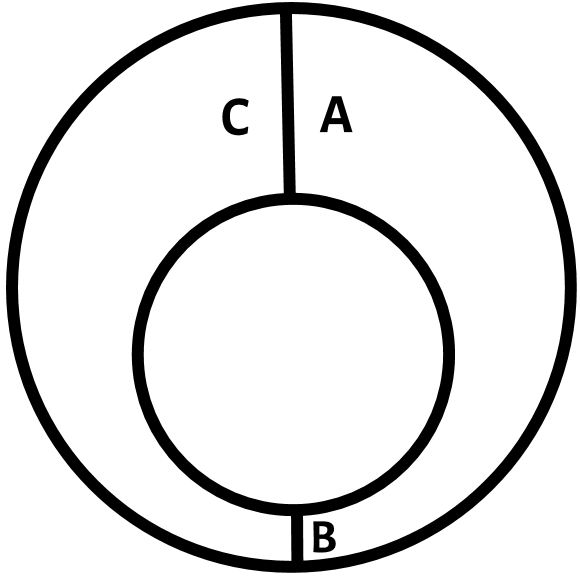
\includegraphics[width=1.25in,height=1.25in]{hegel-img002.png}
\end{center}
\item \label{bkm:Ref474665968}К стр. \pageref{bkm:bm48}. — Гегель дает здесь
в весьма вольном переводе и с перестановкой отдельных предложений
рассуждения Спинозы о бесконечном множестве неравных расстояний между двумя
неконцентричными окружностями (см. Спиноза, Переписка, М.~1932, стр.~78).
Конец приводимой Гегелем цитаты у Спинозы гласит: «...природа этой вещи не
может быть выражена никаким числом».
\item \label{bkm:Ref474666121}К стр. \pageref{bkm:bm49}. — В немецком тексте
вместо  стоит , а вместо  $(x+i)^n$ напечатано . Явная опечатка.
\item \label{bkm:Ref474666136}К стр. \pageref{bkm:bm50}. — Проверка с
помощью числа девять —~громоздкий искусственный прием, в настоящее время
вышедший из употребления, ввиду своей непрактичности.
\item \label{bkm:Ref474666147}К стр. \pageref{bkm:bm51}. — т.~е. «ведь эти
члены не будут иметь {\em никакого} значения» (или: «{\em никакого}
веса», «{\em никакой} силы»).
\item \label{bkm:Ref474666169}К стр. \pageref{bkm:bm52}. — См. стр.
\pageref{bkm:bm52a}–\pageref{bkm:bm52b}.
\item \label{bkm:Ref474666189}К стр. \pageref{bkm:bm53}. — Под
«Entwicklungspotenz» Гегель, как видно из этого места, а также из первого
абзаца следующего примечания («Еще другие формы, находящиеся в связи с
качественной определенностью величины», — стр. \pageref{bkm:bm53a}),
понимает то же самое, что в других местах он обозначает терминами:
«Entwicklungsglied» (член ряда, получающегося при разложении двучлена  по
формуле Ньютона), «Entwicklungsfunktion» (функция, получающаяся в
результате разложения в ряд, — «функция развертывания», как иногда
приходится переводить это выражение: см. напр. стр. \pageref{bkm:bm53b}),
«die Funktion der Potenzierung» (функция возвышения в степень),
«abgeleitete Funktion» (производная функция,— обычный в математике термин
для обозначения того, о чем здесь идет речь у Гегеля). Употребляя для
обозначения производной функции несколько странное выражение
«Entwicklungspotenz», Гегель, по-видимому, хочет подчеркнуть существенное
значение того обстоятельства, что дело идет тут именно о {\em степенных}
функциях, о разложении по {\em степеням}, о том, что интересующая нас
переменная величина {\em имеет степень выше первой} (см. выше, стр.
\pageref{bkm:bm53c}). Поэтому как первоначальную, так и производную функцию
Гегель называет «{\em степенными} функциями» (Potenzenfunktionen).
\end{enumerate}
В связи с этим нельзя не привести отзыв Энгельса. В письме Марксу от 18
августа 1881 г. Энгельс, говоря о математических рукописях Маркса, замечает
по поводу математических примечаний Гегеля: «Старик Гегель... вполне
правильно угадал, говоря, что дифференцирование в виде основного условия
требует, чтобы обе переменных имели различные степени и чтобы по меньшей
мере одна из них была во второй или $\frac 1 2$-й степени. Теперь мы уже знаем
почему». ({\em Маркс} и {\em Энгельс}, Соч., т.~XXIV, стр.~531–532).

\begin{enumerate}
\item \label{bkm:Ref474666244}К стр. \pageref{bkm:bm54}. — См. прим.
\ref{bkm:Ref474666189}.
\item \label{bkm:Ref474666256}К стр. \pageref{bkm:bm55}. — В немецком тексте
вместо «verglichen» стоит «vergleichen». По-видимому, это опечатка.
\item \label{bkm:Ref474666305}К стр. \pageref{bkm:bm56}. — Здесь слово «нуль»
употребляется Гегелем в фигуральном смысле —~в том смысле, что сторона
обратного отношения перестает быть стороной отношения, если она становится
равной показателю. В математическом же смысле, если мы возьмем обратное
отношение, показателем которого является произведение членов отношения  и
приравняем один из членов отношения этому произведению (например, ), то
другой член отношения будет не нулем, а единицей (у = 1). В арифметическом
обратном отношении (о котором здесь у Гегеля еще нет речи и формулой
которого является $х+у=С$), действительно, если $х=C$,
то $у=0$.
\item \label{bkm:Ref474666541}К стр. \pageref{bkm:bm57}. — В немецком тексте
вместо «keine» (никакой) стоит «eine». По-видимому, это опечатка.
\item \label{bkm:Ref474666560}К стр. \pageref{bkm:bm58}. — В издании Лассона
эта часть фразы дается по 1-му изданию «Науки логики», где эта фраза
гласит: «И вот определенное количество, которое отныне уже не есть
безразличное или внешнее определение, а дано так, что оно вместе с тем
снято как такое определение...» и~т.~д.
\item \label{bkm:Ref474666566}К стр. \pageref{bkm:bm59}. — Гегель имеет в
виду философию Шеллинга.
\item \label{bkm:Ref474666577}К стр. \pageref{bkm:bm60}. — Английское слово
«фут» означает прежде всего «нога, ступня», а затем уже «фут» в смысле меры
длины, приблизительно соответствующей длине ступни человека
(30,5~{\em см}). То же самое имеет место и в немецком языке со словом
«Fuss».
\item \label{bkm:Ref474666643}К стр. \pageref{bkm:bm61}. — Слово «правило»
(die Regel) Гегель употребляет здесь в смысле «мерило», «масштаб», «норма»,
«образцовая или указная мера» (Massregel, Richtmass). В XVIII в. слово
«Regel» иногда употреблялось в смысле линейки с делениями. Гегель,
по-видимому, и намекает на это старинное значение.
\item \label{bkm:Ref474666655}К стр. \pageref{bkm:bm62}. — Гегель
рассматривает здесь понятие физической {\em константы},~т.~е. того
эмпирического коэффициента, который в той или иной форме входит в уравнения
механики и физики. В качестве примера такой константы Гегель в следующей
фразе приводит величину $а$ в уравнении движения падения тел 
$s=at^2$. Гораздо чаще формулу движения падения тел
выражают уравнением $s=\frac 1 2 gt^2$, где константа
$g$ (постоянное для данного географического пункта ускорение силы
тяжести) равна приблизительно $9,8 \text{\em м}$ (в качестве единицы времени
берется при этом секунда). Следовательно, величина $а$ в уравнении
равна приблизительно $4,9 \text{\em м}$. Впрочем, надо сказать, что величина
$а$ или $g$, входящая в формулу движения падения тел, может
быть названа константою лишь в весьма относительном смысле. Дело в том, что
сама она изменяется с изменением расстояния от центра земного шара (а также
от расположения тяжелых масс на земной поверхности вблизи того места, где
производятся опыты с падением тел). Но так как эти изменения весьма
незначительны в тех случаях падения тел, которые рассматриваются в
элементарной механике (т.~е. в тех случаях, где расстояния, проходимые
падающим телом, незначительны по сравнению с длиной земного радиуса, причем
опыты производятся в одном и том же месте земной поверхности), то ими
вполне можно пренебречь.
\item \label{bkm:Ref474666676}К стр. \pageref{bkm:bm63}. — Здесь, как и в
предыдущем разделе «Мера как ряд отношений мер», Гегель имеет в виду учение
шведского химика Торберна Бергмана (1735–1784) о количественном выражении
сродства между основаниями и кислотами. Бергман предполагал, что одно и то
же количество какого-нибудь химического основания тем больше требует
кислоты для своего насыщения или нейтрализации, чем больше у них сродства
друг с другом. Он нашел, что для насыщения, например, 100 весовых частей
едкого кали требуется 78,5 весовых частей серной кислоты, или 64 весовых
частей азотной кислоты, или 51,5 весовых частей соляной кислоты и~т.~д.;
для насыщения же 100 весовых частей едкого натра нужно 177 весовых частей
верной кислоты, либо 135,5 весовых частей азотной кислоты, либо 125 весовых
частей соляной кислоты и~т.~д. В том и другом случае {\em порядок}
кислот остается {\em один и тот же}. Получается некоторой ряд пропорций
или мер насыщения (нейтрализации), который, по Гегелю, и характеризует
собой специфическую природу исследуемого вещества, выступающего в качестве
{\em противочлена} этого ряда. Учение Бергмана о химическом сродстве и
его количественном выражении было господствующей теорией в последней
четверти XVIII в. В начале XIX в. появилась новая теория химического
сродства, связанная с именем французского химика Клода Бертоллэ
(1748–1822), в значительной мере направленная против теории Бергмана.
Бертоллэ считал, что, наоборот, чем меньшее количество вещества $А$
требуется для нейтрализации вещества $В$, тем больше сродство между
ними. Кроме того, также и числовые значения мер насыщения, найденные
Бергманом, оказались при более тщательных экспериментах весьма неточными.
Сочинения Бергмана были изданы в немецком переводе в 1782–1799 гг. и были
широко известны в Германии. Между прочим, от Бергмана идет термин
«attractio electiva» (избирательное притяжение), который в немецком
переводе был передан термином «Wahlverwandtschaft» (избирательное
сродство), употребляемым здесь у Гегеля для обозначения одной из категорий
меры. Подробнее о теориях Бергмана и Бертоллэ см. у {\em Hermann Корр},
Geschichte der Chemie, Neudruck der Originalausgabe, Leipzig 1931, Bd. II,
S. 297–324, откуда и взяты вышеприведенные сведения. — Что касается
«избирательного сродства», как химической категории, то принцип этого
сродства был сформулирован еще задолго до Бергмана французским химиком
Этьеном Жоффруа (1672–1731), который в 1718 г. выставил следующее
положение: «Всякий раз, когда мы имеем соединение двух веществ, обладающих
склонностью соединяться друг с другом, если к этому соединению
примешивается третье вещество, имеющее более сильное сродство с одним из
первых двух, то это третье вещество соединяется с ним, отбивая его от
другого» (цитировано у Коппа, стр.~296 второго тома),~т.~е. указанное
третье вещество разлагает первоначально данное соединение, соединяясь с
одним из компонентов и вытесняя из соединения другой компонент.
\item \label{bkm:Ref474666698}К стр. \pageref{bkm:bm64}. — Имеется в виду
учение Бергмана (см. предыдущее примечание).
\item \label{bkm:Ref474666706}К стр. \pageref{bkm:bm65}. — «Учебник химии»
Берцелиуса вышел в трех томах в 1808–1828 гг.
\item \label{bkm:Ref474666715}К стр. \pageref{bkm:bm66}. — Гегель неправ:
причиной остановки маятника является не сила тяжести, а трение в том месте,
где маятник прикреплен или привязан, а также и сопротивление воздуха (или
какой-нибудь другой среды, в которой качается маятник).
\item \label{bkm:Ref474666719}К стр. \pageref{bkm:bm67}. — Немецкий текст
здесь испорчен. Перевод сделан на основе конъектуры Б. Г. Столпнера,
предлагающего вместо «eintretender qualitativer Bestimmtheit» читать
«eintretende qualitative Bestimmtheit». Лассон предлагает другую
конъектуру, вставляя перед указанными словами слова «ein Unterschied». В
этом случае надо было бы перевести эту фразу следующим образом: «Если,
таким образом, различие химического сродства, в противоположность
избирательному сродству, точно устанавливается в некотором ряде
количественных отношений, как различие появляющейся качественной
определенности...» и~т.~д.
\item \label{bkm:Ref474666725}К стр. \pageref{bkm:bm68}. — Имеются в виду
электрохимические теории английского химика Дэви (1778—1829) и шведского
химика Берцелиуса (1779–1848), явившиеся крупным шагом вперед в развитии
химии. Гегель недооценивал их значение, так же, как он недооценивал
прогрессивное значение химических теорий Бертоллэ.
\item \label{bkm:Ref474666740}К стр. \pageref{bkm:bm69}. — Выражение
«индифференция» (неразличенность, безразличие) было употреблено Шеллингом в
его вышедшей в 1801 г. работе «Изложение моей системы философии» для
обозначения «абсолютного тождества» субъекта и объекта. «Совершенная
неразличенность (totale Indifferenz) субъективного и объективного» —~таково
было основное понятие этой фазы философского развития Шеллинга. В
дальнейшем Гегель подробно рассматривает шеллинговскую концепцию
«индифференции как обратного отношения между ее факторами» и подвергает ее
имманентной критике, вскрывая ее «всестороннюю противоречивость». По учению
Шеллинга абсолютное представляет собою неподвижное тождество, полнейшую
неразличенность, совершенное безразличие двух факторов: субъективного и
объективного. Всякое же дифференцирование состоит лишь в количественном
перевесе одного из этих двух факторов над другим, причем «вечным основанием
и опорою всех количественных различий субъективного и объективного служит
их совершенная индифференция, составляющая форму абсолютного тождества,
форму их бесконечного бытия» (см. {\em Куно Фишер}, Шеллинг, его жизнь,
сочинения и учение, пер. H. Лocского, Спб. 1905, стр. 590). О шеллинговой
системе «абсолютного тождества» Гегель упоминал также и выше, на
стр.~\pageref{bkm:bm69a}. Ср. прим.~\ref{bkm:Ref474665876} к этому месту.
\item \label{bkm:Ref474666761}К стр. \pageref{bkm:bm70}. — См. предыдущее
примечание.
\item \label{bkm:Ref474666774}К стр. \pageref{bkm:bm71}. — В первом издании
«Науки логики» (1812) здесь стояла еще следующая фраза, выпущенная Гегелем
в 1831 г., когда он готовил второе издание: «Этот вопрос я осветил в моей
более ранней диссертации, где я доказал несостоятельность этого различения
и построенных на нем объяснений». Имеется в виду «Философская диссертация
об орбитах планет» (1801) Возможно, что Гегель выпустил эту ссылку на свою
диссертацию потому, что в ней, между прочим, доказывалось, что между
Юпитером и Марсом не может быть никаких планет, между тем как еще в 1801 г.
была открыта малая планета Церера, расположенная как раз между Юпитером и
Марсом.
\item \label{bkm:Ref474666782}К стр. \pageref{bkm:bm72}. — Это не совсем
так. Как уже было упомянуто в примечании \ref{bkm:Ref474665489}{}-м, Гегель
в значительной мере произвольно толковал философию Спинозы, приписывая ей
акосмизм (отрицание мира) и идеализм. В этом отношении он шел по стопам
Шеллинга, использовавшего некоторые элементы спинозизма для построения
своей идеалистической философии «абсолютного тождества». В действительности
же между материалистом Спинозой и объективным идеалистом Шеллингом огромная
принципиальная разница, и эта-то разница как раз и смазывается в
гегелевской трактовке спинозизма.
\item \label{bkm:Ref474666794}К стр. \pageref{bkm:bm73}. — См. «Учение о
бытии», стр. \pageref{bkm:bm73a}—\pageref{bkm:bm73b}.
\item \label{bkm:Ref474666798}К стр. \pageref{bkm:bm74}. — В немецком тексте
вместо sie (т.~е. Negation) стоит es. По-видимому, это опечатка.
\item \label{bkm:Ref474666813}К стр. \pageref{bkm:bm75}. — См. примечание
\ref{bkm:Ref474665836}.
\item \label{bkm:Ref474666829}К стр. \pageref{bkm:bm76}. — См.
{\em Кант}, Критика способности суждения, пер. Н. Соколова, Спб. 1898,
стр. 16—17.
\item \label{bkm:Ref474666833}К стр. \pageref{bkm:bm77}. — Здесь кончается
выписка из «Критики способности суждения» (стр. XXVI немецкого издания 1799
г., стр.~16 русского перевода).
\item \label{bkm:Ref474666843}К стр. \pageref{bkm:bm78}. — Гегель имеет в
виду Шеллинга и его последователей. Шеллинг начиная с 1800 г., когда он
выпустил свою «Систему трансцендентального идеализма», выдвигает в качестве
«органа всякого трансцендентального мышления» «интеллектуальную интуицию»,
как непосредственное созерцание абсолютного, целиком противоположное
рассудочному познанию и совершенно оторванное от него. Против шеллинговой
«интеллектуальной интуиции» Гегель впервые выступил в начале 1807 г в
предисловии к «Феноменологии духа». В своих «Лекциях по истории философии»
Гегель дает более развернутую критику Шеллинга и его поклонников. Особенно
резко он отзывается об этих последних. «Вся эта тенденция, — говорит он об
антинаучном характере философских упражнений шеллингианцев, —
противопоставляет себя прежде всего {\em рефлективному мышлению}, или,
иначе сказать, такому движению рассуждения, которое держится фиксированных,
прочных, неподвижных понятий. Но вместо того чтобы оставаться в области
понятия и познать его как беспокойное «я», они впали в противоположную
крайность покоящегося созерцания, непосредственного бытия, неподвижного «в
себе» и полагают, что этот недостаток, эта неподвижность, исправляется
глядением и что это глядение они превращают в интеллектуальное, определяя
его в свою очередь посредством какого-нибудь фиксированного понятия»
({\em Гегель}, Лекции по истории философии, кн.~III. М.—Л. 1936,
стр.~511).
\end{enumerate}
Самое слово «рефлексия» Гегель употребляет в различных значениях, притом
так, что одно значение незаметно переходит у него в другое или даже
совмещается с другим. Латинское слово «reflexio» означает «загибание назад,
отклонение назад, отражение» (света, звуковой волны, брошенного во
что-нибудь предмета). В новых языках это слово наряду с этим значением
«отражения» приобрело еще значение «размышления, обдумывания, рассуждения,
соображения, рассудительности» (мысль как бы оборачивается на самоё себя,
отражается в себя самоё). У Гегеля рефлексия берется то в объективном, то в
субъективном смысле. При этом Гегель, как объективный и абсолютный
{\em идеалист}, понимает объективную рефлексию не в смысле взаимного
отражения сторон или моментов материального предмета друг другом или друг в
друге и не в смысле обратного их отражения в себя самих, а в смысле
взаимного отражения между определениями понятия как такового или в смысле
обратного отражения какого-нибудь понятийного определения внутрь себя
самого («рефлексия в себя»). Субъективную же рефлексию Гегель, как
идеалист, берет не в смысле гносеологического отражения объективно-реальной
материальной действительности в человеческом или животном сознании, а в
смысле рассудочного оперирования абстрактными категориями чистой мысли.
Рефлексия рассудка подвергается у Гегеля уничтожающей критике в том случае,
если она выступает с претензией на полное, завершенное, абсолютное
познание. Но вместе с тем Гегель решительно защищает эту рефлексию рассудка
как необходимый момент в диалектическом развитии познания (против Шеллинга
и шеллингианцев, против Якоби и против романтиков). Рефлексия в себя и
рефлексия в другое (притом не в другое вообще, а в «{\em свое} другое»)
составляют, по Гегелю, характерную черту категорий сущности (которая ведь
представляет собою «абсолютное опосредствование с собою»), точно так же как
переход от одного к другому был характерной чертой категорий бытия (где
господствует непосредственность), а развитие или развертывание
(Entwickelung) будет характерной чертой категорий понятия (где имеет место
единство непосредственного и опосредствованного).

В теснейшей связи с выражением «рефлексия» Гегель употребляет выражение
«Scheinen», имеющее у него опять-таки специфически-метафорическое значение.
«Das Scheinen» означает у Гегеля «свечение, мерцание, отблеск» (например,
Гегель говорит, что положительное «светится» в отрицательном, а
отрицательное —~в положительном; см. в тексте стр. \pageref{bkm:bm78a}).
Иногда Гегель приводит выражение «Scheinen» в прямою связь с термином
«Schein» (видимость, кажимость), и тогда «das Scheinen» приходится
переводить словами «свечение видимостью» (в себе самом или в своем другом),
или «излучение видимости» (в себя самого или в свое другое).

\begin{enumerate}
\item \label{bkm:Ref474666865}К стр. \pageref{bkm:bm79}. — В немецком тексте
(как в издании Глокнера, так и в издании Лассона) вместо слова
«положительным» стоит слово «отрицательным». По-видимому, это опечатка.
\item \label{bkm:Ref474666880}К стр. \pageref{bkm:bm80}. — В немецком тексте
наоборот: «+~а раз –~а». По-видимому, это опечатка.
\item \label{bkm:Ref474666891}К стр. \pageref{bkm:bm81}. — Об игре слов в
немецком выражении «zu Grunde gehen», как его употребляет Гегель, см.
замечания Энгельса в письмах Конраду Шмидту от 1 ноября 1891 г. и от 4
февраля 1892 г. ({\em Маркс} и {\em Энгельс}, Письма, под ред.
Адоратского, изд. 4-е, М.—Л. 1931, стр. 393–394).
\item \label{bkm:Ref474666904}К стр. \pageref{bkm:bm82}. — Слово «этиология»
(от греческого «aitia» —~причина, начало, основание) означает учение о
причинах, указание причин или оснований для тех или иных явлений.
\item \label{bkm:Ref474666911}К стр. \pageref{bkm:bm83}. — Лассон считает,
что придаточное предложение «что растение имеет свое основание в
производящей растения силе» попало сюда по ошибке и должно быть поставлено
двумя строчками выше, после слов «я скажу, что оно есть растение».
Стилистически такая перестановка улучшает конструкцию всей этой фразы, но
логический смысл заставляет предпочесть тот текст, какой дается в издании
Глокнера. С этого текста и сделан перевод этой фразы с добавлением слов
«того предложения» перед приведенным выше придаточным предложением.
\item \label{bkm:Ref474666923}К стр. \pageref{bkm:bm84}. — т.~е. по-своему,
по-разному.
\item \label{bkm:Ref474666940}К стр. \pageref{bkm:bm85}. — См. «Учение о
бытии», стр. \pageref{bkm:bm85a}–\pageref{bkm:bm85b}.
\item \label{bkm:Ref474667017}К стр. \pageref{bkm:bm86}. — В русском
переводе под ред. Радлова ({\em Гегель}, Феноменология духа, Спб. 1913)
это место находится на стр. 72—74 (в главе «Сила и рассудок, явление и
сверхчувственный мир»).
\item \label{bkm:Ref474667030}К стр. \pageref{bkm:bm87}. — В немецком
тексте: «das Relative eines Ändern». По-видимому, это опечатка вместо: «das
Relative seines Ändern».
\item \label{bkm:Ref474667041}К стр. \pageref{bkm:bm88}. — См. часть первая,
стр. \pageref{bkm:bm88a}–\pageref{bkm:bm88b}.
\item \label{bkm:Ref474667057}К стр. \pageref{bkm:bm89}. — В немецком
тексте: «in derselben». По-видимому, это опечатка вместо: «in demselben».
\item \label{bkm:Ref474667072}К стр. \pageref{bkm:bm90}. — Ср. замечание
Энгельса о том, что «сила имеет точно такую же величину, как и ее
проявление во-вне, ибо в них обоих совершается {\em одно и то же
движение}» ({\em Engels}, Herrn E. Dührings Umwälzung der Wissenschaft.
Moskau —~Leningrad 1935, S.~64).
\item \label{bkm:Ref474669620}К стр. \pageref{bkm:bm91}. — См. примечания
\ref{bkm:Ref474665489} и \ref{bkm:Ref474666782}.
\item \label{bkm:Ref474669634}К стр. \pageref{bkm:bm92}. — Это не точно. 4-я
дефиниция первой части «Этики» гласит: «Под атрибутом я разумею то, что
интеллект мыслит о субстанции, как составляющее ее сущность». Из
сопоставления этой дефиниции с рядом других мест из «Этики» и из
«Переписки» Спинозы видно, что атрибуты, но учению Спинозы, не только
{\em мыслятся} интеллектом как составляющие сущность субстанции, но и
действительно «выражают, раскрывают и составляют вечную сущность и вечное
существование» субстанции безотносительно к интеллекту (см., например,
доказательства теоремы 19-й и 20-й первой части «Этики» и письмо 2-е).
Субстанция, говорит Спиноза, {\em имеет} атрибуты (доказательство
теоремы 16-й первой части «Этики»).
\item \label{bkm:Ref474669669}К стр. \pageref{bkm:bm93}. — Абсолютная
необходимость слепа потому, что она равносильна абсолютной случайности, как
это более определенно намечается Гегелем в непосредственно следующих за
этим рассуждениях, содержащих элементы диалектической критики категории
абсолютной необходимости. Если все одинаково абсолютно-необходимо, если
все, что существует, существует только потому, что оно существует, не имея
для своего существования никаких других оснований, то это значит, что все
абсолютно случайно. Здесь получается {\em непосредственное} или, как
выражается Гегель, намекая, по-видимому, на Шеллинга (а также, без сомнения,
и на метафизический детерминизм Спинозы), «{\em абсолютное}» тождество
сущности и бытия, возможности и действительности, необходимости и
случайности —~такое тождество, где отсутствует самодвижение, где имеется
лишь «рефлексия в себя» без «рефлексии в другое». Сама сущность выступает
здесь в форме «бытия», в форме простой непосредственности, простого факта.
Подобно тому, как ночью, согласно немецкой поговорке, «все коровы черны»
(или, согласно русской поговорке, «все кошки серы»), так и в «одноцветном»
абсолюте Шеллинга все совершенно одинаково {\em по своей форме}, все
различия между отдельными категориями стерты, растворены в «пустой бездне»
({\em Гегель}, Феноменология духа, предисловие, стр. 12 в немецком
издании Лассона, Лейпциг 1921, или стр. 7 в русском переводе под ред.
Радлова, Спб. 1913). Что касается специально абсолютной необходимости, то
возможность абсолютно-необходимого и его действительность непосредственно
совпадают именно потому, что все вещи и все события рассматриваются на
данном этапе как {\em одинаково} необходимые, как необходимости
{\em одного и того же порядка}. Ср. классические формулировки Спинозы:
«Из необходимости божественной природы должно следовать бесконечно многое
бесконечно-многими способами,~т.~е. все то, что может стать объектом
бесконечного интеллекта» («Этика», ч.~I, теор.~16); «из бесконечной природы
бога все всегда следует по одной и той же необходимости, точно таким же
образом, как из природы треугольника от века и до века следует, что его три
угла равны двум прямым» (там же, схолия к теор. 17). По Спинозе, все
отдельные вещи одинаково необходимы, но вместе с тем все они одинаково
случайны (см. королларий к теор. 31 второй части и дефиницию 3-ю четвертой
части).
\end{enumerate}
В своем гениальном отрывке о «Случайности и необходимости» Энгельс, отмечая
заслуги Гегеля по части диалектической трактовки категорий необходимости и
случайности, дает замечательный по своей глубине и ясности диалектический
анализ и диалектическую критику точки зрения абсолютной необходимости,
которую он характеризует как «механический детерминизм, который на словах
отрицает случайность в общем, чтобы на практике признать ее в каждом
отдельном случае» («Диалектика природы», изд. 1936 г., стр. 109).
Механический детерминизм, указывает Энгельс, «деградирует необходимость до
уровня случайности» (там же, стр. 108).

Известное положение Гегеля о том, что «слепа необходимость лишь постольку,
поскольку она не постигается в понятии» ({\em Гегель}, Собр. соч., т. I,
стр. 248; ср. {\em Энгельс}, Анти-Дюринг, гл. XI первого раздела),
нисколько не противоречит его трактовке абсолютной необходимости в
рассматриваемом месте, ибо абсолютная необходимость, провозглашаемая
механическим детерминизмом, по самому существу своему не может быть
объектом конкретного, адэкватного познания, не может быть «постигнута в
понятии». Поэтому Гегель и говорит, что в стадии абсолютной необходимости
(или, что то же самое, в стадии абсолютной действительности, абсолютного
факта) необходимость «заперта» в бытии, что она «боится света». В
дальнейшем, а именно при переходе от «Сущности» к «Понятию», необходимость
«раскроется» (ср. в тексте стр. \pageref{bkm:bm93a}) и тем самым перестанет
быть «слепой».

\begin{enumerate}
\item \label{bkm:Ref474669698}К стр. \pageref{bkm:bm94}. — Это предисловие
предпослано IV т. Собрания сочинений Гегеля, изданного вскоре после его
смерти его учениками, — тому, содержащему 2-ю часть «Науки логики»
—~«Учение о сущности».
\item \label{bkm:Ref474655210}К стр. \pageref{bkm:bm95}. — Имеется в виду
изречение Лессинга о том, что если бы бог предложил ему выбор между
готовой, законченной, чистой истиной и вечно живым стремлением к ней,
стремлением, связанным с постоянными ошибками и заблуждениями, то он выбрал
бы последнее. См. Lessings Philosophie, hrsg. von Paul Lorenz, Leipzig
1909, S. 106.
\end{enumerate}

\bigskip


\bigskip



\clearpage
\tableofcontents*
\clearpage

\end{document}
